\documentclass{book}
\usepackage[utf8]{inputenc}
\usepackage[T1]{fontenc}
\usepackage{lmodern}        % Fuentes vectoriales Type 1
\usepackage{microtype}      % Mejora la legibilidad
\usepackage[spanish]{babel}
\usepackage[margin=2.5cm]{geometry}
\usepackage{amsmath}
\usepackage{amssymb}
\usepackage{graphicx}
\usepackage{booktabs}
\usepackage{tabularx}
\usepackage{sidecap}
\usepackage{placeins}

\graphicspath{{imagenes/}}
\usepackage{url}

\AtBeginDocument{\shorthandoff{"}}

\begin{document}
\setcounter{chapter}{7}

% --- INICIO DEL CAPÍTULO 8 ---
\chapter{Sistema Cardiovascular}

\begin{flushleft}
    \textit{Se describen los componentes y el funcionamiento del sistema circulatorio humano, seguidos de una discusión detallada sobre las propiedades, la presión y el flujo de la sangre en él. Esto conduce al análisis de los aspectos físicos de los accidentes cerebrovasculares y los aneurismas. Se desarrollan y aplican modelos del sistema circulatorio y sus componentes al corazón normal y con disfunciones.}
\end{flushleft}

\hrule
\vspace{1em}

Existen tres componentes en el sistema cardiovascular. (a) La sangre es el vehículo para el transporte. Transporta el combustible del alimento digerido hacia las células, transporta el oxígeno del aire en los pulmones para que pueda combinarse con el combustible para liberar energía, y elimina los productos de desecho —tales como el dióxido de carbono del motor de combustible y otros desechos metabólicos—. (b) El sistema circulatorio es el sistema de distribución y consiste en una serie de vasos sanguíneos ramificados. (c) El corazón es la bomba de cuatro cavidades compuesta principalmente por músculo cardíaco que hace posible este flujo circulatorio. Se pueden encontrar descripciones generales del sistema cardiovascular en [5, 7, 10, 11, 14, 16, 23, 24, 27, 29, 36, 37, 40, 46, 57, 58, 66].

\section{Generalidades del sistema circulatorio y del ciclo cardíaco}

\subsection{Circulación}

El flujo sanguíneo proveniente del corazón se ramifica en dos sistemas separados (Fig.~8.1). En el sistema de circulación pulmonar, el lado derecho del corazón bombea sangre pobre en oxígeno («azul») hacia los pulmones para ser oxigenada; la sangre rica en oxígeno («roja») regresa luego al lado izquierdo del corazón. En el sistema de circulación sistémica, el lado izquierdo del corazón bombea esta sangre rica en oxígeno («roja») al resto del cuerpo donde es utilizada; la sangre pobre en oxígeno («azul») regresa luego al lado derecho del corazón. Esto ocurre en un sistema de arterias que conduce la sangre desde el corazón hacia los pulmones y otros órganos y componentes, y un sistema de venas que retorna la sangre al corazón.

\begin{figure}[htbp]
  \centering
  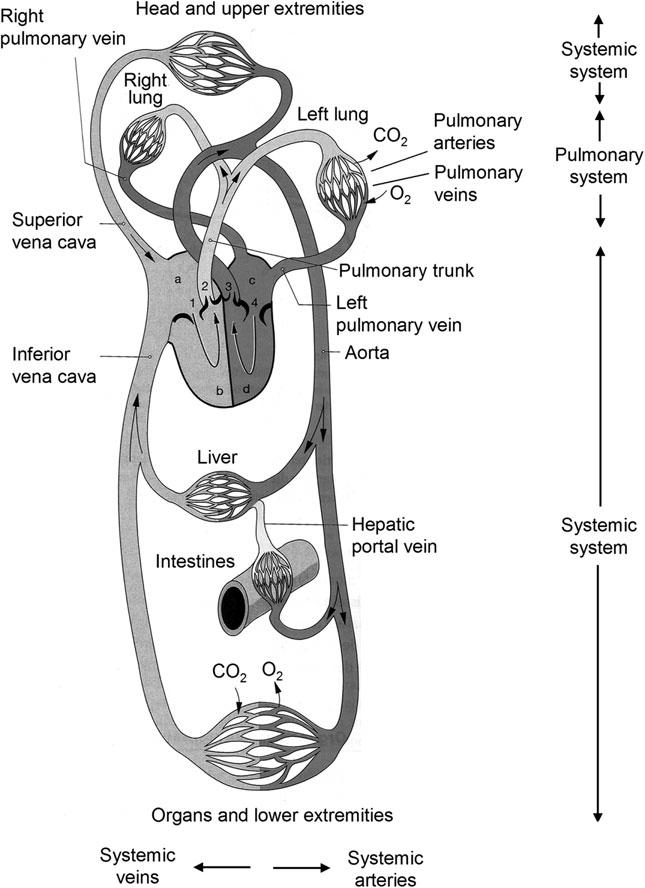
\includegraphics[width=0.45\textwidth]{81.png}
  \caption{Sistema de circulación sanguínea, y etiquetas dentro del corazón: a aurícula derecha, b ventrículo derecho, c aurícula izquierda, d ventrículo izquierdo, 1 válvula auriculoventricular derecha (tricúspide), 2 válvula semilunar pulmonar, 3 válvula semilunar aórtica, 4 válvula auriculoventricular izquierda (bicúspide, mitral) (De [65]).}
  \label{fig:81}
\end{figure}



En el sistema pulmonar (Fig.~8.1), la sangre ingresa a la aurícula derecha (AD) del corazón (Fig.~8.2) a través de las venas cavas inferior y superior. La sangre pasa a través de la válvula auriculoventricular derecha (o tricúspide) para ingresar al ventrículo derecho (VD). La sangre es bombeada primero a través de la válvula semilunar pulmonar hacia las arterias pulmonares, las cuales se ramifican en una serie de arterias menores y arteriolas, y luego hacia los capilares en los pulmones. Estos capilares pulmonares se combinan en vénulas, luego en venas más grandes y finalmente en las venas pulmonares.

\begin{figure}[htbp]
  \centering
  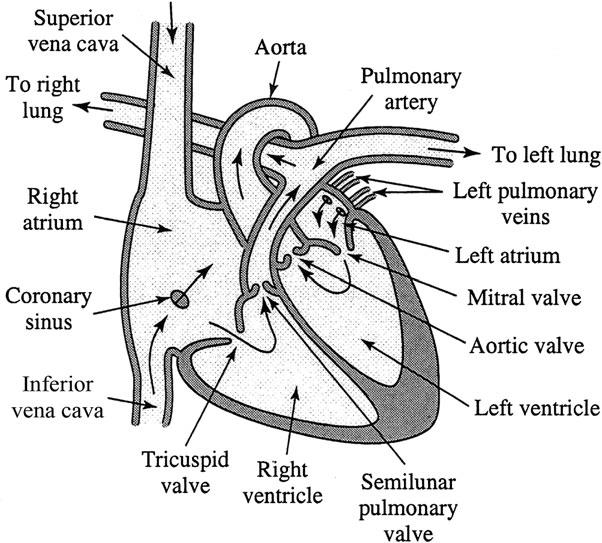
\includegraphics[width=0.7\textwidth]{82.png}
  \caption{Diagrama del corazón, con sus principales cavidades, válvulas y vasos (De [4]).}
  \label{fig:82}
\end{figure}



En el sistema sistémico (Fig.~8.1), la sangre ingresa a la aurícula izquierda (AI) del corazón a través de las venas pulmonares. La sangre pasa a través de la válvula auriculoventricular izquierda (o bicúspide o mitral) para ingresar al ventrículo izquierdo (VI). La sangre es bombeada a través de la válvula semilunar aórtica hacia la aorta, la cual se ramifica primero en una serie de arterias principales y luego en arterias menores (las arteriolas, con diámetros más pequeños), y finalmente en una serie de capilares en los sistemas donde ocurren el intercambio gaseoso y la difusión. Estos capilares sistémicos se combinan en vénulas, luego en venas más grandes y finalmente en las venas cavas superior (desde arriba del corazón) e inferior (desde abajo del corazón).

(Una regla mnemotécnica útil para el flujo de sangre en el corazón proviene de saber que el autor vivió una vez en Rahlves Drive en Castro Valley, California —una ciudad aproximadamente $20\text{ millas}$ al sur de Berkeley—. Todo el ciclo cardíaco comienza con la sangre fluyendo hacia la aurícula derecha (AD) y luego oxigenándose en los pulmones, regresando al corazón (C), y luego continuando con la sangre que sale del ventrículo izquierdo (VI) y sale (S) hacia los sistemas (S). En inglés, esto se deletrea RAHLVES [RA (AD) + H (C) + LV (VI) + E (salida) + S (sistemas)]. El concepto más importante aquí es que la sangre desoxigenada ingresa al corazón a través de la aurícula derecha (AD) y eventualmente la sangre oxigenada sale a través del ventrículo izquierdo (VI) del corazón para ser utilizada por el cuerpo para el metabolismo. Para algunos, puede ser más fácil recordar que el estadounidense Daron Rahlves fue el ganador de la competencia de esquí de descenso super-G en el Campeonato Mundial de 2001).

\begin{table}[htbp]
\centering
\caption{Valores normales en reposo de la presión sanguínea, con los volúmenes del sistema}
\label{tab:81}
\small
\begin{tabularx}{0.8\textwidth}{X >{\centering\arraybackslash}p{3cm} >{\centering\arraybackslash}p{3cm}}
\toprule
\textbf{Sistema} & \textbf{$P\ (\text{mmHg})$} & \textbf{$V\ (\text{L})$} \\
\midrule
Arterias sistémicas & $100$ & $1{,}0$ \\
Venas sistémicas & $2$ & $3{,}5$ \\
Arterias pulmonares & $15$ & $0{,}1$ \\
Venas pulmonares & $5$ & $0{,}4$ \\
\bottomrule
\end{tabularx}
\end{table}

Los sistemas sistémico y pulmonar tienen similitudes y diferencias. Tienen el mismo caudal volumétrico $Q$ promediado sobre un latido cardíaco. (Si no fueran iguales, la sangre tendría que acumularse o fugarse en alguna parte). Este es de ${\sim}5\text{--}6\text{ L/min}$, y también es igual al caudal promedio de sangre bombeada por el corazón, el gasto cardíaco. En el sistema sistémico la sangre se desprende de oxígeno y recibe dióxido de carbono, mientras que en el sistema pulmonar la sangre se desprende de dióxido de carbono y recibe oxígeno. La Tabla~8.1 muestra que el sistema sistémico tiene presiones más altas (en las arterias) y volúmenes mayores que el sistema pulmonar (incluso con el mismo $Q$). Esta diferencia de presión tiene sentido porque los vasos sanguíneos necesitan ser más largos para llegar a regiones más distantes en el cuerpo en el sistema sistémico. El corazón izquierdo ($\text{AI} + \text{VI}$) es más grande (y es una bomba mayor) que el corazón derecho ($\text{AD} + \text{VD}$) debido a esta necesidad de generar una presión más alta para la circulación sistémica. Las paredes del corazón consisten principalmente en la capa muscular media gruesa, el miocardio, el cual está revestido internamente por una fina capa de tejido, el endocardio, y externamente por una membrana, el epicardium (epicardio). Los dos lados del corazón están separados por un tabique (septum). La diferencia de volumen se debe a la mayor distancia de recorrido y al número mucho mayor de sistemas que reciben sangre en el sistema sistémico. La Tabla~8.1 también muestra que las arterias tienen una presión más alta que las venas correspondientes, mientras que las venas tienen volúmenes mayores. El volumen total de sangre es de $\simeq 5\text{ L}$.

Para una persona en reposo, el $12\%$ de la sangre se encuentra en las cavidades del corazón, el $2\%$ en la aorta, el $8\%$ en las arterias, el $1\%$ en las arteriolas, el $5\%$ en los capilares, el $50\%$ en las venas sistémicas y el $18\%$ en la circulación pulmonar.

Las arterias y venas principales se muestran en las Figs.~8.3 y 8.4. Las Tablas~8.2 y 8.3 proporcionan una cuantificación muy aproximada de los vasos en el sistema circulatorio. La Tabla~8.4 proporciona información más específica sobre algunas de las arterias principales o grandes [57]. Existe un estrechamiento (conicidad) a lo largo de la longitud de la mayoría de las arterias grandes (Tabla~8.4), donde la disminución del radio arterial se puede modelar como un decaimiento exponencial lento [57]. Las arterias pequeñas se pueden modelar asumiendo que no tienen estrechamiento. La longitud $L$ de una arteria más pequeña se puede estimar a partir de su diámetro $d$ mediante $L/d \sim 25$.

\begin{figure}[htbp]
  \centering
  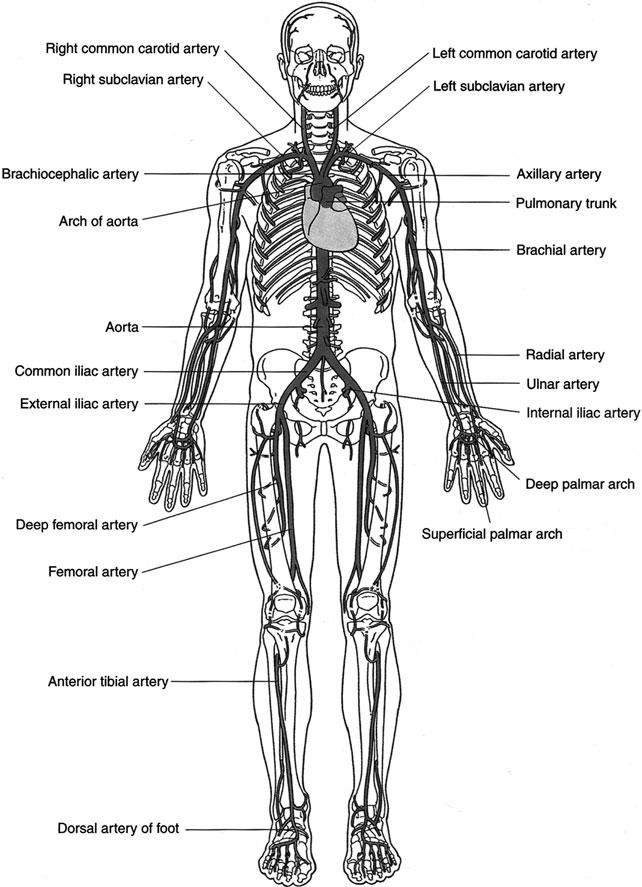
\includegraphics[width=0.45\textwidth]{83.png}
  \caption{Arterias principales en el cuerpo. Las arterias transportan sangre desde el corazón en los sistemas sistémico y pulmonar. Muchas vienen en pares, como las arterias radiales derecha e izquierda (De [53]. Usado con permiso).}
  \label{fig:83}
\end{figure}

\begin{figure}[htbp]
  \centering
  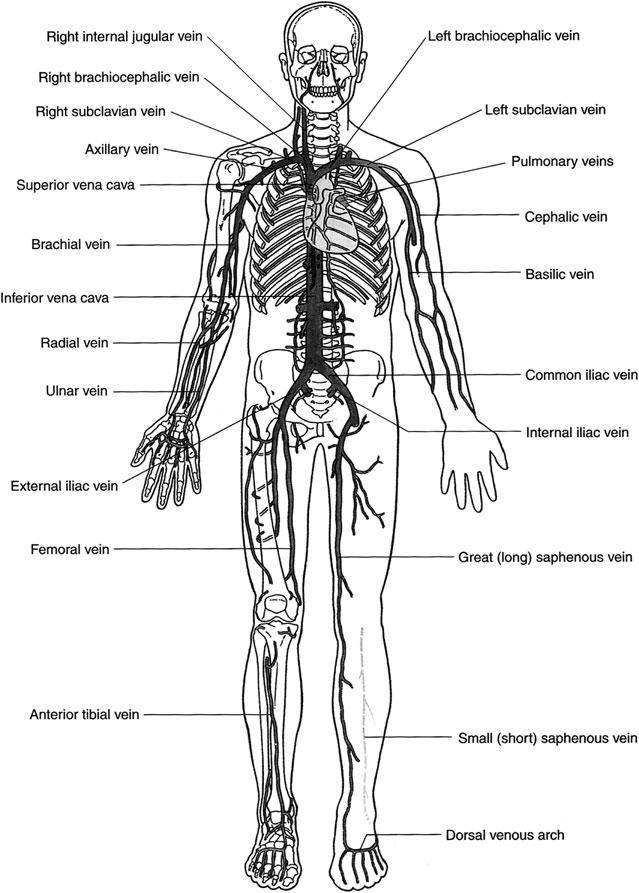
\includegraphics[width=0.45\textwidth]{84.png}
  \caption{Venas principales en el cuerpo. Solo se muestran las venas superficiales en las extremidades izquierdas y solo las venas profundas en las extremidades derechas. Las venas transportan la sangre de regreso al corazón en los sistemas sistémico y pulmonar. Muchas vienen en pares, como las venas radiales derecha e izquierda (De [53]. Usado con permiso).}
  \label{fig:84}
\end{figure}



En el árbol arterial, las arterias se bifurcan en dos más pequeñas, siendo el área de la sección transversal de cada vaso hijo menor que la del vaso padre, pero su suma es mayor [57]. La bifurcación normalmente no es simétrica, siendo el vaso hijo más grande una continuación del vaso padre. En las ${\sim}26$ generaciones de bifurcaciones, el área de la sección transversal total de las arterias aumenta aproximadamente cien veces desde la aorta hasta las arteriolas pequeñas ($0{,}003\text{ cm}$ de diámetro), ocurriendo el primer aumento de cinco veces desde la aorta hasta las arterias grandes. Para las arterias pequeñas, los radios de la arteria padre $r_{\text{p}}$ y de los vasos hijos $r_{\text{d1}}$ y $r_{\text{d2}}$ se han relacionado mediante tres relaciones (las cuales no son independientes entre sí): $r_{\text{p}}^\xi = r_{\text{d1}}^\xi + r_{\text{d2}}^\xi$ con $\xi = 2{,}76$, $\gamma = (r_{\text{d2}}/r_{\text{d1}})^2 = 0{,}41$ y $\eta = (r_{\text{d1}}^2 + r_{\text{d2}}^2)/r_{\text{p}}^2 = 1{,}16$ [57]. (Véanse también los Problemas 8.34 al 8.37).

\begin{table}[htbp]
\centering
\caption{Cuantificación aproximada de vasos individuales en el sistema circulatorio humano}
\label{tab:82}
\small
\begin{tabularx}{\textwidth}{X *{4}{>{\centering\arraybackslash}p{2.3cm}}}
\toprule
\textbf{Vaso} & \textbf{Diámetro ($\text{mm}$)} & \textbf{Longitud ($\text{mm}$)} & \textbf{Espesor de pared ($\mu\text{m}$)} & \textbf{Presión ($\text{mmHg}$)} \\
\midrule
Aorta & $25{,}0$ & $400$ & $1\,500$ & $100$ \\
Arterias grandes & $6{,}5$ & $200$ & $1\,000$ & $100$ \\
Ramificaciones arteriales principales & $2{,}4$ & $100$ & $800$ & $95$ \\
Ramificaciones arteriales terminales & $1{,}2$ & $10$ & $125$ & $90$ \\
Arteriolas & $0{,}1$ & $2$ & $20$ & $60$ \\
Capilares & $0{,}008$ & $1$ & $1$ & $30$ \\
Vénulas & $0{,}15$ & $2$ & $2$ & $20$ \\
Vénulas terminales & $1{,}5$ & $10$ & $40$ & $15$ \\
Ramificaciones venosas principales & $5{,}0$ & $100$ & $500$ & $15$ \\
Venas grandes & $14{,}0$ & $200$ & $800$ & $10$ \\
Vena cava$^{\text{a}}$ & $30{,}0$ & $400$ & $1\,200$ & $5$ \\
Cavidades del corazón & -- & -- & -- & $120$ \\
\bottomrule
\end{tabularx}
\begin{flushleft}
    \small Usando datos de [21].\\
    Este estudio es para un varón de $30\text{ años}$ de edad, con una masa de $70\text{ kg}$ y un volumen de sangre de $5{,}4\text{ L}$.\\
    $^{\text{a}}$ En realidad existen dos venas cavas.
\end{flushleft}
\end{table}

\begin{table}[htbp]
\centering
\caption{Cuantificación aproximada de los sistemas de vasos totales en el sistema circulatorio humano}
\label{tab:83}
\small
\begin{tabularx}{\textwidth}{X >{\centering\arraybackslash}p{2.2cm} >{\centering\arraybackslash}p{2.2cm} >{\centering\arraybackslash}p{2.2cm} >{\centering\arraybackslash}p{2.2cm}}
\toprule
\textbf{Vaso} & \textbf{Número} & \textbf{Longitud total ($\text{mm}$)} & \textbf{Área superficial total ($\text{mm}^2$)} & \textbf{Volumen total de sangre ($\text{mm}^3$)} \\
\midrule
Aorta & $1$ & $400$ & $31\,400$ & $200\,000$ \\
Arterias grandes & $40$ & $8\,000$ & $163\,000$ & $260\,000$ \\
Ramificaciones arteriales principales & $500$ & $50\,000$ & $377\,000$ & $220\,000$ \\
Ramificaciones arteriales terminales & $11\,000$ & $110\,000$ & $415\,000$ & $120\,000$ \\
Arteriolas & $4\,500\,000$ & $9\,000\,000$ & $2\,800\,000$ & $70\,000$ \\
Capilares & $19\,000\,000\,000$ & $19\,000\,000\,000$ & $298\,000\,000$ & $375\,000$ \\
Vénulas & $10\,000\,000$ & $20\,000\,000$ & $9\,400\,000$ & $355\,000$ \\
Vénulas terminales & $11\,000$ & $110\,000$ & $518\,000$ & $190\,000$ \\
Ramificaciones venosas principales & $500$ & $50\,000$ & $785\,000$ & $1\,590\,000$ \\
Venas grandes & $40$ & $8\,000$ & $352\,000$ & $1\,290\,000$ \\
Vena cava$^{\text{a}}$ & $1$ & $400$ & $37\,700$ & $280\,000$ \\
Cavidades del corazón & -- & -- & -- & $450\,000$ \\
\midrule
Total & -- & ${\sim}19\,000\text{ km}$ & $312\,900\,000$ & $5\,400\,000$ \\
\bottomrule
\end{tabularx}
\begin{flushleft}
    \small Usando datos de [21].\\
    Este estudio es para un varón de $30\text{ años}$ de edad, con una masa de $70\text{ kg}$ y un volumen de sangre de $5{,}4\text{ L}$.\\
    $^{\text{a}}$ En realidad existen dos venas cavas.
\end{flushleft}
\end{table}

\begin{table}[htbp]
\centering
\caption{Longitud y radios inicial y final de varias de las arterias grandes mostradas en la Fig.~8.3 (de diferentes secciones de la aorta y, para las últimas ocho arterias, la arteria correspondiente derecha o izquierda)}
\label{tab:84}
\small
\begin{tabularx}{\textwidth}{X *{3}{>{\centering\arraybackslash}p{3cm}}}
\toprule
\textbf{Arteria} & \textbf{Longitud ($\text{cm}$)} & \textbf{Radio inicial ($\text{cm}$)} & \textbf{Radio final ($\text{cm}$)} \\
\midrule
Aorta ascendente & $4{,}0$ & $1{,}525$ & $1{,}420$ \\
Arco aórtico & $7{,}0$ & $1{,}420$ & $1{,}246$ \\
Aorta torácica & $16{,}0$ & $1{,}246$ & $0{,}924$ \\
Aorta abdominal & $28{,}75$ & $0{,}924$ & $0{,}550$ \\
Subclavia & $3{,}5$ & $0{,}425$ & $0{,}407$ \\
Braquial & $39{,}75$ & $0{,}407$ & $0{,}250$ \\
Radial & $22{,}0$ & $0{,}175$ & $0{,}175$ \\
Cubital (ulnar) & $22{,}25$ & $0{,}175$ & $0{,}175$ \\
Ilíaca interna & $4{,}50$ & $0{,}200$ & $0{,}200$ \\
Ilíaca externa & $5{,}75$ & $0{,}400$ & $0{,}370$ \\
Femoral & $58{,}75$ & $0{,}370$ & $0{,}200$ \\
Femoral profunda & $11{,}25$ & $0{,}200$ & $0{,}200$ \\
\bottomrule
\end{tabularx}
\begin{flushleft}
    \small Usando datos de [57].
\end{flushleft}
\end{table}

El sistema circulatorio en el feto es muy similar a este pero no idéntico [40]. Los ventrículos derecho e izquierdo fetales son casi del mismo tamaño, por lo que el corazón izquierdo tiene demasiada capacidad de flujo debido a que el feto recibe sangre oxigenada del cordón umbilical y la placenta, y no necesita (y no obtiene) oxígeno del intercambio a través de los pulmones. De hecho, los pulmones fetales están colapsados y la resistencia al flujo es tan alta que solo el $12\%$ de toda la sangre del ventrículo derecho fluye a través de los pulmones (en comparación con el $100\%$ después del nacimiento). El cuerpo logra esto desviando la sangre pulmonar de dos maneras. El resto de la sangre que sale del ventrículo derecho es desviada desde la arteria pulmonar hacia la aorta descendente (que se ramifica en las arterias sistémicas) a través del vaso sanguíneo conducto arterioso (ductus arteriosus). Además, hay una pequeña abertura en el tabique entre las aurículas izquierda y derecha, el foramen oval (foramen ovale), y una pequeña aleta en el lado izquierdo que permite que la sangre fluya solo desde la aurícula derecha hacia la izquierda. (El flujo a través de las válvulas cardíacas también es unidireccional, pero esto se logra de una manera diferente, como se muestra más adelante en la Fig. 8.8). Al nacer, los pulmones se expanden cuando el recién nacido respira por primera vez, por lo que los pulmones se expanden y su resistencia al flujo disminuye (y también el cordón umbilical se contrae). El foramen oval se cierra justo después del nacimiento, el conducto arterioso normalmente se cierra dos días después del nacimiento [41], y el ventrículo izquierdo crece gradualmente, y más rápido que el ventrículo derecho, para adaptarse al aumento de la demanda.

\begin{figure}[htbp]
  \centering
  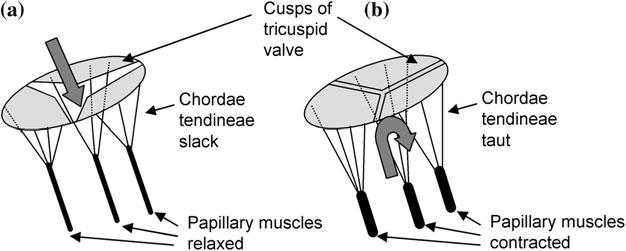
\includegraphics[width=0.8\textwidth]{88.png}
  \caption{Esquema del flujo unidireccional de una válvula cardíaca auriculoventricular. a) La presión en la aurícula supera a la del ventrículo correspondiente y la válvula se abre, como se muestra, con un chorro de sangre entrando rápidamente. Hacia el final de la diástole, el chorro se interrumpe. La desaceleración de la sangre crea una presión que tiende a cerrar la válvula. b) La válvula está normalmente cerrada (Basado en [66]).}
  \label{fig:88}
\end{figure}



El sistema sistémico fetal incluye el flujo de regreso a través del cordón umbilical y la placenta. Una vena pasa a través del cordón umbilical transportando sangre que ha pasado a través de la placenta para oxigenarse y enriquecerse con nutrientes, y se divide en el feto en un vaso que va al hígado y un segundo (el conducto venoso o *ductus venosus*) que fluye hacia la vena cava inferior. Dos arterias se ramifican de las arterias ilíacas internas, transportando sangre desoxigenada y agotada en nutrientes de regreso a través del cordón umbilical y hacia la placenta. (Al igual que en el sistema pulmonar, la sangre en estas arterias fetales (desde el corazón) está desoxigenada y la de estas venas fetales (hacia el corazón) está oxigenada).

En la madre, el flujo desde las arterias espirales (${\sim}0{,}6\text{ L/min}$) de las arterias uterinas ingresa a los espacios intervellosos de la placenta para permitir el intercambio de oxígeno, dióxido de carbono, nutrientes y desechos por difusión (pero no flujo directo) entre la sangre materna y las venas y arterias umbilicales. La sangre materna en estos espacios se intercambia $2\text{--}3\text{ veces/min}$, regresando a la madre a través de las venas uterinas. Debido a este flujo, el volumen del flujo sanguíneo materno y el gasto cardíaco aumentan durante el embarazo.

\subsection{Ciclo cardíaco}

Existe un ciclo de sincronización altamente controlado en corazones que funcionan bien, el ciclo cardíaco, el cual dura un tiempo $\tau$ (Fig.~8.5). En la primera etapa de la diástole, las venas llenan tanto la aurícula derecha como la izquierda, mientras que los ventrículos derecho e izquierdo están relajados. En la segunda etapa, el músculo cardíaco (miocardio) de las aurículas derecha e izquierda se contrae y bombea sangre a través de las válvulas auriculoventriculares hacia los ventrículos derecho e izquierdo, respectivamente, al mismo tiempo $t = 0$. (Esto es en realidad una gran simplificación del llenado ventricular, debido a que el ${\sim}75\%$ de esta sangre fluye hacia los ventrículos desde las aurículas antes de la contracción auricular). En el primer paso de la sístole, ambos ventrículos se contraen (isovolumétricamente) al mismo tiempo $\Delta$. En la segunda etapa, eyectan sangre a través de las respectivas válvulas semilunares: el ventrículo derecho hacia las arterias pulmonares y el ventrículo izquierdo hacia la aorta. La presión arterial sistólica ocurre en esta segunda etapa de la sístole, mientras que la presión diastólica es la que se presenta durante la diástole. (Una forma de medir el flujo de sangre eyectado por el ventrículo izquierdo es la balistocardiografía, la cual se describe en el Problema~8.51. Otro método es la ecocardiografía de ultrasonido Doppler, que se utiliza con más frecuencia clínicamente; se describe en el Problema~10.23).

\begin{figure}[htbp]
  \centering
  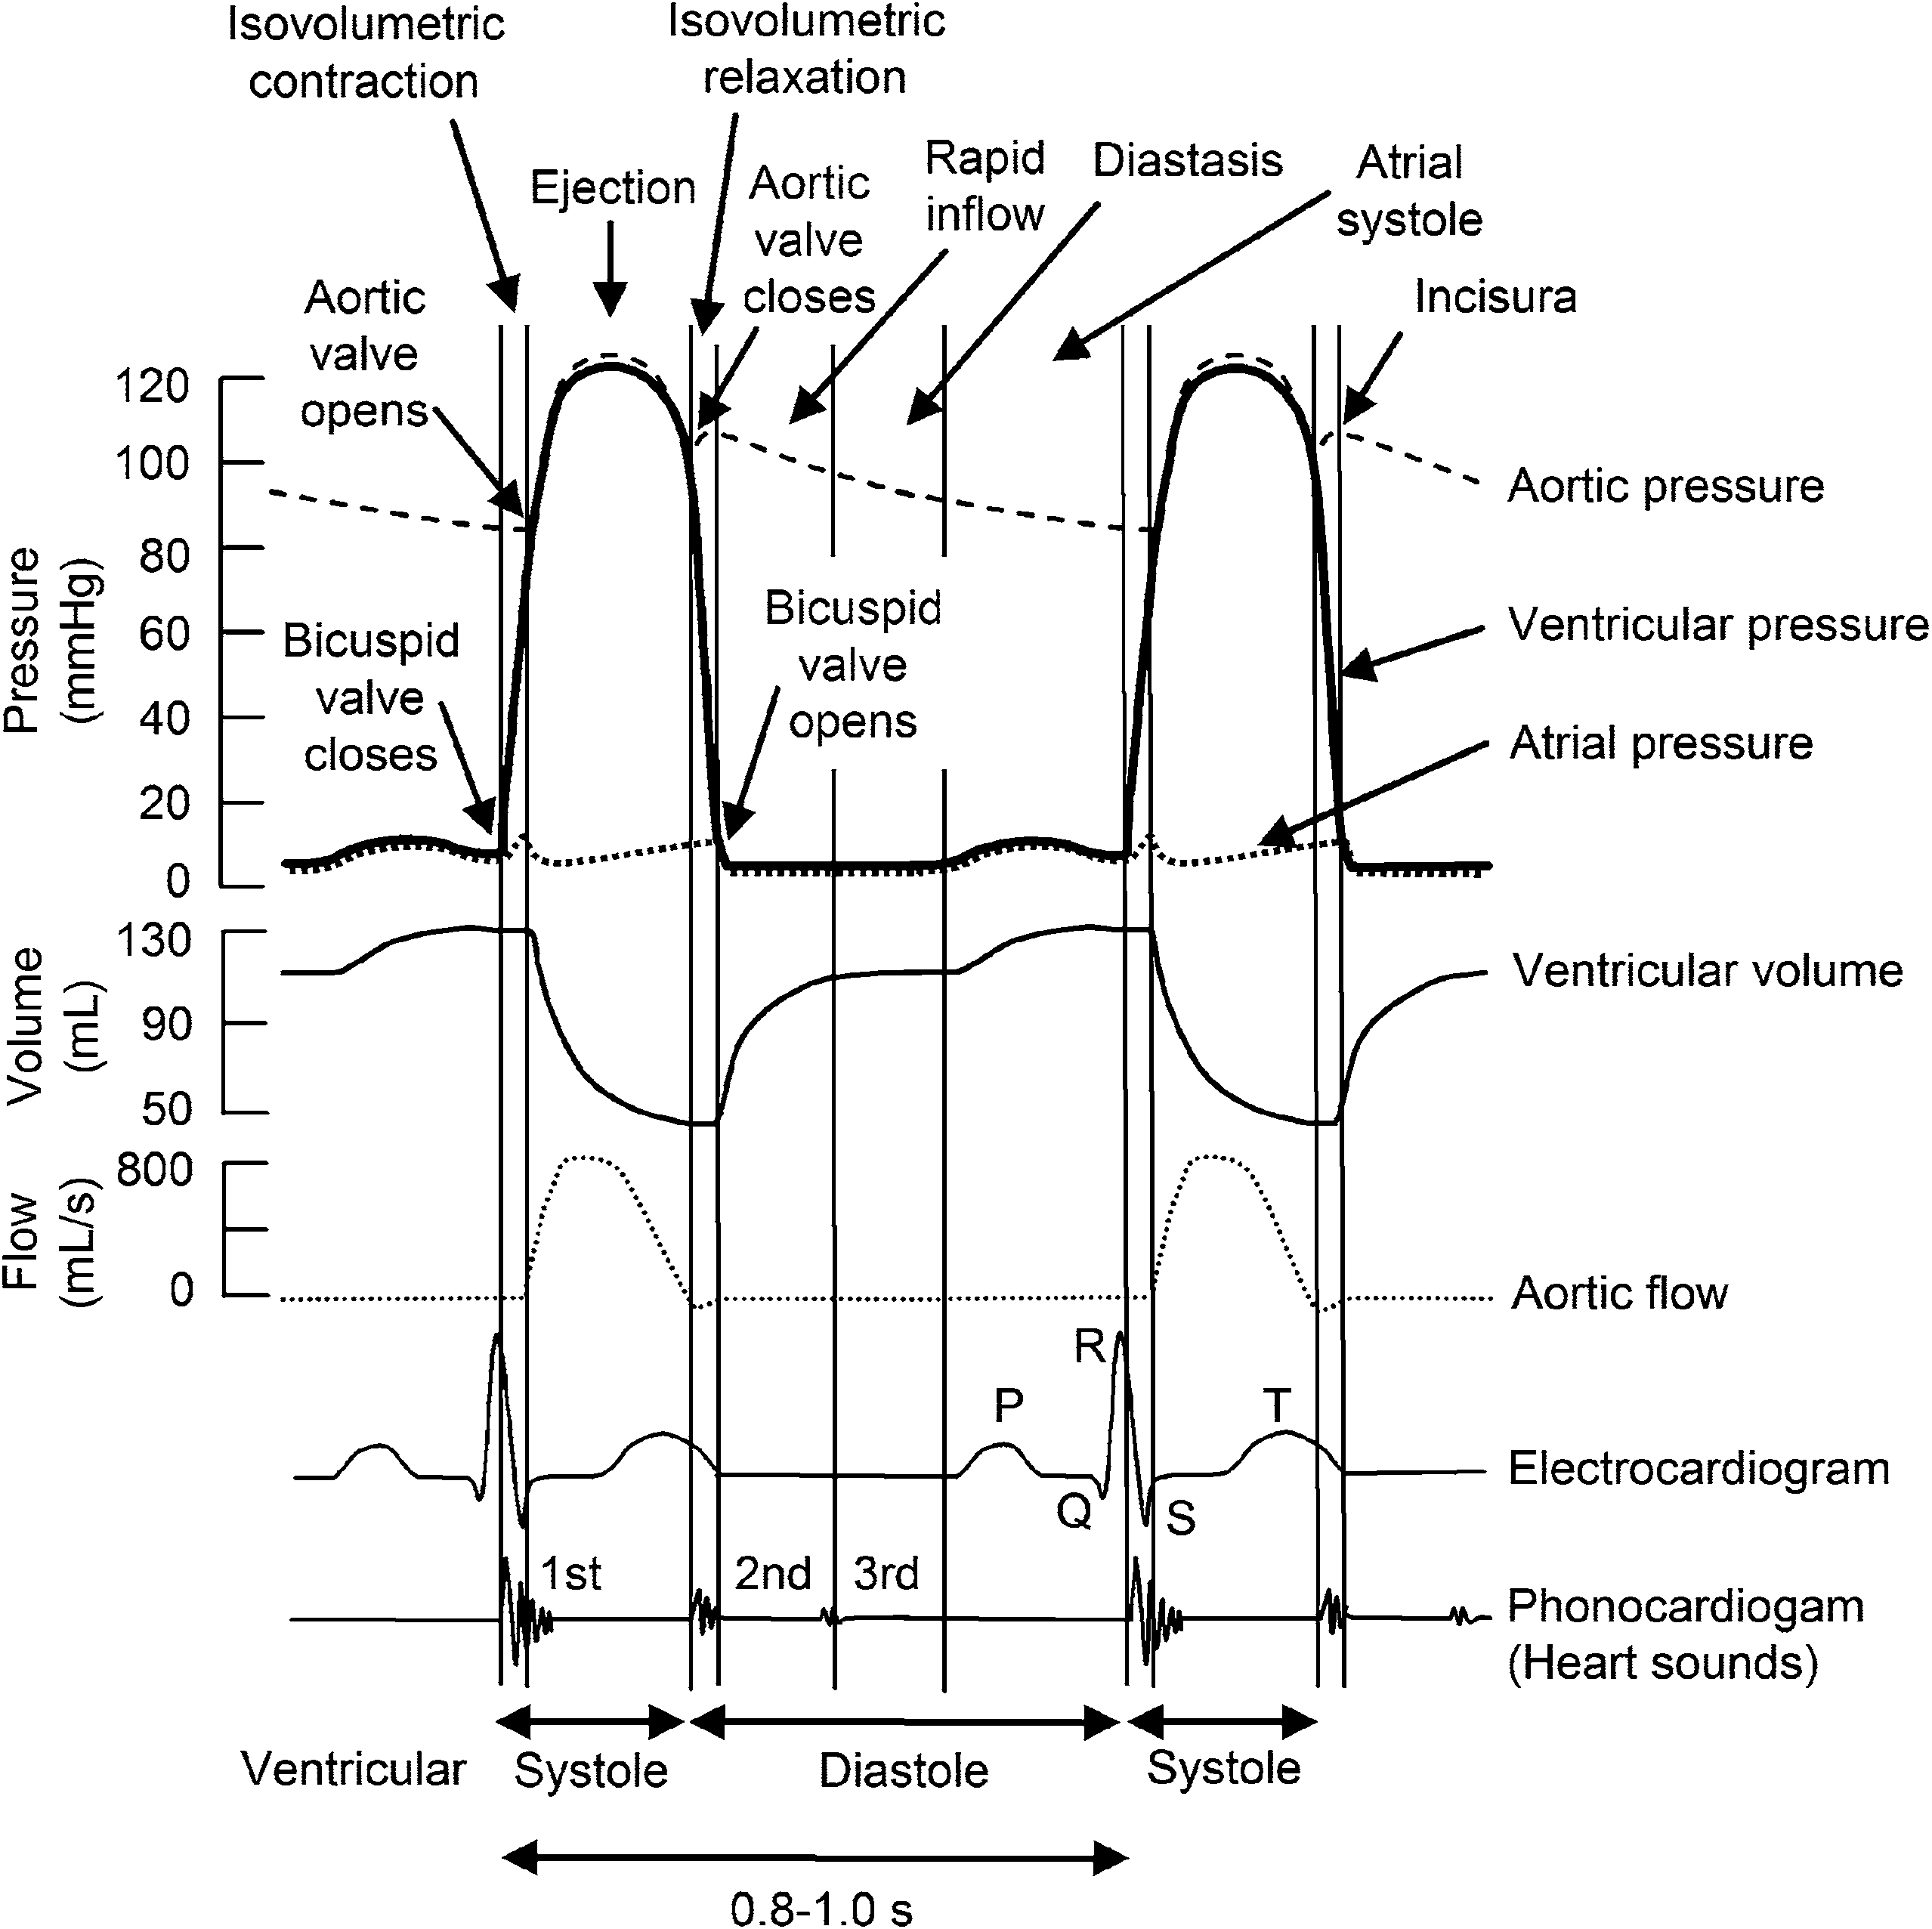
\includegraphics[width=0.55\textwidth]{85.png}
  \caption{Las presiones ventricular izquierda y auricular se trazan junto con el volumen ventricular izquierdo, la presión y el caudal aórticos, el electrocardiograma y el fonocardiograma (que es la señal de los sonidos cardíacos) en este diagrama de Wiggers. También se muestran los tiempos de apertura y cierre de las válvulas semilunar aórtica y bicúspide (mitral) (Basado en [29, 63, 66]).}
  \label{fig:85}
\end{figure}

\begin{figure}[htbp]
  \centering
  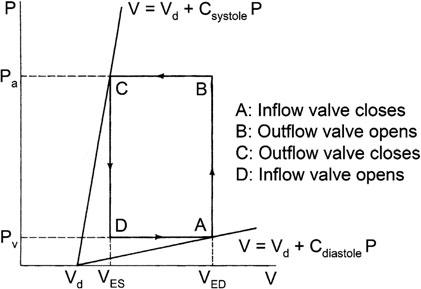
\includegraphics[width=0.7\textwidth]{851.png}
  \caption{El ciclo de presión y volumen en cualquiera de los ventrículos está representado por el rectángulo ABCD en este modelo simplificado. Las líneas inclinadas que irradian desde el volumen muerto son las relaciones de presión-volumen del ventrículo al final de la sístole y de la diástole. (Otras líneas inclinadas similares con pendientes diferentes (no mostradas) caracterizan al ventrículo en otros momentos). La presión venosa es la misma que las presiones auricular y venosa de entrada durante la diástole. La presión arterial es la presión de salida del ventrículo durante la sístole. Para el ventrículo izquierdo, $P_{\text{a}}$ es $P_{\text{sa}}$ y $P_{\text{v}}$ es $P_{\text{pv}}$; para el ventrículo derecho, $P_{\text{a}}$ es $P_{\text{pa}}$ y $P_{\text{v}}$ es $P_{\text{sv}}$ (De [34]).}
  \label{fig:851}
\end{figure}



Los corazones derecho e izquierdo deben funcionar exactamente al mismo tiempo para mantener el caudal $Q$ igual en ambos sistemas. Existe un mecanismo de sincronización para hacer esto y establecer los tiempos de contracción $0$ y $\Delta$ para un latido, seguidos de $\tau$ y $\tau + \Delta$ para el siguiente, $2\tau$ y $2\tau + \Delta$ para el siguiente, y así sucesivamente. Hay un marcapasos cardíaco en el nodo sinoauricular o sinusal (véase el sistema de conducción en la Fig.~8.6), el cual envía una señal eléctrica al músculo cardíaco auricular de ambas aurículas para la contracción auricular simultánea. Esta señal eléctrica luego viaja al nodo auriculoventricular o AV, se retrasa allí durante un tiempo $\Delta$, y luego el nodo envía una señal al músculo cardíaco ventricular de ambos ventrículos para la contracción ventricular simultánea.

\begin{figure}[htbp]
  \centering
  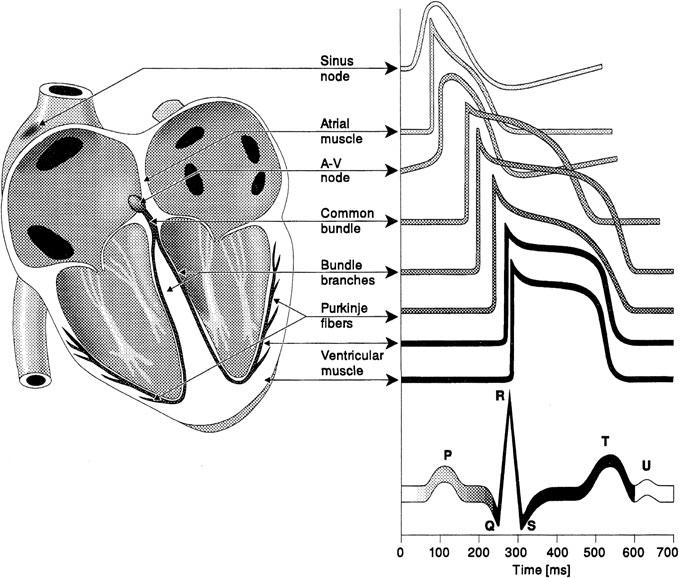
\includegraphics[width=0.7\textwidth]{86.png}
  \caption{Sistema de conducción del corazón con los nodos sinoauricular/sinusal y auriculoventricular/AV, junto con las formas de onda eléctricas de la actividad de cada uno, incluyendo el EKG en la parte inferior. Véase también la Fig.~12.28 (De [49]).}
  \label{fig:86}
\end{figure}



El electrocardiograma (EKG o ECG) es una medición de estas señales eléctricas y su sincronización, medidas por sondas en el cuerpo [17, 25, 45]. La Figura~8.6 muestra el EKG durante un latido cardíaco de ${\sim}1\text{ s}$ de duración (véase también la Fig. 12.28). La onda P se debe a la despolarización auricular (que es la contracción auricular). El complejo QRS se debe a la despolarización ventricular (contracción). La onda T se debe a la repolarización ventricular (relajación). La señal de repolarización auricular (relajación) está enmascarada por el complejo QRS más grande. La despolarización y repolarización, las propiedades eléctricas del corazón y el uso de los EKG se analizan más en el Cap.~12.

Existen varias arritmias cardíacas (es decir, irregularidades en la sincronización) de diversos niveles de preocupación que afectan a este mecanismo de sincronización cardíaca. En un bloqueo auriculoventricular, existe una lesión en las fibras auriculoventriculares (AV) desde el nodo AV hasta el ventrículo o en el propio nodo AV (Fig.~8.6). En un bloqueo AV incompleto, el tiempo de conducción a través de la unión AV aumenta desde el valor normal de $0{,}16\text{ s}$ a $0{,}25\text{--}0{,}50\text{ s}$ y ocurren latidos ventriculares omitidos; estos a veces conducen a ritmos $2:1$, $3:2$ o $3:1$ de latidos auriculares a ventriculares. En un bloqueo AV completo, una persona puede desmayarse hasta que se desarrollen latidos ventriculares (con $40\text{ /min}$, en comparación con $100\text{ latidos/min}$ en las aurículas). También pueden ocurrir contracciones prematuras de las aurículas o de los ventrículos. En la taquicardia paroxística, ocurren aumentos repentinos en la frecuencia cardíaca, digamos de $95$ a $150\text{ latidos/min}$ en las aurículas o los ventrículos, lo cual puede causar un daño ventricular (no auricular) grave. La fibrilación ventricular es la arritmia más grave y es mortal si no se trata de inmediato. Puede ser causada por corriente alterna (CA) de $60\text{ ciclos}$. Ocurre una contracción muscular descoordinada de los ventrículos, por lo que partes de ellos se contraen mientras otras partes se relajan; esto conduce a un bombeo de sangre escaso o nulo. La pérdida del conocimiento ocurre en $4\text{--}5\text{ s}$ y la muerte de los tejidos comienza en unos pocos minutos. La fibrilación auricular implica una contracción muscular descoordinada similar, pero es menos grave debido a que la mayor parte de la sangre fluye pasivamente desde las aurículas hacia los ventrículos. El flujo de sangre disminuye en solo ${\sim}20\text{--}30\%$. La reanimación después de un paro cardíaco puede ocurrir en muchos casos mediante reanimación cardiopulmonar (RCP) [29].

El músculo cardíaco es similar al músculo esquelético descrito en el Cap.~5 (Fig.~5.1b). En particular, la unidad estructural básica es el sarcómero con sus filamentos deslizantes de actina y miosina. Sin embargo, existen algunas diferencias. A la longitud de reposo del músculo, la tensión máxima para el músculo esquelético es de ${\sim}20\text{ N/cm}^2$ o más, mientras que es de solo ${\sim}7\text{ N/cm}^2$ para el músculo cardíaco. Además, la tensión pasiva en reposo es bastante grande (y relativamente mayor) a la longitud de tensión máxima en el músculo cardíaco (como se representa en la Fig.~5.21a). Ambas diferencias pueden atribuirse en parte a la mayor fracción de tejido no contráctil en el músculo cardíaco, el cual contiene colágeno y otro tejido fibrótico. La primera diferencia también surge de la naturaleza no paralela de las fibras del músculo cardíaco. Otra diferencia entre el músculo esquelético y el cardíaco es que usualmente no es posible tetanizar el músculo cardíaco. Las sacudidas se fusionan solo parcialmente a una frecuencia de estimulación muy alta.

\subsection{Válvulas}

Existen cuatro válvulas principales en el corazón (Fig.~8.7). La válvula auriculoventricular derecha controla el flujo entre la aurícula derecha y el ventrículo derecho. Tiene tres aletas (o cúspides) y por lo tanto también se le llama válvula tricúspide. La válvula semilunar pulmonar controla el flujo de sangre desde el ventrículo derecho hacia las arterias pulmonares izquierda y derecha. La válvula auriculoventricular izquierda controla el flujo desde la aurícula izquierda hacia el ventrículo izquierdo. Tiene dos aletas y por lo tanto también se le llama válvula bicúspide. Otro nombre para esta válvula es la válvula mitral, debido a que se parece a una mitra. La válvula semilunar aórtica controla el flujo desde el ventrículo izquierdo hacia la aorta.

\begin{figure}[htbp]
  \centering
  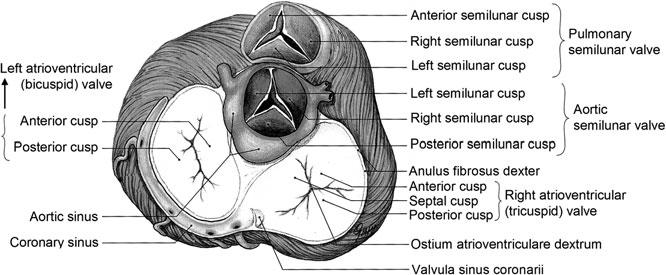
\includegraphics[width=0.8\textwidth]{87.png}
  \caption{Dibujo de las cuatro válvulas principales del corazón, mostrando las cúspides (aletas) (De [68]).}
  \label{fig:87}
\end{figure}



Estas cuatro válvulas comparten algunas características comunes. Son válvulas unidireccionales (Fig.~8.8) que permiten el flujo de sangre en la dirección descrita bajo algunas condiciones, pero nunca en la dirección opuesta (a menos que sean defectuosas). Podemos imaginar una válvula unidireccional con aletas que no permita ningún flujo de retorno. Con este tipo de válvula podemos ver cómo se abrirán las aletas, permitiendo este flujo unidireccional, cuando la presión delante de la válvula supere a la del otro lado. De esta manera, la válvula permanece cerrada hasta que la presión en la cavidad aumente debido a la contracción a un valor mayor que el que hay después de la válvula. Sin embargo, tal válvula no puede soportar mucha contrapresión. La apertura hacia atrás de las válvulas auriculoventriculares también se evita mediante los músculos papilares en el lado ventricular, los cuales se contraen cuando la válvula está cerrada, tensando las cuerdas tendinosas que están unidas a las aletas (Fig.~8.9). Esto evita que las aletas se doblen hacia atrás, por lo que no hay flujo retrógrado de sangre.

\begin{figure}[htbp]
  \centering
  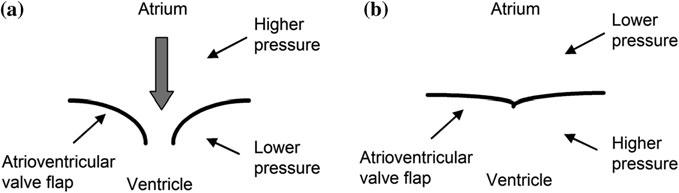
\includegraphics[width=0.8\textwidth]{89.png}
  \caption{Los músculos papilares en el lado ventricular de las válvulas auriculoventriculares se contraen cuando las válvulas están cerradas, tensando las cuerdas tendinosas y evitando el flujo retrógrado, como en b). Los músculos y las cuerdas tendinosas están relajados cuando las válvulas están abiertas y se permite el flujo de sangre hacia adelante, como en a) (Basado en [66]).}
  \label{fig:89}
\end{figure}



Consideremos el ciclo para la válvula semilunar aórtica. Durante la relajación ventricular, la presión en el ventrículo izquierdo es de ${\sim}0\text{ mmHg}$. En la aorta, la presión es de ${\sim}120\text{ mmHg}$ durante la sístole y luego disminuye a ${\sim}80\text{ mmHg}$ durante la diástole, justo antes de la contracción ventricular. La válvula permanece cerrada. Durante la contracción ventricular, la presión en el VI aumenta a $80\text{ mmHg}$, continuando hasta ${\sim}120\text{ mmHg}$. Debido a que la presión en la aorta es de ${\sim}80\text{ mmHg}$, la válvula semilunar aórtica se abre una vez que la presión en el VI supera los $80\text{ mmHg}$ y luego permanece abierta. Durante este flujo, la presión en el VI y en la aorta se iguala, ${\sim}120\text{ mmHg}$, y luego la válvula se cierra a medida que el ciclo de flujo llega a su fin.

La medición de las presiones sistólica y diastólica mediante la escucha de los sonidos de Korotkoff se describe en el Cap.~7. Este método es la forma estándar de determinar la presión arterial a pesar de que habitualmente subestima la presión sistólica en $5\text{--}20\text{ mmHg}$ y sobreestima la presión diastólica en $12\text{--}20\text{ mmHg}$ [15]. (Tiene la precisión necesaria para un diagnóstico, a pesar de que no es muy exacto).

Las aperturas y cierres de las válvulas cardíacas y el flujo de sangre en el corazón crean sonidos que pueden escucharse con un estetoscopio, y se describen en el Cap.~10. (Véase también la Fig.~8.5). La ecocardiografía es el uso de ultrasonido para diagnosticar trastornos cardíacos y flujos sanguíneos. Este y otros métodos relacionados también se describen brevemente en el Cap.~10 (y en los Problemas 10.22 y 10.23).

\section{Física del sistema circulatorio}

Ahora examinamos el sistema circulatorio con mayor detalle. Primero, examinaremos cómo varía la presión arterial con la distancia a lo largo de las arterias y venas, incluyendo dentro de los capilares. Luego investigaremos las consecuencias de las falta de uniformidad en las arterias, tales como arterias obstruidas y aneurismas, en el contexto de la resistencia de las paredes arteriales. A continuación, calcularemos el trabajo realizado por el corazón, para ver cómo este contribuye a las necesidades metabólicas del cuerpo. En la última sección de este capítulo, desarrollaremos un modelo de todo el sistema circulatorio y del corazón.

\subsection{Propiedades de la sangre}

La sangre es un fluido no newtoniano, en parte debido a su composición compleja y heterogénea [40]. La solución sanguínea consta de plasma, glóbulos rojos (eritrocitos; $5\text{ millones/mm}^3$; $45\%$ del volumen total de sangre), glóbulos blancos (leucocitos; $0{,}3\%$) y plaquetas ($0{,}15\%$). (La fracción de volumen de los glóbulos rojos se denomina hematocrito). Los glóbulos rojos son discos bicóncavos que tienen forma toroidal con el centro parcialmente relleno, y tienen un diámetro de $7{,}5\text{ }\mu\text{m}$ y un espesor máximo de $2\text{ }\mu\text{m}$. Su diámetro es aproximadamente el mismo que el diámetro interno de los capilares, pero pueden deformarse y fluir en tubos aún más pequeños. Los glóbulos blancos son esféricos, con un diámetro de $7\text{ }\mu\text{m}$, mientras que las plaquetas son mucho más pequeñas. El plasma sanguíneo es $90\%$ agua y se comporta como un fluido newtoniano con una viscosidad de $0{,}0012\text{ Pa}\cdot\text{s}$. La reología de la sangre se ve alterada en gran medida por los glóbulos rojos, y no mucho por los glóbulos blancos o las plaquetas debido a que estos constituyen fracciones muy pequeñas del volumen sanguíneo. (La reología es el estudio de la deformación y el flujo de los materiales, en particular de materiales inusuales). La viscosidad de la sangre aumenta con el hematocrito, como se ve en la Fig.~8.10.

\begin{figure}[htbp]
  \centering
  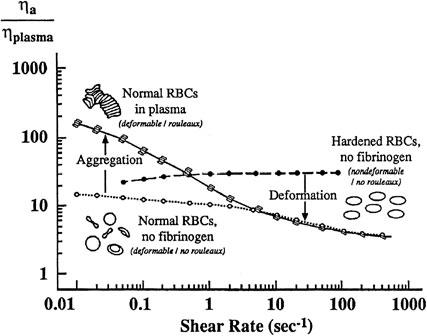
\includegraphics[width=0.7\textwidth]{810.png}
  \caption{Viscosidad de la sangre en función del hematocrito (Basado en [29]).}
  \label{fig:810}
\end{figure}



La viscosidad efectiva de la sangre disminuye a medida que aumenta la tasa de cizallamiento (Fig.~8.11). Para tasas de cizallamiento muy bajas, esta viscosidad es más de $100$ veces la del agua, mientras que a las altas tasas de cizallamiento características del flujo en vasos más grandes es de aproximadamente $4$ veces la del agua, con un valor de $0{,}004\text{--}0{,}005\text{ Pa}\cdot\text{s}$.

\begin{SCfigure}[0.8][htbp]
  \centering
  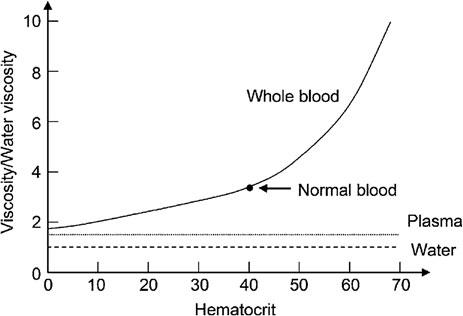
\includegraphics[width=0.55\textwidth]{811.png}
  \caption{Viscosidad de la sangre en función de la tasa de cizallamiento para un hematocrito del $45\%$, a $310\text{ K}$ (De [21]. Cortesía de Robert A. Freitas Jr., Nanomedicine, Vol. 1 (1999), http://www.nanomedicine.com, basado en [13]).}
  \label{fig:811}
\end{SCfigure}



La viscosidad de algunos fluidos cambia incluso mientras la tasa de deformación es constante. La sangre es un fluido tixotrópico, para el cual el esfuerzo cortante disminuye mientras la tasa de deformación es constante. Aún así, para nuestros propósitos será adecuado tratar la sangre como un fluido newtoniano, a pesar de que el perfil de velocidad del flujo no tiene la forma parabólica ideal para un fluido newtoniano (Fig.~7.13).

\subsection{Presión sanguínea y flujo en los vasos}

\subsubsection*{Estructura de los vasos sanguíneos}

Las paredes de las arteriolas contienen menos tejido elástico y más músculos lisos, y se estiran relativamente poco. Las paredes de los capilares están compuestas por una sola capa de células endoteliales. Los diámetros de los capilares son tan pequeños que los glóbulos rojos apenas pueden pasar a través de ellos.

\begin{figure}[htbp]
  \centering
  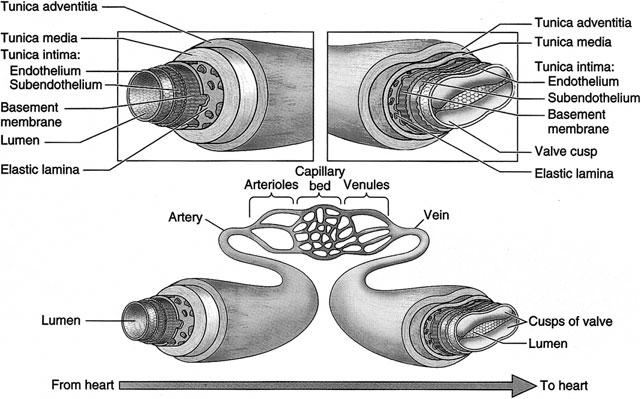
\includegraphics[width=0.8\textwidth]{812.png}
  \caption{Esquema de las paredes de arterias y venas (De [53]. Usado con permiso).}
  \label{fig:812}
\end{figure}



Aproximadamente el $70\%$ de las paredes de arterias y venas está compuesto de agua, la cual no es elástica, excepto en la forma en que soporta la compresión. El otro $30\%$ consiste en la masa seca: elastina, colágeno y fibras de músculo liso, cada uno con diferentes propiedades de materiales. Como se analizó en el Cap.~4, la elastina es similar a la goma y tiene un módulo de Young de ${\sim}3 \times 10^5\text{ Pa}$; puede estirarse hasta el doble de su longitud relajada. El colágeno es mucho más rígido, con un módulo de Young de ${\sim}1 \times 10^8\text{ Pa}$. La elastina tiene un esfuerzo de tracción último (UTS) menor al $5\%$ del del colágeno. El músculo liso tiene un módulo de Young más parecido al de la elastina, con $Y \sim 1 \times 10^5\text{ Pa}$ cuando está relajado y ${\sim}2 \times 10^6\text{ Pa}$ cuando está activo. Alrededor de la mitad de la masa seca en los vasos es elastina y colágeno, con más elastina que colágeno en la aorta (${\sim}1{,}5\times$) y relativamente menos elastina en otras arterias (${\sim}0{,}5\times$) y venas (${\sim}0{,}3\times$). Las venas contienen menos elastina que las arterias. La fracción de músculo liso en la masa seca promedia un ${\sim}50\%$, y es del ${\sim}25\%$ en la aorta, e incrementa a un ${\sim}60\%$ de manera más periférica en las arterias y arteriolas. Las propiedades mecánicas de estos vasos (Cap.~4) también dependen del tejido al cual están unidos. Esto es particularmente significativo para los capilares, debido a que las paredes de los vasos son esencialmente una sola capa de células endoteliales.

\subsubsection*{Presión sanguínea}

Se necesita presión sanguínea para impulsar el flujo de sangre. La Figura~8.13 es un esquema de la presión sanguínea arterial y venosa media en diferentes posiciones del ciclo circulatorio, para una persona acostada horizontalmente. Las oscilaciones en la presión sanguínea a lo largo de las arterias principales en la circulación sistémica reflejan la presión oscilante de esta sangre a medida que sale de la aorta, a presiones entre ${\sim}80\text{ mmHg}$ ($P_{\text{diastole}}$, en la diástole) y ${\sim}120\text{ mmHg}$ ($P_{\text{systole}}$, en la sístole) (Fig.~8.13). Debido a que la sístole dura aproximadamente $1/3$ del ciclo y la diástole aproximadamente $2/3$, la presión sanguínea media es una suma ponderada,
\begin{equation}
P_{\text{mean}} = \frac{P_{\text{systole}} + 2P_{\text{diastole}}}{3},
\label{eq:81}
\end{equation}

\begin{figure}[htbp]
  \centering
  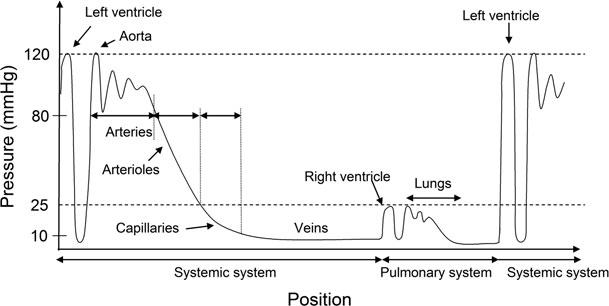
\includegraphics[width=0.8\textwidth]{813.png}
  \caption{Presión sanguínea a lo largo del sistema circulatorio para una persona acostada horizontalmente (Basado en [9]).}
  \label{fig:813}
\end{figure}



o $(1/3)120\text{ mmHg} + (2/3)80\text{ mmHg} \sim 94\text{ mmHg}$ en este ejemplo. Esta diferencia de presión de $40\text{ mmHg}$ entre la sístole y la diástole es la presión de pulso arterial $P_{\text{pulse}}$. Veremos que la sangre fluye a una velocidad de ${\sim}20\text{ cm/s}$ en estas arterias sistémicas, por lo que con una frecuencia cardíaca de aproximadamente $1\text{ Hz} = 1\text{ ciclo/s}$ es razonable que existan variaciones de presión cuasiperiódicas aproximadamente cada $20\text{ cm}$ o menos. Gran parte de la caída de presión en el sistema arterial ocurre en las arteriolas (arterias pequeñas) y los capilares. Veremos que esto puede atribuirse al flujo viscoso. En las venas hay una presión muy baja. Es una presión demasiado baja para bombear la sangre de regreso al corazón, incluso con los grandes diámetros de las venas y, por consiguiente, la baja resistencia al flujo (7.24). Existe un mecanismo de bombeo peristáltico por parte de los músculos que rodean las venas grandes que ayuda al retorno de la sangre venosa al corazón, con válvulas unidireccionales para evitar el reflujo (Fig.~8.14). (De manera similar, el flujo de sangre en los capilares usualmente no es continuo, sino que se activa y desactiva cada pocos segundos o minutos, debido a los músculos esfínteres que pueden contraer las arteriolas alimentadoras (vasomoción)). El sistema pulmonar refleja esta circulación sistémica, excepto que las presiones son todas más bajas. Las Figuras~8.13, 8.15 y 8.16 muestran la presión sanguínea y la velocidad de flujo en diferentes puntos del árbol arterial.

\begin{figure}[htbp]
  \centering
  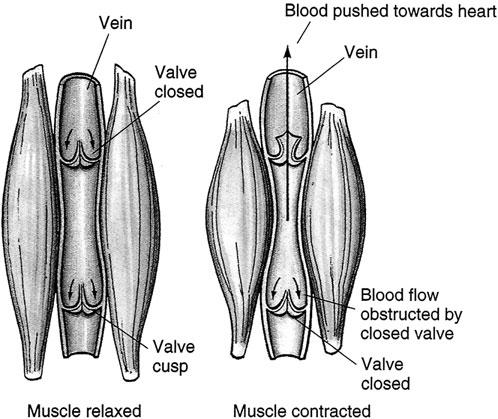
\includegraphics[width=0.7\textwidth]{814.png}
  \caption{Bomba musculovenosa de las venas, con la expansión hacia afuera de los vientres de los músculos que se contraen bombeando la sangre de regreso al corazón contra la gravedad y el cierre de las válvulas distales para evitar el reflujo (De [53]. Usado con permiso).}
  \label{fig:814}
\end{figure}

\begin{figure}[htbp]
  \centering
  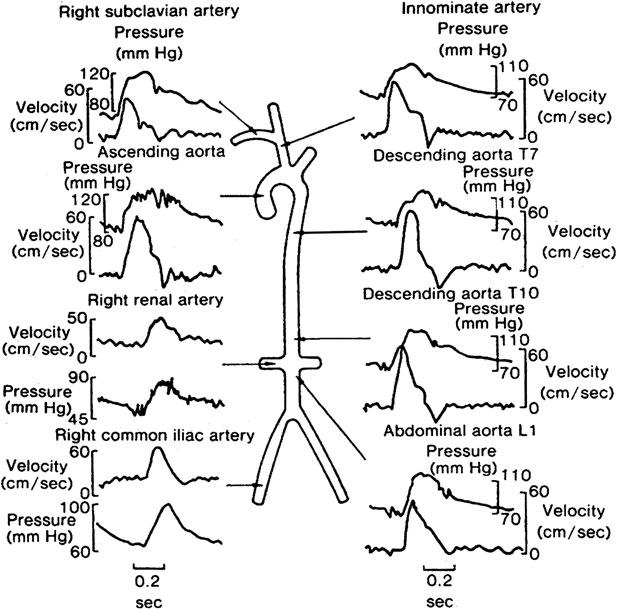
\includegraphics[width=0.55\textwidth]{815.png}
  \caption{Presión y velocidad de flujo simultáneas en diferentes puntos del árbol arterial humano para una persona acostada horizontalmente. Todos los datos fueron tomados de un solo paciente, excepto para la arteria renal derecha y la arteria ilíaca común derecha (De [31]. Adaptado de [52]).}
  \label{fig:815}
\end{figure}

\begin{figure}[htbp]
  \centering
  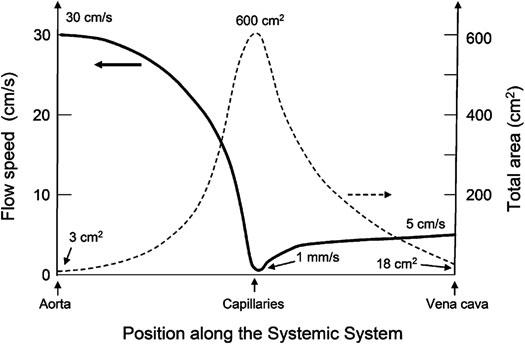
\includegraphics[width=0.7\textwidth]{816.png}
  \caption{Velocidad de flujo (curva sólida) y área total (curva discontinua) en el sistema de circulación sistémica (Basado en [9]).}
  \label{fig:816}
\end{figure}



El ciclo de bombeo establece una onda de pulso de presión además de la variación de la presión hidrostática. La velocidad de esta onda de pulso es independiente de la velocidad del flujo sanguíneo (y es más rápida que la velocidad del flujo sanguíneo) y es de $4\text{ m/s}$ en la aorta, $8\text{ m/s}$ en las arterias grandes y $16\text{ m/s}$ en las arterias pequeñas de adultos jóvenes.

Cuando se está de pie verticalmente (Fig.~8.17), hay una presión adicional $\rho g h$, donde $h$ es la altura relativa al corazón. Esta es aproximadamente la altura en la parte superior del brazo donde se realizan las mediciones de la presión arterial. Para $\rho = 1{,}06\text{ g/cm}^3 = 1\,060\text{ kg/m}^3$, $g = 9{,}8\text{ m/s}^2$ y $h = 1\text{ m}$, esta presión es de $10\,400\text{ N/m}^2 = 10\,400\text{ Pa} = 79\text{ mmHg}$ (con $1\text{ MPa} = 7\,600\text{ mmHg}$). A cualquier altura dada, la diferencia de presión impulsora desde las arterias hacia las venas no cambia. Además, este cambio de presión no es importante al considerar cambios de presión entre el interior y el exterior de un vaso porque $\rho g h$ se suma tanto dentro como fuera del vaso.

\begin{SCfigure}[0.8][htbp]
  \centering
  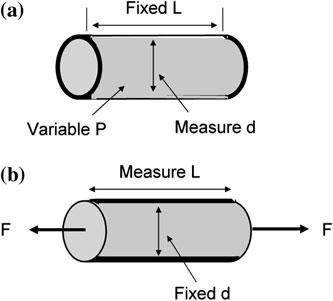
\includegraphics[width=0.55\textwidth]{817.png}
  \caption{Presiones arteriales y venosas medias (manométricas) para una persona vertical (De [10], según [61]. Usado con permiso de Oxford University Press).}
  \label{fig:817}
\end{SCfigure}



Aun así, este efecto de la gravedad puede ser significativo. La presión sanguínea en la aorta tiene que ser lo suficientemente alta como para bombear la sangre hasta la parte superior de su cerebro. Esta distancia es de aproximadamente $h = 40\text{ cm}$, por lo que la caída de presión es de aproximadamente $30\text{ mmHg}$ (en comparación con la presión diastólica de ${\sim}80\text{ mmHg}$). Los Problemas~8.1 y 8.2 exploran lo que sucede con la circulación sanguínea craneal en humanos en aviones de reacción que ascienden rápidamente y en planetas más masivos con mayor $g$, y también en jirafas. Una manifestación de este efecto de la gravedad es el desmayo potencial al ponerse de pie. Al ponerse de pie, el volumen de sangre en las venas de las piernas aumenta y la presión en las venas que bombean sangre de regreso al corazón disminuye. Esto puede disminuir el gasto cardíaco y el flujo de sangre al cerebro. Esto rara vez sucede porque hay una constricción refleja de las venas en las piernas (debido a una contracción del músculo esquelético que rodea las venas, Fig.~8.14) que limita la acumulación de sangre y una constricción arteriolar que aumenta la resistencia al flujo y aminora la disminución en la presión sanguínea arterial. El efecto de la gravedad en los humanos —quienes normalmente se paran erguidos— también explica por qué no es recomendable pararse de cabeza por períodos prolongados (Problema~8.3). Las venas en su cabeza no están diseñadas para bombear sangre de regreso al corazón (como lo están las de la parte inferior del cuerpo). Además, sus pies dejarían de recibir sangre. También explica por qué las venas varicosas empeoran al estar de pie erguido, porque la sangre entonces necesita ser bombeada hacia arriba.

El control corporal de la presión sanguínea se describe brevemente en el Cap.~13.

\subsubsection*{Medición del flujo en los vasos sanguíneos}

Las propiedades mecánicas de los vasos sanguíneos se pueden medir bajo dos tipos de condiciones. (1) La longitud de un vaso dado se puede mantener constante, mientras que su diámetro se mide en función de la presión de distensión. Esto conduce a un esfuerzo de tracción en la pared, dirigido alrededor de la circunferencia, el cual se denomina esfuerzo circunferencial o de aro. (2) El diámetro de un vaso se puede mantener constante, mientras que su longitud se mide a medida que se estira longitudinalmente. En la Fig.~8.18 se muestran ejemplos de ambos.

\begin{SCfigure}[1.3][htbp]
  \centering
  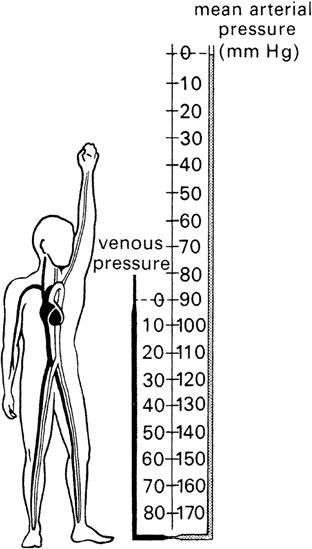
\includegraphics[width=0.35\textwidth]{818.png}
  \caption{Medición de las propiedades mecánicas de los vasos sanguíneos fijando el vaso en a) su longitud (lo cual se denomina inflación) o b) su diámetro (lo cual se denomina extensión). Algunos investigadores realizan cargas combinadas, con combinaciones de inflación, extensión y torsión.}
  \label{fig:818}
\end{SCfigure}



El flujo de sangre en las arterias se ve afectado por cambios en la frecuencia de los latidos cardíacos y en el volumen sistólico (el cual es el volumen bombeado por latido), y también por cambios en las arterias mismas que controlan sus diámetros mediante mecanismos químicos y neuronales.

\subsubsection*{Modelado del flujo en los vasos sanguíneos}

La Figura~8.19 es un esquema que describe el flujo en un vaso de longitud $L$, con un caudal volumétrico de entrada $Q_1$ y de salida $Q_2$. En estado estacionario $Q_1 = Q_2 = Q$, el cual se promedia sobre un latido cardíaco. Al inicio del vaso la presión es $P_1$ y al final es $P_2$. La presión fuera del vaso es $P_{\text{ext}}$, la cual se puede tomar como $0$ cuando se utiliza la presión manométrica. El volumen del vaso es $V$. La relación entre estos diversos parámetros depende de las propiedades de los vasos.

\begin{SCfigure}[0.75][htbp]
  \centering
  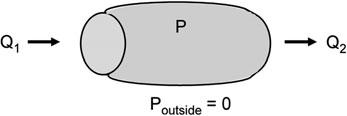
\includegraphics[width=0.6\textwidth]{819.png}
  \caption{Flujo sanguíneo: vaso general.}
  \label{fig:819}
\end{SCfigure}



Existen dos atributos físicos de los vasos sanguíneos en estado estacionario. (a) Tienen una resistencia al flujo, por lo que necesitan una diferencia de presión a lo largo de la longitud del vaso para impulsar el flujo sanguíneo. (b) Tienen una compliancia en respuesta a una presión de distensión. Esto es muy parecido a un globo que se expande cuando la presión en su interior aumenta muy por encima de la del exterior.

Un caso especial es un vaso rígido con volumen $V$ constante, el cual se denomina vaso de resistencia (Fig.~8.20). La ecuación~(8.2) se aplica a este vaso, por lo que
\begin{equation}
P_1 - P_2 = R_{\text{flow}} Q
\label{eq:82}
\end{equation}
o
\begin{equation}
Q = \frac{1}{R_{\text{flow}}} (P_1 - P_2),
\label{eq:83}
\end{equation}
donde la resistencia vascular es $R_{\text{flow}} = 8\eta L/\pi r^4$ para un tubo con radio $r$. La primera ecuación tiene la misma forma que la ley de Ohm $V_{\text{elect},1} - V_{\text{elect},2} = R_{\text{elect}} I$, la cual relaciona la caída de voltaje, $V_{\text{elect}}$, cuando una corriente de cargas $I$ atraviesa una estructura con resistencia eléctrica $R_{\text{elect}}$.

\begin{SCfigure}[0.75][htbp]
  \centering
  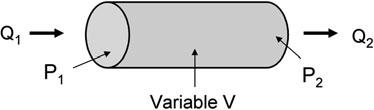
\includegraphics[width=0.6\textwidth]{820.png}
  \caption{Flujo sanguíneo: vaso de resistencia ideal.}
  \label{fig:820}
\end{SCfigure}



Un segundo caso especial es un vaso elástico que no tiene una resistencia apreciable, el cual se denomina vaso de compliancia. No hay caída de presión, por lo que $P_1 = P_2 = P$. Un modelo (Fig.~8.21) de las propiedades de tal vaso es
\begin{equation}
V(P) = C_{\text{flow}} (P - P_{\text{ext}}) = C_{\text{flow}} P,
\label{eq:84}
\end{equation}

\begin{SCfigure}[0.75][htbp]
  \centering
  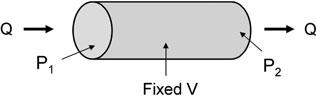
\includegraphics[width=0.6\textwidth]{821.png}
  \caption{Flujo sanguíneo: vaso de compliancia ideal.}
  \label{fig:821}
\end{SCfigure}



donde $C_{\text{flow}}$ es la compliancia y $P_{\text{ext}}$ se toma como $0$. Debido a que el vaso usualmente tiene un volumen sin presión, llamado volumen muerto $V_{\text{d}}$, una mejor relación es
\begin{equation}
V(P) = V_{\text{d}} + C_{\text{flow}} P.
\label{eq:85}
\end{equation}

Nótese que una propiedad del vaso de resistencia, a saber, el caudal, se ve afectada por la caída de presión a lo largo (e interior) del vaso, mientras que una propiedad del vaso de compliancia, su volumen, se ve afectada por la diferencia de presión entre el interior y el exterior del vaso. También podemos describir la compliancia mediante cambios en el área $A$
\begin{equation}
A(P) = A_{\text{d}} + c_{\text{flow}} P,
\label{eq:86}
\end{equation}

donde $A_{\text{d}}$ es el área sin diferencia de presión y $c_{\text{flow}}$ es la compliancia por unidad de longitud, o por cambios en el radio $r$
\begin{equation}
r(P) = r_{\text{d}} + \frac{C'_{\text{flow}}}{2} P,
\label{eq:87}
\end{equation}

donde $r_{\text{d}}$ es el radio sin diferencia de presión. Debido a que $V = A L = \pi r^2 L$ y $V_{\text{d}} = A_{\text{d}} L = \pi r_{\text{d}}^2 L$ para un vaso de radio $r$ y longitud $L$, estas formulaciones se pueden interrelacionar, con $c_{\text{flow}} = C_{\text{flow}}/L$ y $C'_{\text{flow}} = C_{\text{flow}}/\pi r L = c_{\text{flow}}/\pi r$ (siendo este último conjunto de relaciones válido para pequeños cambios en $r$ o $V$).

Los vasos reales tienen algunos atributos de ambos tipos de vasos. Aun así, la aorta, las arterias grandes y las venas grandes son muy parecidas a los vasos de compliancia. Veremos que las caídas de presión a lo largo de ellos son relativamente pequeñas. Las arteriolas, los capilares y las vénulas actúan como vasos de resistencia. Veremos que ellos, y en particular las arteriolas, son los principales sitios de la caída de presión, y esta es la razón por la cual el corazón necesita bombear sangre a presiones tan altas.

\subsubsection*{Caídas de presión en las arterias y vasos resistivos}

Utilizaremos la ley de Poiseuille $\Delta P = \left(\frac{8\eta L}{\pi r^4}\right) Q$ (7.25) para estimar la caída de presión $\Delta P = P_1 - P_2$ a través de la aorta, las arterias grandes, las arteriolas y los capilares, y compararemos estos resultados con el gráfico de la Fig.~8.13 (y véase también la Fig.~8.15). Primero calculamos la resistencia $R_{\text{flow},0} = 8\eta L_0/\pi r_0^4$ para un radio estándar $r_0 = 1\text{ cm}$ y longitud estándar $L_0 = 1\text{ cm}$, y escalamos los resultados para cada caso específico. Con la viscosidad $\eta = 4{,}0 \times 10^{-3}\text{ Pa}\cdot\text{s} = 4{,}0 \times 10^{-3}\text{ (N}\cdot\text{s/m}^2) = 4{,}0 \times 10^{-2}\text{ poise}$ para la sangre entera a $37\text{ }^\circ\text{C}$,
\begin{equation}
R_{\text{flow},0} = \frac{8 \times (4{,}0 \times 10^{-3}\text{ N}\cdot\text{s/m}^2)(1\text{ cm})}{\pi(1\text{ cm})^4} = 1{,}02 \times 10^{-2}\text{ }\frac{\text{N/m}^2}{\text{cm}^3\text{/s}}
\label{eq:88}
\end{equation}
\begin{equation}
= 1{,}02 \times 10^{-8}\text{ }\frac{\text{N/mm}^2}{\text{cm}^3\text{/s}} = 7{,}7 \times 10^{-5}\text{ }\frac{\text{mmHg}}{\text{cm}^3\text{/s}},
\label{eq:89}
\end{equation}
donde hemos utilizado $0{,}1\text{ N/mm}^2 = 1\text{ atm} \simeq 760\text{ mmHg}$. Las unidades en (8.9) son $\text{mmHg}\cdot\text{s/cm}^3$. Esta es la resistencia cuando la diferencia de presión es de $1\text{ mmHg}$ y el caudal es de $1\text{ mL/s}$, y también se conoce como una URP, una unidad de resistencia periférica. Esta unidad se utiliza comúnmente en fisiología.

La resistencia de un vaso de longitud y radio arbitrarios es
\begin{equation}
R_{\text{flow}} = R_{\text{flow},0} \frac{L/L_0}{(r/r_0)^4} = R_{\text{flow},0} \frac{L(\text{en cm})}{r(\text{en cm})^4}
\label{eq:810}
\end{equation}
y por lo tanto
\begin{equation}
\Delta P = R_{\text{flow}} Q = 7{,}7 \times 10^{-5}\text{ mmHg } \frac{L(\text{en cm})}{r(\text{en cm})^4} Q (\text{en cm}^3\text{/s}).
\label{eq:811}
\end{equation}

El caudal total, $Q_{\text{t}}$, desde la aorta, ingresa a las arterias grandes, y todo el flujo de las arterias grandes ingresa a las arteriolas, y finalmente todo este flujo ingresa a los capilares. En cada nivel de flujo modelaremos las arterias como $n$ vasos paralelos de longitud y radio aproximadamente equivalentes que transportan aproximadamente el mismo flujo (Fig.~8.22), donde $n$ aumenta para cada nivel de flujo sucesivo. Así, en un nivel de flujo dado con $n$ vasos, el caudal en cada vaso es de ${\sim}Q_{\text{t}}/n$.

\begin{SCfigure}[0.9][htbp]
  \centering
  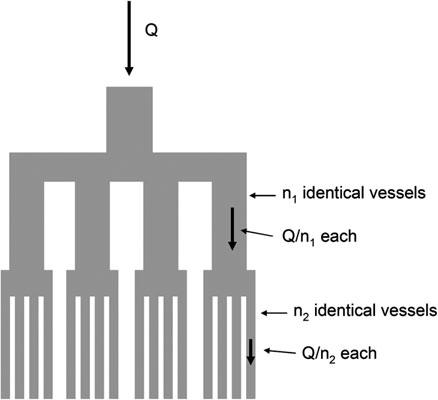
\includegraphics[width=0.5\textwidth]{822.png}
  \caption{Esquema del flujo sanguíneo en vasos ramificados idealizados.}
  \label{fig:822}
\end{SCfigure}



Con $Q_{\text{t}} = 80\text{ cm}^3\text{/s}$ y $Q = Q_{\text{t}}/n$, obtenemos
\begin{equation}
\Delta P = 7{,}7 \times 10^{-5}\text{ mmHg } \frac{L(\text{en cm})}{r(\text{en cm})^4} \frac{80}{n}
\label{eq:812}
\end{equation}
\begin{equation}
= \frac{0{,}0062\text{ mmHg}}{n} \frac{L(\text{en cm})}{r(\text{en cm})^4}.
\label{eq:813}
\end{equation}

Esta es la caída de presión a través de cualquier vaso en un nivel de flujo dado y, debido a que están en paralelo, es la caída de presión a través de todo el nivel dado de flujo arterial. Ahora determinamos esto para los diversos niveles de arterias.

Aorta. Existe una aorta ($n = 1$) con $r \sim 1{,}25\text{ cm}$ y $L \sim 10\text{ cm}$, por lo que $\Delta P$ a través de la aorta es de $0{,}025\text{ mmHg}$, lo cual es insignificante.

Arterias más grandes. Existen alrededor de $200$ arterias grandes con $r \sim 0{,}2\text{ cm}$ y $L \sim 75\text{ cm}$, por lo que $\Delta P$ es de $1{,}4\text{ mmHg}$, lo cual es bastante insignificante.

Arterias más pequeñas y arteriolas. Existen alrededor de $5 \times 10^5$ arteriolas con $r \sim 30\text{ }\mu\text{m}$ y $L \sim 0{,}6\text{ cm} = 6\text{ mm}$, por lo que $\Delta P$ es de $91\text{ mmHg}$, lo cual es muy significativo.

Capilares. Existen alrededor de $10^{10}$ capilares con $r \sim 3{,}5\text{ }\mu\text{m}$ y $L \sim 0{,}2\text{ cm} = 2\text{ mm}$, por lo que $\Delta P$ es de $8{,}2\text{ mmHg}$, lo cual es bastante significativo.

Podríamos haber introducido simplemente los parámetros de cada vaso directamente en (7.25), sin calcular $R_{\text{flow},0}$, pero nuestro enfoque de escalamiento proporciona una nueva perspectiva. Estas estimaciones coinciden con lo que esperaríamos a partir de la Fig.~8.13. Además, se observa que las arteriolas y los capilares se modelan bien como vasos de resistencia. La aorta y las arterias grandes tienen caídas de presión muy pequeñas a través de ellas, y se comportan más como vasos de compliancia. Las venas tienen radios más grandes que las arterias correspondientes y, por consiguiente, resistencias y caídas de presión mucho menores a través de ellas.

A lo largo de cualquier vaso existe obviamente una caída de presión lineal con la distancia $x$ a lo largo del vaso. Esto se observa a partir de la ley de Poiseuille, (7.25), $(\Delta P/L) = \left(\frac{8\eta}{\pi r^4}\right) Q$ o, expresando esto en el límite diferencial y reconociendo que este cambio de presión es negativo,
\begin{equation}
\frac{dP}{dx} = -\frac{8\eta}{\pi r^4} Q = -\frac{8\pi\eta}{A^2} Q,
\label{eq:814}
\end{equation}
donde esto también se ha dado en términos del área $A$. Esto representa una visión «distribuida» o de «línea de transmisión» del flujo sanguíneo, en la cual el flujo se analiza por unidad de longitud a lo largo del vaso, mientras que en (8.2) y (8.11) el flujo se analizó con el vaso como un parámetro «concentrado» (véase el Apéndice~D).

Podemos estudiar la caída de presión en las arterias obstruidas. Podría haber una caída de presión mayor para el mismo $Q$ o un $Q$ menor para la misma caída de presión si $r$ disminuye, como ocurre con las arterias obstruidas o con menos vasos. Esto puede estimular un aumento en la presión arterial para mantener el caudal o conducir a una reducción en el flujo a una presión de entrada dada, que es lo que realmente sucede en la enfermedad de las arterias coronarias.

¿Cómo podemos «optimizar» el diseño de los vasos resistivos y cómo tales vasos se bifurcan y ramifican en vasos más pequeños (y qué significa realmente optimizar el diseño)? Véanse los Problemas 8.34 al 8.37.

\subsubsection*{Perfil radial del flujo sanguíneo}

El flujo sanguíneo en los vasos no es uniforme. Hemos estado asumiendo implícitamente que el flujo sanguíneo es parabólico ((7.40) y Fig.~7.11) porque estamos modelando la sangre como un fluido newtoniano. Sin embargo, el perfil parabólico de la velocidad del flujo sanguíneo en un vaso resistivo de (7.40) no es del todo exacto. Debido a que la sangre entera no es newtoniana, el perfil en estado estacionario no es parabólico, como se ve en la Fig.~7.13. Además, hemos asumido que el flujo es siempre en estado estacionario (ignorando la naturaleza pulsátil del flujo sanguíneo); sin embargo, entra en el régimen de estado estacionario solo a una cierta distancia después de una bifurcación (7.54) a (7.56). Este acercamiento al flujo en estado estacionario se representa para una condición inicial específica en la Fig.~7.11.

\subsubsection*{Propiedades de un vaso de compliancia}

En el Cap.~7 demostramos que (8.4) y (8.5) son modelos razonables de un vaso elástico de compliancia. Podemos determinar la compliancia $C_{\text{flow}}$ de tales vasos y analizar cómo la presión arterial puede aumentar el volumen de los vasos.

Para las arterias grandes, el módulo de Young $Y$, el radio $r$ y el espesor de la pared $w$ están interrelacionados por $Yw/r = k_1 \exp(-k_2 r) + k_3$, con $k_1 = 2{,}0\text{ MPa}$, $k_2 = 22{,}53\text{ /cm}$ y $k_3 = 86{,}5\text{ kPa}$ [57]. Utilizando (7.46), la compliancia de un vaso por unidad de volumen es $2r/wY$, por lo que este ajuste muestra que la compliancia por unidad de volumen es la misma para arterias grandes con radio mayor ($>0{,}2\text{ cm}$), pero disminuye a medida que el radio disminuye para arterias de menor radio en este rango. Las desviaciones entre este ajuste y los valores medidos se deben a variaciones de las compliancias arteriales dentro del cuerpo.

¿Qué tan grande es la expansión de los vasos en cada pulso? La presión en la aorta y las arterias grandes es de $120\text{ mmHg} = 0{,}0158\text{ MPa}$ durante la sístole. El valor de $Y$ para tales vasos es de aproximadamente $1\text{ MPa}$ (Tabla 4.2) y, por lo tanto, $P/Y = 0{,}0158 \sim 1{,}6\%$. El espesor de las paredes arteriales es típicamente $1/5$ del radio, por lo que $r_0/w = 5$. Utilizando (7.43), esto significa que el aumento fraccionario en el radio de estos vasos debido a esta presión interna es de ${\sim}8\%$ y el aumento fraccionario en el volumen (y área) es de ${\sim}16\%$, ambas fracciones considerables. (No necesitamos determinar explícitamente la compliancia para calcular esto). Además, esto predice que el radio cambia en un ${\sim}3\%$ durante cada latido cardíaco durante los cambios entre la presión sistólica ($120\text{ mmHg}$) y la diastólica ($80\text{ mmHg}$). Las venas también son vasos de compliancia. Las arterias pulmonares en los pulmones son más compliantes que aquellas en el sistema sistémico. Las venas tienen compliancias de aproximadamente ${\sim}24\times$ las de las arterias debido a que tienen radios más grandes y paredes más compliantes. Debido a esto y a sus radios más grandes, pueden almacenar mucha sangre, especialmente cuando la presión venosa se incrementa solo un poco. Cuando la presión en las arterias y arteriolas se vuelve muy baja, y por debajo de la del fluido fuera de ellas, pueden colapsar y evitar el flujo del plasma sanguíneo para $5\text{--}10\text{ mmHg}$ y para los glóbulos rojos por debajo de ${\sim}20\text{ mmHg}$ [40].

\subsubsection*{Flujo con resistencia y compliancia}

Si un vaso es resistivo y compliante [40, 50], el cambio de presión con la distancia es
\begin{equation}
\frac{dP}{dx} = \frac{dP}{dA} \frac{dA}{dx} = \frac{1}{c_{\text{flow}}} \frac{dA}{dx},
\label{eq:815}
\end{equation}
utilizando (8.6). Al igualar esto a $\mathrm{d}P/\mathrm{d}x$ de (8.14) y llevar los términos de $A$ a la izquierda y los términos de $x$ a la derecha, se obtiene
\begin{equation}
A^2 \mathrm{d}A = -8\pi c_{\text{flow}} \eta Q \mathrm{d}x,
\label{eq:816}
\end{equation}
donde el caudal $Q$ es una constante. Después de integrar sobre la longitud del vaso desde $x = 0$ hasta $x = L$, obtenemos
\begin{equation}
(A(x = 0))^3 - (A(x = L))^3 = 24\pi c_{\text{flow}} \eta Q L
\label{eq:817}
\end{equation}
y después de utilizar (8.6)
\begin{equation}
(A_{\text{d}} + c_{\text{flow}} P(x = 0))^3 - (A_{\text{d}} + c_{\text{flow}} P(x = L))^3 = 24\pi c_{\text{flow}} \eta Q L.
\label{eq:818}
\end{equation}
(Véase el Apéndice~C).

Ambos términos en el lado izquierdo se pueden expandir a cuatro términos. Los primeros términos son en ambos casos $A_{\text{d}}^3$, los cuales se cancelan, y para una compliancia relativamente pequeña ($c_{\text{flow}} P/A_{\text{d}} \ll 1$), solo es necesario conservar los siguientes dos de los tres términos restantes en cada uno, obteniendo
\begin{equation}
Q = \frac{A_{\text{d}}^2}{8\pi\eta L} (P(0) - P(L))\left( 1 + \frac{c_{\text{flow}}}{A_{\text{d}}} (P(0) + P(L)) \right).
\label{eq:819}
\end{equation}

Esta es la ley de Poiseuille (7.24) con una corrección por compliancia. Por lo tanto, para un vaso de pared rígida ($c_{\text{flow}} = 0$) el caudal $Q$ es lineal con la caída de presión, pero cuando se incluye la compliancia, la variación con la caída de presión está entre lineal y cuadrática. Esta relación indica que para una caída de presión dada, el caudal se incrementa debido a la naturaleza compliante del vaso, y que se necesita una caída de presión menor para lograr un caudal determinado. (La menor caída de presión en las venas que en las arterias se explica tanto por sus radios más grandes como por sus compliancias mayores). El siguiente término en la expansión dentro de los corchetes es $\left(c_{\text{flow}}^2/3A_{\text{d}}^2\right)\left((P(0))^2 + P(0)P(L) + (P(L))^2\right)$ (véase el Problema 8.26).

La ecuación (8.19) también se puede expresar en términos del radio del vaso
\begin{equation}
Q = \frac{\pi r_{\text{d}}^4}{8\eta L} (P(0) - P(L))\left( 1 + \frac{C'_{\text{flow}}}{r_{\text{d}}} (P(0) + P(L)) \right),
\label{eq:820}
\end{equation}
la cual también se puede obtener directamente integrando la ley de Poiseuille expresada en términos del radio (8.14) y utilizando (8.7) (véase el Problema 8.27). El siguiente término en esta expresión obtenida integrando la ley de Poiseuille expresada en términos del área, como se dio anteriormente, y aquel obtenido integrando la forma que utiliza el radio (Problema 8.28) son diferentes. Al principio esto puede ser sorprendente, pero existe una sutil diferencia. En el primer enfoque se asume que $c_{\text{flow}}$ es constante (al igual que $C_{\text{flow}}$) y en el segundo se asume que $C'_{\text{flow}}$ es constante. Ambas compliancias no pueden ser constantes debido a la forma en que se definen (8.4) a (8.7), pero son aproximadamente iguales para pequeñas expansiones del vaso. Esto demuestra cómo los detalles de un modelo pueden ser muy importantes.

La caída de presión resistiva en un vaso también afecta el volumen de un vaso compliante [40]. Con $\mathrm{d}V = A(x)\mathrm{d}x = A(P)\frac{\mathrm{d}x}{\mathrm{d}P}\mathrm{d}P = -\left(\frac{1}{8\pi\eta Q}\right) (A(P))^3 \mathrm{d}P$ (utilizando (8.14)) y con $\mathrm{d}P = \frac{\mathrm{d}P}{\mathrm{d}A}\mathrm{d}A = \left(\frac{1}{c_{\text{flow}}}\right) \mathrm{d}A$ (utilizando (8.6)), se llega a $\mathrm{d}V = -\left(\frac{1}{8\pi c_{\text{flow}} \eta Q}\right) A^3 \mathrm{d}A$. Integrando desde $0$ hasta $L$ se obtiene
\begin{equation}
V = \frac{1}{32\pi c_{\text{flow}} \eta Q} \left( (A(P(0)))^4 - (A(P(L)))^4 \right)
\label{eq:821}
\end{equation}
o
\begin{equation}
V = \frac{1}{32\pi c_{\text{flow}} \eta Q} \left( (A_{\text{d}} + c_{\text{flow}} P(0))^4 - (A_{\text{d}} + c_{\text{flow}} P(L))^4 \right).
\label{eq:822}
\end{equation}

Utilizando (8.18) y $V_{\text{d}} = A_{\text{d}} L$ se obtiene
\begin{equation}
\frac{V}{V_{\text{d}}} = \frac{3}{4} \left( \frac{\left(1 + \frac{c_{\text{flow}}}{A_{\text{d}}} P(0)\right)^4 - \left(1 + \frac{c_{\text{flow}}}{A_{\text{d}}} P(L)\right)^4}{\left(1 + \frac{c_{\text{flow}}}{A_{\text{d}}} P(0)\right)^3 - \left(1 + \frac{c_{\text{flow}}}{A_{\text{d}}} P(L)\right)^3} \right),
\label{eq:823}
\end{equation}
y para caídas de presión pequeñas esto se convierte en
\begin{equation}
\frac{V}{V_{\text{d}}} \simeq 1 + \frac{c_{\text{flow}}}{2 A_{\text{d}}} (P(0) + P(L)) + \frac{c_{\text{flow}}^2}{6 A_{\text{d}}^2} (P(0) - P(L))^2.
\label{eq:824}
\end{equation}

El segundo término es el efecto de la presión promedio en el vaso y el tercer término muestra el efecto de la caída de presión debido a la resistencia. Sin caída de presión, esta relación se reduce a (8.5) con $P$ igual a la presión promedio en el vaso, $(P(0) + P(L))/2$. (¿Por qué?)

El análogo eléctrico del flujo sanguíneo se describe en el Apéndice~D.

\begin{table}[htbp]
\centering
\caption{Tensión calculada en las paredes de los vasos sanguíneos}
\label{tab:85}
\small
\begin{tabularx}{\textwidth}{X *{5}{>{\centering\arraybackslash}p{2.2cm}}}
\toprule
\textbf{Vaso} & \textbf{Diámetro ($\text{mm}$)} & \textbf{Espesor de pared $w$ ($\text{mm}$)} & \textbf{Presión interna $\Delta P$ ($\text{mmHg}$)} & \textbf{Tensión de pared $T$ ($\text{dina/cm}$)} & \textbf{$T/w$ ($\text{kPa}$)} \\
\midrule
Aorta & $24{,}0$ & $3{,}0$ & $100$ & $160\,000$ & $53$ \\
Arteria grande & $8{,}0$ & $1{,}0$ & $97$ & $52\,000$ & $52$ \\
Arteria mediana & $4{,}0$ & $0{,}8$ & $90$ & $24\,000$ & $30$ \\
Arteria pequeña & $2{,}0$ & $0{,}5$ & $75$ & $10\,000$ & $20$ \\
Arteriola & $0{,}3$ & $0{,}02$ & $60$ & $1\,200$ & $60$ \\
Capilar & $0{,}008$ & $0{,}001$ & $30$ & $16$ & $16$ \\
Vénula & $0{,}02$ & $0{,}002$ & $20$ & $27$ & $13$ \\
Vena pequeña & $3{,}0$ & $0{,}2$ & $18$ & $3\,600$ & $18$ \\
Vena mediana & $5{,}0$ & $0{,}5$ & $15$ & $5\,000$ & $10$ \\
Vena grande & $15{,}0$ & $0{,}8$ & $10$ & $10\,000$ & $12$ \\
Vena cava & $30{,}0$ & $1{,}5$ & $10$ & $20\,000$ & $13$ \\
\bottomrule
\end{tabularx}
\begin{flushleft}
    \small Usando datos de [21, 31].\\
    El espesor de la pared $w$ es $R/5$ para las arterias y $R/10$ para las venas (donde $R$ es el radio del vaso) y $1\text{ }\mu\text{m}$ para los capilares. Véase también la Tabla~8.2.
\end{flushleft}
\end{table}

\subsubsection*{La resistencia de las paredes de los vasos sanguíneos}

La presión dentro de las paredes de los vasos sanguíneos $P$ supera a la del exterior $P_{\text{ext}}$ por $\Delta P = P - P_{\text{ext}}$. ¿Qué tan grande debe ser la tensión que las paredes del vaso puedan soportar para sostener esta diferencia de presión positiva? El Capítulo~7 mostró que la respuesta la proporciona la ley de Laplace para cilindros huecos (7.4). Para un cilindro de radio de curvatura $R$, esta tensión $T$ es
\begin{equation}
\Delta P = \frac{T}{R}.
\label{eq:825}
\end{equation}

La Tabla~8.5 muestra que la tensión que los capilares necesitan soportar es muy pequeña debido a su pequeño radio. Este esfuerzo circunferencial, la tensión (fuerza por longitud de tubo) dividida por el espesor de la pared del vaso $w$, es sorprendentemente similar para estos vasos tan diferentes. $T/w$ se puede comparar con el UTS de dichos vasos.

\subsubsection*{Flujo en arterias curvas}

En el Cap.~7 demostramos que las paredes arteriales experimentan una presión debido a la diferencia de presión hidrostática dentro y fuera del vaso. Esta presión se siente por igual alrededor de la pared. Cuando la sangre fluye en una arteria que se curva, se experimenta una fuerza igual a la fuerza centrípeta sobre la pared arterial en la superficie exterior de la curva para cambiar la dirección (pero no la magnitud) del vector de cantidad de movimiento del flujo sanguíneo. ¿Qué tan grande es esta fuerza? ¿Es comparable a la presión hidrostática uniforme? ¿Constituye una carga adicional significativa sobre la pared arterial?

Para una arteria de radio interno $R$ que está girando con un radio $\mathcal{R}$ (Fig.~7.17), con sangre de densidad $\rho$ y velocidad de flujo promedio $u$ (7.57), esta presión máxima es
\begin{equation}
P_{\text{cent}} = \frac{2\rho u^2 R}{\mathcal{R}}.
\label{eq:826}
\end{equation}

Utilizando $\rho = 1\text{ g/cm}^3$, $R = 1{,}25\text{ cm}$, $\mathcal{R} = 2\text{ cm}$ y $u = 100\text{ cm/s}$, encontramos $P_{\text{cent}} = 4{,}7\text{ mmHg}$. Estos ${\sim}5\text{ mmHg}$ son la presión adicional que debe suministrar la pared exterior de la aorta para girar la sangre alrededor del arco aórtico. Esto es pequeño en comparación con la presión promedio típica de la aorta de $100\text{ mmHg}$ y no es probable que promueva condiciones patológicas tales como aneurismas.

\subsection{Capilares y presión osmótica}

El propósito de la circulación sistémica es suministrar sangre al lecho capilar. Hemos visto que se necesita presión para llevar la sangre a los capilares. Existe difusión y flujo volumétrico entre la sangre en los capilares y el líquido intersticial. La difusión a través de la pared capilar transporta oxígeno, el cual es transportado en los glóbulos rojos, y dióxido de carbono, el cual está disuelto en la sangre. (No se puede disolver directamente suficiente oxígeno en la sangre para nuestras necesidades metabólicas). En los capilares sistémicos hay una difusión neta de oxígeno hacia afuera de los capilares y de dióxido de carbono hacia adentro de ellos. En los capilares pulmonares hay una difusión neta de oxígeno hacia adentro de los capilares y de dióxido de carbono hacia afuera de ellos. También hay un flujo volumétrico de fluido a través de las paredes capilares debido a la presión neta a través de las paredes.

Existen dos fuerzas que impulsan este transporte volumétrico: la presión mecánica de fuerza/área $P$ de la que hemos estado hablando, la cual llamaremos presión hidrostática en esta sección, y una fuerza impulsora química, llamada presión osmótica, $\Pi$. La presión osmótica caracteriza el flujo a través de una membrana semipermeable que ocurre para igualar las concentraciones de solutos a ambos lados de la pared. Esto impulsa a las especies que pueden permear a través de la membrana, tales como el agua, a cruzarla desde el lado de baja concentración de soluto hacia el lado de alta concentración. Para concentraciones bajas, la presión osmótica está dada por la ecuación de van 't Hoff
\begin{equation}
\Pi = n_{\text{s}} R T,
\label{eq:827}
\end{equation}
donde $n_{\text{s}}$ es la densidad (o concentración) del soluto en solución en moles por unidad de volumen. Esto se parece engañosamente a la ley del gas ideal (7.2). Es la diferencia en la suma de estos a cada lado de las paredes capilares, $P + \Pi$, la que impulsa el transporte neto a través de estas paredes.

Como se ve en la Fig.~8.23, la fuerza hidrostática en el capilar es siempre mayor dentro del vaso que fuera y disminuye desde aproximadamente $36\text{ mmHg}$ en el lado de la arteriola a $15\text{ mmHg}$ en el extremo de la vénula debido a la viscosidad. ¡Si esta fuera la única fuerza impulsora, habría un gran flujo neto de fluido desde el interior del capilar hacia el líquido intersticial! Las moléculas pequeñas, tales como el oxígeno y el dióxido de carbono, pueden difundirse a través de la pared capilar, pero las moléculas más grandes, tales como las proteínas, no pueden. Debido a que hay

\begin{figure}[htbp]
  \centering
  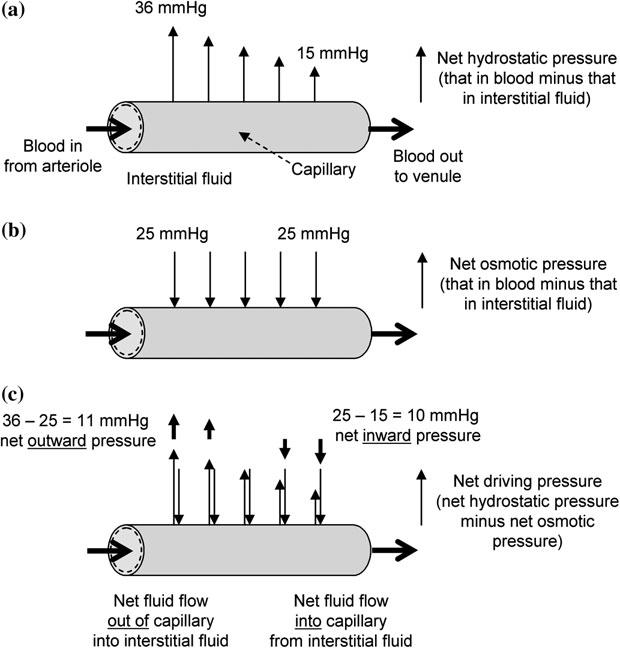
\includegraphics[width=0.55\textwidth]{823.png}
  \caption{Presión osmótica en un capilar (Basado en [66]).}
  \label{fig:823}
\end{figure}



una densidad mucho mayor de proteínas en la sangre que en el líquido intersticial, existe una fuerza impulsora química de fluido hacia el capilar para intentar igualar estas densidades. Esto conduce a una presión osmótica neta de aproximadamente $25\text{ mmHg}$ hacia el interior del capilar. En la Fig.~8.23, la presión neta es de $36\text{ mmHg} - 25\text{ mmHg} = 11\text{ mmHg}$ hacia afuera en el extremo de la arteriola y de $15\text{ mmHg} - 25\text{ mmHg} = -10\text{ mmHg}$ hacia adentro en el extremo de la vénula. Por lo tanto, hay un flujo neto hacia afuera del capilar en el extremo de la arteriola y un flujo neto hacia adentro del capilar en el extremo de la vénula. Existe un pequeño desequilibrio en esto y un pequeño flujo neto volumétrico hacia afuera del capilar.

Hemos asumido que el flujo en todos los vasos sanguíneos, incluidos los capilares, es laminar. Esto no puede ser realmente cierto para los capilares debido a que muchos de ellos tienen un diámetro interno de $5\text{ o }6\text{ }\mu\text{m}$ y los glóbulos rojos tienen un diámetro de aproximadamente $7{,}5\text{ }\mu\text{m}$. Los glóbulos rojos se deforman para pasar a través del capilar y el flujo resultante se denomina flujo de bolo (bolus flow). Los glóbulos rojos forman tapones y el plasma sanguíneo queda atrapado en las regiones entre estos tapones y se mueve en líneas de corriente. En ninguna otra parte del cuerpo es más evidente la naturaleza de múltiples componentes de la sangre.

% Control de Calidad: 26 párrafos origen -> 26 párrafos salida (párrafos 67 a 92). Mapeo 1:1 verificado. Sin omisiones.

Una función principal de este flujo sanguíneo capilar es la transferencia de oxígeno a las células, dejando sangre empobrecida en oxígeno en las venas. Como en (6.18), la tasa de consumo corporal de $\text{O}_2$, $\mathrm{d}V_{\text{O}_2}/\mathrm{d}t$, es igual al producto del gasto cardíaco $Q_{\text{t}}$ (véase más adelante) y la diferencia en la presión parcial de oxígeno en las arterias y venas, $p_{\text{a}} - p_{\text{v}}$,
\begin{equation}
\frac{\mathrm{d}V_{\text{O}_2}}{\mathrm{d}t} = Q_{\text{t}} (p_{\text{a}} - p_{\text{v}}).
\label{eq:828}
\end{equation}

Si los pulmones están introduciendo aire lo suficientemente rápido, entonces $p_{\text{a}} - p_{\text{v}}$ es fijo, y durante el ejercicio aeróbico $\mathrm{d}V_{\text{O}_2}/\mathrm{d}t$ aumenta linealmente con $Q_{\text{t}}$. Para una persona con una condición física promedio, la tasa máxima de flujo sanguíneo es de ${\approx}19\text{ L/min}$, para una persona con muy buena condición física es de ${\approx}25\text{ L/min}$, y para un atleta de élite puede ser de $35\text{ L/min}$.

El oxígeno se combina con la hemoglobina en los glóbulos rojos en los pulmones, donde la presión parcial de oxígeno es alta, aproximadamente $100\text{ mmHg}$. Es transportado en las arterias hacia los tejidos donde se libera debido a que la presión parcial de oxígeno es baja, y luego es utilizado. La sangre en las venas queda entonces empobrecida en oxígeno. La Figura~8.24a muestra la curva de disociación de hemoglobina-oxígeno. Claramente, la hemoglobina está saturada a más del $90\%$ con $\text{O}_2$ para presiones parciales superiores a $60\text{ mmHg de O}_2$. Los niveles aumentados de $\text{CO}_2$, el aumento de la temperatura y la disminución del pH desplazan esta curva hacia la derecha (Fig.~8.24b), lo cual mejora el rendimiento del cuerpo. En la Fig.~8.24a se observa que la curva de disociación para el pulmón se encuentra a la izquierda de la de los tejidos debido a que el pH es más alto y el nivel de $\text{CO}_2$ es más bajo en el pulmón, lo que aumenta la unión del oxígeno en los pulmones en comparación con la de los tejidos. Durante el ejercicio, el pH del tejido muscular cae y la presión parcial local de $\text{CO}_2$ y la temperatura local aumentan. Todos estos cambios desplazan la curva hacia la derecha y esto conduce a una mayor liberación de oxígeno (Fig.~8.24b). Durante el ejercicio, $p_{\text{a}} - p_{\text{v}}$ aumenta desde el valor en reposo de aproximadamente $50\text{ mL de oxígeno por L de sangre}$ a $150\text{ mL/L}$ en personas normales a $(\mathrm{d}V_{\text{O}_2}/\mathrm{d}t)_{\text{max}}$ (y a $160\text{--}170\text{ mL/L}$ en personas con muy buena condición física), en parte debido a que el flujo sanguíneo se desvía de los órganos hacia los músculos, donde la extracción de oxígeno es mayor debido al ejercicio (véase la Fig.~8.24).

\begin{figure}[htbp]
  \centering
  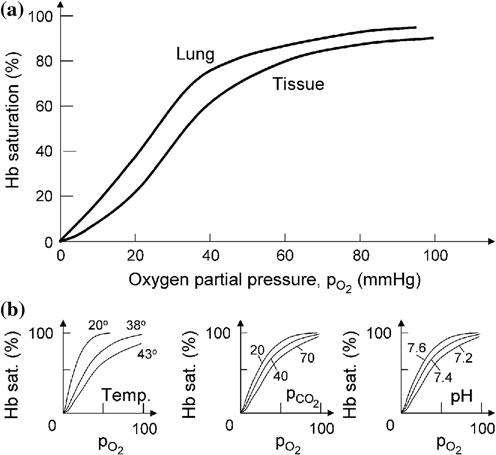
\includegraphics[width=0.55\textwidth]{824.png}
  \caption{a) Equilibrio de hemoglobina-oxígeno en los pulmones y tejidos. Durante el ejercicio, la captación de oxígeno mejora debido a que la curva pulmonar se desplaza hacia la izquierda y la curva tisular (músculo en ejercicio) se desplaza hacia la derecha debido al aumento de la temperatura, la presión parcial de $\text{CO}_2$ y el $2{,}3$-difosfoglicerato (DFG) (un producto final del metabolismo de los glóbulos rojos), y a la disminución del pH. b) El equilibrio de hemoglobina-oxígeno se desplaza hacia la derecha con el aumento de la temperatura, el aumento de la presión parcial de $\text{CO}_2$ y el aumento de DFG (no mostrado), y la disminución del pH (Basado en [60, 69]).}
  \label{fig:824}
\end{figure}



\subsection{Caudales y velocidades del flujo sanguíneo}

El corazón bombea aproximadamente $80\text{ mL}$ ($= 80\text{ cm}^3$) de sangre por contracción; esta cantidad se denomina volumen sistólico $V_{\text{stroke}}$. La frecuencia de bombeo es la frecuencia de latidos cardíacos $F$ de aproximadamente $60\text{ /min}$ o $1\text{ /s} = 1\text{ Hz}$. El gasto cardíaco o caudal volumétrico total $Q_{\text{t}}$ es el producto de estos dos
\begin{equation}
Q_{\text{t}} = F V_{\text{stroke}}
\label{eq:829}
\end{equation}
o aproximadamente $80\text{ cm}^3\text{/s} = 4{,}8\text{ L/min}$. El volumen total de sangre es de aproximadamente $4{,}5\text{--}5{,}0\text{ L}$, por lo que toda la sangre se bombea por todo el cuerpo cada minuto. Los caudales en las arterias, arteriolas, capilares, vénulas y venas son todos los mismos debido a la continuidad del flujo. (En realidad, $Q_{\text{t}}$ es un poco menor en las vénulas y venas debido a la pérdida neta de líquido en los capilares). Durante el término completo del embarazo, el gasto cardíaco aumenta en un ${\sim}30\%$, de ${\sim}5{,}0$ a $6{,}7\text{ L/min}$ debido al aumento del volumen sistólico y de la frecuencia cardíaca, y el volumen sanguíneo aumenta en un ${\sim}40\text{--}50\%$ [47, 55].

El flujo total en cada uno de estos sistemas de vasos, $Q_{\text{t}}$, es igual al área de sección transversal total $A$ multiplicada por la velocidad de la sangre $u$, $Q_{\text{t}} = A u$. Los parámetros $A$ y $u$ se representan en la Fig.~8.16, la cual muestra esta relación inversa para un caudal de $90\text{ cm}^3\text{/s}$. El área de sección transversal de la aorta es de $3\text{ cm}^2$, por lo que en la aorta $u = (90\text{ cm}^3\text{/s})/3\text{ cm}^2 = 30\text{ cm/s}$. En los capilares, la velocidad de flujo es mucho más lenta, $(90\text{ cm}^3\text{/s})/4\,000\text{ cm}^2 = 0{,}022\text{ cm/s} = 0{,}22\text{ mm/s}$. El área de sección transversal neta en los capilares es mayor (${\sim}4\,000\text{ cm}^2$), a pesar de que son muy pequeños (${\sim}3{,}5\text{ }\mu\text{m}$ de radio), debido a que hay muchísimos de ellos (${\sim}10^{10}$). En la vena cava, la velocidad de flujo es relativamente rápida, $(90\text{ cm}^3\text{/s})/18\text{ cm}^2 = 5\text{ cm/s}$. En los sistemas arterial y venoso, cuanto menor es el radio del vaso, mayor es la sección transversal total de todos los vasos en ese orden y más lenta es la velocidad de la sangre. Estos son en realidad flujos sanguíneos promedio durante cada ciclo.

El número de Reynolds máximo ($R_{\text{e}} = \rho u d/\eta$, (7.11)) a lo largo de un ciclo cardíaco varía desde ${\sim}6\,000$ en el corazón y la aorta hasta $<10^{-3}$ en los capilares. El umbral inferior nominal para el flujo turbulento es $R_{\text{e}} \sim 2\,000$, por lo que es posible que el flujo en la aorta sea turbulento.

El flujo general en el sistema arterial sistémico se puede describir relacionando el gasto cardíaco total $Q_{\text{t}}$ con la presión arterial sistémica $P_{\text{sa}}$ mediante
\begin{equation}
P_{\text{sa}} = (\text{TPVR}) Q_{\text{t}},
\label{eq:830}
\end{equation}
donde TPVR es la resistencia vascular periférica total (total peripheral vascular resistance), la cual se debe al efecto combinado de todos los lechos orgánicos de la circulación sistémica (principalmente arteriolas y capilares). (En realidad, $P_{\text{sa}}$ debería reemplazarse por la caída de presión en el sistema. Véase el Problema 8.21). Los valores normales para el sistema sistémico varían de $700$ a $1\,600\text{ dina}\cdot\text{s/cm}^5$, y los valores normales análogos para el sistema pulmonar varían de $20$ a $130\text{ dina}\cdot\text{s/cm}^5$. La ecuación (8.2) se aplica a un vaso individual, mientras que esta relación describe a todo el sistema sistémico. El cuerpo regula $P_{\text{sa}}$ controlando el gasto cardíaco y esta resistencia periférica. Cuando nos acostamos, un gran volumen de sangre se almacena transitoriamente en las extremidades inferiores y el abdomen, por lo que cuando nos ponemos de pie hay inicialmente menos flujo de sangre al corazón y una caída en la presión arterial, lo cual puede hacer que uno se desmaye. Aunque $Q_{\text{t}}$ disminuye, $P_{\text{sa}}$ cae solo levemente debido a que existe un reflejo rápido que aumenta la TPVR (vasoconstricción). En contraste, cuando la presión arterial aumenta repentinamente, la retroalimentación tiende a disminuir la resistencia vascular general para restablecer una presión arterial más baja. Estos son dos ejemplos de retroalimentación y control del cuerpo, como se describe en el Cap.~13.

También evaluamos las compliancias generales de los sistemas vasculares, tales como las de los sistemas arterial y venoso sistémicos. La compliancia es el recíproco de la pendiente de una curva de presión-volumen en la Fig.~8.25. Los músculos lisos que rodean un vaso grande pueden cambiar el volumen del vaso a una presión dada, ya sea disminuyéndolo (estimulando los músculos) o aumentándolo (inhibiendo los músculos).

\begin{figure}[htbp]
  \centering
  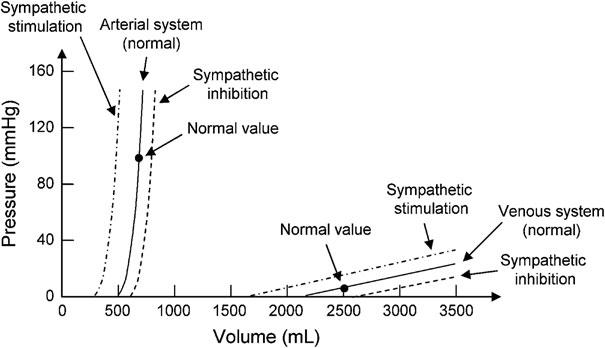
\includegraphics[width=0.8\textwidth]{825.png}
  \caption{Curvas de volumen-presión para los sistemas arterial y venoso sistémicos, para condiciones normales y para la estimulación e inhibición simpática (Basado en [29]).}
  \label{fig:825}
\end{figure}



Durante el ejercicio, incluso moderado, el caudal sanguíneo aumenta sustancialmente, como se ve en la Fig.~8.26, y la distribución absoluta y relativa de la sangre a diferentes partes del cuerpo también cambia radicalmente. La Figura~8.27 muestra un ejemplo en el que el caudal aumenta de $5$ a $12{,}5\text{ L/min}$ durante el ejercicio. Ocurren aumentos extremadamente grandes de sangre que fluye hacia el músculo esquelético para suministrar oxígeno para el metabolismo aeróbico (hasta un $1\,066\%$), hacia el corazón para que pueda bombear más rápido (hasta un $367\%$) y hacia la piel (hasta un $370\%$) para ayudar al enfriamiento (lo cual aumenta la temperatura de la piel, acelerando así la conducción por radiación y convección desde el cuerpo). El flujo de sangre al cerebro no cambia. En contraste, el flujo de sangre al tracto digestivo, al hígado y a los riñones disminuye en un factor de ${\sim}2$. Estos cambios también se observan en las Tablas~8.6 y 8.7. La Figura~8.28 muestra que el flujo sanguíneo a la pantorrilla durante el ejercicio rítmico es mayor de lo normal y varía con el tiempo.

\begin{SCfigure}[0.8][htbp]
  \centering
  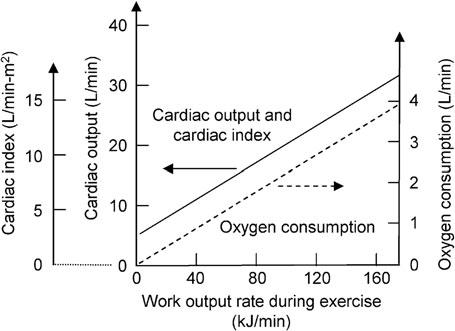
\includegraphics[width=0.55\textwidth]{826.png}
  \caption{Variación en el gasto cardíaco (y el índice cardíaco) y el consumo de oxígeno necesarios durante diferentes niveles de ejercicio con la potencia de trabajo (El índice cardíaco es el gasto cardíaco dividido por el área superficial de la persona) (Basado en [28, 29]).}
  \label{fig:826}
\end{SCfigure}

\begin{figure}[htbp]
  \centering
  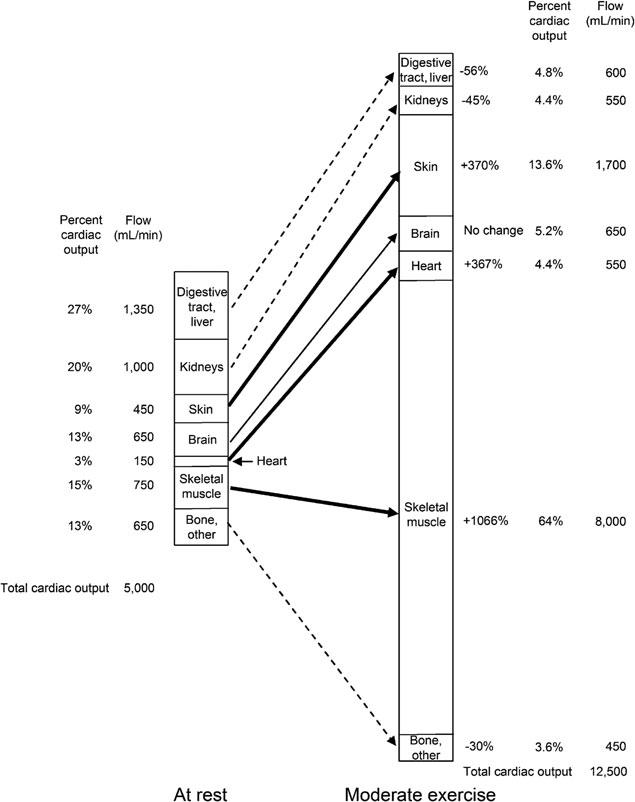
\includegraphics[width=0.45\textwidth]{827.png}
  \caption{Flujo sanguíneo a diferentes órganos en reposo y durante el ejercicio moderado, mostrando que no hay cambios en el cerebro, aumentos en la piel, el corazón y los músculos esqueléticos (flechas gruesas), y menor flujo sanguíneo en otros lugares (flechas discontinuas) (Basado en [66]).}
  \label{fig:827}
\end{figure}

\begin{figure}[htbp]
  \centering
  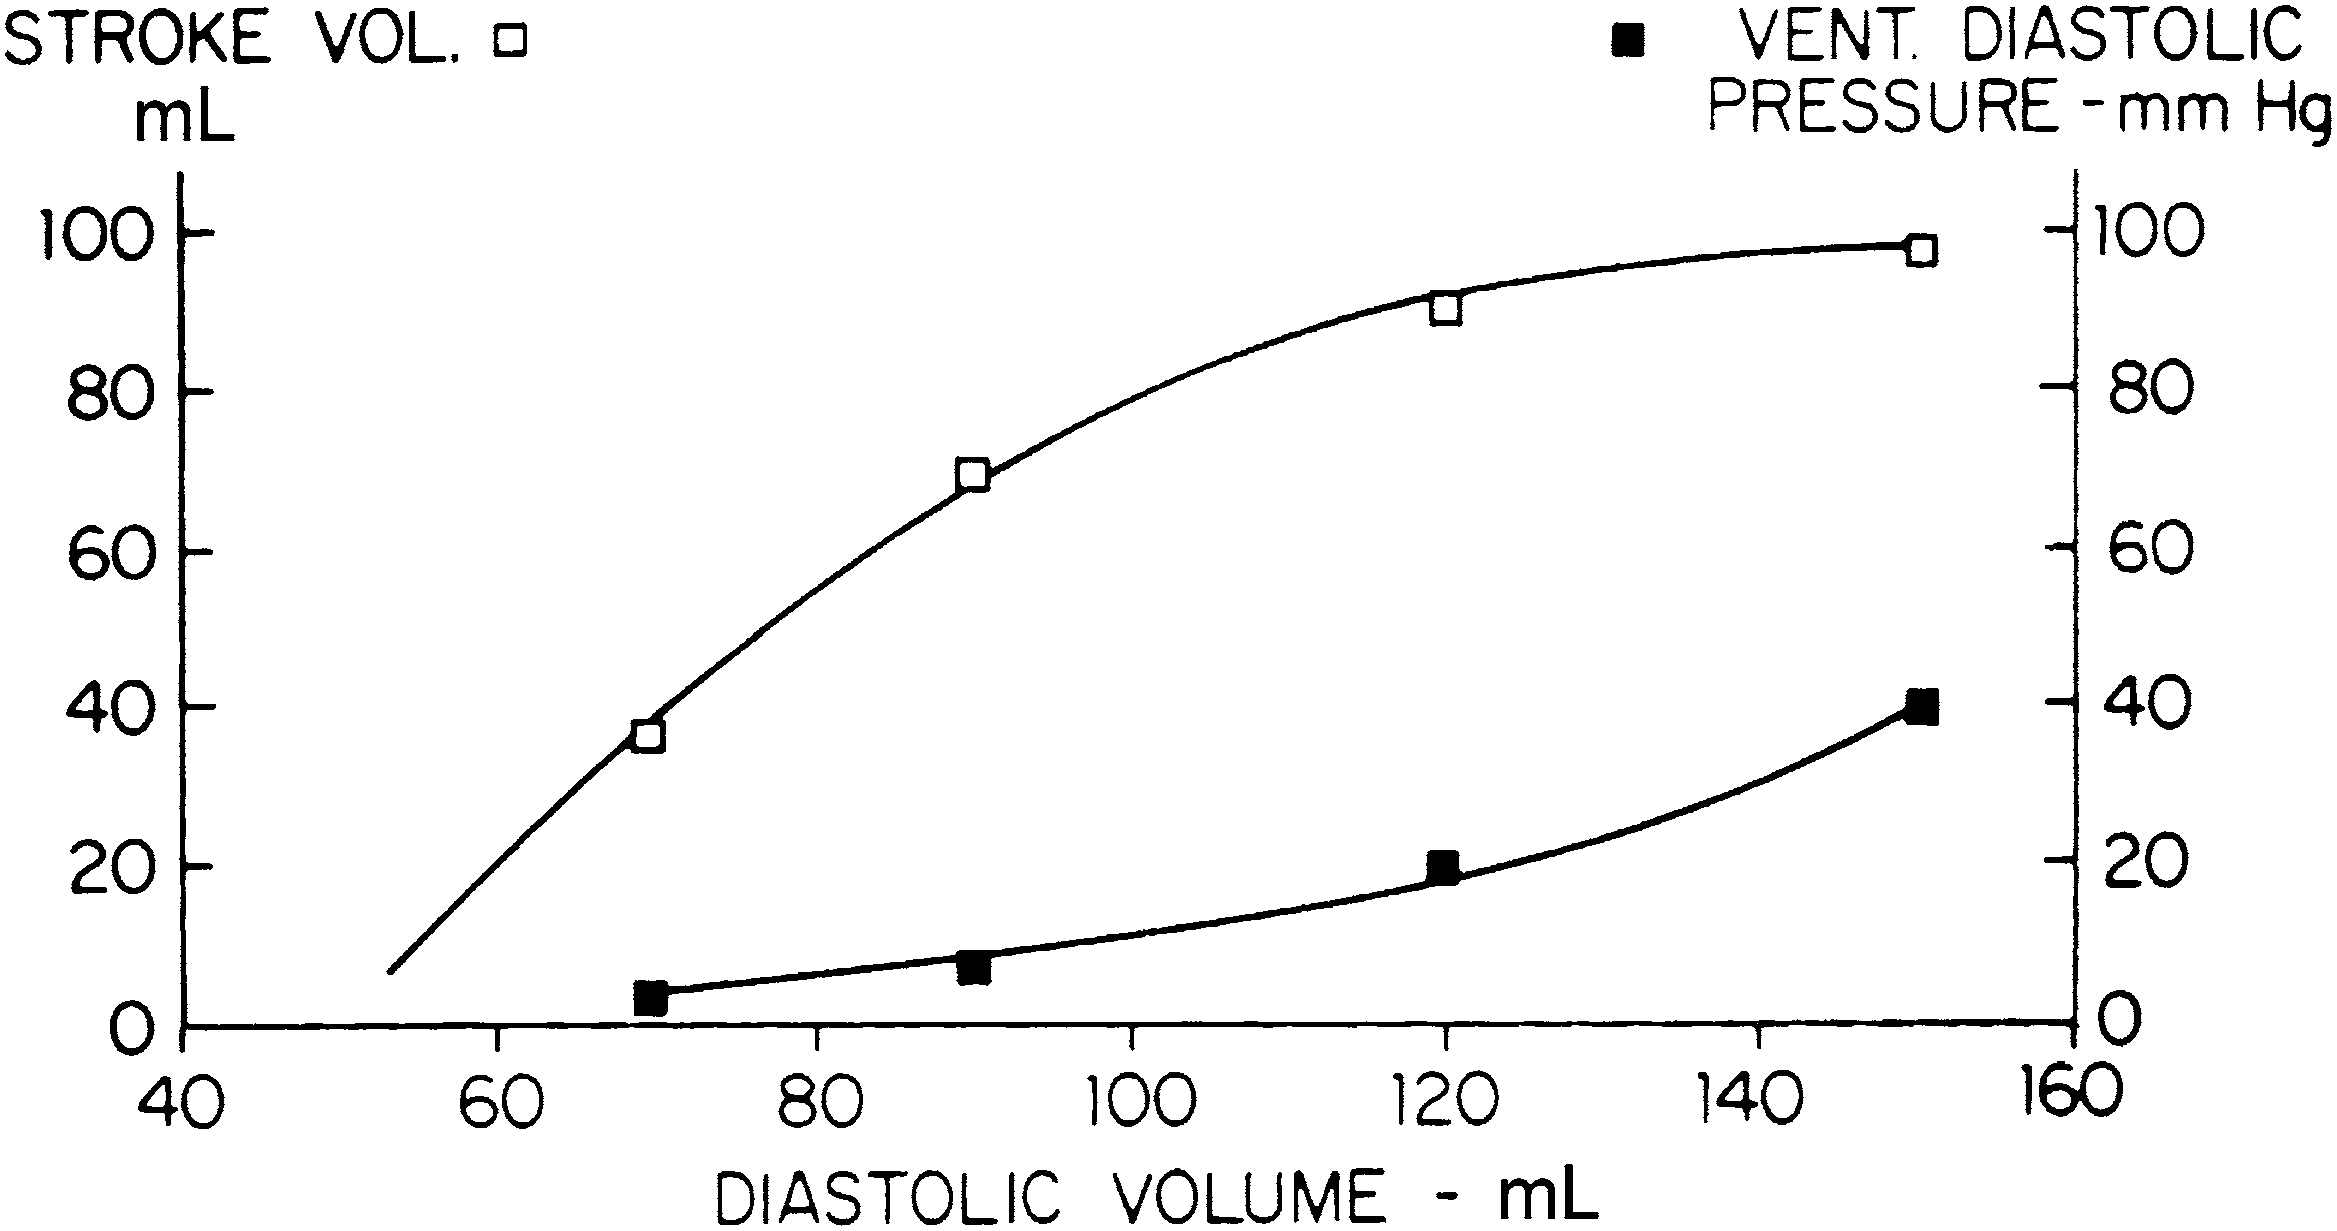
\includegraphics[width=0.8\textwidth]{828.png}
  \caption{Flujo sanguíneo a la pantorrilla durante ejercicios de contracción rítmica, mostrando menor flujo sanguíneo durante las contracciones que entre ellas (Basado en [3, 29]).}
  \label{fig:828}
\end{figure}



Este aumento en el gasto cardíaco durante el ejercicio ocurre debido a incrementos tanto en la frecuencia cardíaca como en el volumen sistólico; la velocidad de la sangre también aumenta porque $Q_{\text{t}} = A u$. Cuanto más rápida es la frecuencia cardíaca, más corta es la diástole, mientras que la duración de la sístole no cambia. Para el ejercicio submáximo a corto plazo ($5\text{--}10\text{ min}$), el gasto cardíaco aumenta de $5\text{ L/min}$ a un nuevo valor de estado estacionario en aproximadamente $2\text{ min}$. Para un gasto cardíaco en estado estacionario de $18\text{ L/min}$, el volumen sistólico aumenta de aproximadamente $70\text{--}120\text{ mL/latido}$ y la frecuencia cardíaca $F$ de aproximadamente $70\text{--}150\text{ latidos/min}$. El gasto cardíaco regresa al valor de reposo en $5\text{--}10\text{ min}$ después del ejercicio.

Para un entrenamiento submáximo más prolongado ($30\text{--}60\text{ min}$), se mantiene el nuevo gasto cardíaco en estado estacionario, pero el volumen sistólico disminuye lentamente y la frecuencia cardíaca aumenta gradualmente con el tiempo, particularmente en ambientes más cálidos. Esta deriva cardiovascular (cardiovascular drift) es causada por una disminución en el retorno venoso de sangre al corazón, lo cual disminuye el volumen sistólico y, por lo tanto, la frecuencia cardíaca debe aumentar para mantener el mismo gasto cardíaco. Esta disminución en el retorno venoso es causada por dos factores. (1) Durante dicho ejercicio, fluye más sangre debajo de la piel para ayudar a reducir el aumento de la temperatura corporal central causado por el incremento de la actividad metabólica (Cap.~6), y esto reduce el flujo de sangre de retorno en estado estacionario. (2) Durante el ejercicio, el agua fluye desde la sangre hacia las células y tejidos circundantes debido al aumento de la presión arterial y la compresión de las vénulas debido a la acción muscular. Esto produce una disminución en estado estacionario del plasma sanguíneo y del volumen de sangre, y una disminución en estado estacionario de la sangre que regresa al corazón y del volumen sistólico.

El volumen sistólico y el gasto cardíaco están determinados por las condiciones de precarga y poscarga (véase más adelante), la contractilidad (capacidad de contraerse) y la frecuencia cardíaca. El gasto cardíaco no está regulado directamente, pero existe un sistema de retroalimentación y control que regula la presión arterial el cual afecta la frecuencia cardíaca y la contractilidad, así como la poscarga y otros factores que controlan la precarga [64].

El mecanismo de Frank-Starling (o ley de Starling del corazón) establece que cuanto mayor sea el volumen o la presión al final de la diástole (la precarga), mayor será el volumen sistólico, como se observa en la Fig.~8.29. Además, cuanto mayor sea la presión aórtica, menos sangre puede ser expulsada por el ventrículo izquierdo (la poscarga), como se observa en la Fig.~8.30. Un aumento en la frecuencia cardíaca también incrementa el gasto cardíaco; sin embargo, el incremento es sublineal debido a que el volumen sistólico disminuye (Fig.~8.31) por los factores de precarga y poscarga antes mencionados. Con un mayor gasto cardíaco, hay menos sangre en las venas para retornar al corazón durante la diástole (menor precarga) y la presión arterial es mayor, por lo que el corazón puede expulsar menos sangre (mayor poscarga), asumiendo que la resistencia periférica es constante.

\begin{figure}[htbp]
  \centering
  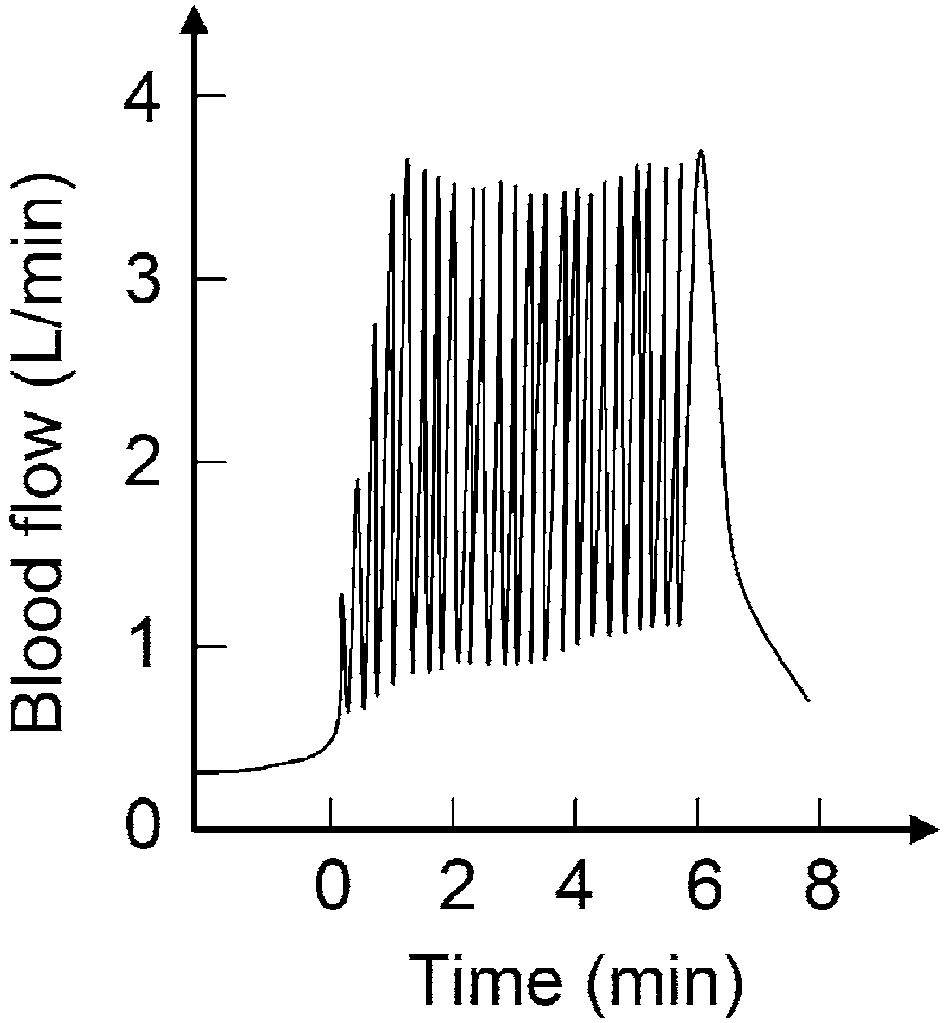
\includegraphics[width=0.55\textwidth]{829.png}
  \caption{El volumen sistólico aumenta con el volumen y la presión diastólica, como se observa con datos de cuatro latidos cardíacos. Esta dependencia, junto con su explicación, se conoce como el mecanismo de Frank-Starling (Reimpreso de [64]. Con autorización de Elsevier).}
  \label{fig:829}
\end{figure}

\begin{SCfigure}[0.8][htbp]
  \centering
  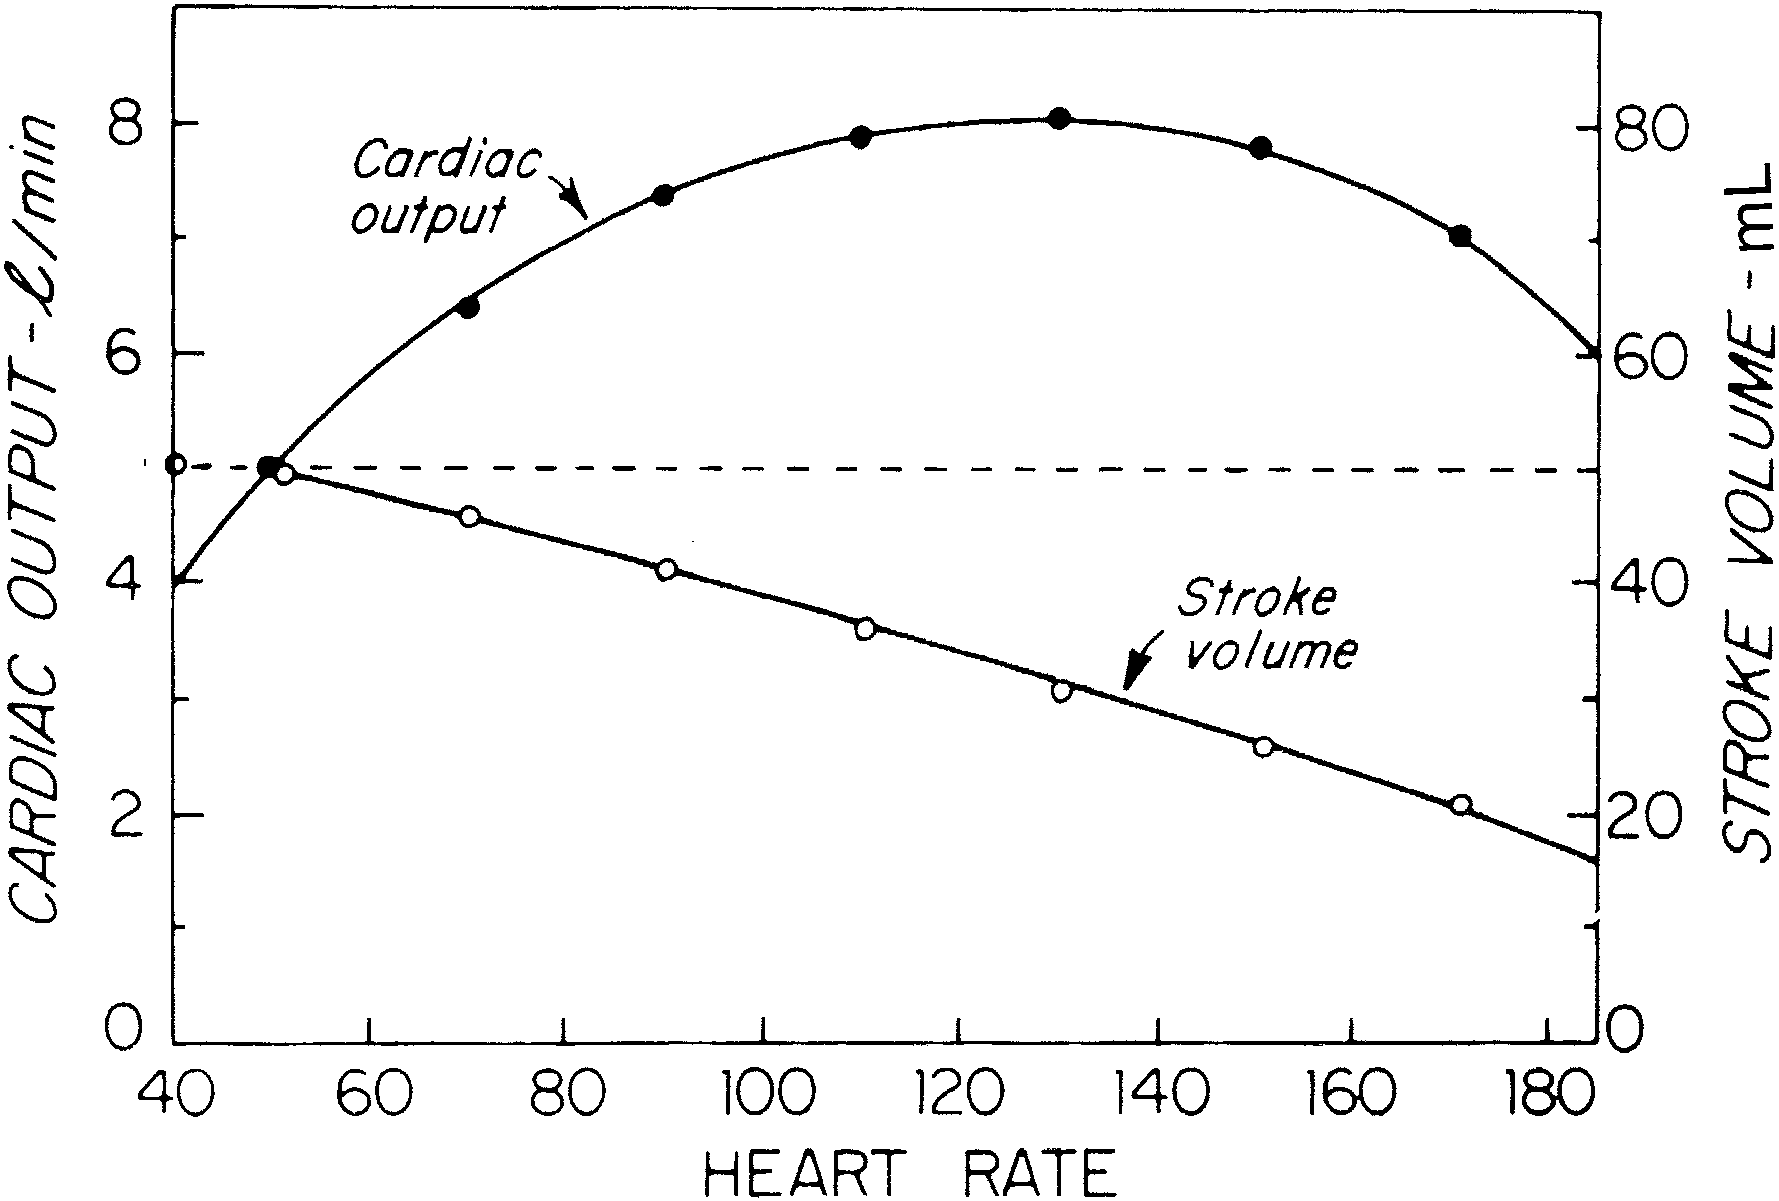
\includegraphics[width=0.55\textwidth]{830.png}
  \caption{El gasto del ventrículo izquierdo (el gasto cardíaco) frente a la presión auricular izquierda para diferentes presiones aórticas. Aumenta con esta presión auricular y luego se estabiliza, y disminuye al aumentar la presión aórtica (Reimpreso de [64]. Con autorización de Elsevier; adaptado de [62]).}
  \label{fig:830}
\end{SCfigure}

\begin{SCfigure}[1.0][htbp]
  \centering
  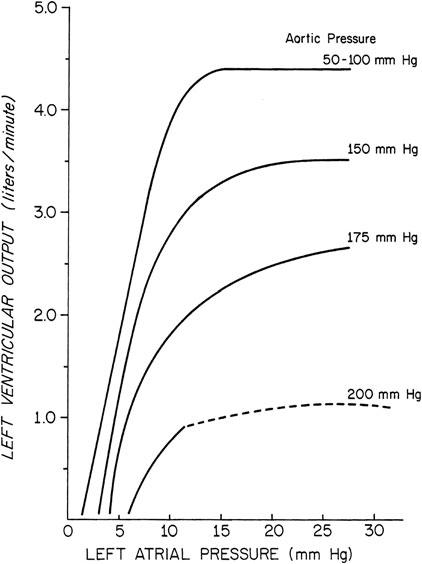
\includegraphics[width=0.45\textwidth]{831.png}
  \caption{Dependencia típica del gasto cardíaco y del volumen sistólico con la frecuencia cardíaca (Reimpreso de [64]. Con autorización de Elsevier).}
  \label{fig:831}
\end{SCfigure}



\begin{table}[htbp]
\centering
\caption{Flujo cardíaco total ($\text{mL/min}$) para órganos durante el ejercicio, incluyendo el porcentaje del flujo total}
\label{tab:86}
\small
\begin{tabularx}{\textwidth}{X *{4}{>{\centering\arraybackslash}p{2.6cm}}}
\toprule
\textbf{Órgano} & \textbf{Reposo} & \textbf{Ejercicio ligero} & \textbf{Ejercicio intenso} & \textbf{Ejercicio máximo} \\
\midrule
Cerebro & $750$ ($13\%$) & $750$ ($8\%$) & $750$ ($4\%$) & $750$ ($3\%$) \\
Corazón & $250$ ($4\%$) & $350$ ($3{,}5\%$) & $750$ ($4\%$) & $1\,000$ ($4\%$) \\
Músculo & $1\,200$ ($21\%$) & $4\,500$ ($47\%$) & $12\,500$ ($72\%$) & $22\,000$ ($88\%$) \\
Piel & $500$ ($8{,}5\%$) & $1\,500$ ($16\%$) & $1\,900$ ($11\%$) & $600$ ($2{,}5\%$) \\
Riñón & $1\,100$ ($19\%$) & $900$ ($9{,}5\%$) & $600$ ($3{,}5\%$) & $250$ ($1\%$) \\
Abdomen & $1\,400$ ($24\%$) & $1\,100$ ($11{,}5\%$) & $600$ ($3{,}5\%$) & $300$ ($1{,}2\%$) \\
Otros & $600$ ($10{,}5\%$) & $400$ ($4\%$) & $400$ ($2\%$) & $100$ ($0{,}4\%$) \\
\midrule
Total & $5\,800$ ($100\%$) & $9\,500$ ($100\%$) & $17\,500$ ($100\%$) & $25\,000$ ($100\%$) \\
\bottomrule
\end{tabularx}
\begin{flushleft}
    \small Usando datos de [20].
\end{flushleft}
\end{table}

\begin{table}[htbp]
\centering
\caption{Flujo sanguíneo aproximado (perfusión) para tejidos y órganos, por gramo}
\label{tab:87}
\small
\begin{tabularx}{\textwidth}{l X c}
\toprule
\textbf{Tipo de tejido} & \textbf{Ubicación u órgano} & \textbf{Tasa de flujo sanguíneo específica ($\text{mm}^3\text{/s}\cdot\text{g}$)} \\
\midrule
Tejido adiposo & Abdomen, ${\sim}20\text{ mm}$ de espesor & $0{,}51$ \\
 & Abdomen, $>40\text{ mm}$ de espesor & $0{,}31$ \\
 & Muslo, ${\sim}20\text{ mm}$ de espesor & $0{,}33$ \\
Hueso & Húmero, solo flujo de médula & $0{,}055$ \\
Tejido conectivo & Basal típico (máx.) & $0{,}50$ ($2{,}5$) \\
Músculo & Basal típico (máx.) & $0{,}50$ ($10$) \\
Órgano & Cerebro, basal (máx.) & $9{,}1$ ($18{,}3$) \\
 & Tracto gastrointestinal, basal (máx.) & $6{,}7$ ($26{,}7$) \\
 & Corazón, basal (máx.) & $13{,}7$ ($64{,}0$) \\
 & Riñón, basal (máx.) & $68$ ($100$) \\
 & Hígado, basal (máx.) & $12$ ($54$) \\
 & Pulmón, basal (máx.) & $90$ ($490$) \\
Piel & Flujo típico en reposo (máx.) & $1{,}7$ ($25{,}0$) \\
\bottomrule
\end{tabularx}
\begin{flushleft}
    \small Usando datos de [21].\\
    En algunos casos se proporciona la tasa basal, junto con la tasa máxima entre paréntesis.
\end{flushleft}
\end{table}

En su mayor parte, estos son cambios en el sistema sistémico. Incrementos similares en el gasto cardíaco deben ocurrir en el sistema pulmonar. (¿Por qué?) Esto ocurre por un aumento en el número de capilares abiertos en el pulmón, hasta en un factor de tres, y por una distensión de todos los capilares pulmonares, lo que incrementa el flujo en cada capilar hasta en un factor de dos, con muy pocos cambios en la presión arterial pulmonar (Fig.~8.32).

\begin{SCfigure}[0.8][htbp]
  \centering
  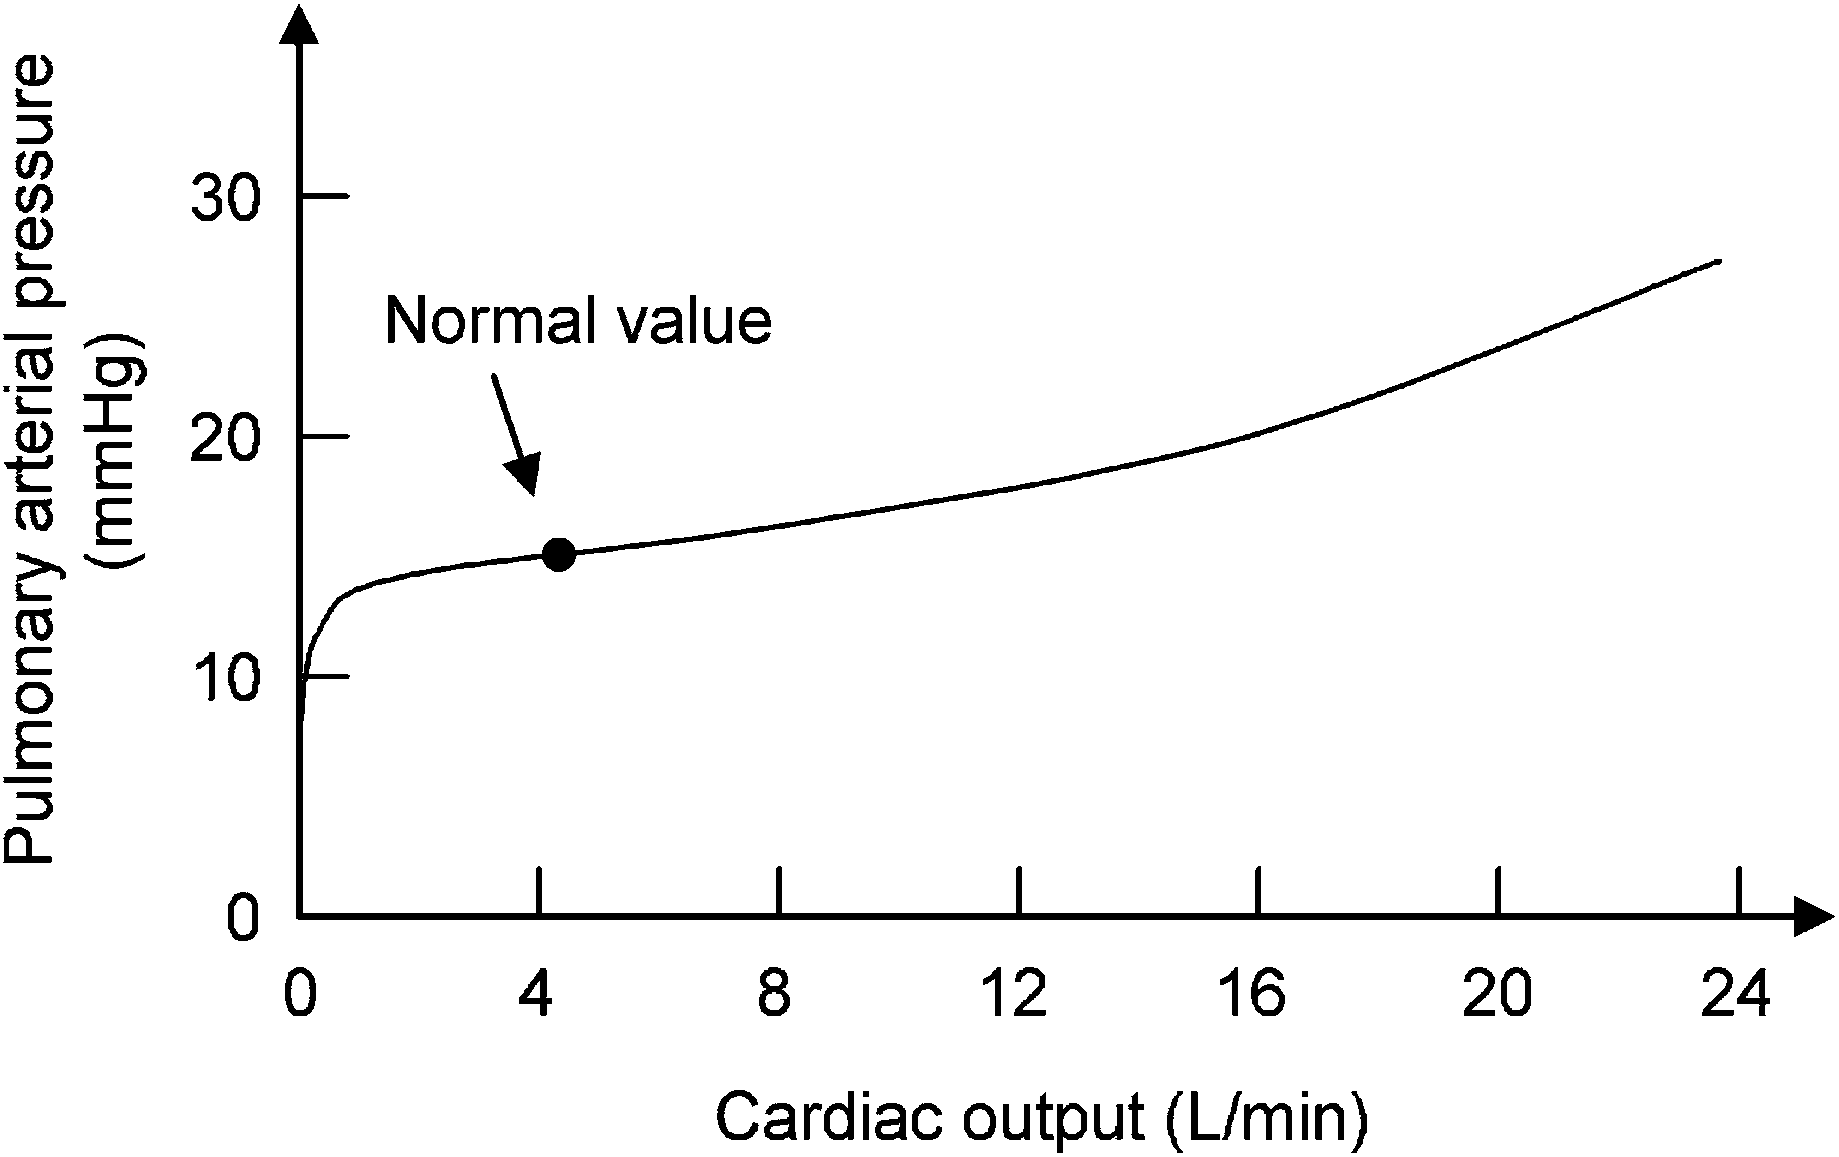
\includegraphics[width=0.55\textwidth]{832.png}
  \caption{La presión arterial pulmonar frente a la presión cardíaca, mostrando que no cambia mucho durante el ejercicio (Basado en [29]).}
  \label{fig:832}
\end{SCfigure}



La frecuencia cardíaca máxima $F_{\text{max}}$ (en latidos/min) depende de la edad $Y$ (en años). Usualmente se expresa como
\begin{equation}
F_{\text{max}} = 220 - Y,
\label{eq:831}
\end{equation}
pero trabajos recientes [56] sugieren que
\begin{equation}
F_{\text{max}} = 211 - 0{,}64 Y
\label{eq:832}
\end{equation}
es más preciso. El error estándar en estas relaciones es de $\pm 10\text{ latidos/min}$, lo que significa que el $67\%$ de las personas tienen una frecuencia máxima de $\pm 10\text{ latidos/min}$ del valor predicho por estas relaciones y el $95\%$ de todas las personas tienen una frecuencia que está a $\pm 20\text{ latidos/min}$ de los valores predichos.

Debido a que $F$ no depende del nivel de condición física, los atletas aumentan su gasto cardíaco máximo incrementando sus volúmenes sistólicos. Los volúmenes sistólicos en atletas no entrenados son de $50\text{--}70\text{ mL}$ en reposo y alcanzan $80\text{--}110\text{ mL}$ durante la actividad intensa. Para atletas entrenados y altamente entrenados, estos volúmenes sistólicos aumentan a $70\text{--}90\text{ mL}$ y $90\text{--}110\text{ mL}$ en reposo y a $110\text{--}150\text{ mL}$ y $150\text{--}220\text{ mL}$ durante la actividad intensa.

En estado estacionario, el gasto cardíaco $Q_{\text{t}}$ debe ser igual a $F V_{\text{stroke}}$ (8.29), así como a $P_{\text{sa}}/\text{TPVR}$ (8.30). Durante el ejercicio intenso, $Q_{\text{t}}$ aumenta de $5$ a $20\text{ L/min}$, por lo que no solo deben aumentar $F$ y $V_{\text{stroke}}$, como hemos descrito, sino que $P_{\text{sa}}/\text{TPVR}$ debe aumentar en consecuencia. La presión diastólica cambia poco durante el ejercicio, permaneciendo dentro de $\pm 10\text{ mmHg}$ del valor en reposo. La presión sistólica aumenta a aproximadamente $200\text{ mmHg}$ para los hombres y $180\text{ mmHg}$ para las mujeres. Usando (8.1), la presión arterial media entonces aumenta solo a $140\text{--}150\text{ mmHg}$, lo cual no puede explicar la mayor parte del incremento en la tasa de flujo sanguíneo. Durante el ejercicio intenso, la resistencia vascular sistémica TPVR disminuye a aproximadamente el $40\%$ de su valor en reposo debido al ensanchamiento de los lechos vasculares musculares que normalmente están constreñidos a niveles bajos de actividad.

Con la edad avanzada, el gasto cardíaco y la fracción de eyección no cambian para una persona sana, pero el gasto cardíaco máximo disminuye con la edad. En el ejercicio máximo en hombres entrenados en resistencia, este disminuye en un ${\sim}20\%$ desde ${\sim}27{,}0\text{ L/min}$ a los $28\text{ años}$ de edad a ${\sim}21{,}7\text{ L/min}$ a los $60\text{ años}$ debido a disminuciones del ${\sim}10\%$ en el volumen sistólico, de ${\sim}147$ a ${\sim}132\text{ mL}$, y en la frecuencia cardíaca, de ${\sim}184\text{ latidos/min}$ a ${\sim}165\text{ latidos/min}$ [1, 19, 67]. (Como se ve más adelante, la fracción de eyección es el volumen sistólico dividido por el volumen ventricular al final de la diástole, el cual es normalmente del $55\text{--}75\%$).

La Figura~8.33 muestra que la presión arterial típicamente aumenta con la edad. La hipertensión comienza con una presión sistólica $\ge 140\text{ mmHg}$ o una presión diastólica $\ge 90\text{ mmHg}$. En la hipertensión esencial, esta presión arterial se eleva sin ninguna razón obvia. La presión arterial promedio es el producto de la resistencia vascular periférica total y el gasto cardíaco, $P_{\text{sa}} = (\text{TPVR}) Q_{\text{t}}$ (8.30). En personas menores de $40\text{ años}$, la hipertensión es impulsada por un aumento en el gasto cardíaco, con una TPVR normal. En personas mayores, el gasto cardíaco es normal o reducido, pero la TPVR es alta.

\begin{SCfigure}[0.8][htbp]
  \centering
  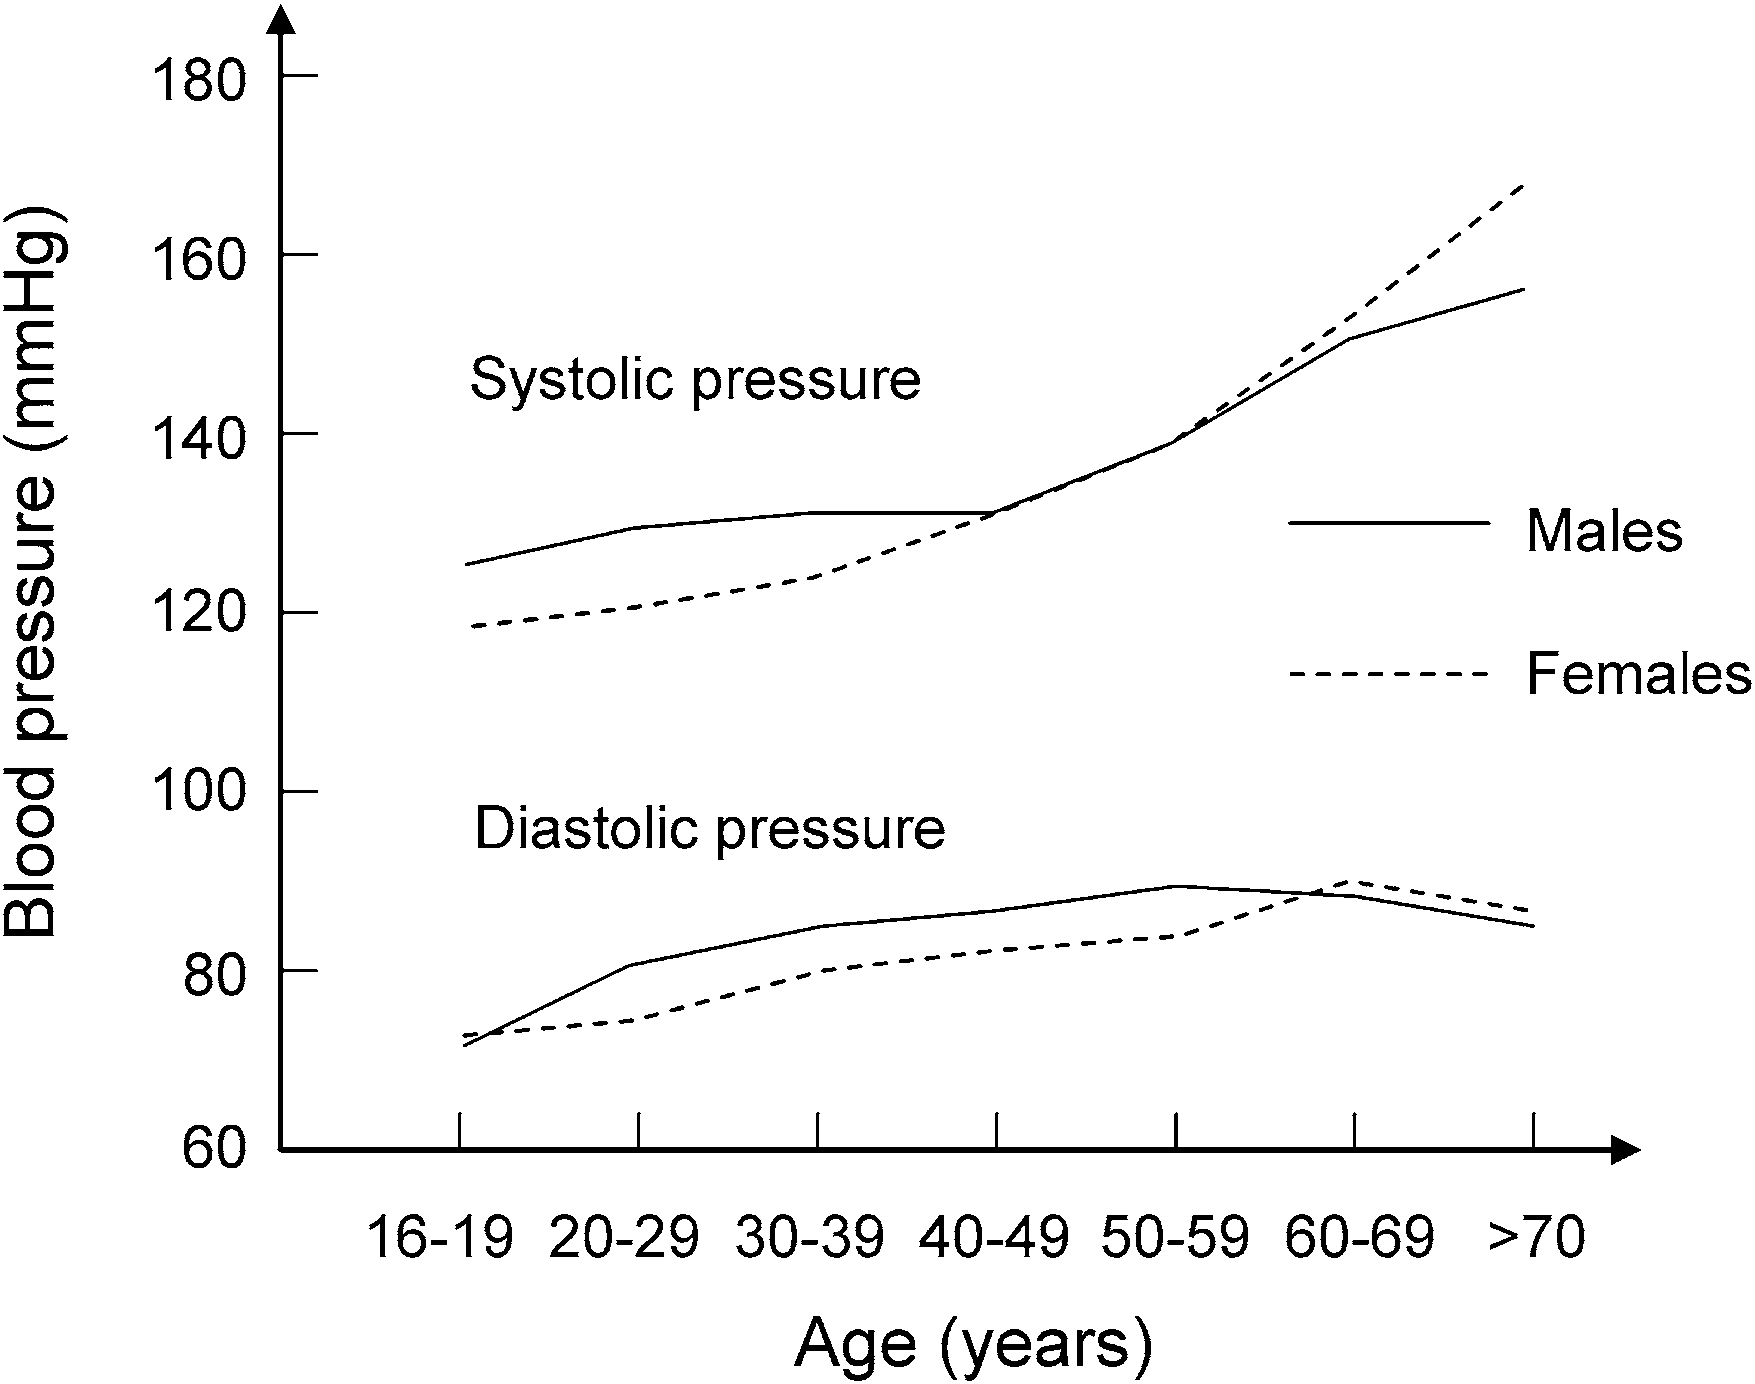
\includegraphics[width=0.55\textwidth]{833.png}
  \caption{Se muestra la presión arterial sistólica y diastólica para hombres y mujeres, promediada por grupos de edad. La tendencia es al aumento de la presión arterial con la edad (Basado en [43, 48]).}
  \label{fig:833}
\end{SCfigure}



En el feto, el gasto cardíaco combinado es la suma del gasto cardíaco de los ventrículos derecho e izquierdo; aumenta desde ${\sim}210\text{ mL/min}$ a las $20\text{ semanas}$ a ${\sim}1\,900\text{ mL/min}$ a las $38\text{ semanas}$, y se distribuye de manera muy aproximada por igual entre los ventrículos [41]. (Después del nacimiento, el gasto cardíaco se define claramente como la cantidad total de cualquiera de los dos ventrículos). Cerca del final de la gestación, un ${\sim}20\%$ y un ${\sim}40\%$ de este total se desvía a través del foramen oval y el conducto arterioso. El flujo sanguíneo a través del cordón umbilical es de ${\sim}35\text{ mL/min}$ a las $20\text{ semanas}$ y de ${\sim}240\text{ mL/min}$ a las $40\text{ semanas}$ de gestación, una fracción pequeña pero significativa del gasto cardíaco combinado. La fracción de sangre que regresa del cordón umbilical desviada hacia el conducto venoso disminuye desde un ${\sim}30\%$ a la mitad de la gestación a un ${\sim}20\%$ cerca del final de la misma, y el resto va al hígado. El peso de la sangre en el feto es del ${\sim}10\text{--}12\%$ del peso corporal (incluyendo la placenta, con un ${\sim}33\%$ en la placenta al nacer), lo cual es un poco mayor que el ${\sim}7\text{--}8\%$ en los adultos; excluyendo la placenta, esto corresponde a aproximadamente $80\text{ mL de sangre por kg de masa fetal}$. La presión sistólica sistémica en el feto aumenta a ${\sim}30\text{--}40\text{ mmHg}$ a las $28\text{ semanas}$ de gestación.

El choque circulatorio en las personas ocurre cuando hay muy poco flujo sanguíneo general en el cuerpo, lo que resulta en daño tisular debido al suministro inadecuado de oxígeno y nutrientes a las células y a la eliminación inadecuada de productos de desecho. Dicho choque puede ocurrir por un bombeo inadecuado de sangre por parte del corazón o por un retorno venoso inadecuado de sangre al corazón, debido, por ejemplo, a una disminución del volumen sanguíneo (hipovolemia), una disminución de la vasomotilidad capilar o una circulación obstrucida. La hemorragia suele ser la causa de la disminución del volumen sanguíneo. La Figura~8.34 muestra que el gasto cardíaco y la presión arterial pueden soportar una pérdida de sangre de ${\sim}10\%$ ---si esto no fuera así, no se podría donar sangre---, pero disminuyen ante pérdidas mayores y se aproximan a cero con una pérdida de sangre del $35\text{--}45\%$. La pérdida localizada de flujo sanguíneo al cerebro, los accidentes cerebrovasculares, se analiza más adelante. Esto ocurre debido a arterias obstruidas (como veremos de vez en cuando más adelante) y a hemorragias (como veremos más abajo). La pérdida localizada de flujo sanguíneo al corazón produce un infarto de miocardio (ataque al corazón).

\begin{SCfigure}[0.75][htbp]
  \centering
  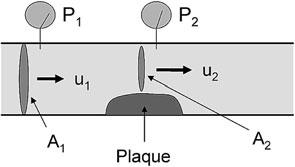
\includegraphics[width=0.6\textwidth]{834.png}
  \caption{Gasto cardíaco y presión arterial con volumen sanguíneo disminuido por hemorragia (Basado en [29]).}
  \label{fig:834}
\end{SCfigure}



\subsection{Consecuencias de las arterias obstruidas}

La aterosclerosis (a-te-ro-es-cle-ro-sis) ocurre cuando un depósito o ateroma (a-te-ro-ma) (o placa) se forma en una pared arterial (Fig.~8.35). La menor área de sección transversal en este sitio, dado que $A_2/A_1 < 1$, conduce a una mayor velocidad de flujo debido a la continuidad del flujo, con
\begin{equation}
u_2 = \frac{A_1}{A_2} u_1
\label{eq:833}
\end{equation}
a partir de (7.16). Para $A_2/A_1 = 1/3$, encontramos que $u_2 = 3u_1$. También a partir de la ecuación de Bernoulli (7.18) encontramos que
\begin{equation}
P_2 - P_1 = \frac{1}{2} \rho u_1^2 \left( 1 - \left( \frac{A_1}{A_2} \right)^2 \right)
\label{eq:834}
\end{equation}
y por lo tanto $P_2 < P_1$, y para $A_2/A_1 = 1/3$ vemos que $P_2 - P_1 = -4\rho u_1^2$. Esta caída de presión aumenta con la velocidad de la sangre, por lo que se espera que aumente con el incremento de la actividad física. Este flujo no es necesariamente laminar en la región ocluida, como se observa en la Fig.~8.36.

\begin{SCfigure}[0.8][htbp]
  \centering
  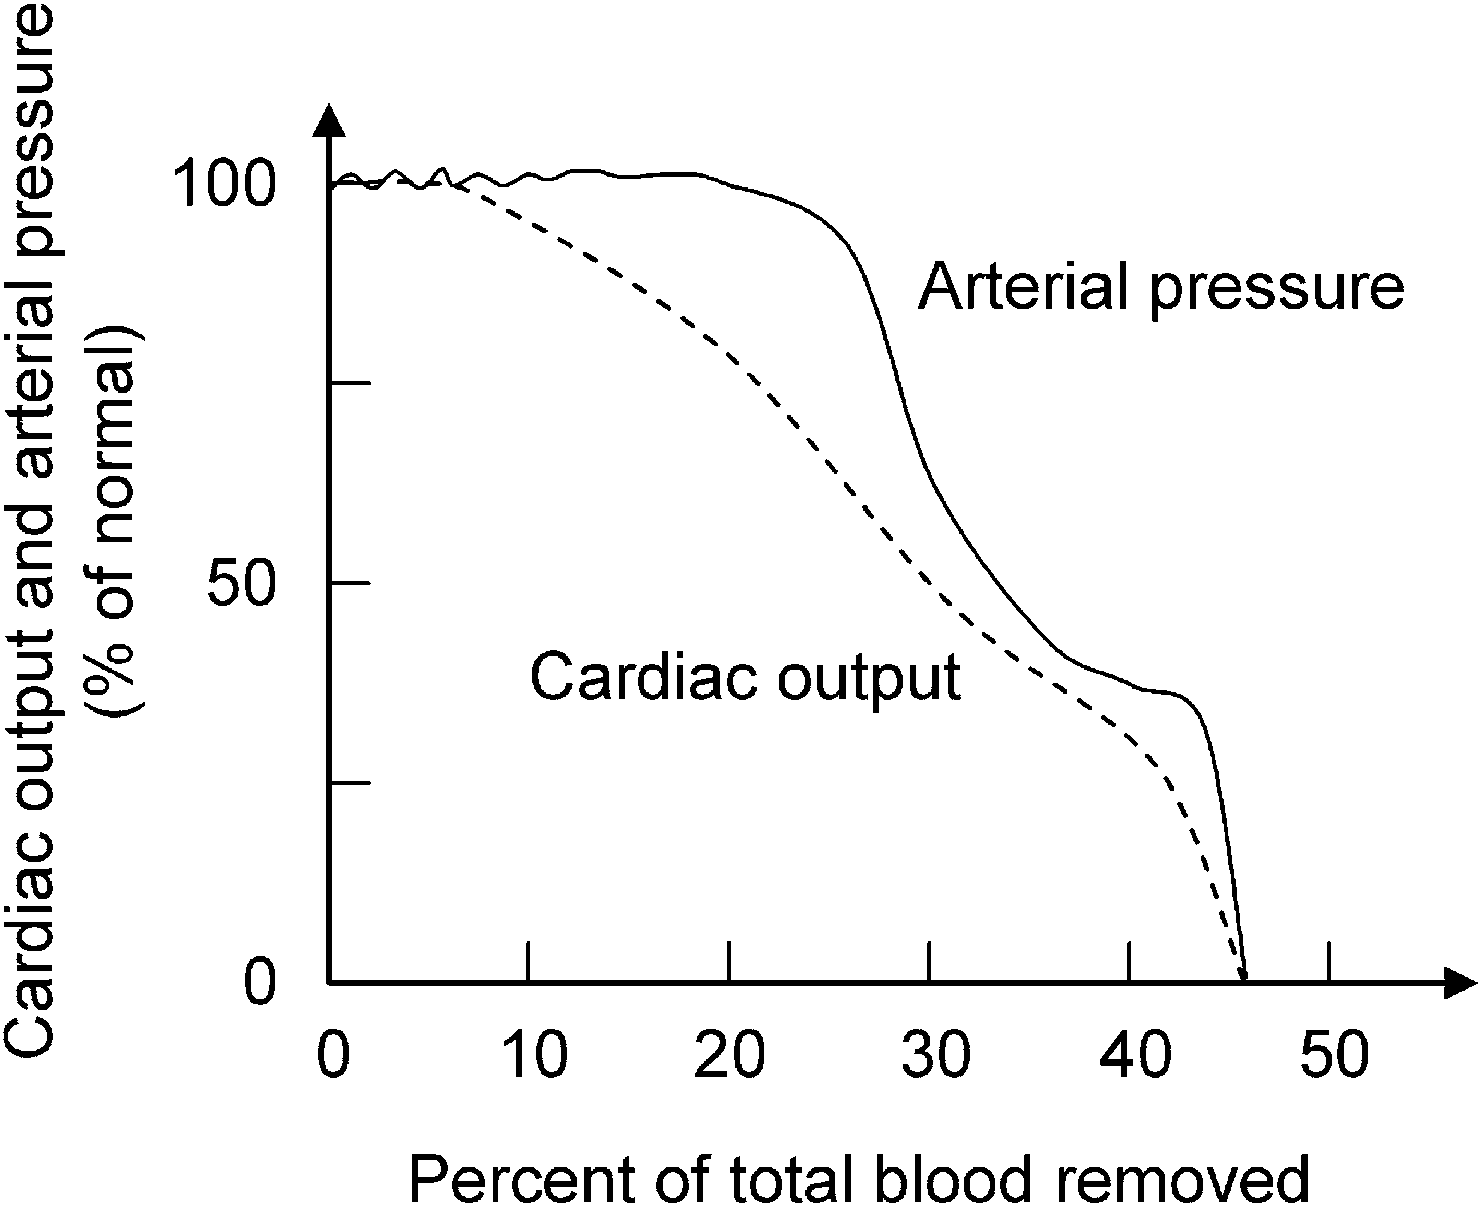
\includegraphics[width=0.55\textwidth]{835.png}
  \caption{Esquema del flujo en una arteria obstruida.}
  \label{fig:835}
\end{SCfigure}

\begin{figure}[htbp]
  \centering
  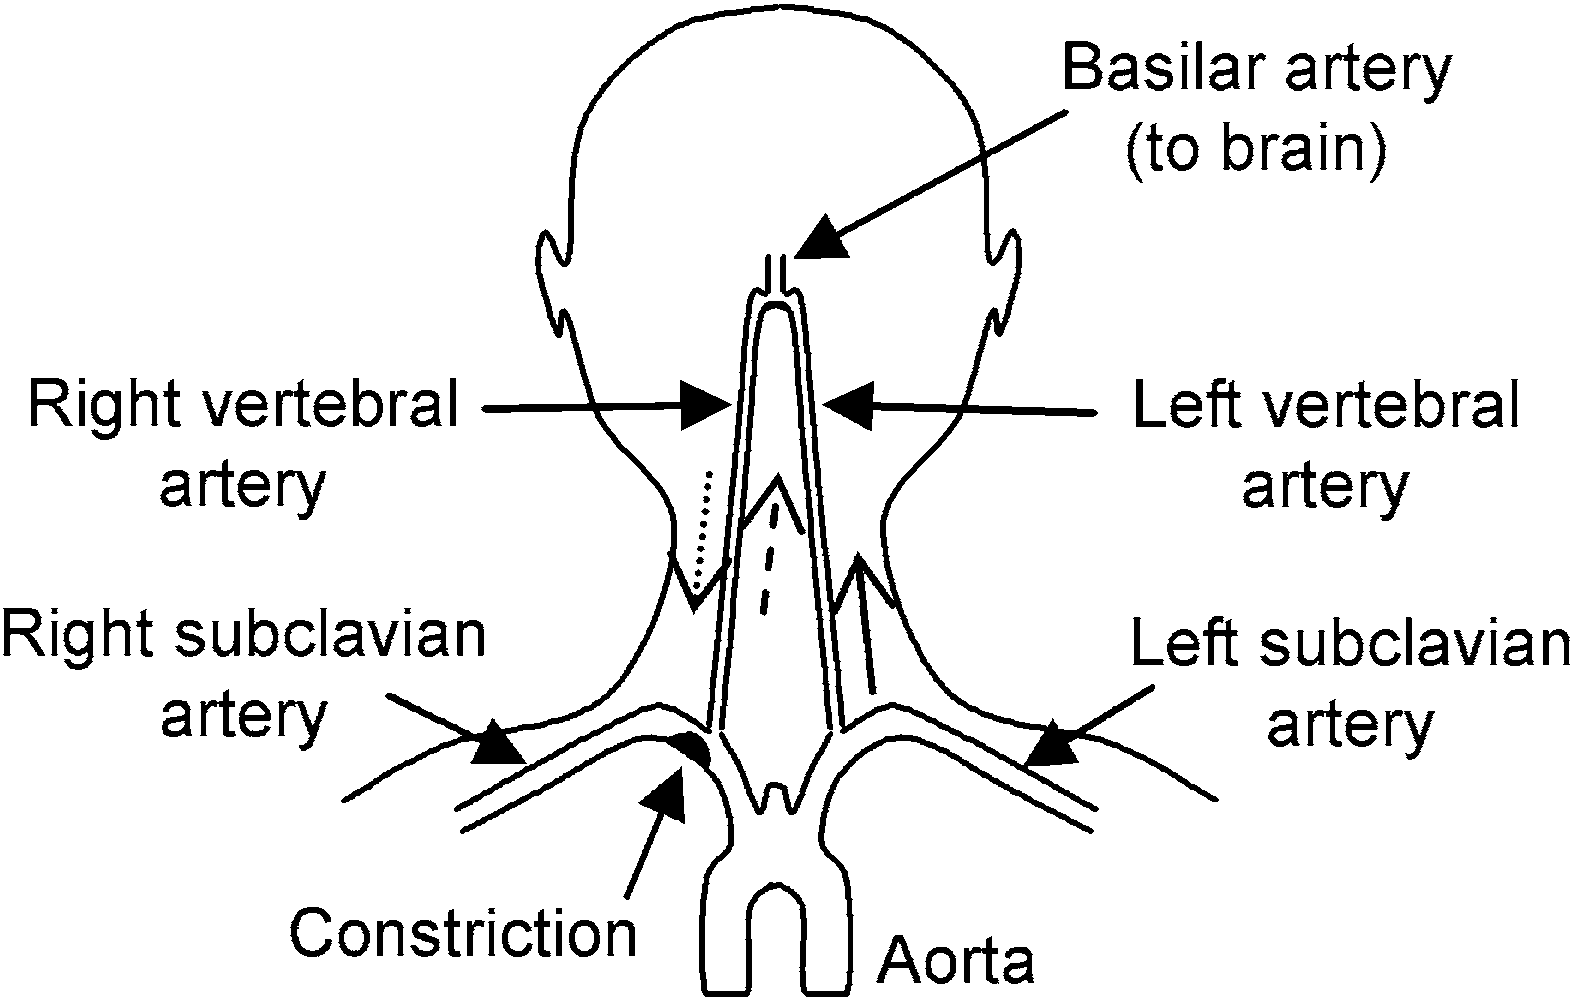
\includegraphics[width=0.7\textwidth]{836.png}
  \caption{El flujo es parcialmente turbulento en arterias obstruidas (De [21]. Adaptado de [39]. Cortesía de Robert A. Freitas Jr., Nanomedicine, Vol.~1 (1999), http://www.nanomedicine.com).}
  \label{fig:836}
\end{figure}



En 1954, Arturo Toscanini dirigía la Orquesta Sinfónica de la NBC. (Esta orquesta era muy prestigiosa en ese entonces, presentándose en la radio y en la entonces nueva televisión, pero ya no existe). Él estaba agitando vigorosamente sus brazos, como suelen hacer los directores de orquesta, y se desmayó. ¿Por qué? La ecuación (8.34) contiene la respuesta y la Fig.~8.37 ilustra el motivo. Toscanini sufrió un accidente isquémico transitorio (AIT, o \emph{TIA} por sus siglas en inglés) [26, 42]. La isquemia (is-que-mia) es la disminución local del flujo sanguíneo. El AIT es la pérdida temporal de sangre al cerebro debido al «síndrome de robo de la subclavia». Este da lugar a mareos temporales, visión doble, dolor de cabeza y debilidad en las extremidades. Por su naturaleza, es solo temporal, pero indica un problema más grave.

\begin{figure}[htbp]
  \centering
  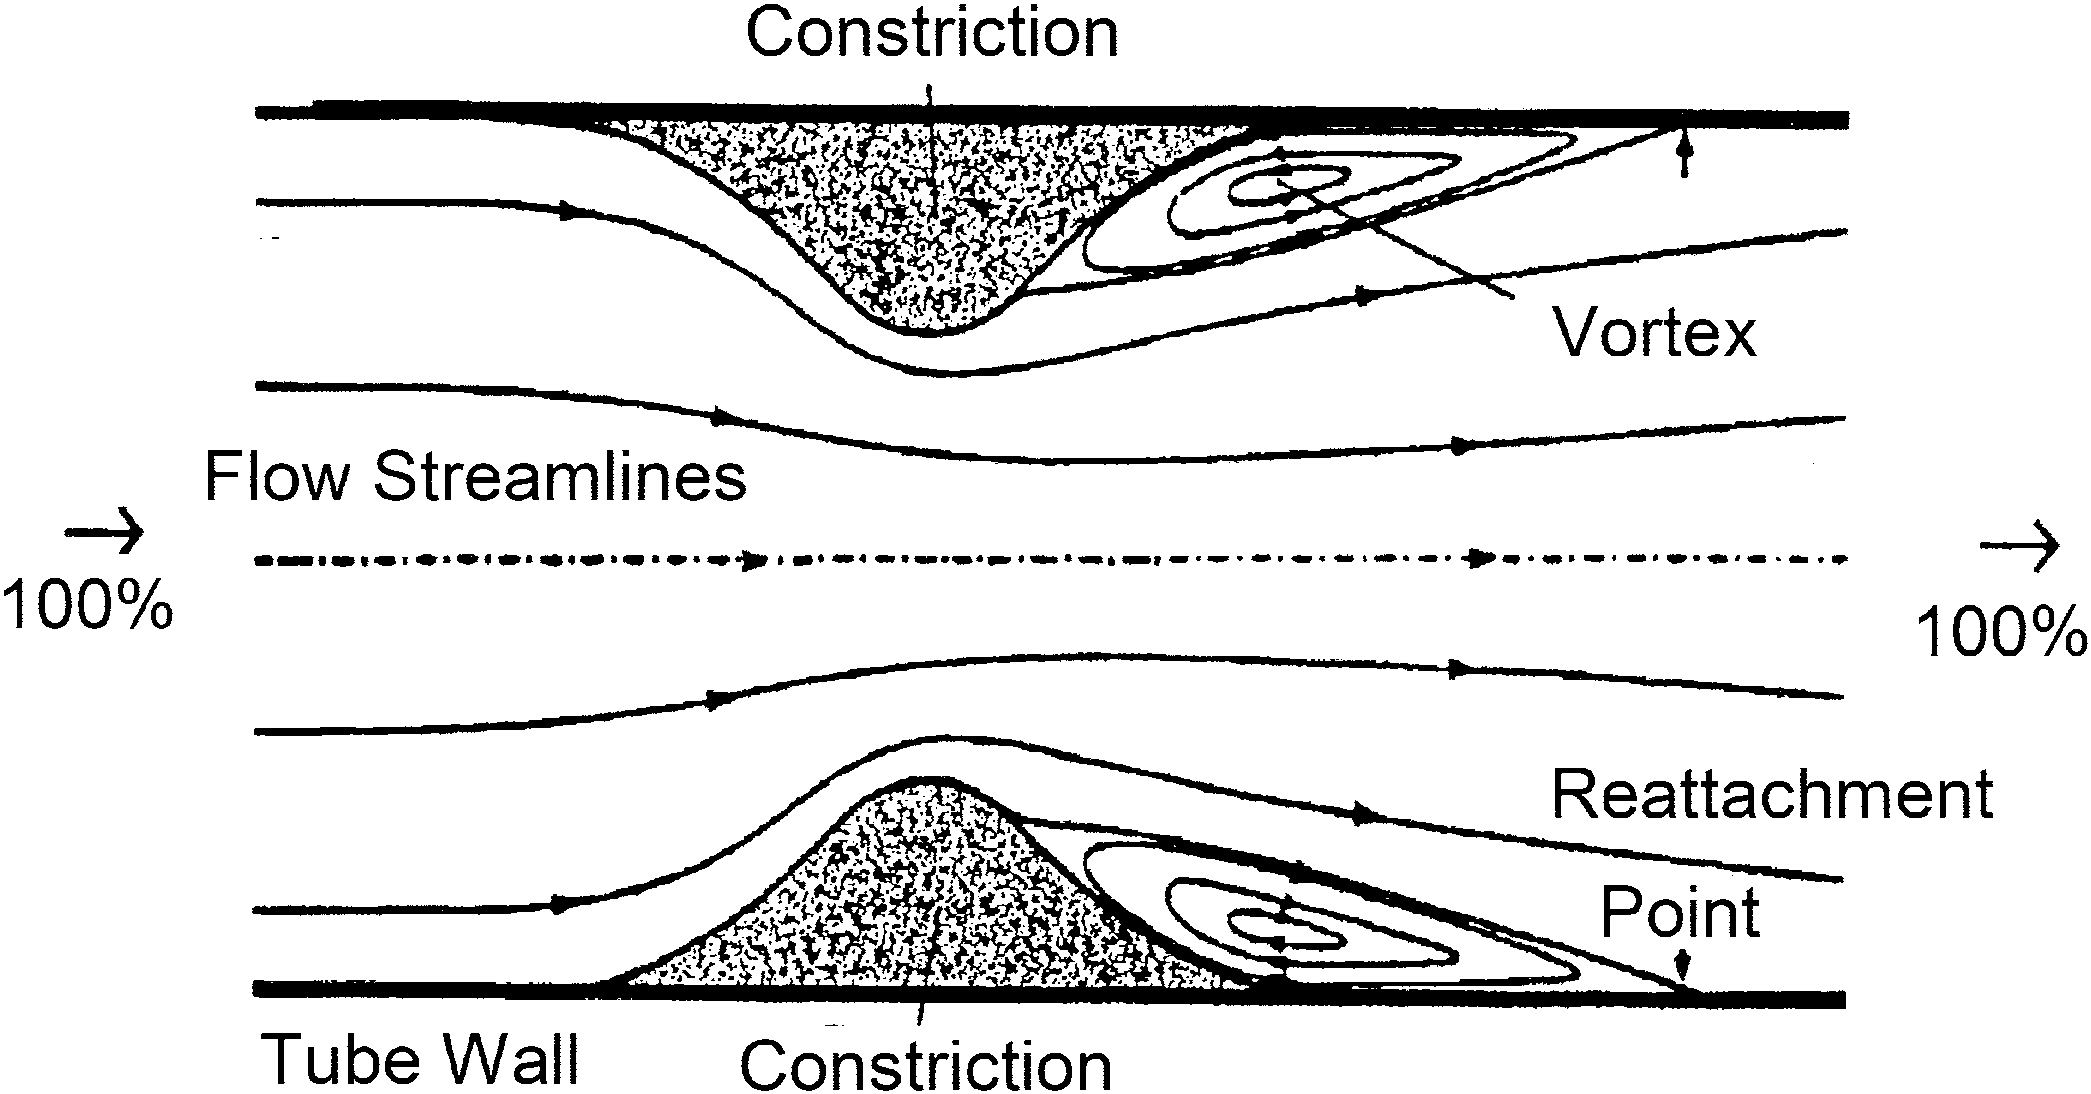
\includegraphics[width=0.8\textwidth]{837.png}
  \caption{Vista anterior del flujo sanguíneo al cerebro con el síndrome de robo de la subclavia, que da lugar a un accidente isquémico transitorio. El flujo sanguíneo en la arteria vertebral izquierda se muestra con la flecha de línea continua. Sin la constricción, el flujo sanguíneo en la arteria vertebral derecha es normal, como se muestra con la flecha discontinua, por lo que hay un flujo sanguíneo normal hacia la arteria basilar. Con la constricción, puede haber flujo sanguíneo desde la arteria vertebral izquierda hacia la arteria vertebral derecha (flecha punteada), y no hay flujo sanguíneo hacia la arteria basilar (Basado en [26]).}
  \label{fig:837}
\end{figure}



Las arterias carótidas izquierda y derecha son dos arterias principales que suministran sangre a la parte anterior del cerebro. Las arterias vertebrales izquierda y derecha suministran sangre a la parte posterior del cerebro. Estas se ramifican a partir de las arterias subclavias, las cuales también suministran sangre a los brazos. Los sistemas carotídeo interno y vertebral se unen entre sí en la base del cerebro, formando el polígono de Willis (Fig.~8.38; véase también la Fig.~8.42 más adelante). Posteriormente, el flujo en las arterias vertebrales izquierda y derecha se fusiona para formar una única arteria basilar hacia el cerebro.

\begin{figure}[htbp]
  \centering
  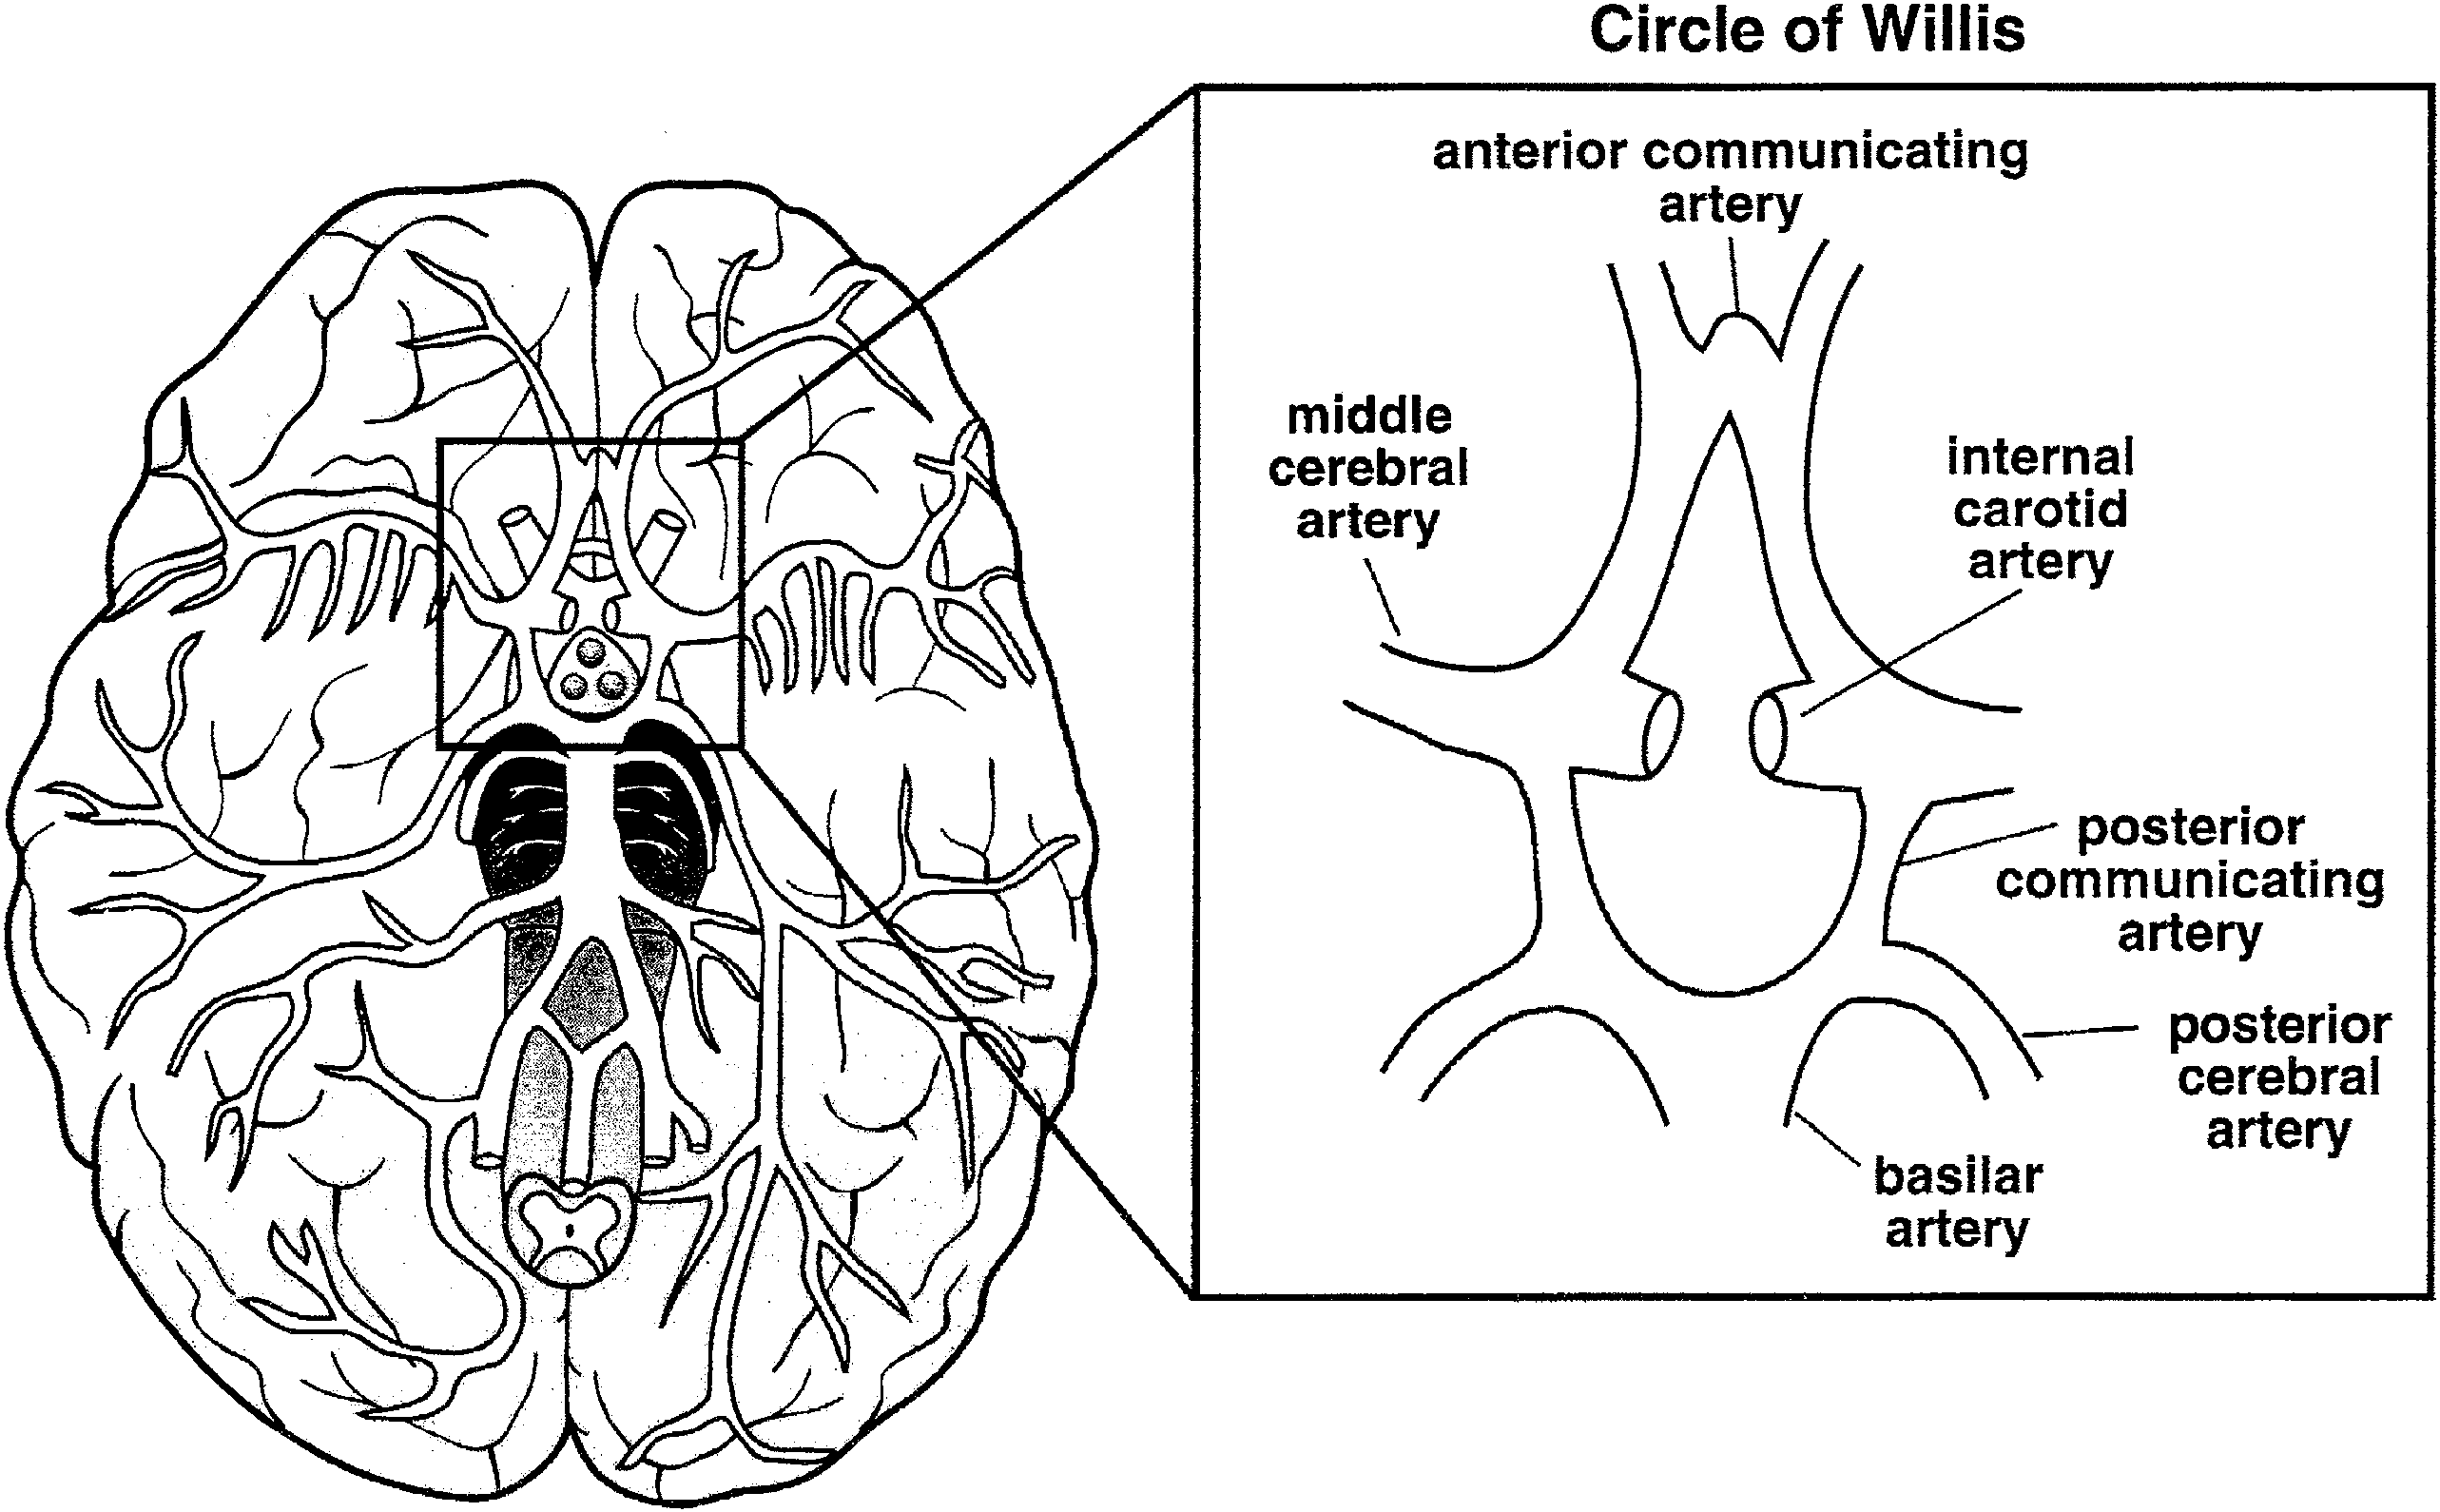
\includegraphics[width=0.8\textwidth]{838.png}
  \caption{Polígono de Willis en el cerebro (De [31]).}
  \label{fig:838}
\end{figure}

\begin{figure}[htbp]
  \centering
  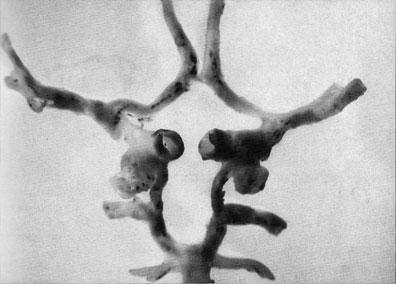
\includegraphics[width=0.7\textwidth]{842.png}
  \caption{Fotografía de una vista inferior de un polígono de Willis humano extirpado. Se observan aneurismas saculares bilaterales (es decir, en ambos lados) cerca de la unión entre la arteria carótida interna y el polígono; la lesión más grande (la del lado izquierdo de la fotografía) se había roto (De [36]).}
  \label{fig:842}
\end{figure}



Supongamos que hay una constricción en la arteria subclavia derecha cerca de donde se ramifica la arteria vertebral (Fig.~8.37). La presión antes de la constricción y en la misma región en el lado derecho normal es $P_1$. Debido a la constricción, la presión en el lado izquierdo es $P_2 < P_1$. Esta diferencia aumenta con un flujo sanguíneo más rápido. Con el movimiento vigoroso de los brazos, surge la necesidad de un mayor flujo sanguíneo en las arterias subclavias para suministrar más oxígeno al músculo esquelético de los hombros y los brazos, y la velocidad de la sangre en estas arterias, $u_1$, aumenta. Si $u_1$ aumenta lo suficiente, $P_2$ se vuelve mucho menor que $P_1$, de modo que el flujo en la arteria vertebral izquierda se desvía hacia la arteria vertebral derecha ---y no fluye hacia la arteria basilar al cerebro---. Cuando esto le sucedió a Toscanini, se desmayó. Dejó de mover las manos, por supuesto. El flujo sanguíneo a sus brazos disminuyó entonces. La diferencia entre $P_1$ y $P_2$ disminuyó a su valor menor habitual (incluso con esta constricción). La sangre de ambas arterias vertebrales fluyó entonces a su arteria basilar. Su cerebro comenzó a recibir un flujo normal de sangre de nuevo y recuperó el conocimiento. Todo estaba bien, pero esta constricción tenía que ser eliminada. (Toscanini nunca volvió a dirigir. La razón subyacente de su desmayo no se conocía en 1954; el AIT se explicó por primera vez en 1961).

¿Cómo se forman tales obstrucciones? Las lipoproteínas de baja densidad (LDL, o colesterol malo) transportan el colesterol y los triglicéridos desde el hígado a otros órganos. Estas son el material de construcción para formar la placa en las paredes arteriales que conduce a la aterosclerosis (enfermedad cardíaca). Las lipoproteínas de alta densidad (HDL, o colesterol bueno) parecen ayudar a disolver la placa y llevar el colesterol de regreso al hígado. La historia completa es compleja y actualmente no está clara, pero está claro que una buena dieta y el ejercicio (así como buenos genes) parecen ayudar a disminuir la formación neta de placa y las enfermedades cardíacas [6]. (Una buena dieta y el ejercicio, además de buenos genes, parecen evitar el veredicto grave para muchas enfermedades potenciales). Los ácidos grasos insaturados, tales como los provenientes del pescado y los frutos secos, tienen menos átomos de hidrógeno debido a que no todos los enlaces carbono-carbono son enlaces simples, y son líquidos a temperatura ambiente. Estos parecen hacer que el hígado forme HDL. Los ácidos grasos saturados, tales como los de la carne roja, tienen más átomos de hidrógeno debido a que todos los enlaces carbono-carbono son enlaces simples, y son sólidos a temperatura ambiente. Estos parecen hacer que el hígado forme LDL. Las grasas insaturadas que han sido convertidas industrialmente en grasas saturadas, las grasas trans, elevan los niveles de LDL y disminuyen los de HDL [44].

Más adelante en este capítulo se examinarán más ejemplos de los efectos de las obstrucciones en las arterias.

\subsection{Trabajo realizado por el corazón y necesidades metabólicas del corazón}

Considere el ventrículo izquierdo, el cual es una bomba durante la sístole, como se esquematiza en la Fig.~8.39.

\begin{figure}[htbp]
  \centering
  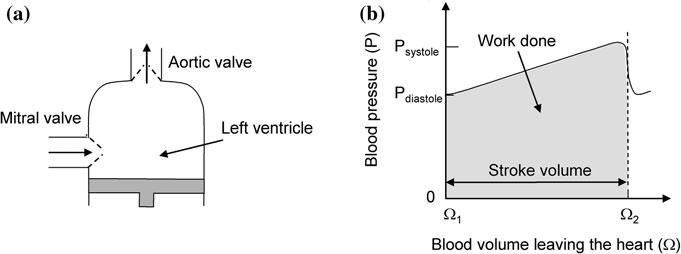
\includegraphics[width=0.8\textwidth]{839.png}
  \caption{a) Esquema del ventrículo izquierdo del corazón como una bomba, b) y la presión y el volumen del ventrículo izquierdo durante la contracción sistólica durante la sístole (desde $t_1$ a $t_2$), mostrando el trabajo realizado por el corazón (área sombreada) (Basado en [4]).}
  \label{fig:839}
\end{figure}



El trabajo es realizado por esta bomba, con una fuerza que empuja el pistón desde las posiciones inicial a final, $L_{\text{i}}$ a $L_{\text{f}}$, para obtener
\begin{equation}
W = \int_{L_{\text{i}}}^{L_{\text{f}}} F \mathrm{d}L = \int_{L_{\text{i}}}^{L_{\text{f}}} (F/A)(A \mathrm{d}L) = \int_{V_{\text{i}}}^{V_{\text{f}}} P \mathrm{d}V,
\label{eq:835}
\end{equation}
donde la fuerza/área es la presión, $P$, y la distancia multiplicada por el área es el volumen ventricular, $V$. Durante la sístole, la presión ventricular aumenta desde un valor muy bajo (el de la aurícula izquierda) hasta $P_{\text{di\'{a}stole}} \approx 80\text{ mmHg}$ (en el tiempo $t_1$), y luego hasta $P_{\text{s\'{i}stole}} \approx 120\text{ mmHg}$, y permanece en este valor hasta el final de la sístole (en el tiempo $t_2$). La válvula aórtica se abre por primera vez cuando esta presión se eleva por encima de $P_{\text{di\'{a}stole}}$ (en $t_1$), y la sangre es expulsada hasta que termina la sístole (en $t_2$). En $t_1$, el volumen de sangre bombeada es $\Omega_{\text{i}} = 0$ y en $t_2$ es $\Omega_{\text{f}} = V_{\text{i}} - V_{\text{f}}$. La Figura~8.39 muestra esta evolución de la presión ventricular y el volumen bombeado desde $t_1$ a $t_2$.

El área bajo esta curva es el trabajo realizado y, por lo tanto, $W = P_{\text{av}} V_{\text{stroke}}$, donde $P_{\text{av}}$ es la presión promedio durante este ciclo (promediada sobre el volumen desplazado y la cual no necesariamente escala linealmente con el tiempo, y asumiendo que no hay contrapresión), y $V_{\text{stroke}} = \Omega_{\text{f}}$ es el volumen sistólico. Claramente, $P_{\text{di\'{a}stole}} < P_{\text{av}} < P_{\text{s\'{i}stole}}$. Para una variación lineal, vemos que $P_{\text{av}} = (P_{\text{di\'{a}stole}} + P_{\text{s\'{i}stole}})/2 \approx 100\text{ mmHg} = 1{,}3 \times 10^4\text{ N/m}^2$. (Este promedio es diferente al de (8.1) debido a la simplicidad de este modelo. Esto conduce a una incertidumbre de ${\sim}20\%$). Tomamos $V_{\text{stroke}} = 80\text{ cm}^3 = 8 \times 10^{-5}\text{ m}^3$, por lo que $W = (1{,}3 \times 10^4\text{ N/m}^2)(8 \times 10^{-5}\text{ m}^3) = 1{,}04\text{ J}$ por ciclo. Con una frecuencia cardíaca de $60\text{/min} = 1\text{/s}$, la tasa a la que el ventrículo izquierdo realiza trabajo es $P_{\text{power,mech,av}} = (1{,}04\text{ J por ciclo})(1\text{ ciclo/s}) = 1{,}04\text{ W}$.

La eficiencia, $\epsilon$, de conversión de la energía metabólica en este trabajo mecánico es de aproximadamente el $20\%$ (y a veces este rango se da como $12\text{--}30\%$), por lo que la potencia metabólica necesaria para hacer funcionar el ventrículo izquierdo es $P_{\text{power,metab,av}} = P_{\text{power,mech,av}}/\epsilon = 5\text{ W}$.

El corazón bombea durante aproximadamente $1/3$ del ciclo cardíaco y descansa durante el otro $2/3$ del tiempo. Por lo tanto, las potencias de pico son mayores que estos valores promedio por un factor de $3$, con $P_{\text{power,mech,peak}} = 1{,}5\text{ W}$ y $P_{\text{power,metab,peak}} = 15\text{ W}$.

La energía consumida para hacer funcionar el ventrículo izquierdo es $(86\,400\text{ s/d\'{i}a})(5\text{ W}) = 4{,}32 \times 10^5\text{ J/d\'{i}a} = 104\text{ kcal/d\'{i}a}$. Hasta ahora hemos examinado únicamente el trabajo realizado por el ventrículo izquierdo. El ventrículo derecho bombea el mismo volumen por ciclo cardíaco (para mantener el flujo en estado estacionario en todo momento), pero a una presión $1/5$ veces la del ventrículo izquierdo, por lo que el trabajo y todas estas potencias son menores por un factor de cinco. Esto aumenta la potencia metabólica requerida en un $20\%$. De manera similar, las presiones para las dos aurículas también son relativamente muy pequeñas. En general, con una eficiencia muscular del $20\%$, esperamos necesitar ${\sim}125\text{ kcal/d\'{i}a}$ para hacer funcionar el corazón; con una eficiencia muscular del $10\%$, serían ${\sim}250\text{ kcal/d\'{i}a}$.

El valor experimental para la contribución al BMR de todo el corazón es de ${\sim}117\text{ kcal/d\'{i}a}$ (Tabla~6.17), lo cual está cerca de nuestra estimación. La mayor incertidumbre aquí es la eficiencia del músculo cardíaco.

¿Qué sucede con el ejercicio extenuante? La presión arterial puede aumentar en un $50\%$ y la tasa de flujo sanguíneo puede aumentar en un factor de $5$. Por lo tanto, la potencia mecánica ejercida por el corazón y los requisitos metabólicos asociados pueden aumentar en un factor de $7{,}5$.

\section{Accidentes cerebrovasculares y aneurismas}

La sangre cerebral fluye desde las arterias carótidas internas y vertebrales y a través del polígono de Willis en la base del cerebro (Fig.~8.38), y luego impregna el cerebro a través de una serie compleja de capilares.

Cualquier restricción severa de sangre al cerebro se denomina accidente cerebrovascular [30, 31]. La isquemia significa que hay una falta de flujo sanguíneo. El tejido cercano se vuelve deficiente en oxígeno y metabolitos, y presenta un exceso de productos de desecho metabólicos. (Vimos un ejemplo de isquemia anteriormente en este capítulo con el AIT de Toscanini. Debido a que el AIT es transitorio, existe una deficiencia de oxígeno debido al accidente cerebrovascular, pero el paciente aún puede recuperarse con poco o ningún daño cerebral). La hipoxia significa una falta de oxígeno, y puede resultar de la isquemia o de otras causas, como la gran altitud (véase el Cap.~9) o la intoxicación por CO. El infarto significa que el accidente cerebrovascular causa daño cerebral permanente. (Los términos isquemia e infarto son en realidad más generales y también se aplican a tejidos fuera del cerebro, siendo un ejemplo el infarto de miocardio en el corazón). La transición del evento reversible al infarto irreversible con la formación de tejido necrótico ocurre cuando el accidente cerebrovascular es particularmente prolongado o de magnitud particularmente grande. (El tejido necrótico es tejido muerto que no murió de la manera programada por el cuerpo, por lo que contrasta con el tejido apoptótico, el cual es eliminado por el cuerpo como parte de su ciclo vital). La aparición de un accidente isquémico transitorio, o microinfarto, a veces significa que un accidente cerebrovascular más dañino es inminente. A continuación, abordaremos los accidentes cerebrovasculares hemorrágicos e isquémicos, los cuales se deben a la ruptura y obstrucción de los vasos sanguíneos, respectivamente.

\subsection{Accidentes cerebrovasculares hemorrágicos}

Los accidentes cerebrovasculares hemorrágicos se deben a la ruptura de la vasculatura (vasos sanguíneos) dentro del cerebro, atribuida a un aneurisma o a un vaso sanguíneo debilitado (Fig.~8.40). Un aneurisma es un vaso sanguíneo agrandado. Además de la pérdida de sangre en las regiones de destino, durante las hemorragias la sangre llena los espacios circundantes y comprime los tejidos aledaños. Esta sangre acumulada comprime otros vasos sanguíneos, disminuyendo sus diámetros y reduciendo el flujo de sangre a otras partes del cerebro, e incrementa la presión intracraneal, lo que conduce a complicaciones neurológicas. Alrededor del $20\%$ de todos los accidentes cerebrovasculares son hemorrágicos; ocurren principalmente en jóvenes y personas de mediana edad debido a lesiones vasculares tales como malformaciones arteriovenosas y aneurismas. (Las lesiones son entidades de tejido enfermo o anormal). En los ancianos, los vasos sanguíneos son frágiles y menos distensibles debido a los depósitos ateroscleróticos, y esto puede conducir a una posible ruptura espontánea de estos vasos en el cerebro y a un accidente cerebrovascular hemorrágico. En la aterosclerosis («endurecimiento de las arterias»), los depósitos lipídicos o grasos en la sangre se acumulan en la pared interna del vaso y finalmente forman una placa arterial dura.

\begin{SCfigure}[0.9][htbp]
  \centering
  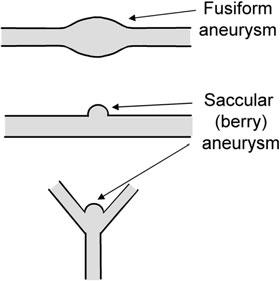
\includegraphics[width=0.5\textwidth]{840.png}
  \caption{Aneurismas fusiformes y saculares/en baya, este último en un vaso y para flujo bifurcado.}
  \label{fig:840}
\end{SCfigure}



La mayoría de los aneurismas cerebrales son aneurismas saculares (o en forma de baya) que ocurren con mayor frecuencia donde las arterias cerebrales grandes se bifurcan (Figs.~8.41 y 8.42). En los aneurismas fusiformes hay una dilatación uniforme de la circunferencia de las paredes del vaso, en lugar de en regiones localizadas de los vasos como en los aneurismas saculares; esto conduce a aneurismas elipsoidales o con forma de balón de fútbol americano. (Fusiforme significa que se estrecha en cada extremo. Aquí indica un aneurisma cilíndricamente simétrico que se estrecha hacia el vaso normal en cualquiera de los extremos, mientras que para los músculos fusiformes en el Cap.~5 indica un músculo cilíndricamente simétrico que se estrecha hacia tendones en cada extremo). Los aneurismas fusiformes son menos comunes en el cerebro que los aneurismas saculares, pero son comunes en otras partes del cuerpo. El aneurisma de aorta abdominal, que se desarrolla a lo largo de la aorta en la región abdominal o intestinal, es el aneurisma más común que se encuentra en el cuerpo y es un aneurisma fusiforme (Fig.~8.43).

\begin{figure}[htbp]
  \centering
  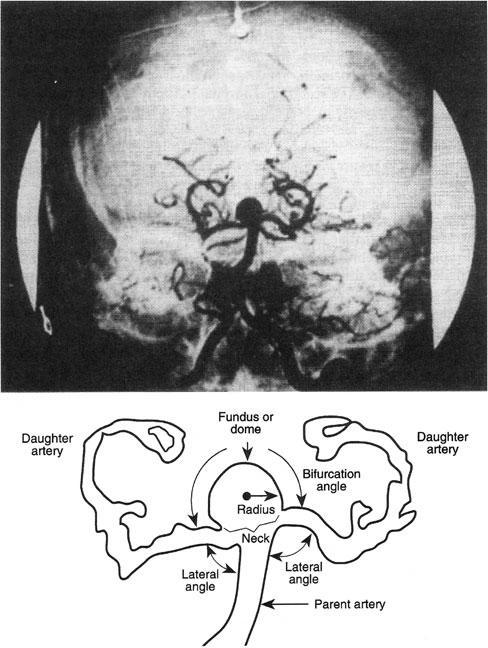
\includegraphics[width=0.45\textwidth]{841.png}
  \caption{Aneurisma sacular (en baya) en el vértice de un vaso ramificado, mostrando una imagen de proyección angiográfica (arriba) y un modelo (abajo) (De [31]).}
  \label{fig:841}
\end{figure}

\begin{figure}[htbp]
  \centering
  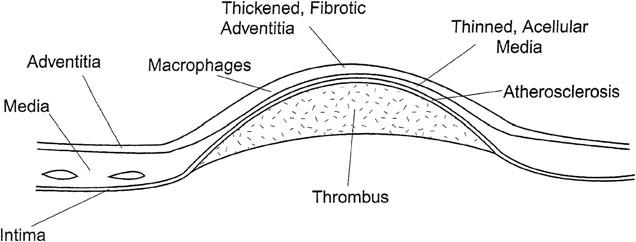
\includegraphics[width=0.8\textwidth]{843.png}
  \caption{Esquema de un aneurisma de aorta abdominal, mostrando una capa media atenuada y un trombo intraluminal (De [36]).}
  \label{fig:843}
\end{figure}



Las arterias sanas contienen las proteínas estructurales elastina y colágeno. El colágeno tiene el módulo de Young más grande (Tabla~4.2) y se espera que domine las propiedades elásticas de las arterias. Aún así, la elastina contribuye a la distensibilidad de la arteria. La resistencia al estiramiento a presiones bajas parece deberse a las fibras de elastina, a presiones fisiológicas normales se debe a las fibras de elastina y colágeno, y a presiones aún más altas se debe al colágeno. Cuando la pared de la arteria se dilata o se saculiza (es decir, se dilata en una parte circunferencial de la pared) a medida que se desarrolla el aneurisma, la elastina se vuelve menos eficaz para mantener la integridad estructural de la arteria y el colágeno asume la mayor parte de la carga. La arteria se vuelve menos distensible y esto se traduce en un mayor esfuerzo para la misma deformación, acelerando así la fatiga estructural. Este proceso acelera la carga sobre la pared arterial y conduce a la ruptura. En la Fig.~8.44 se muestra un escenario posible para la formación y ruptura de un aneurisma sacular. La Figura~8.45 muestra la tensión circunferencial de equilibrio para un vaso asumiendo la ley de Laplace, para una arteria normal y para una con un aneurisma. La Figura~7.11 muestra que la velocidad máxima del flujo sanguíneo se encuentra en el centro, donde el esfuerzo de corte en la pared es mínimo. La velocidad mínima del flujo sanguíneo se encuentra cerca de la pared, donde el esfuerzo de corte en la pared es máximo.

\begin{figure}[htbp]
  \centering
  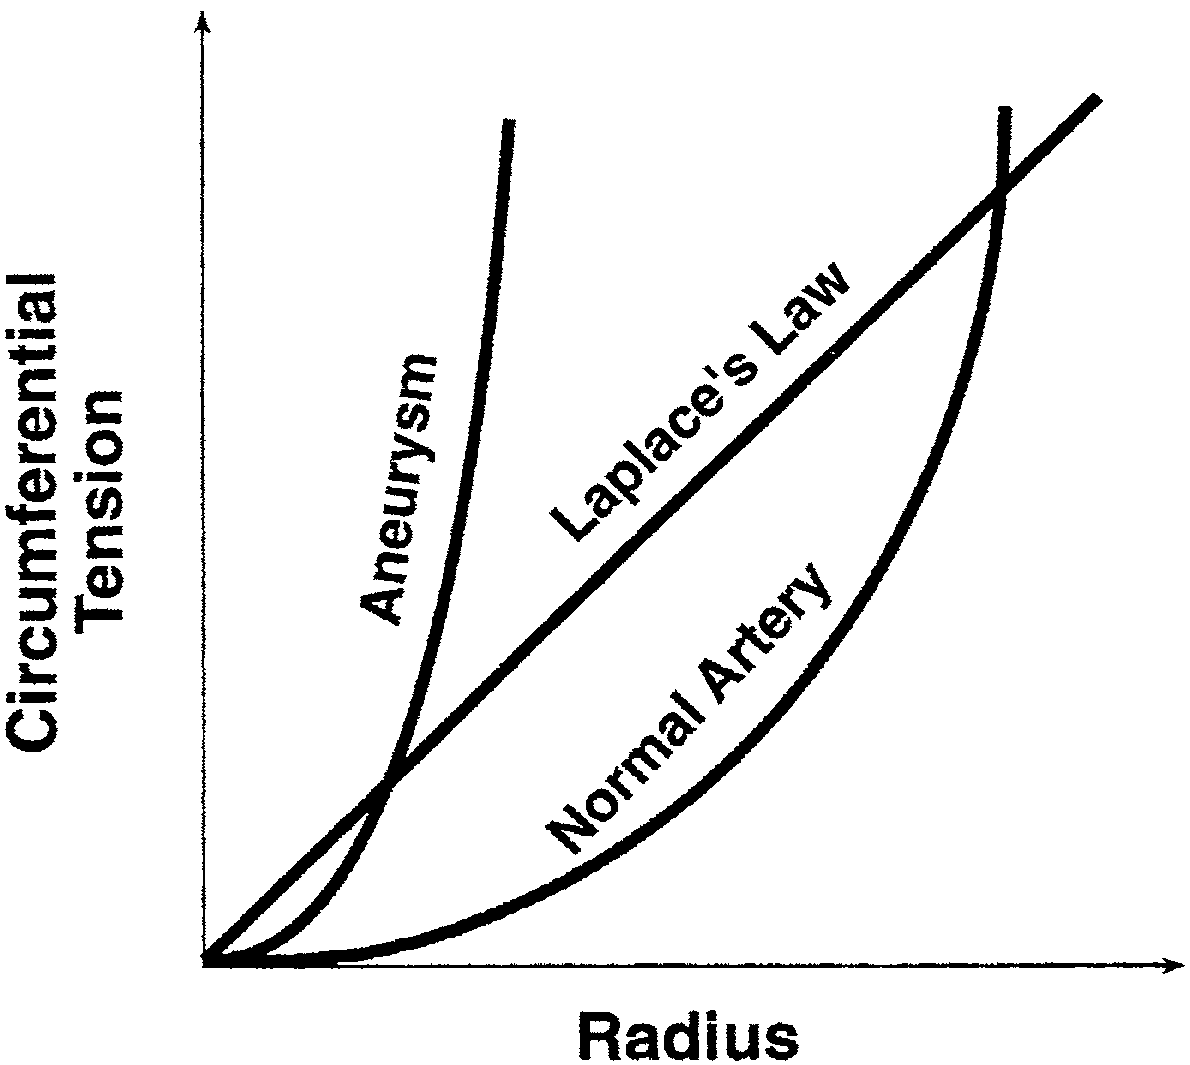
\includegraphics[width=0.7\textwidth]{844.png}
  \caption{Una posible historia natural para el desarrollo de un aneurisma sacular. Un debilitamiento local de la pared del vaso, que conduce a una leve dilatación, puede ser causado por una «injuria» inicial debido a una de varias causas (De [36]).}
  \label{fig:844}
\end{figure}

\begin{SCfigure}[0.8][htbp]
  \centering
  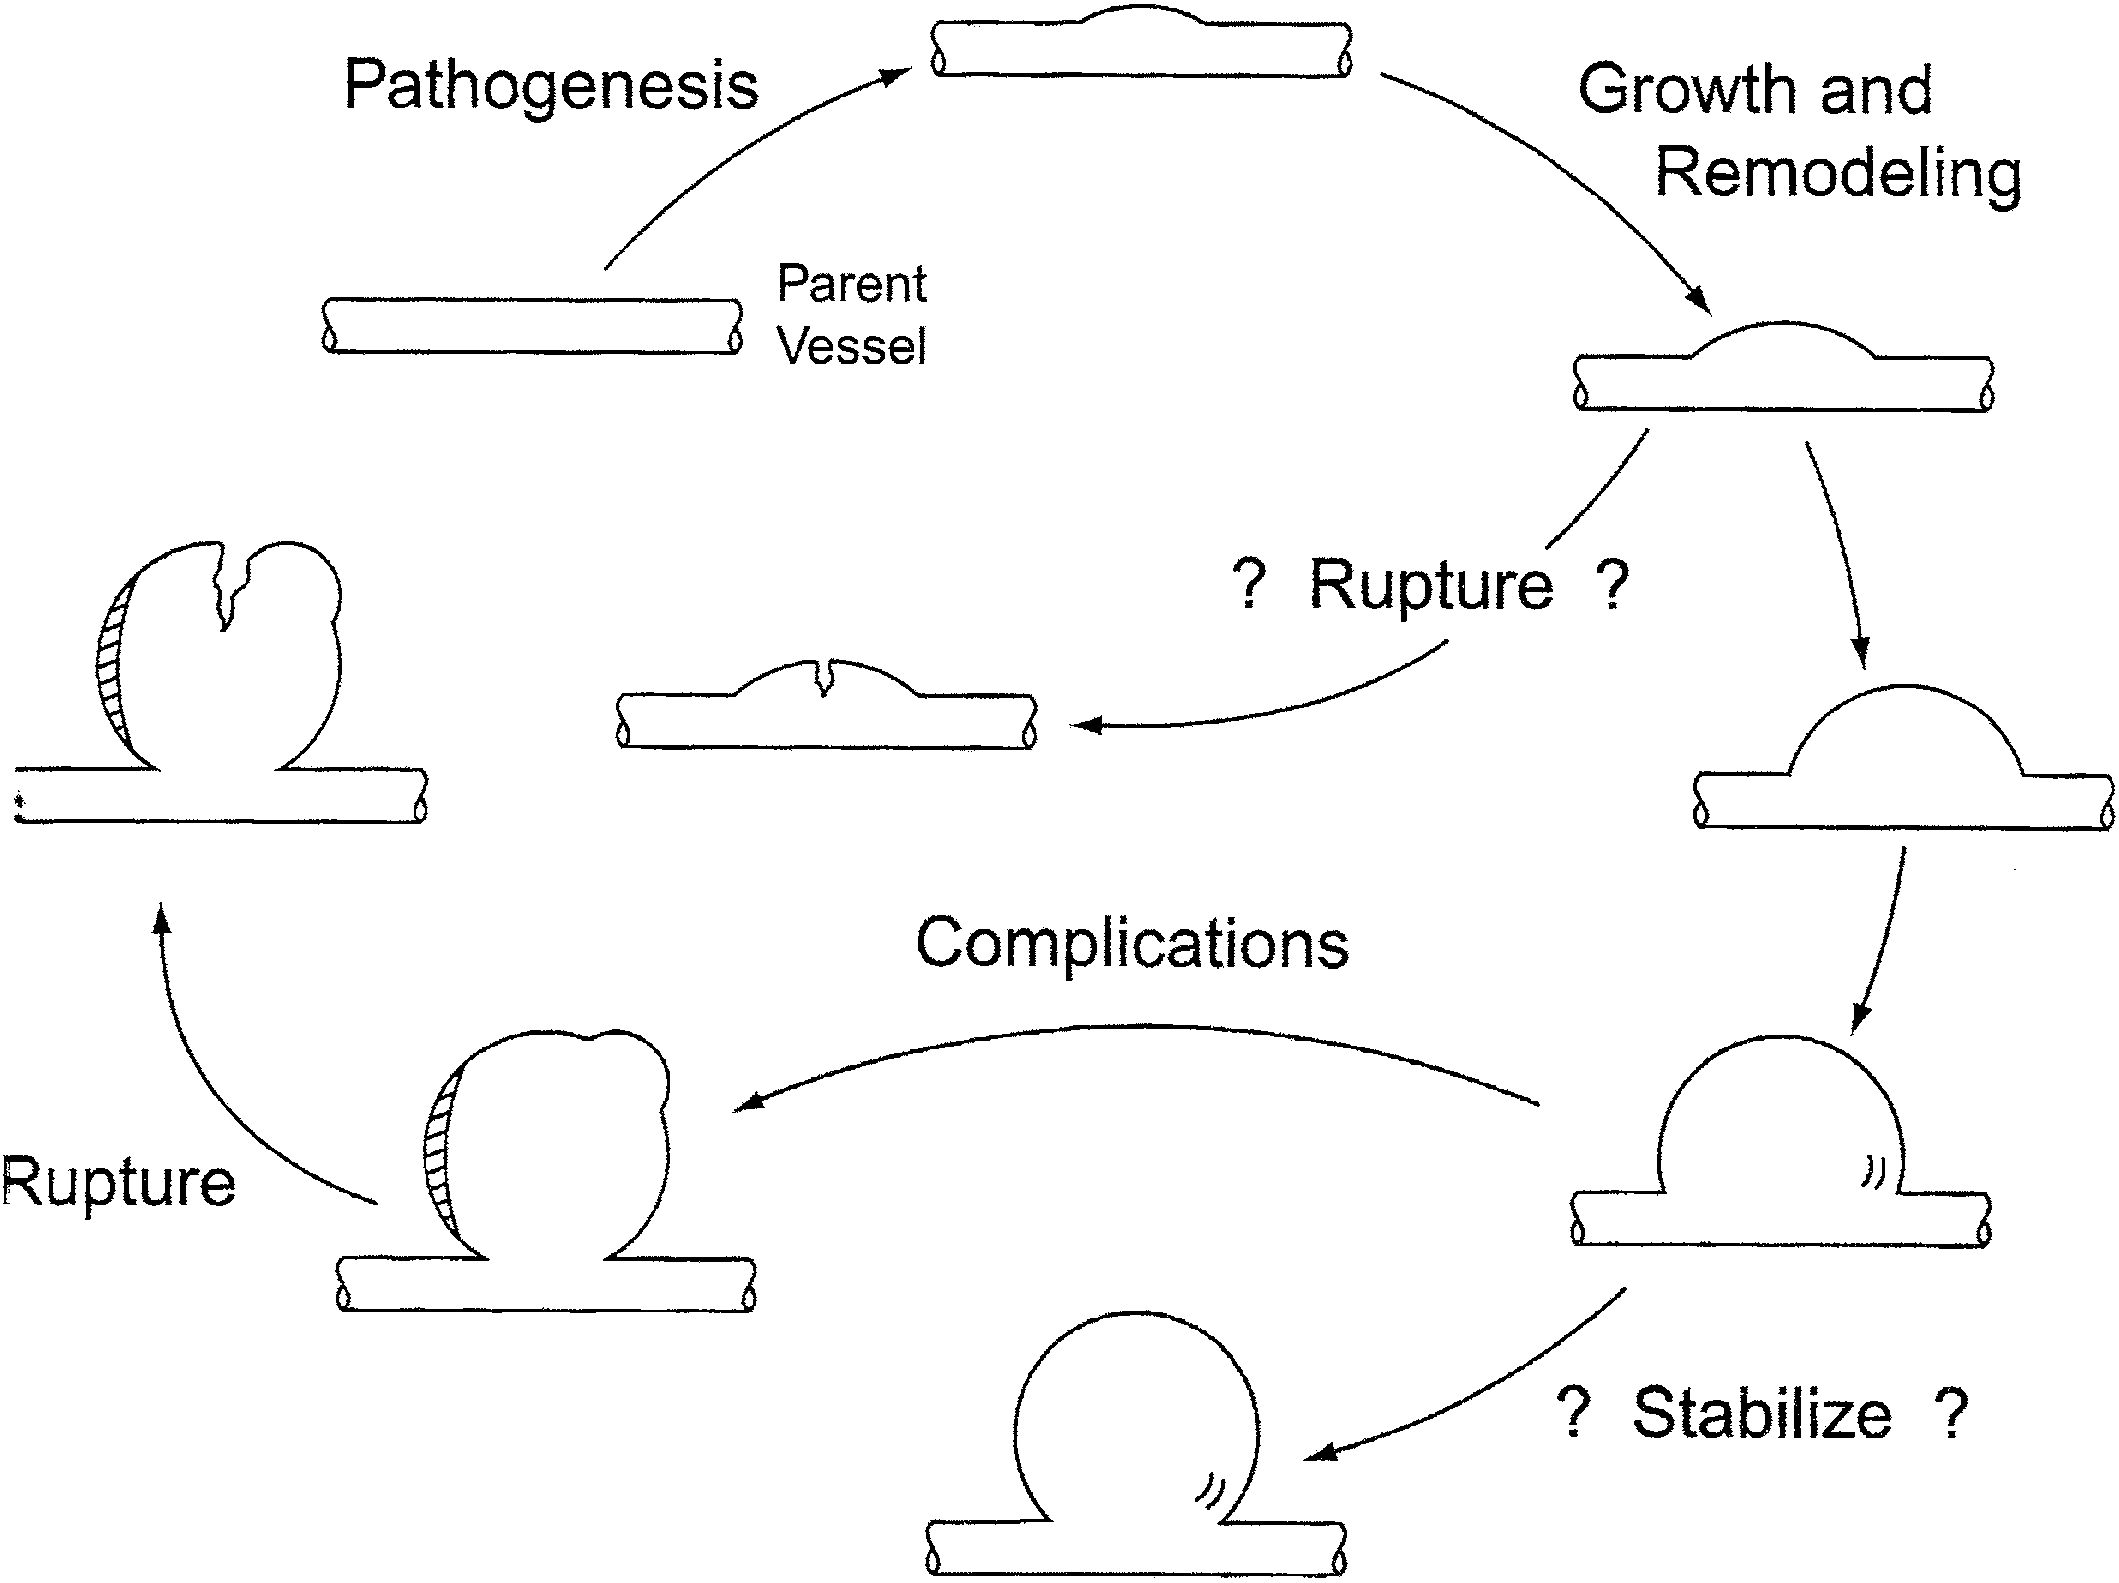
\includegraphics[width=0.55\textwidth]{845.png}
  \caption{Tensión circunferencial necesaria para el equilibrio como función del radio del vaso, asumiendo la ley de Laplace, una arteria normal y una arteria con un aneurisma (De [31, 32]).}
  \label{fig:845}
\end{SCfigure}



Existen (al menos) cuatro razones físicas por las cuales el radio más grande de un aneurisma fusiforme puede conducir a la ruptura. Todas están relacionadas con la relación de esfuerzo $T/w = r\Delta P / w$, utilizando la ley de Laplace para un cilindro (7.4), donde $w$ es el espesor de la pared y $r$ es el radio local del vaso. (1) $r$ es más grande, por lo que se necesita más tensión para soportar incluso una diferencia de presión sin cambios (debido a que $T = r\Delta P$). (2) Este aumento en el radio del vaso puede ir acompañado de un adelgazamiento de las paredes (si el volumen de la pared del vaso por unidad de longitud, ${\sim}2\pi r w$, permanece relativamente sin cambios por el aneurisma), por lo que el esfuerzo $T/w$ aumenta aún más. (3) Con este adelgazamiento de la pared puede haber daños que reduzcan localmente el UTS, y el UTS debe ser $\gg T/w$ para evitar la ruptura. (4) Un $r$ mayor, y el consecuente mayor área de sección transversal $A$, conduce a una menor velocidad de la sangre $u$, a través de la continuidad volumétrica (7.16). Esto a su vez conduce a una mayor presión $P$, a través de la ecuación de Bernoulli (7.18). Esto aumenta la tensión que debe soportar el vaso. Las magnitudes de varios de estos efectos se evalúan en el Problema~8.38.

Las tres primeras razones también se aplican a los aneurismas saculares, tras reemplazar la ley de Laplace para un cilindro por la de una esfera (7.9).

\subsubsection*{Bifurcaciones arteriales y formación de aneurismas saculares}

Dos de las razones para la formación de aneurismas saculares son las fuerzas sobre las paredes arteriales causadas por el cambio de cantidad de movimiento (como el efecto de manguera de bomberos en arterias curvas) y el esfuerzo cortante. La Figura~8.46 representa una arteria «madre» (o principal) con un área de sección transversal $A_1$ en la cual la sangre fluye a una velocidad promedio $u_1$, la cual se divide en dos vasos «hijos» (o ramas) a un ángulo $\theta$ con respecto a la madre (y $2\theta$ entre sí). (El semiángulo se muestra como $\theta_2$ en la figura). Cada vaso hijo tiene un área de sección transversal $A_2$ y una velocidad de la sangre $u_2$. El ángulo $2\theta$ usualmente varía de $30$ a $120^\circ$ (véanse también los Problemas 8.34 a 8.37). El vértice de la bifurcación (Fig.~8.46) es el sitio de máximo esfuerzo debido al impacto, deflexión y separación del flujo, y a la posible formación de turbulencias y vórtices (Fig.~8.47). La conservación del caudal $Q$ (flujo de volumen/tiempo) significa
\begin{equation}
Q = u_1 A_1 = 2 u_2 A_2.
\label{eq:836}
\end{equation}
En estos vasos, usualmente $2 A_2 > A_1$, por lo que $u_2 < u_1$.

\begin{figure}[htbp]
  \centering
  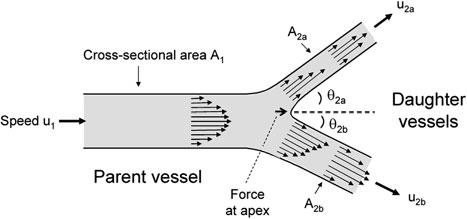
\includegraphics[width=0.8\textwidth]{846.png}
  \caption{Diagrama de una bifurcación asimétrica en un vaso, con un ángulo de bifurcación $\theta_{2\text{a}} + \theta_{2\text{b}}$. Para la bifurcación simétrica descrita en el texto, se pueden ignorar las etiquetas «a» y «b», y el semiángulo se denomina $\theta$ (Véanse los Problemas 8.34 a 8.37).}
  \label{fig:846}
\end{figure}

\begin{figure}[htbp]
  \centering
  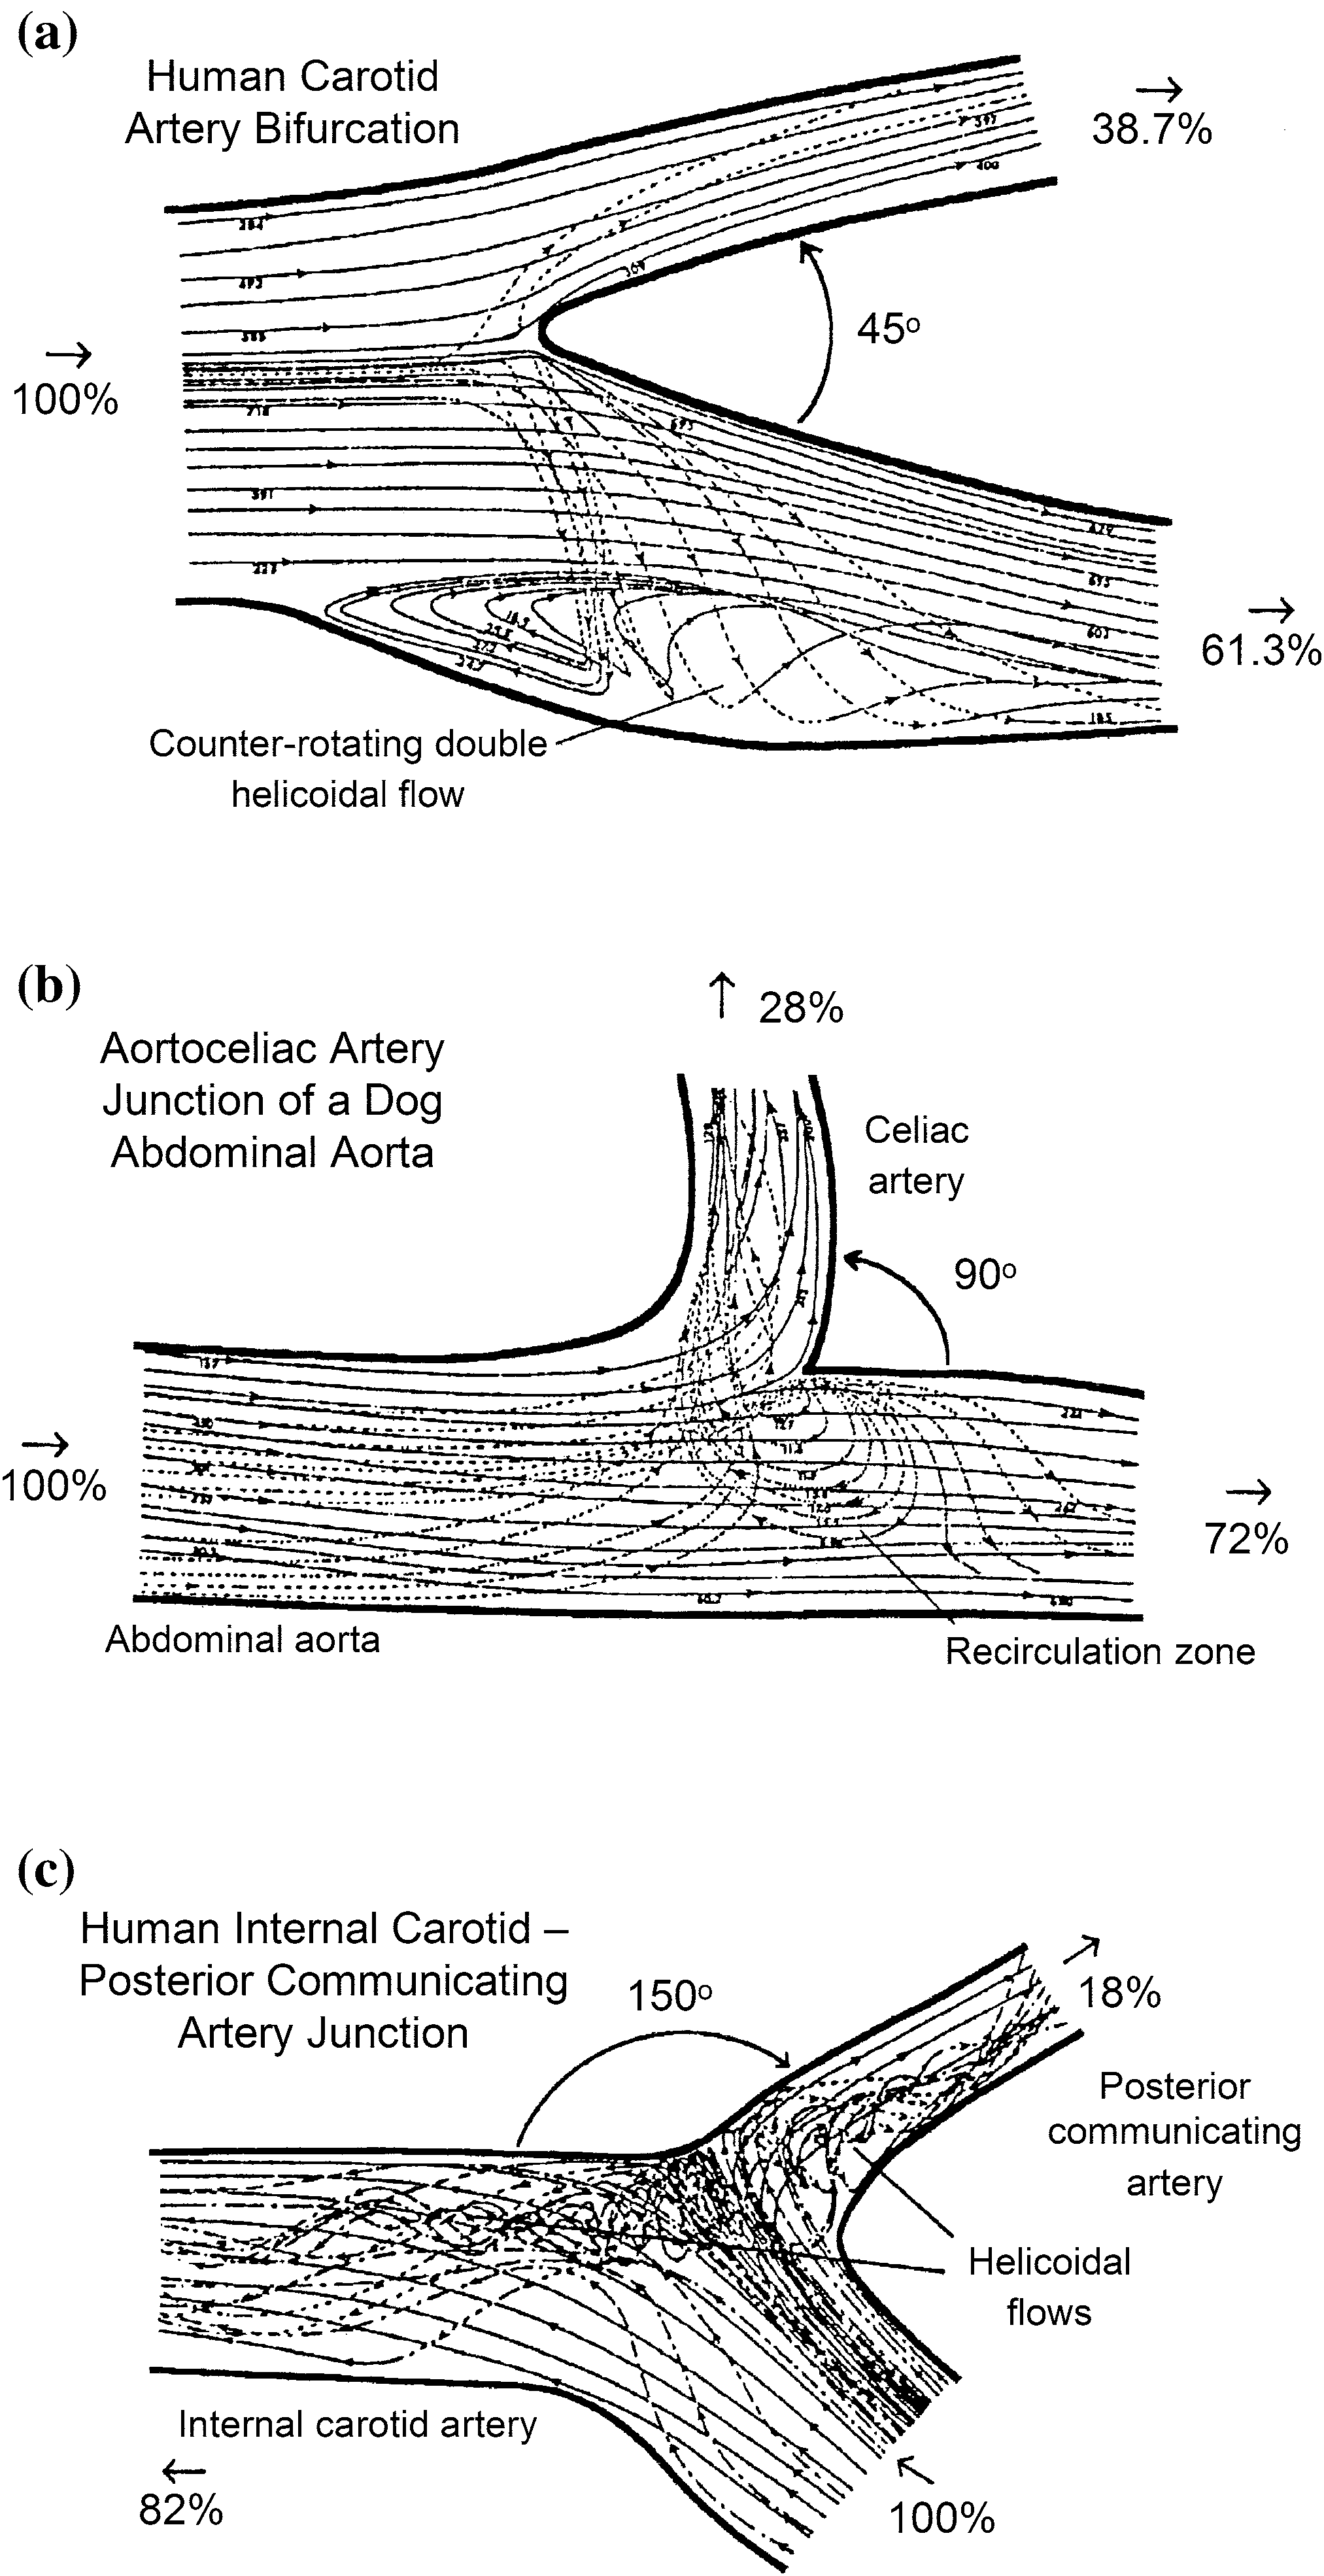
\includegraphics[width=0.4\textwidth]{847.png}
  \caption{Líneas de corriente del flujo perturbado para bifurcaciones a ángulos progresivamente mayores en bifurcaciones, y aproximación al flujo estacionario posterior (De [21], basado en a) [54], b) [38] y c) [39]. Cortesía de Robert A. Freitas Jr., Nanomedicine, Vol.~1 (1999), http://www.nanomedicine.com).}
  \label{fig:847}
\end{figure}



¿Qué tan grande es la fuerza sobre la pared arterial en el vértice? La cantidad de movimiento lineal por unidad de volumen de sangre en la arteria madre (la cual diremos que está en la dirección $x$) es $\rho u_1$, donde $\rho$ es la densidad de masa de la sangre. La cantidad de movimiento por unidad de volumen transportada en cada arteria hija es $\rho u_2$, de la cual $\rho u_2 \cos\theta$ está a lo largo de la dirección $x$. Este cambio en la cantidad de movimiento causa una fuerza sobre la pared arterial. La fuerza que este flujo ejerce sobre una pantalla imaginaria a través del vaso en la arteria madre es el cambio de esta cantidad de movimiento por unidad de tiempo, lo cual es igual a esta cantidad de movimiento lineal por unidad de volumen multiplicada por el caudal:
\begin{equation}
F_{z,\text{parent}} = \rho u_1 Q.
\label{eq:837}
\end{equation}
Debido a que el caudal en cada vaso es $Q/2$ y hay dos de ellos, la fuerza del flujo en las arterias hijas es
\begin{equation}
F_{z,\text{daughters}} = 2 \rho u_2 \cos\theta \frac{Q}{2} = \rho u_2 \cos\theta Q.
\label{eq:838}
\end{equation}
La diferencia de estas fuerzas es
\begin{equation}
F_{\text{arterial wall}} = F_{z,\text{daughters}} - F_{z,\text{parent}} = \rho u_2 \cos\theta Q - \rho u_1 Q = \rho Q (u_2 \cos\theta - u_1)
\label{eq:839}
\end{equation}
o con (8.36)
\begin{equation}
F_{\text{arterial wall}} = \rho Q u_1 \left( \frac{A_1}{2 A_2} \cos\theta - 1 \right) = \rho A_1 u_1^2 \left( \frac{A_1}{2 A_2} \cos\theta - 1 \right).
\label{eq:840}
\end{equation}
Esto tiene un valor negativo máximo de $-\rho Q u_1 = -\rho A_1 u_1^2$ cuando $\theta = 90^\circ$ (el cual es un poco mayor que los ángulos máximos típicos). Debido a que la presión es fuerza/área, si esta fuerza se ejerce sobre la pared del vaso de área de sección transversal $A_1$, como en la Fig.~8.41, existe una presión sobre la pared arterial de
\begin{equation}
P_{\text{arterial wall}} = \frac{\rho Q u_1}{A_1} = \frac{\rho A_1 u_1^2}{A_1} = \rho u_1^2
\label{eq:841}
\end{equation}
(la cual es también la energía cinética por unidad de volumen). Esto puede conducir a la formación de un aneurisma allí. Este mecanismo de cambio de cantidad de movimiento es el mismo que causa una fuerza sobre la pared arterial durante el flujo en una arteria curva. El aneurisma sacular se hace cada vez más grande hasta que se rompe.

El esfuerzo de corte cerca del vértice de la bifurcación debido a la viscosidad es otro factor en la formación de un aneurisma sacular. La Figura~8.46 muestra que en flujo estacionario la velocidad es pequeña cerca de las paredes, y el gradiente de velocidad y consecuentemente el esfuerzo de corte es grande cerca de ellas. Después de la bifurcación y de la transferencia de cantidad de movimiento al vértice, la velocidad de la sangre, el gradiente de velocidad y el corte son mayores cerca de las paredes del vaso después del vértice. El esfuerzo de corte es grande, hasta que el patrón de flujo se reorganiza para dar (7.40) (Fig.~7.11). Esto también se observa en la Fig.~8.47 para bifurcaciones a ángulos cada vez mayores. La ecuación (7.54) se puede utilizar para estimar la distancia desde el vértice para el flujo en estado estacionario. Tenga en cuenta que la ley de Laplace para esferas se aplica a los aneurismas saculares.

\subsection{Ecuación de movimiento de arterias y aneurismas durante el flujo pulsátil (Tema avanzado)}

Para un flujo estacionario, la tensión en la pared arterial equilibra la diferencia de presión dentro y fuera de la arteria, como lo describe la ley de Laplace. Debido a que la presión dentro de la arteria varía realmente dentro de cada ciclo (durante el pulso arterial), este equilibrio debe evaluarse para dar cuenta de estas variaciones cíclicas de presión. Modelemos un aneurisma sacular como una esfera de radio $R$, con una pared delgada de espesor $w$. (De manera similar podríamos modelar un aneurisma fusiforme como un cilindro de radio $R$).

Si el cambio de radio debido a esta presión que varía con el tiempo es $r$, entonces la circunferencia de la esfera cambia de $2\pi R$ a $2\pi(R + r)$. La deformación circunferencial $\epsilon$ es $(2\pi(R + r) - 2\pi R)/2\pi R = r/R$, y el esfuerzo circunferencial $\sigma$ se relaciona con esta deformación mediante
\begin{equation}
\sigma = Y \epsilon = Y \frac{r(t)}{R}.
\label{eq:842}
\end{equation}

La respuesta de la pared arterial tiene una componente que equilibra la presión promedio $P_{\text{av}}$ ---la cual es un promedio ponderado en el tiempo de las presiones sistólica y diastólica para arterias grandes--- y una componente que varía con el tiempo ---debido al pulso $P_{\text{pulse}}(t) = P_{\text{p}} \cos\omega_{\text{p}} t$, donde $P_{\text{p}}$ es una diferencia ponderada en el tiempo de las presiones sistólica y diastólica para arterias grandes y $\omega_{\text{p}}$ es la frecuencia (angular) del pulso---. Esta presión que varía con el tiempo es $P(t) = P_{\text{ss}} + P_{\text{p}} \cos\omega_{\text{p}} t$.

La fuerza de respuesta inercial por unidad de área sobre la esfera es la masa por unidad de área de la cubierta esférica, $\rho w$ ---donde $\rho$ es la densidad de masa---, multiplicada por la aceleración radial, $\mathrm{d}^2 r/\mathrm{d}t^2$, o $\rho w \mathrm{d}^2 r/\mathrm{d}t^2$. El término de presión hidrostática $P(t)$ tiende a aumentar el radio, mientras que el esfuerzo debido a la pared se opone a este cambio, por lo que la respuesta inercial es
\begin{equation}
\rho w \frac{\mathrm{d}^2 r_{\text{p}}(t)}{\mathrm{d}t^2} = P_{\text{av}} + P_{\text{p}} \cos\omega_{\text{p}} t - \frac{Y r(t)}{R}
\label{eq:843}
\end{equation}
debido a que $\mathrm{d}^2 r_{\text{av}}/\mathrm{d}t^2 = 0$.

La perturbación $r(t)$ tiene una componente en respuesta a la presión promedio $P_{\text{av}}$ y una parte que varía con el tiempo en respuesta a la presión del pulso $P_{\text{p}} \cos\omega_{\text{p}} t$. Al sustituir $r(t) = r_{\text{av}} + r_{\text{p}}(t)$ en (8.43), obtenemos
\begin{equation}
\rho w \frac{\mathrm{d}^2 r_{\text{p}}(t)}{\mathrm{d}t^2} = P_{\text{av}} + P_{\text{p}} \cos\omega_{\text{p}} t - \frac{Y [r_{\text{av}} + r_{\text{p}}(t)]}{R}.
\label{eq:844}
\end{equation}

Al igualar los términos que varían con el tiempo para obtener una ecuación y los términos promedio para obtener otra, se llega a
\begin{equation}
\rho w \frac{\mathrm{d}^2 r_{\text{p}}(t)}{\mathrm{d}t^2} = P_{\text{p}} \cos\omega_{\text{p}} t - \frac{Y r_{\text{p}}(t)}{R}
\label{eq:845}
\end{equation}
y
\begin{equation}
0 = P_{\text{av}} - \frac{Y r_{\text{av}}}{R}.
\label{eq:846}
\end{equation}

La ecuación (8.46) está relacionada con la ley de Laplace para una esfera (7.9) ($\Delta P = 2T/R$). La ecuación (8.45) se puede reescribir como
\begin{equation}
\frac{\mathrm{d}^2 r_{\text{p}}(t)}{\mathrm{d}t^2} + \omega_0^2 r_{\text{p}}(t) = \frac{P_{\text{p}}}{\rho w} \cos\omega_{\text{p}} t,
\label{eq:847}
\end{equation}
donde $\omega_0^2 = Y/R\rho w$. Esto se parece a la ecuación de movimiento para un oscilador armónico simple de frecuencia $\omega_0$ más un término adicional (el último), el cual se debe a la fuerza impulsora del pulso a frecuencia $\omega_{\text{p}}$. La solución en estado estacionario para esta ecuación es
\begin{equation}
r_{\text{p}}(t) = \frac{P_{\text{p}} / \rho w}{\omega_0^2 - \omega_{\text{p}}^2} \cos(\omega_{\text{p}} t),
\label{eq:848}
\end{equation}
la cual puede verificarse por sustitución (véase el Apéndice~C). Si $r_{\text{p}}$ es grande, podría conducir a la ruptura. En principio, $r_{\text{p}}$ puede hacerse mayor a medida que el aneurisma se desarrolla porque $Y$, $R$, $\rho$ o $w$ cambian (en $\omega_0^2 = Y/R\rho w$). Sin el término impulsor ($P_{\text{p}} = 0$), la solución es la solución armónica habitual: $r_{\text{p}}(t) = A \cos(\omega_0 t + \phi)$.

Si $\omega_0$ se aproximara a $\omega_{\text{p}}$, (8.48) indica que el cambio de radio se volvería muy grande debido a esta resonancia. Si esto ocurriera (y ocurre en algunos ejemplos de osciladores impulsados, pero en realidad no ocurre para los aneurismas), las propiedades viscosas (o de amortiguamiento) de la pared del vaso tendrían que incluirse a través de un término $\gamma \mathrm{d}r_{\text{p}}/\mathrm{d}t$, lo que conduce a la nueva ecuación de movimiento
\begin{equation}
\frac{\mathrm{d}^2 r_{\text{p}}(t)}{\mathrm{d}t^2} + \gamma \frac{\mathrm{d} r_{\text{p}}(t)}{\mathrm{d}t} + \omega_0^2 r_{\text{p}}(t) = \frac{P_{\text{p}}}{\rho w} \cos\omega_{\text{p}} t
\label{eq:849}
\end{equation}
con la solución en estado estacionario
\begin{equation}
r_{\text{p}}(t) = \frac{(\omega_0^2 - \omega_{\text{p}}^2) P_{\text{p}}/\rho w}{(\omega_0^2 - \omega_{\text{p}}^2)^2 + (\gamma \omega_{\text{p}})^2} \cos(\omega_{\text{p}} t).
\label{eq:850}
\end{equation}

(Véase el Apéndice~C). Esto incluye ahora las propiedades viscoelásticas de la pared arterial, lo cual amortigua un poco la resonancia.

Muy por encima de la resonancia $\omega_0 \simeq \omega_{\text{p}}$ (con $\omega_0 \gg \omega_{\text{p}}$), (8.48) y (8.50) dan
\begin{equation}
r_{\text{p}}(t) \simeq \frac{P_{\text{p}}}{\rho w \omega_0^2} \cos(\omega_{\text{p}} t).
\label{eq:851}
\end{equation}
Sin el término impulsor ($P_{\text{p}} = 0$), la solución es la de un oscilador armónico amortiguado:
\begin{equation*}
r_{\text{p}}(t) = A \exp(-\gamma t/2) \cos(\omega_0 t + \phi) \quad \text{para } \omega_0 \gg \gamma.
\end{equation*}
Esta oscilación armónica se amortigua en un tiempo ${\sim}1/\gamma$, el cual corresponde a aproximadamente $\omega_0/(2\pi\gamma)$ ciclos; este último número a menudo se denomina factor de calidad $Q$ del sistema, como se analiza en la discusión sobre resonancias acústicas del Cap.~10 y en los Apéndices~C y D.

\subsection{Accidentes cerebrovasculares isquémicos}

Durante un accidente cerebrovascular isquémico, se produce el cese del flujo sanguíneo en las arterias que transportan sangre al cerebro debido a una obstrucción o taponamiento luminal. (Como se mencionó anteriormente, la luz ---o lumen--- es la abertura de un vaso sanguíneo). Alrededor del $80\%$ de todos los accidentes cerebrovasculares son isquémicos. Un émbolo es un coágulo de sangre, burbuja de aire (gaseoso) o materia particulada que viaja dentro de un vaso sanguíneo y causa la obstrucción del flujo sanguíneo. Por ejemplo, las lesiones ateroscleróticas (en el cerebro y en otras partes del cuerpo) causan una superficie interna irregular del vaso y la agregación de plaquetas sanguíneas debido a la turbulencia, lo que puede producir émbolos que son agregados plaquetarios. Tales émbolos se pueden formar fuera del cerebro, en el corazón, los pulmones y la circulación sistémica, y viajan al cerebro hasta que llegan a vasos demasiado pequeños para continuar viajando; esto evita el flujo de sangre a regiones más distales (corriente abajo) en el cerebro. Un trombo es una coagulación de la sangre que puede producir un coágulo de fibrina local; esto también puede causar un accidente cerebrovascular isquémico. (Si el trombo se forma y se desplaza a otro lugar, tal como a un vaso de menor diámetro o a un vaso parcialmente ocluido, es un émbolo).

Los accidentes cerebrovasculares pueden ocurrir por estenosis (estrechamiento o cierre de la luz) u oclusiones (cierres u obstrucciones) (Fig.~8.48). Se deben más comúnmente a lesiones ateroscleróticas. Dichas lesiones son masas distribuidas irregularmente de depósitos grasos calcificados que estrechan la luz arterial. Si el diámetro interno normal del vaso es $d_{\text{norm}}$ y el diámetro mínimo debido a la lesión estenótica es $d_{\text{sten}}$, entonces el $\%$ de estenosis se define como: $((d_{\text{norm}} - d_{\text{sten}})/d_{\text{norm}}) \times 100\%$. Se caracterizan por ser leves ($1\text{--}39\%$), moderados ($40\text{--}59\%$), graves ($60\text{--}79\%$), críticos ($80\text{--}99\%$) y ocluidos ($100\%$). La ley de Poiseuille (7.24) muestra que el flujo disminuye a medida que disminuye el diámetro de la luz para una presión inicial dada. El flujo disminuye drásticamente por encima del inicio de la estenosis crítica, y la caída de presión a través de la estenosis aumenta, lo que resulta en la necesidad de una

\begin{SCfigure}[0.9][htbp]
  \centering
  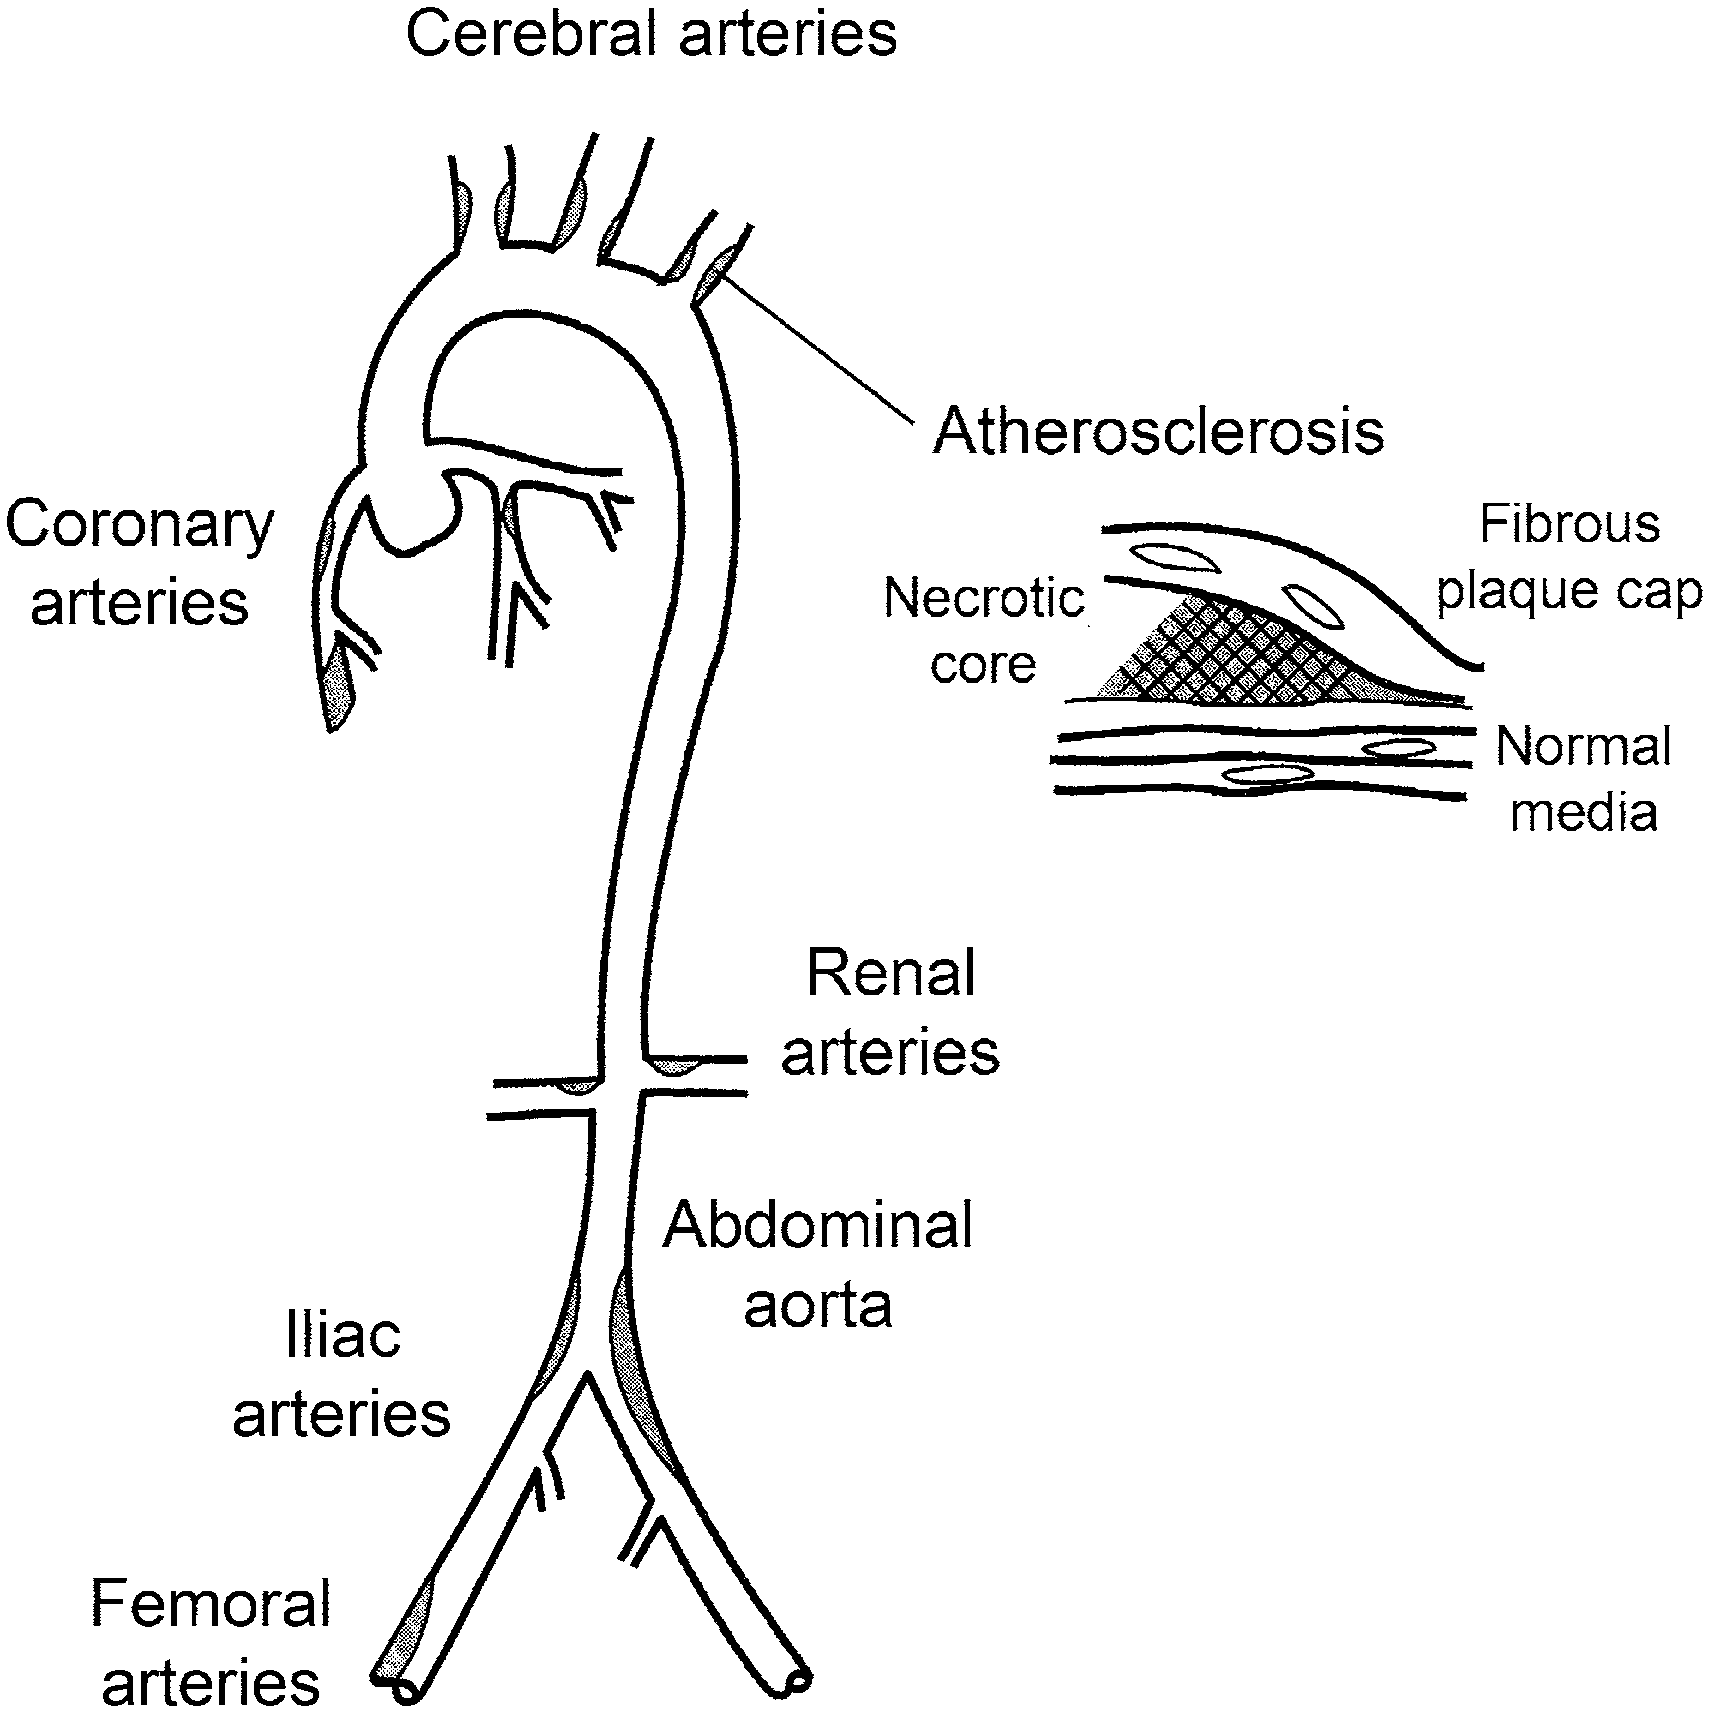
\includegraphics[width=0.5\textwidth]{848.png}
  \caption{Obstrucción de arterias por placa. Se muestra un esquema de la aterosclerosis, junto con algunos de los sitios predilectos de la aterosclerosis en la vasculatura (vasos sanguíneos) (De [36]).}
  \label{fig:848}
\end{SCfigure}



mayor presión sanguínea para mantener el mismo caudal. La física de las arterias obstruidas se analizó anteriormente en este capítulo (Fig.~8.35).

Esta lesión calcificada vuelve rígido al vaso y cambia abruptamente el patrón de flujo a medida que la sangre fluye desde una región elástica y distensible de un vaso hacia esta región rígida y más estrecha, y de regreso a un vaso distensible. El flujo sanguíneo general es más lento debido a la estenosis (a menos que la presión aumente), lo que puede provocar la coagulación. El coágulo resultante (o trombo) no se adhiere bien a la pared del vaso y puede desplazarse a otra parte de la corriente de flujo, y este émbolo puede provocar un accidente cerebrovascular. Dentro de la estenosis misma, el flujo sanguíneo es más rápido que justo antes de ella, según el principio de Bernoulli. Este aumento del flujo sanguíneo tiene varias consecuencias negativas. A medida que esta energía cinética incrementada (por unidad de volumen) en la región estenótica disminuye en el vaso normal postestenótico (debido al principio de Bernoulli), puede producirse fatiga estructural en esta última región, lo que provoca distensión, y esta posible dilatación puede conducir a un aneurisma fusiforme. El aumento de la velocidad del flujo estenótico y la geometría irregular pueden incrementar el número de Reynolds, lo que resulta en un flujo turbulento y el eventual desprendimiento de la placa arterial, que luego se convierte en un émbolo particulado. El aumento de la velocidad también conduce a mayores esfuerzos cortantes sobre la lesión.

\section{Modelado del sistema circulatorio y del corazón}

La ramificación en el sistema circulatorio es muy compleja. Aun así, existe una transición ordenada de arterias más grandes a más pequeñas y luego de venas más pequeñas a más grandes, por lo que podemos imaginar un modelo general de la circulación en el que todas las arterias o venas de un diámetro dado se combinan para formar un subsistema. Hemos visto que los vasos más grandes se pueden modelar bastante bien como vasos de compliancia ideales, mientras que los vasos más pequeños se pueden modelar como vasos de resistencia. Ahora utilizaremos estos modelos para desarrollar un modelo integral de la circulación, que pueda manejar tanto el flujo en estado estacionario como los cambios que dependen del tiempo, como el pulso arterial. Este modelo se puede utilizar para comprender el control de la circulación.

Para un modelo de circulación completo, necesitamos incluir la acción del corazón, que en realidad consiste en dos bombas separadas: el corazón derecho para el sistema pulmonar y el corazón izquierdo para el sistema sistémico. Primero desarrollamos modelos estáticos y dinámicos de los corazones izquierdo y derecho.

\subsection{Modelo del corazón}

Consideremos el ventrículo izquierdo, que es la bomba principal del corazón izquierdo; el tratamiento del corazón derecho es análogo. Durante la sístole, la válvula mitral está cerrada y la válvula aórtica está abierta. La presión que se desarrolla es esencialmente la de las arterias sistémicas (sa), $P_{\text{sa}}$, debido a la caída de presión extremadamente pequeña. Durante la diástole, la válvula aórtica está cerrada y la válvula mitral está abierta. El ventrículo izquierdo recibe sangre de la aurícula izquierda a una presión bastante baja, que es esencialmente igual a la de las venas pulmonares (pv), $P_{\text{pv}} \sim 5\text{ mmHg}$, que alimenta la aurícula izquierda.

\subsubsection*{Modelo estático de los ventrículos}

Modelaremos el ventrículo izquierdo (o derecho) como una cubierta hemisférica, con un radio interno $r_{\text{i}}$ y un radio externo $r_{\text{o}}$, con una pared muy gruesa de espesor $r_{\text{o}} - r_{\text{i}}$. Asumamos que el lado abierto está orientado hacia arriba, como en la Fig.~8.49. La presión (manométrica) interna $P_{\text{i}}$ empuja el ventrículo hacia abajo y alcanza un máximo durante la sístole de $120\text{ mmHg}$. La presión externa (que actúa sobre la superficie inferior redondeada) $P_{\text{o}}$ proviene del pericardio y empuja el ventrículo hacia arriba, y es aproximadamente la presión pleural, la cual puede ser negativa (es decir, menor que una atmósfera). El esfuerzo de pared circunferencial $\sigma$ actúa verticalmente y empuja el ventrículo hacia arriba. Estos argumentos son los mismos que los de la ley de Laplace para una esfera (7.9), excepto que ahora asumimos que la pared tiene un espesor finito.

\begin{SCfigure}[0.9][htbp]
  \centering
  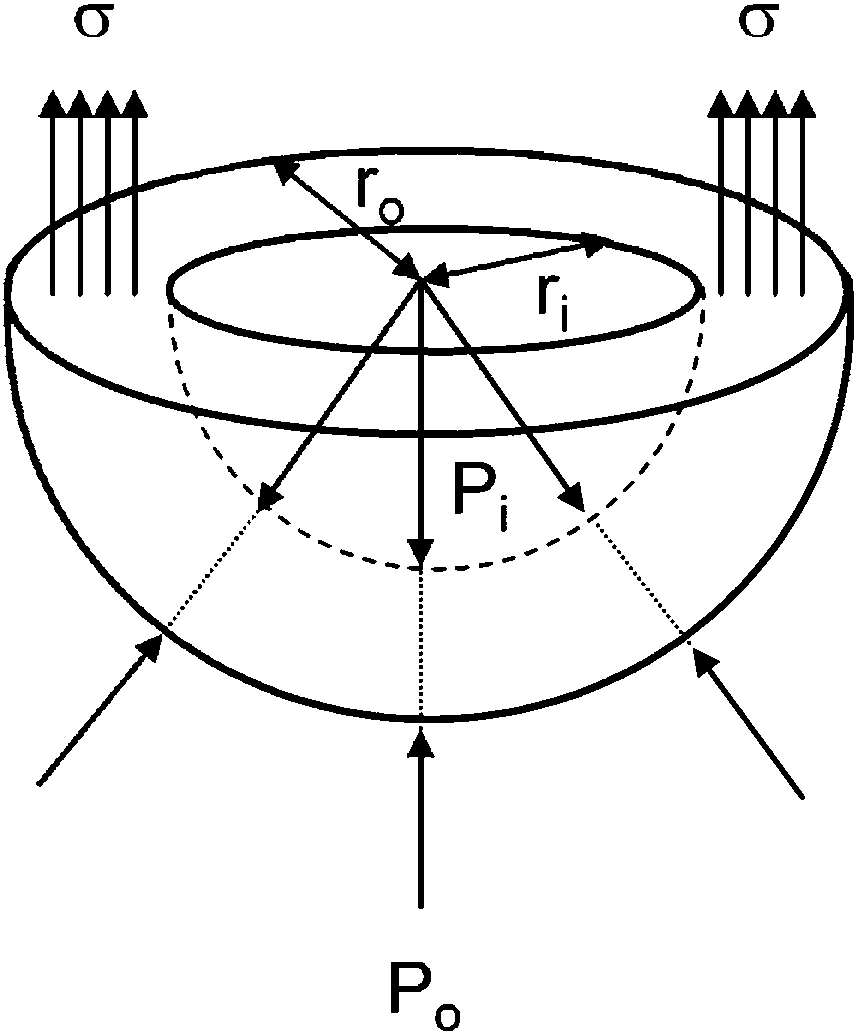
\includegraphics[width=0.5\textwidth]{849.png}
  \caption{Modelo del ventrículo izquierdo (Basado en [50]).}
  \label{fig:849}
\end{SCfigure}



El equilibrio de fuerzas en la dirección vertical da
\begin{equation}
(\pi r_{\text{i}}^2) P_{\text{i}} = (\pi r_{\text{o}}^2) P_{\text{o}} + \left( \pi (r_{\text{o}}^2 - r_{\text{i}}^2) \right) \sigma,
\label{eq:852}
\end{equation}
y, por lo tanto, el esfuerzo de pared circunferencial es
\begin{equation}
\sigma = \frac{P_{\text{i}} r_{\text{i}}^2 - P_{\text{o}} r_{\text{o}}^2}{r_{\text{o}}^2 - r_{\text{i}}^2}.
\label{eq:853}
\end{equation}

Los dos primeros términos en (\ref{eq:852}) no son simplemente las áreas superficiales de las áreas respectivas, $2\pi r_{\text{i,o}}^2$, multiplicadas por la presión hidrostática, $P_{\text{i,o}}$, sino la mitad de eso, debido a que solo una parte de la fuerza debida a la presión actúa en la dirección vertical (como en la ley de Laplace para esferas y en el Problema~7.12). Dado que $P_{\text{i}} \gg P_{\text{o}}$,
\begin{equation}
\sigma \simeq \frac{P_{\text{i}}}{(r_{\text{o}}/r_{\text{i}})^2 - 1}.
\label{eq:854}
\end{equation}

Debido a que el material en la pared del corazón es incompresible, el volumen de la pared del corazón, $V_{\text{wall}}$, no cambia con la presión. A partir de la diferencia de los volúmenes de las cubiertas hemisféricas externa e interna, sabemos que $V_{\text{wall}} = 2\pi (r_{\text{o}}^3 - r_{\text{i}}^3)/3$ y, por lo tanto, $(r_{\text{o}}/r_{\text{i}})^2 = (1 + V_{\text{wall}}/V_{\text{i}})^{2/3}$, donde el volumen interno del ventrículo izquierdo es $V_{\text{i}} = 2\pi r_{\text{i}}^3/3$. Por lo tanto, vemos que
\begin{equation}
\sigma \simeq \frac{P_{\text{i}}}{(1 + V_{\text{wall}}/V_{\text{i}})^{2/3} - 1}.
\label{eq:855}
\end{equation}

Utilizando la expansión $(1 + x)^n \simeq 1 + nx$ para $|x| \ll 1$ y el hecho de que el volumen interno del ventrículo izquierdo es mucho mayor que el volumen de la pared del corazón, encontramos
\begin{equation}
\sigma \simeq \frac{3 V_{\text{i}}}{2 V_{\text{wall}}} P_{\text{i}}.
\label{eq:856}
\end{equation}

Esto muestra cómo una presión sistólica excesiva o el agrandamiento del ventrículo izquierdo (y del corazón) conducirá a un esfuerzo excesivo en la pared cardíaca (para un espesor de pared constante).

\subsubsection*{Modelo dinámico de los ventrículos}

Ahora modelaremos un ventrículo como un vaso de compliancia con una compliancia que varía con el tiempo \cite{34}, de modo que utilizamos (8.5)
\begin{equation}
V(t) = V_{\text{d}} + C(t) P(t).
\label{eq:857}
\end{equation}
(En esta sección llamaremos simplemente $R$ y $C$ a la resistencia al flujo $R_{\text{flow}}$ y a la compliancia $C_{\text{flow}}$, respectivamente). La Fig.~8.50 muestra cómo cambia la compliancia del ventrículo durante un ciclo cardíaco. Tenga en cuenta que en este gráfico y en otros relacionados, una mayor compliancia corresponde a una pendiente menor debido a que $P$ se grafica como una función de $V$. Durante la sístole, la compliancia se vuelve baja, lo que hace que se desarrolle una presión alta debido a que el volumen permanece bastante constante. En la diástole, el ventrículo se relaja, lo cual está asociado con una compliancia grande que induce una presión baja.

\begin{SCfigure}[0.8][htbp]
  \centering
  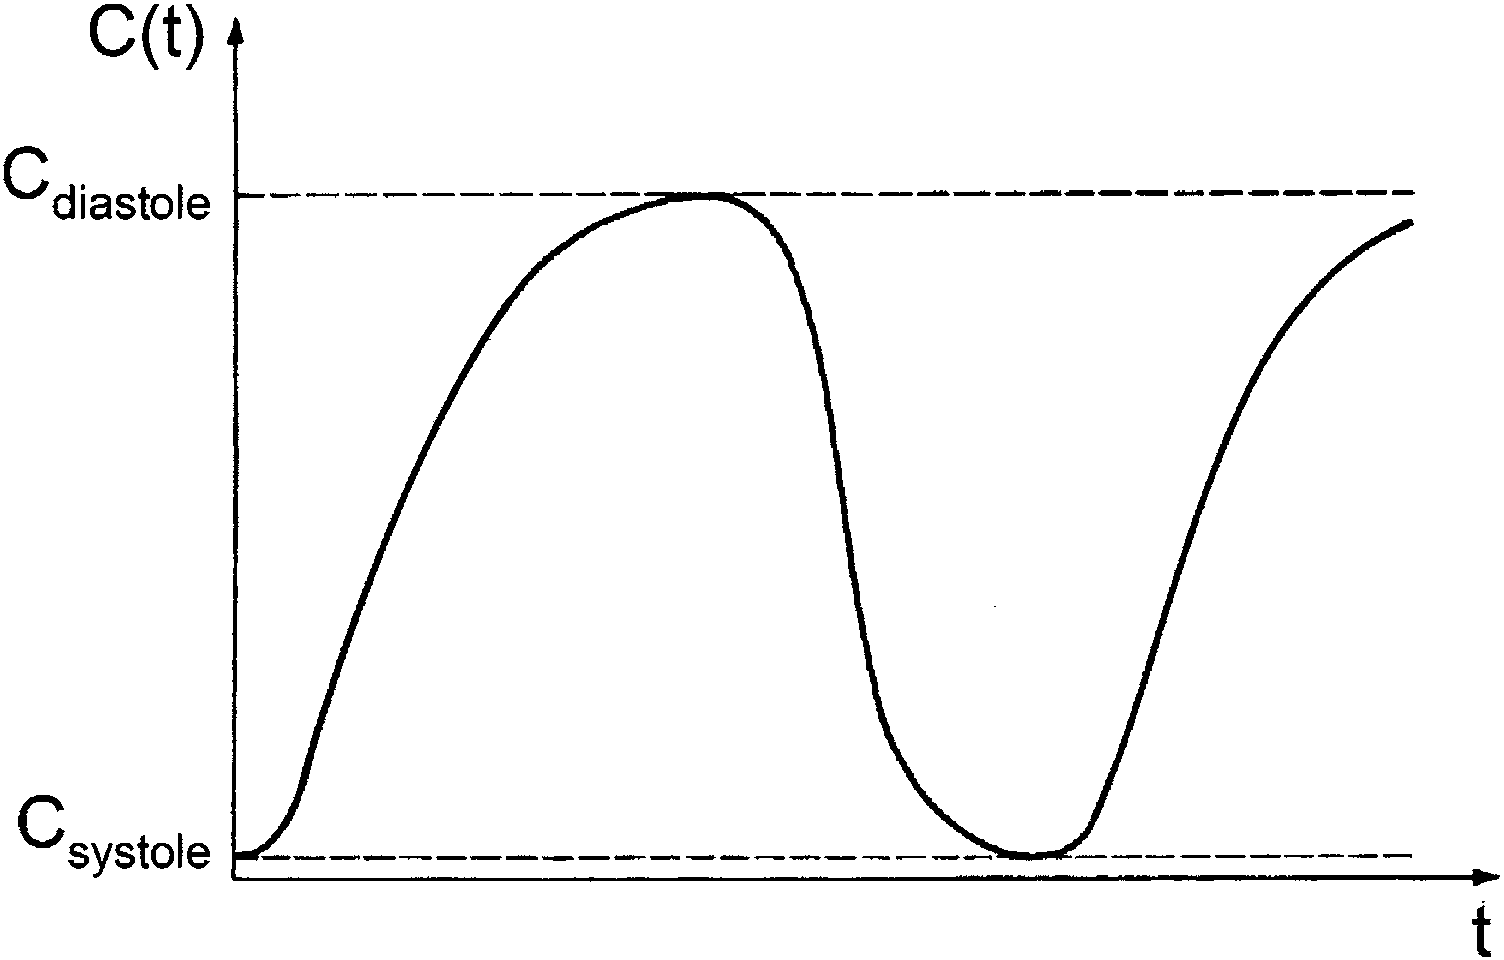
\includegraphics[width=0.55\textwidth]{850.png}
  \caption{Cambios en la compliancia del ventrículo durante el ciclo cardíaco, desde un valor pequeño mientras se contrae durante la sístole hasta un valor grande al relajarse durante la diástole (De [34]).}
  \label{fig:850}
\end{SCfigure}



Los cambios de volumen y presión en el ventrículo durante un ciclo cardíaco se modelan en la Fig.~8.51. La etapa A ocurre cuando la válvula de entrada (que es la válvula mitral para el VI) se cierra, lo que marca el final de la diástole (ED) y el comienzo de la sístole. El volumen del ventrículo es máximo, con
\begin{equation}
V_{\text{ED}} = V_{\text{d}} + C_{\text{diastole}} P_{\text{pv}}
\label{eq:858}
\end{equation}
para el ventrículo izquierdo. Durante la sístole, la compliancia disminuye isovolumétricamente, por lo que la presión aumenta. En la etapa B, la válvula de salida (que es la válvula aórtica para el VI) se abre; la presión permanece constante a medida que la sangre sale del ventrículo y, de forma concomitante, el volumen del ventrículo disminuye. La etapa C ocurre cuando la válvula de salida se cierra, lo que marca el final de la sístole (ES) y el comienzo de la diástole. El volumen del ventrículo es mínimo, con
\begin{equation}
V_{\text{ES}} = V_{\text{d}} + C_{\text{systole}} P_{\text{sa}}
\label{eq:859}
\end{equation}
para el ventrículo izquierdo. Durante la diástole, la compliancia aumenta isovolumétricamente, por lo que la presión disminuye. En la etapa D, la válvula de entrada se abre; la presión permanece entonces constante a medida que la sangre ingresa al ventrículo y, de forma concomitante, el volumen del ventrículo aumenta, hasta que se alcanza nuevamente el final de la diástole, la etapa A.

El volumen sistólico es
\begin{equation}
V_{\text{stroke}} = V_{\text{ED}} - V_{\text{ES}} = C_{\text{diastole}} P_{\text{pv}} - C_{\text{systole}} P_{\text{sa}}
\label{eq:860}
\end{equation}
para el ventrículo izquierdo. Debido a que $C_{\text{systole}} \sim 0$, podemos tomar
\begin{equation}
V_{\text{stroke}} = C_{\text{diastole}} P_{\text{pv}}.
\label{eq:861}
\end{equation}

Con una frecuencia cardíaca $F$, el caudal volumétrico es
\begin{equation}
Q = F V_{\text{stroke}} = F C_{\text{diastole}} P_{\text{pv}}.
\label{eq:862}
\end{equation}
Llamando $K = F C_{\text{diastole}}$ al coeficiente de la bomba, podemos modelar el ventrículo izquierdo mediante
\begin{equation}
Q_{\text{L}} = K_{\text{L}} P_{\text{pv}}.
\label{eq:863}
\end{equation}
De manera análoga para el corazón derecho, el ventrículo derecho, que se alimenta de las venas sistémicas (sv), se modela mediante
\begin{equation}
Q_{\text{R}} = K_{\text{R}} P_{\text{sv}}.
\label{eq:864}
\end{equation}

\subsection{Modelo del flujo general en el sistema circulatorio}

Modelaremos los ocho subsistemas que se muestran en la Fig.~8.52: dos corazones (L y R), arterias grandes en los sistemas sistémico y pulmonar (sa y pa), venas grandes en los sistemas sistémico y pulmonar (sv y pv), y los vasos pequeños (arteriolas/capilares/vénulas) en los sistemas sistémico y pulmonar \cite{34, 40, 59}. La sangre fluye desde el ventrículo izquierdo sucesivamente a través de las arterias grandes sistémicas, los vasos pequeños y las venas grandes, y hacia el ventrículo derecho. Luego, la sangre va desde el ventrículo derecho sucesivamente a través de las arterias grandes pulmonares, los vasos pequeños y las venas grandes, y hacia el ventrículo izquierdo.

\begin{SCfigure}[0.9][htbp]
  \centering
  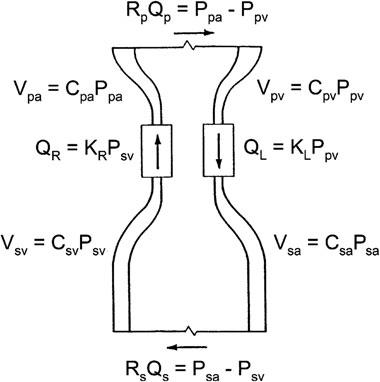
\includegraphics[width=0.5\textwidth]{852.png}
  \caption{Los ocho subsistemas en el flujo sistémico y pulmonar, con sus ecuaciones de modelo (De [34]).}
  \label{fig:852}
\end{SCfigure}



Los flujos a través de los ventrículos están determinados por las presiones en las venas que los alimentan (a través de las aurículas)
\begin{equation}
Q_{\text{L}} = K_{\text{L}} P_{\text{pv}} \quad \text{y} \quad Q_{\text{R}} = K_{\text{R}} P_{\text{sv}}.
\label{eq:865}
\end{equation}
Los volúmenes en las arterias grandes están determinados por sus compliancias y las presiones dentro de ellas
\begin{equation}
V_{\text{sa}} = C_{\text{sa}} P_{\text{sa}} \quad \text{y} \quad V_{\text{pa}} = C_{\text{pa}} P_{\text{pa}},
\label{eq:866}
\end{equation}
al igual que los volúmenes de las venas
\begin{equation}
V_{\text{sv}} = C_{\text{sv}} P_{\text{sv}} \quad \text{y} \quad V_{\text{pv}} = C_{\text{pv}} P_{\text{pv}}.
\label{eq:867}
\end{equation}

(Un modelo más refinado incluiría el volumen muerto en estos vasos grandes). La caída de presión a través de los vasos pequeños es la diferencia de presión entre las arterias grandes y las venas grandes. Para los sistemas sistémico y pulmonar respectivos, la caída de presión está determinada por sus resistencias ($R_{\text{s}}$ y $R_{\text{p}}$) y los flujos a través de ellos ($Q_{\text{s}}$ y $Q_{\text{p}}$)
\begin{equation}
P_{\text{sa}} - P_{\text{sv}} = R_{\text{s}} Q_{\text{s}} \quad \text{y} \quad P_{\text{pa}} - P_{\text{pv}} = R_{\text{p}} Q_{\text{p}}.
\label{eq:868}
\end{equation}

Vemos una simetría aquí. Hay tres tipos de variables: el flujo $Q$, el volumen $V$ y la presión $P$. Cada subsistema depende de las relaciones entre dos de ellas: $Q$ y $P$ para los ventrículos, $V$ y $P$ para los vasos grandes, y $P$ y $Q$ para los vasos pequeños.

Hay 12 incógnitas: cuatro flujos: $Q_{\text{R}}$, $Q_{\text{L}}$, $Q_{\text{s}}$, $Q_{\text{p}}$; cuatro presiones: $P_{\text{sa}}$, $P_{\text{sv}}$, $P_{\text{pa}}$, $P_{\text{pv}}$; y cuatro volúmenes: $V_{\text{sa}}$, $V_{\text{sv}}$, $V_{\text{pa}}$, $V_{\text{pv}}$. Necesitamos 12 ecuaciones para resolver estas 12 incógnitas, pero aquí solo tenemos ocho y necesitamos cuatro más. Sin embargo, para un flujo en estado estacionario, el flujo en cada región es el mismo, por lo que $Q_{\text{R}} = Q_{\text{L}} = Q_{\text{s}} = Q_{\text{p}}$. Estas son en realidad las tres ecuaciones independientes
\begin{equation}
Q_{\text{R}} = Q_{\text{L}}, \quad Q_{\text{L}} = Q_{\text{s}} \quad \text{y} \quad Q_{\text{R}} = Q_{\text{p}},
\label{eq:869}
\end{equation}
donde cada caudal es igual a $Q$. La cuarta ecuación describe el volumen total constante y es
\begin{equation}
V_0 = V_{\text{sa}} + V_{\text{sv}} + V_{\text{pa}} + V_{\text{pv}}.
\label{eq:870}
\end{equation}

Ahora podemos resolver estas ecuaciones. A partir de las ecuaciones de la bomba (\ref{eq:863}) y (\ref{eq:864}), las presiones venosas son
\begin{equation}
P_{\text{sv}} = \frac{Q}{K_{\text{R}}} \quad \text{y} \quad P_{\text{pv}} = \frac{Q}{K_{\text{L}}}.
\label{eq:871}
\end{equation}

Insertar estas presiones venosas en las ecuaciones de resistencia (\ref{eq:868}) da
\begin{equation}
P_{\text{sa}} = \frac{Q}{K_{\text{R}}} + R_{\text{s}} Q \quad \text{y} \quad P_{\text{pa}} = \frac{Q}{K_{\text{L}}} + R_{\text{p}} Q.
\label{eq:872}
\end{equation}

Insertar estas presiones venosas y arteriales en las ecuaciones de compliancia (\ref{eq:866}) y (\ref{eq:867}) da
\begin{equation}
V_{\text{sa}} = Q C_{\text{sa}} \left( \frac{1}{K_{\text{R}}} + R_{\text{s}} \right) \quad \text{y} \quad V_{\text{pa}} = Q C_{\text{pa}} \left( \frac{1}{K_{\text{L}}} + R_{\text{p}} \right)
\label{eq:873}
\end{equation}
y
\begin{equation}
V_{\text{sv}} = Q C_{\text{sv}} \left( \frac{1}{K_{\text{R}}} \right) \quad \text{y} \quad V_{\text{pv}} = Q C_{\text{pv}} \left( \frac{1}{K_{\text{L}}} \right).
\label{eq:874}
\end{equation}

Estas se pueden expresar como
\begin{equation}
V_{\text{i}} = T_{\text{i}} Q \quad \text{para} \quad i = \text{sv}, \text{pv}, \text{sa}, \text{pa},
\label{eq:875}
\end{equation}
con
\begin{equation}
T_{\text{sa}} = C_{\text{sa}} \left( \frac{1}{K_{\text{R}}} + R_{\text{s}} \right) \quad \text{y} \quad T_{\text{pa}} = C_{\text{pa}} \left( \frac{1}{K_{\text{L}}} + R_{\text{p}} \right)
\label{eq:876}
\end{equation}
y
\begin{equation}
T_{\text{sv}} = C_{\text{sv}} \left( \frac{1}{K_{\text{R}}} \right) \quad \text{y} \quad T_{\text{pv}} = C_{\text{pv}} \left( \frac{1}{K_{\text{L}}} \right).
\label{eq:877}
\end{equation}

Insertar estas ecuaciones en (\ref{eq:870}) para el volumen total de sangre da
\begin{equation}
V_0 = V_{\text{sa}} + V_{\text{sv}} + V_{\text{pa}} + V_{\text{pv}}
\label{eq:878}
\end{equation}
\begin{equation}
= Q(T_{\text{sa}} + T_{\text{sv}} + T_{\text{pa}} + T_{\text{pv}})
\label{eq:879}
\end{equation}
o bien
\begin{equation}
Q = \frac{V_0}{T_{\text{sa}} + T_{\text{sv}} + T_{\text{pa}} + T_{\text{pv}}}.
\label{eq:880}
\end{equation}

Todos los volúmenes se obtienen a partir de esto y de (\ref{eq:875})
\begin{equation}
V_{\text{i}} = \frac{T_{\text{i}} V_0}{T_{\text{sa}} + T_{\text{sv}} + T_{\text{pa}} + T_{\text{pv}}}
\label{eq:881}
\end{equation}
y todas las presiones a partir de $P_{\text{i}} = V_{\text{i}}/C_{\text{i}}$ (de (\ref{eq:866}) y (\ref{eq:867}))
\begin{equation}
P_{\text{i}} = \frac{1}{C_{\text{i}}} \frac{T_{\text{i}} V_0}{T_{\text{sa}} + T_{\text{sv}} + T_{\text{pa}} + T_{\text{pv}}}.
\label{eq:882}
\end{equation}

\begin{table}[htbp]
\centering
\caption{Parámetros normales en reposo del modelo de circulación (Utilizando datos de \cite{34}).}
\label{tab:88}
\begin{tabularx}{\textwidth}{lXX}
\toprule
 & Sistema sistémico & Sistema pulmonar \\
\midrule
Resistencia, $\text{mmHg/(L/min)}$ & $R_{\text{s}} = 17{,}5$ & $R_{\text{p}} = 1{,}79$ \\
Compliancia, $\text{L/mmHg}$ & & \\
\quad Arterial & $C_{\text{sa}} = 0{,}01$ & $C_{\text{pa}} = 0{,}00667$ \\
\quad Venosa & $C_{\text{sv}} = 1{,}75$ & $C_{\text{pv}} = 0{,}08$ \\
Corazón & $K_{\text{L}} = 1{,}12$ & $K_{\text{R}} = 2{,}8$ \\
\midrule
\multicolumn{3}{l}{Volumen total: $V_0 = 5{,}0\text{ L}$} \\
\bottomrule
\end{tabularx}
\end{table}

Con valores conocidos del caudal y del volumen total, se pueden determinar los parámetros del modelo; véase la Tabla~8.8.

Este modelo se puede adaptar a la circulación sanguínea en el feto en desarrollo incluyendo los flujos a través del conducto arterioso (la derivación desde la arteria pulmonar hacia la aorta, representada aquí por las arterias sistémicas), $Q_{\text{d}}$, y del foramen oval (la derivación que permite el flujo desde la aurícula derecha hacia la izquierda, representada aquí por el flujo desde el corazón derecho hacia el izquierdo), $Q_{\text{f}}$ \cite{34, 40}. (En este modelo, el sistema sistémico fetal incluye los vasos que pasan a través del cordón umbilical para conectarse con la placenta). Anteriormente, la continuidad del flujo nos dio $Q_{\text{R}} = Q_{\text{L}} = Q_{\text{s}} = Q_{\text{p}}$, lo que condujo a tres ecuaciones independientes para el flujo (\ref{eq:869}). Todavía existen cuatro ecuaciones de flujo (Problema~8.55):
\begin{equation}
Q_{\text{R}} = Q_{\text{p}} + Q_{\text{d}}
\label{eq:883}
\end{equation}
\begin{equation}
Q_{\text{d}} + Q_{\text{L}} = Q_{\text{s}}
\label{eq:884}
\end{equation}
\begin{equation}
Q_{\text{s}} = Q_{\text{R}} + Q_{\text{f}}
\label{eq:885}
\end{equation}
\begin{equation}
Q_{\text{p}} + Q_{\text{f}} = Q_{\text{L}},
\label{eq:886}
\end{equation}
las cuales corresponden respectivamente a las arterias pulmonares y sistémicas y a las venas sistémicas y pulmonares. Al sumarlas se obtiene una identidad (Problema~8.56), por lo que todavía tenemos únicamente tres ecuaciones de flujo independientes. Debido a que agregamos dos nuevas variables, necesitamos dos nuevas ecuaciones. Estas se obtienen al modelar el conducto arterioso como un vaso de resistencia con una resistencia $R_{\text{d}}$
\begin{equation}
P_{\text{pa}} - P_{\text{sa}} = R_{\text{d}} Q_{\text{d}}
\label{eq:887}
\end{equation}
y el foramen oval como una válvula ideal que está abierta
\begin{equation}
Q_{\text{f}} \ge 0 \quad \text{y} \quad P_{\text{sv}} = P_{\text{pv}}
\label{eq:888}
\end{equation}
(la condición normal para el feto en desarrollo) o cerrada
\begin{equation}
Q_{\text{f}} = 0 \quad \text{y} \quad P_{\text{sv}} \le P_{\text{pv}}
\label{eq:889}
\end{equation}
(la condición normal para el bebé justo después del nacimiento).

Esbozaremos aquí los puntos clave de la solución general y discutiremos el modelo con más detalle en los Problemas 8.54 a 8.59. Las ecuaciones de flujo se pueden reorganizar para obtener
\begin{equation}
Q_{\text{s}} = Q_{\text{L}} + Q_{\text{d}}
\label{eq:890}
\end{equation}
\begin{equation}
Q_{\text{p}} = Q_{\text{R}} - Q_{\text{d}}
\label{eq:891}
\end{equation}
\begin{equation}
Q_{\text{f}} = Q_{\text{L}} - Q_{\text{R}} + Q_{\text{d}}.
\label{eq:892}
\end{equation}

La segunda ecuación muestra que debe haber flujo a través del conducto arterioso para disminuir el flujo en el sistema pulmonar (y en los pulmones). La tercera ecuación muestra que debe haber flujos comparables a través de ambas derivaciones (y, además, que debe haber dos derivaciones y no una), debido a que los corazones izquierdo y derecho en el feto en desarrollo tienen aproximadamente el mismo tamaño y están diseñados para tener aproximadamente los mismos flujos.

Antes del nacimiento podemos (1) asumir que la resistencia pulmonar es muy alta para evitar el flujo de sangre a través de los pulmones fetales (los cuales no están involucrados en la oxigenación de la sangre) y, por lo tanto, $R_{\text{p}} > R_{\text{s}}$ (mientras que después del nacimiento $R_{\text{p}} < R_{\text{s}}$), (2) establecer $K_{\text{R}} = K_{\text{L}} = K$ debido a que los corazones izquierdo y derecho en el feto tienen aproximadamente el mismo tamaño, (3) establecer $R_{\text{d}} = 0$ debido a que el conducto arterioso está completamente abierto y, por lo tanto, $P_{\text{sa}} = P_{\text{pa}} = P_{\text{a}}$, y (4) asumir que el foramen oval está abierto, por lo que $P_{\text{sv}} = P_{\text{pv}} = P_{\text{v}}$. La solución del modelo de circulación fetal con estas suposiciones confirma que $Q_{\text{f}} \ge 0$, por lo que esta suposición y la solución son autoconsistentes.

Justo después del nacimiento y de la primera bocanada de aire, los pulmones del bebé se expanden y entonces $R_{\text{p}} < R_{\text{s}}$, por lo que nuestra suposición (1) deja de ser válida. El Problema~8.57 muestra que entonces nuestra suposición (4) de $Q_{\text{f}} \ge 0$ también deja de ser válida, lo que significa que el foramen oval ahora está cerrado. El modelo se debe resolver nuevamente asumiendo que está cerrado (lo cual se puede verificar en la solución), manteniendo únicamente las suposiciones (2) y (3) (Problema~8.59). Esta solución muestra que, después del nacimiento, el flujo en el conducto arterioso invierte su dirección, fluyendo ahora la sangre desde la aorta (arterias sistémicas) hacia las arterias pulmonares, y que el foramen oval está de hecho cerrado. A medida que el bebé crece, ambas derivaciones permanecen cerradas de forma permanente en los bebés sanos, y el corazón izquierdo crece más rápido que el corazón derecho.

\subsection{El pulso arterial}

Este modelo es capaz de analizar mucho más que simplemente este flujo promedio idealizado. Podemos utilizarlo para comprender el pulso arterial, que es la desviación periódica de la presión arterial sistémica con respecto al valor diastólico debido a la sístole (Fig.~8.53). Esta presión de pulso es
\begin{equation}
P_{\text{pulse}} = P_{\text{systole}} - P_{\text{diastole}},
\label{eq:893}
\end{equation}
la cual es de $\sim 40\text{ mmHg}$ ($= 120\text{ mmHg} - 80\text{ mmHg}$). Estas suposiciones de estado estacionario que hemos venido realizando ya no son apropiadas para este flujo pulsátil.

\begin{SCfigure}[0.75][htbp]
  \centering
  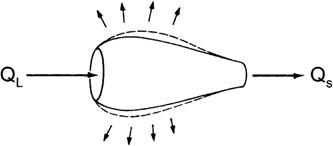
\includegraphics[width=0.6\textwidth]{853.png}
  \caption{El pulso arterial sistémico. Véase también la presión aórtica en la Fig.~8.5 (De [34]).}
  \label{fig:853}
\end{SCfigure}



Considere el sistema de arterias sistémicas, que tiene un volumen $V_{\text{sa}}$ y una presión $P_{\text{sa}}$. Como vaso de compliancia, su volumen puede cambiar, y cambiará cuando el flujo de entrada no sea igual al flujo que sale de él (Fig.~8.54). El flujo que entra es el proveniente del corazón izquierdo, $Q_{\text{L}}$, y el flujo que sale va hacia el sistema de vasos pequeños (no compliantes), el cual tiene un flujo $Q_{\text{s}}$. La conservación del volumen da
\begin{equation}
\frac{\mathrm{d}V_{\text{sa}}(t)}{\mathrm{d}t} = Q_{\text{L}}(t) - Q_{\text{s}}(t).
\label{eq:894}
\end{equation}

\begin{SCfigure}[0.8][htbp]
  \centering
  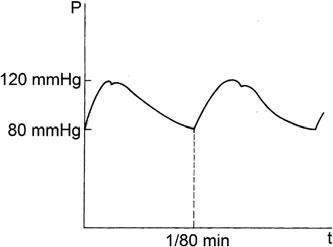
\includegraphics[width=0.55\textwidth]{854.png}
  \caption{Durante el flujo pulsátil, el cambio del volumen arterial es igual al flujo de entrada volumétrico menos el de salida, como lo requiere la conservación del volumen (masa) (De [34]).}
  \label{fig:854}
\end{SCfigure}



Para este vaso de compliancia sabemos que
\begin{equation}
V_{\text{sa}}(t) = V_{\text{sa,d}} + C_{\text{sa}} P_{\text{sa}}(t),
\label{eq:895}
\end{equation}
donde ahora hemos incluido el volumen muerto. Diferenciar esta ecuación con respecto al tiempo y combinarla con la ecuación anterior da
\begin{equation}
\frac{\mathrm{d}V_{\text{sa}}(t)}{\mathrm{d}t} = C_{\text{sa}} \frac{\mathrm{d}P_{\text{sa}}(t)}{\mathrm{d}t} = Q_{\text{L}}(t) - Q_{\text{s}}(t).
\label{eq:896}
\end{equation}

Utilizar (\ref{eq:868}) da
\begin{equation}
R_{\text{s}} Q_{\text{s}} = P_{\text{sa}} - P_{\text{sv}} \sim P_{\text{sa}}
\label{eq:897}
\end{equation}
dado que $P_{\text{sv}} \ll P_{\text{sa}}$. Por lo tanto, llegamos a
\begin{equation}
C_{\text{sa}} \frac{\mathrm{d}P_{\text{sa}}(t)}{\mathrm{d}t} = Q_{\text{L}}(t) - \frac{P_{\text{sa}}}{R_{\text{s}}}.
\label{eq:898}
\end{equation}

Esto determina la dependencia temporal de la presión en las arterias sistémicas y, en consecuencia, el pulso arterial, si se conoce el caudal de salida del ventrículo izquierdo.

Asumiremos que la sístole ocurre muy rápidamente (durante una fracción muy pequeña del ciclo cardíaco de duración $T$, con $T = 1/F$) con un $Q_{\text{L}}(t)$ muy grande para $t \sim 0$, y que es cero durante el resto del ciclo cardíaco. Este modelo idealizado es propicio para un análisis simple. Aunque no es muy preciso, algunas de las características que predice son significativas y exactas.

Cuando $Q_{\text{L}}(t) = 0$, la ecuación (\ref{eq:898}) es
\begin{equation}
C_{\text{sa}} \frac{\mathrm{d}P_{\text{sa}}(t)}{\mathrm{d}t} = - \frac{P_{\text{sa}}}{R_{\text{s}}}
\label{eq:899}
\end{equation}
o bien
\begin{equation}
\frac{\mathrm{d}P_{\text{sa}}(t)}{\mathrm{d}t} = - \frac{P_{\text{sa}}}{R_{\text{s}} C_{\text{sa}}} = - \frac{P_{\text{sa}}}{\tau},
\label{eq:8100}
\end{equation}
donde $\tau = R_{\text{s}} C_{\text{sa}}$. Por lo tanto,
\begin{equation}
P_{\text{sa}}(t) = P_{\text{sa}}(0) \exp(-t/\tau),
\label{eq:8101}
\end{equation}
como se representa en la Fig.~8.55 (véase el Apéndice~C). En este modelo, al inicio del ciclo cardíaco $P_{\text{sa}}(0) = P_{\text{systole}}$ y al final del ciclo cardíaco $P_{\text{sa}}(T) = P_{\text{diastole}} = P_{\text{systole}} \exp(- T/\tau)$. La presión del pulso arterial es $P_{\text{pulse}} = P_{\text{systole}} - P_{\text{diastole}}$.

\begin{SCfigure}[0.8][htbp]
  \centering
  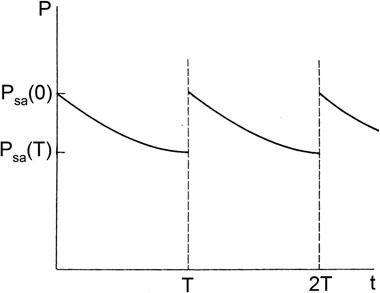
\includegraphics[width=0.55\textwidth]{855.png}
  \caption{Pulso arterial sistémico a partir del modelo idealizado (De [34]).}
  \label{fig:855}
\end{SCfigure}



Podemos determinar estas presiones en términos del volumen sistólico utilizando (\ref{eq:858})--(\ref{eq:860}) y (\ref{eq:866})
\begin{equation}
V_{\text{sa}}(0) = V_{\text{sa,d}} + C_{\text{sa}} P_{\text{sa}}(0)
\label{eq:8102}
\end{equation}
\begin{equation}
V_{\text{sa}}(T) = V_{\text{sa,d}} + C_{\text{sa}} P_{\text{sa}}(T).
\label{eq:8103}
\end{equation}
La diferencia es el volumen sistólico
\begin{equation}
V_{\text{stroke}} = V_{\text{sa}}(0) - V_{\text{sa}}(T) = C_{\text{sa}}(P_{\text{sa}}(0) - P_{\text{sa}}(T)) = C_{\text{sa}} P_{\text{sa}}(0) [1 - \exp(- T/\tau)].
\label{eq:8104}
\end{equation}
En consecuencia, encontramos
\begin{equation}
P_{\text{systole}} = P_{\text{sa}}(0) = \frac{V_{\text{stroke}}}{C_{\text{sa}} [1 - \exp(- T/\tau)]}
\label{eq:8105}
\end{equation}
\begin{equation}
P_{\text{diastole}} = P_{\text{sa}}(T) = \frac{V_{\text{stroke}} \exp(- T/\tau)}{C_{\text{sa}} [1 - \exp(- T/\tau)]}.
\label{eq:8106}
\end{equation}
Con (\ref{eq:893}) vemos que
\begin{equation}
P_{\text{pulse}} = P_{\text{systole}} - P_{\text{diastole}} = \frac{V_{\text{stroke}}}{C_{\text{sa}}}
\label{eq:8107}
\end{equation}
y por lo tanto $P_{\text{systole}}$, $P_{\text{diastole}}$, $V_{\text{stroke}}$, la frecuencia cardíaca $1/T$, $C_{\text{sa}}$ y $R_{\text{s}}$ ($= \tau/C_{\text{sa}}$) están todos interrelacionados.

Consideremos un ejemplo numérico. Para $V_{\text{stroke}} = 70\text{ cm}^3 = 0{,}070\text{ L}$ y $P_{\text{pulse}} = 40\text{ mmHg}$, la ecuación (\ref{eq:8104}) da $C_{\text{sa}} = V_{\text{stroke}}/P_{\text{pulse}} = 0{,}00175\text{ L/mmHg}$. Utilizando el valor de $R_{\text{s}}$ de la Tabla~8.8 de $17{,}5\text{ mmHg/(L/min)}$, sabemos que $\tau = R_{\text{s}} C_{\text{sa}} = 0{,}0306\text{ min}$. Con $T = 1/80\text{ min} = 0{,}0125\text{ min}$, las ecuaciones (\ref{eq:8105}) y (\ref{eq:8106}) proporcionan el último parámetro restante, el cual podría ser tanto $P_{\text{systole}}$ como $P_{\text{diastole}}$, ya que están relacionados mediante $P_{\text{pulse}} = P_{\text{systole}} - P_{\text{diastole}}$. A partir de (\ref{eq:8107}), obtenemos $P_{\text{systole}} = 120\text{ mmHg}$. Como se esperaba por autoconsistencia, $P_{\text{diastole}} = P_{\text{systole}} \exp(- T/\tau) = 120\text{ mmHg} \times \exp(- 0{,}0125\text{ min}/0{,}0306\text{ min}) = 80\text{ mmHg}$.

En el Problema~8.62 se describe un mejor modelo para el pulso arterial, en el cual el flujo de sangre desde el ventrículo izquierdo hacia las arterias sistémicas ocurre con una duración finita (no nula) en el ciclo cardíaco. Este proporciona predicciones que concuerdan mejor con la Fig.~8.53 que las de la Fig.~8.55. Incluso este modelo mejorado no explica el pequeño incremento de presión justo después de la sístole que se observa en las Figs.~8.5 y 8.53, el cual se conoce como la «incisura» o «muesca dícrota». Cuando la válvula semilunar se cierra, parte de la sangre que fluye hacia atrás rebota contra las paredes elásticas de la aorta, estableciendo una onda de presión en la aorta; este pico de presión se puede incluir con un refinamiento aún mayor en el modelo.

\begin{SCfigure}[0.9][htbp]
  \centering
  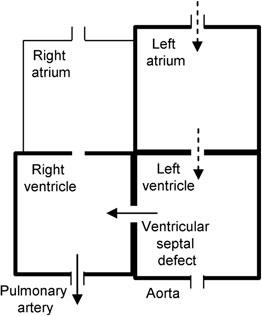
\includegraphics[width=0.5\textwidth]{862.png}
  \caption{Con un defecto septal ventricular (comunicación interventricular), la sangre fluye desde el ventrículo izquierdo hacia el derecho (Basado en [12]).}
  \label{fig:862}
\end{SCfigure}



\subsection{Modelo Windkessel}

Este modelo simplificado del pulso arterial también se conoce como el modelo Windkessel \cite{8}, el cual fue el primer modelo real del flujo sanguíneo. En este modelo, la sangre fluye desde el ventrículo izquierdo a un caudal $Q_{\text{in}}(t)$ hacia una cámara elástica de compliancia $C$ (es decir, las arterias más grandes) de volumen $V(t)$, y sale de ella a un caudal $Q_{\text{out}}(t)$ para ingresar a un elemento resistivo de resistencia $R_{\text{p}}$ (resistencia periférica de las arteriolas y capilares). Asume que todos los cambios de presión en las arterias ocurren al mismo tiempo. Debido a que la conservación del volumen para un fluido incompresible da
\begin{equation}
Q_{\text{in}}(t) = \frac{\mathrm{d}V(t)}{\mathrm{d}t} + Q_{\text{out}}(t),
\label{eq:8108}
\end{equation}
con $C = \mathrm{d}V(t)/\mathrm{d}P(t)$ (\ref{eq:857}) y $Q_{\text{out}}(t) = P(t)/R_{\text{p}}$ (\ref{eq:868}), la ecuación (\ref{eq:8108}) se convierte en
\begin{equation}
Q_{\text{in}}(t) = C \frac{\mathrm{d}P(t)}{\mathrm{d}t} + \frac{P(t)}{R_{\text{p}}}.
\label{eq:8109}
\end{equation}

La solución formal para esto es
\begin{equation}
P(t) = \exp(-t/\tau) \left( P(0) + \frac{1}{C} \int_{0}^{t} \exp(t'/\tau) Q_{\text{in}}(t') \mathrm{d}t' \right),
\label{eq:8110}
\end{equation}
donde $\tau = R_{\text{p}} C$. Se puede demostrar que esta es la solución mediante sustitución y por el método mostrado en el Apéndice~C. No obstante, resulta simple e instructivo examinar qué sucede después de la eyección ventricular, comenzando en $t = 0$ cuando $Q_{\text{in}}(t) = 0$ y $P = P(0)$, hasta que comienza el siguiente ciclo en $t = T$. Entonces,
\begin{equation}
\frac{\mathrm{d}P(t)}{\mathrm{d}t} + \frac{P(t)}{R_{\text{p}} C} = 0 \quad \text{para} \quad 0 < t < T.
\label{eq:8111}
\end{equation}
La solución es
\begin{equation}
P(t) = P(0) \exp(-t/\tau) \quad \text{para} \quad 0 < t < T,
\label{eq:8112}
\end{equation}
la cual es idéntica a (\ref{eq:8101}) (véase el Apéndice~C).

Este modelo Windkessel clásico de dos elementos es formalmente equivalente al circuito eléctrico, donde la resistencia eléctrica $R_{\text{elect}}$ se mapea como la resistencia al flujo en los capilares y la capacitancia eléctrica $C_{\text{elect}}$ se mapea como la compliancia de flujo (Tabla~D.1, Apéndice~D). (Así es como se expresa el modelo en la Fig.~8.56a). El voltaje $V_{\text{elect}}$ en el modelo eléctrico corresponde a la presión $P$ en el modelo de flujo y la corriente $I$ corresponde al caudal volumétrico $Q$. La ley de Ohm relaciona $V_{\text{elect}}$ e $I$ a través del resistor mediante $V_{\text{elect}} = I R_{\text{elect}}$. El voltaje a través del capacitor es $V_{\text{elect}} = q/C_{\text{elect}}$, donde la carga en el capacitor es $q$. Los voltajes a través de ambos elementos suman cero (segunda ley de Kirchhoff, Cap.~12), de modo que $I R_{\text{elect}} + q/C_{\text{elect}} = 0$. Debido a que $I = \mathrm{d}q/\mathrm{d}t$, tenemos $(\mathrm{d}q/\mathrm{d}t) R_{\text{elect}} + q/C_{\text{elect}} = 0$ o bien, con $V_{\text{elect}} = q/C_{\text{elect}}$,
\begin{equation}
\frac{\mathrm{d}V_{\text{elect}}}{\mathrm{d}t} + \frac{V_{\text{elect}}}{R_{\text{elect}} C_{\text{elect}}} = 0.
\label{eq:8113}
\end{equation}

\begin{figure}[htbp]
  \centering
  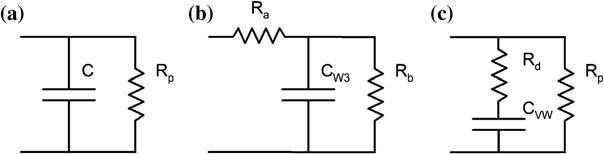
\includegraphics[width=0.8\textwidth]{856.png}
  \caption{Análogos eléctricos de a) un modelo Windkessel clásico o elástico (W2), b) un modelo Windkessel de tres elementos (o mejorado) (W3), y c) un modelo Windkessel viscoelástico (VW). Las resistencias eléctricas representan resistencias al flujo y las capacitancias eléctricas representan compliancias de flujo (Véase el Apéndice~D).}
  \label{fig:856}
\end{figure}



El modelo Windkessel de dos elementos se puede refinar agregando más elementos al análogo eléctrico. El modelo Windkessel de tres elementos mostrado en la Fig.~8.56b predice un pulso arterial más realista. La resistencia vascular $R_{\text{a}}$ de la aorta se agrega en serie, y el valor de la resistencia en paralelo es ahora $R_{\text{b}}$, la cual es igual a $R_{\text{p}} - R_{\text{a}}$. El modelo Windkessel viscoelástico (Fig.~8.56c) representa un tipo diferente de mejora del modelo Windkessel de dos elementos. Los sistemas arteriales compliantes están representados por una capacitancia (en el análogo eléctrico de la compliancia de flujo) que está en serie con una resistencia $R_{\text{d}}$, la cual representa el movimiento viscoso de la pared para representar más plenamente la viscoelasticidad de la aorta.

\subsection{Modelado del mal funcionamiento del corazón}

Existen muchas razones y formas en las que un corazón puede fallar \cite{46}. Por ejemplo, mutaciones individuales que truncan la proteína del sarcómero titina (Cap.~5) pueden provocar cambios en el tamaño, la forma y la función del corazón (lo que también se conoce como remodelación cardíaca), y pueden causar insuficiencia cardíaca temprana y muerte, incluyendo la miocardiopatía dilatada \cite{33}. Estas condiciones se pueden caracterizar cuantitativamente y, en principio, pueden incluirse en nuestros modelos del corazón y la circulación. El rendimiento cardíaco se puede caracterizar mediante varios parámetros, tales como el volumen sistólico $V_{\text{stroke}}$ y el gasto cardíaco $Q_{\text{t}} = F V_{\text{stroke}}$, descritos anteriormente.

La Figura~8.57 muestra el rendimiento cardíaco en función de las condiciones al final de la diástole en el ventrículo izquierdo. La curva intermedia describe el funcionamiento del corazón de esa persona, y el punto a representa a esa persona normal en reposo. En la insuficiencia cardíaca sistólica, como después de un infarto de miocardio, la curva se desplaza hacia abajo debido a una menor contractilidad del ventrículo izquierdo. El punto b representa a la persona descrita por el punto a después de la insuficiencia cardíaca. El aumento del volumen circulatorio en esta persona está representado por el punto c. El volumen sistólico aumenta debido a una mayor contractilidad en la curva superior, tal vez provocada por la infusión del fármaco norepinefrina.

\begin{figure}[htbp]
  \centering
  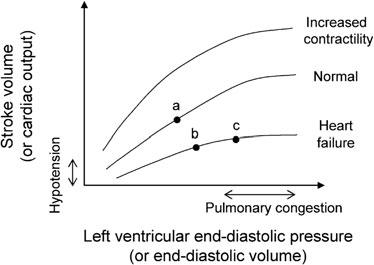
\includegraphics[width=0.7\textwidth]{857.png}
  \caption{Las curvas de rendimiento del ventrículo izquierdo (Frank-Starling) relacionan el rendimiento cardíaco con las condiciones previas (precarga), tales como la presión o el volumen del ventrículo izquierdo después de la diástole (Basado en [18]).}
  \label{fig:857}
\end{figure}



Los bucles de presión-volumen de línea sólida en la Fig.~8.58 representan el funcionamiento normal del corazón y son representaciones más precisas que la rectangular simplificada que se describe en nuestro modelo en la Fig.~8.51. En la disfunción sistólica, la curva de presión-volumen al final de la sístole (también conocida como la «relación presión-volumen al final de la sístole», ESPVR) se desplaza de 1 a 2 en a) debido a la disminución de la contractilidad cardíaca. Como se observa en el bucle discontinuo, el volumen al final de la sístole aumenta. En la disfunción diastólica, la curva de presión-volumen al final de la diástole («relación presión-volumen al final de la diástole», EDPVR) se desplaza de 1 a 2 en b) debido al aumento de la rigidez (disminución de la compliancia). Como se observa en el bucle discontinuo, la presión ventricular es más alta de lo normal para cualquier volumen diastólico. Con el avance de la edad, hay pocos cambios en la función sistólica, pero se presentan cambios importantes en la función diastólica. Existe un llenado diastólico temprano reducido, lo cual es compensado por un mayor llenado al final de la diástole. Esto puede hacer que las personas sean más propensas a desarrollar insuficiencia cardíaca congestiva \cite{1, 19}.

\begin{figure}[htbp]
  \centering
  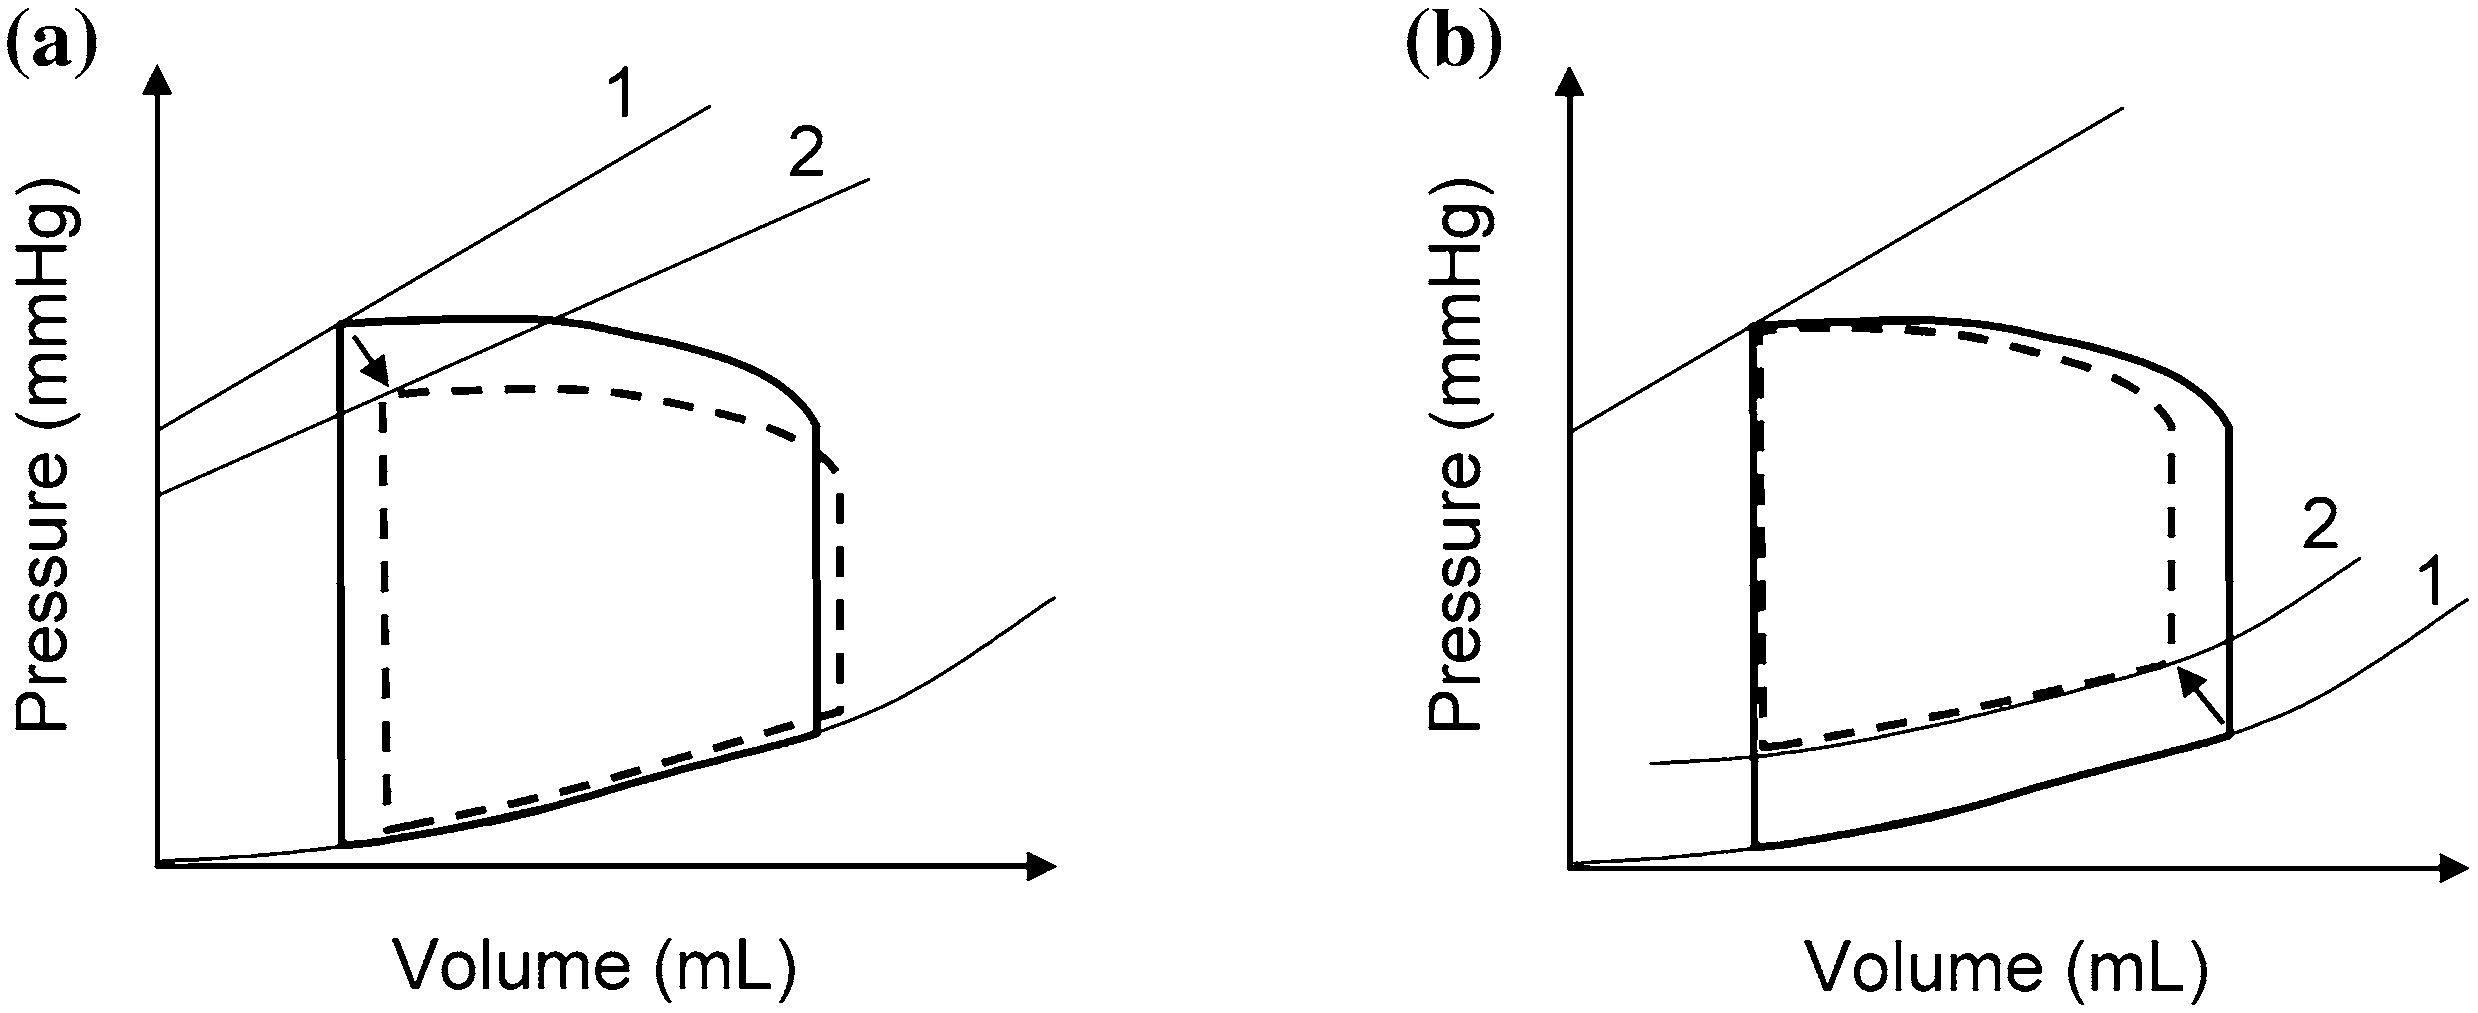
\includegraphics[width=0.8\textwidth]{858.png}
  \caption{Curvas de presión-volumen para el ventrículo izquierdo para un rendimiento normal (bucle sólido), disfunción sistólica (bucle discontinuo en a)) y disfunción diastólica (bucle discontinuo en b)) (Basado en [18]).}
  \label{fig:858}
\end{figure}



En la Fig.~8.59 se muestran los bucles de presión-volumen discontinuos para varios trastornos cardíacos. Las tres miocardiopatías descritas en a--c) se caracterizan por cambios en las curvas de presión-volumen al final de la sístole y de la diástole, como en los gráficos de la Fig.~8.58. En la miocardiopatía dilatada (DCM), el ventrículo izquierdo se dilata sin que necesariamente se vuelva más grueso. Como se observa en a), los volúmenes ventriculares al final de la sístole y de la diástole son mayores que los de un corazón normal, incrementándose más el volumen al final de la sístole, lo que conduce a una disminución neta en el volumen sistólico y a una variación mínima en las presiones. La ley de Laplace muestra que se necesita una mayor tensión en la pared del ventrículo para mantener la misma presión para la eyección de sangre debido a que el radio del ventrículo es mayor en la DCM, por lo que una persona con DCM utiliza más potencia para bombear el mismo volumen de sangre \cite{40}. En la miocardiopatía hipertrófica (HCM) (una causa de la hipertrofia ventricular izquierda), la masa del ventrículo izquierdo aumenta, a veces junto con su tamaño. Como se observa en b), esto conduce a un desplazamiento de la curva al final de la sístole y a una disminución de la compliancia sistólica, lo que hace que la presión aumente, y a una disminución de la compliancia diastólica a volúmenes mayores. El volumen sistólico disminuye debido a que el volumen al final de la diástole disminuye y el volumen después de la sístole aumenta. En la miocardiopatía restrictiva (RCM), el ventrículo izquierdo se vuelve rígido pero no necesariamente más grueso, lo cual a veces se debe a tejido cicatricial. Como se observa en c), la presión sistólica ventricular permanece normal, la presión diastólica aumenta y el volumen sistólico disminuye. (Estas miocardiopatías han sido responsables de las muertes tempranas de varios atletas de alto perfil).

\begin{figure}[htbp]
  \centering
  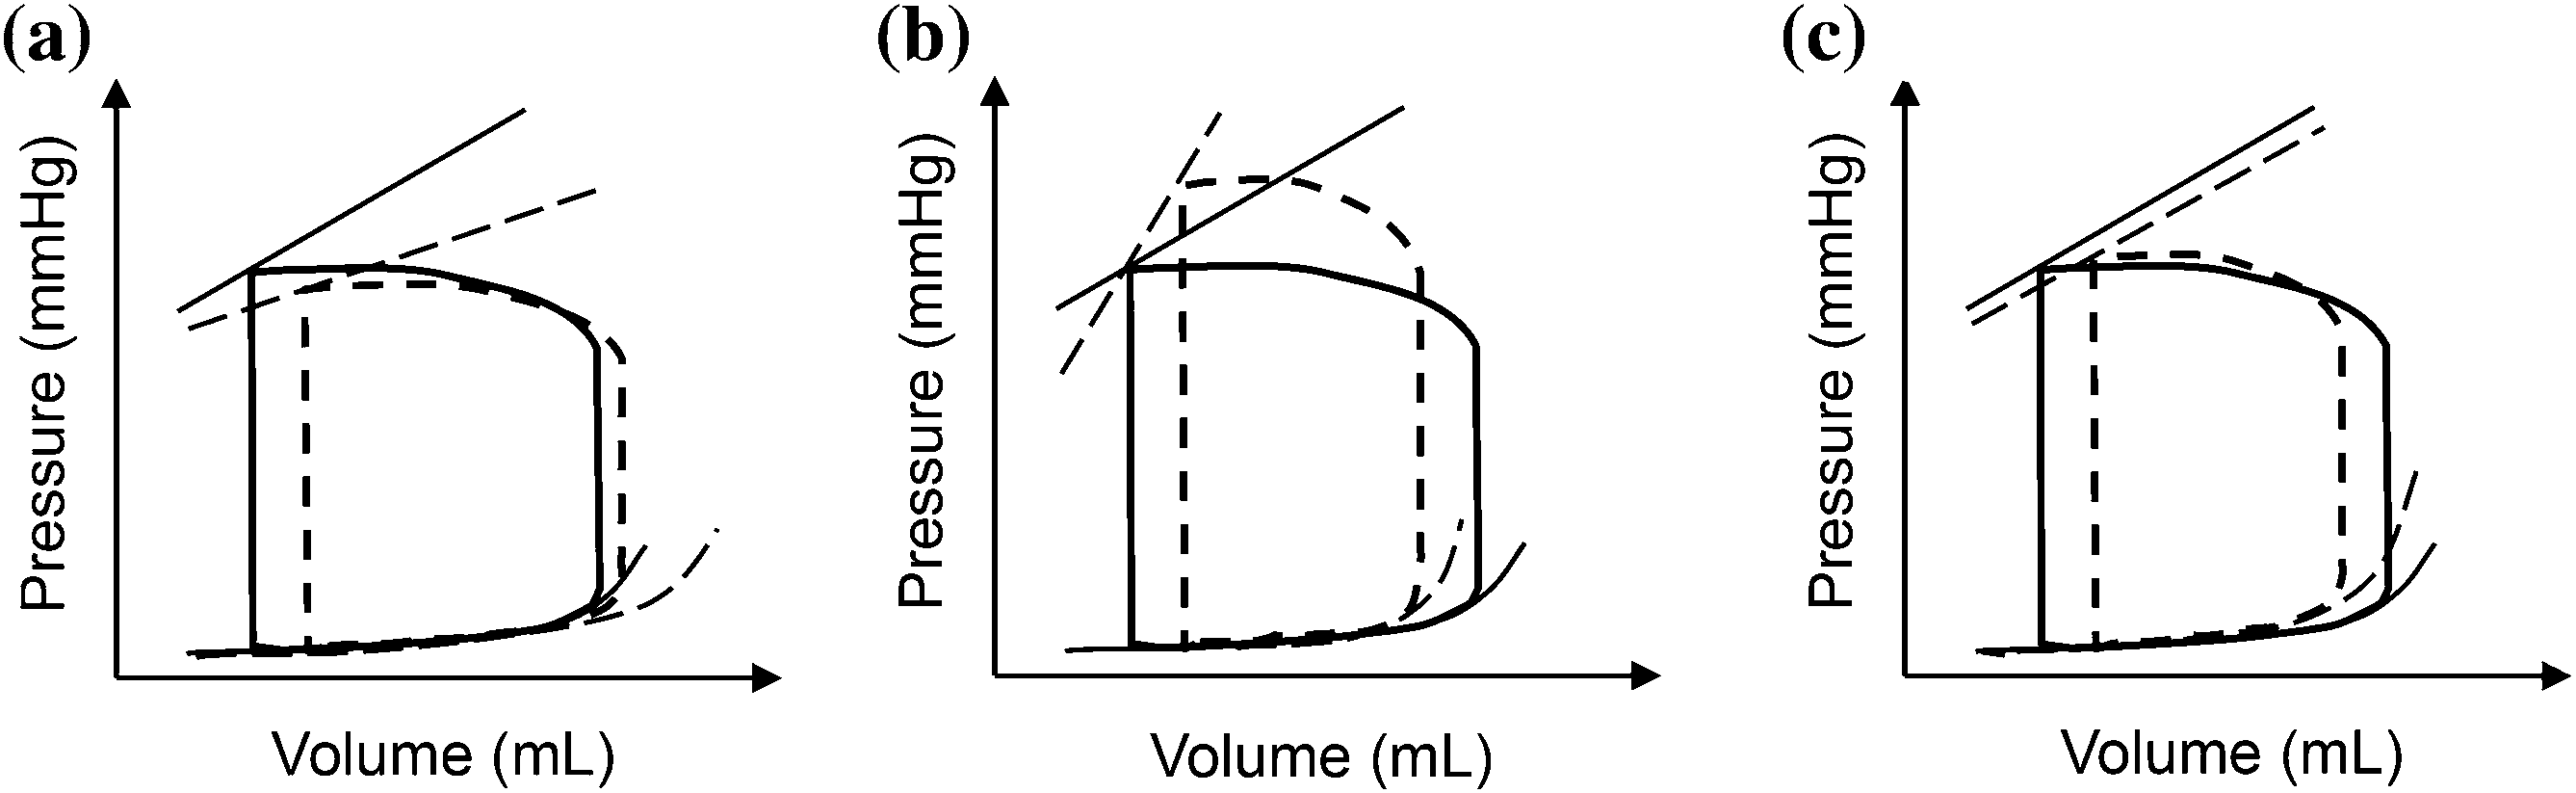
\includegraphics[width=0.8\textwidth]{859.png}
  \caption{Curvas de presión-volumen para el ventrículo izquierdo para un rendimiento normal (bucle sólido) y para varias anomalías cardíacas (bucle discontinuo). Se muestran las curvas de presión-volumen al final de la sístole (superior) y de la diástole (inferior) en a--c) para el corazón normal (curva sólida) y enfermo (curva discontinua). En la miocardiopatía dilatada (DCM) (a), la ESPVR se desplaza hacia la derecha y tiene una pendiente disminuida, mientras que la EDPVR se desplaza hacia la derecha. En la miocardiopatía hipertrófica (HCM) (b), la ESPVR se desplaza hacia la izquierda y tiene una pendiente aumentada, mientras que la EDPVR se desplaza hacia la izquierda. En la miocardiopatía restrictiva (RCM) (c), la ESPVR se desplaza hacia la derecha y tiene una pendiente sin cambios, mientras que la EDPVR tiene una pendiente aumentada (Basado en [35]).}
  \label{fig:859}
\end{figure}



Los efectos de las aortas estrechadas (estenosis aórtica) y de los orificios de la válvula mitral estrechados (estenosis mitral) se muestran en la Fig.~8.60. En la estenosis aórtica, la presión del ventrículo izquierdo es mucho mayor que la presión aórtica durante la eyección del ventrículo izquierdo. El volumen después de la sístole y el volumen y la presión después de la diástole aumentan, y el volumen sistólico disminuye. En la estenosis mitral, se presenta un llenado diastólico reducido, lo que conduce a una disminución del volumen sistólico y de la presión aórtica.

\begin{figure}[htbp]
  \centering
  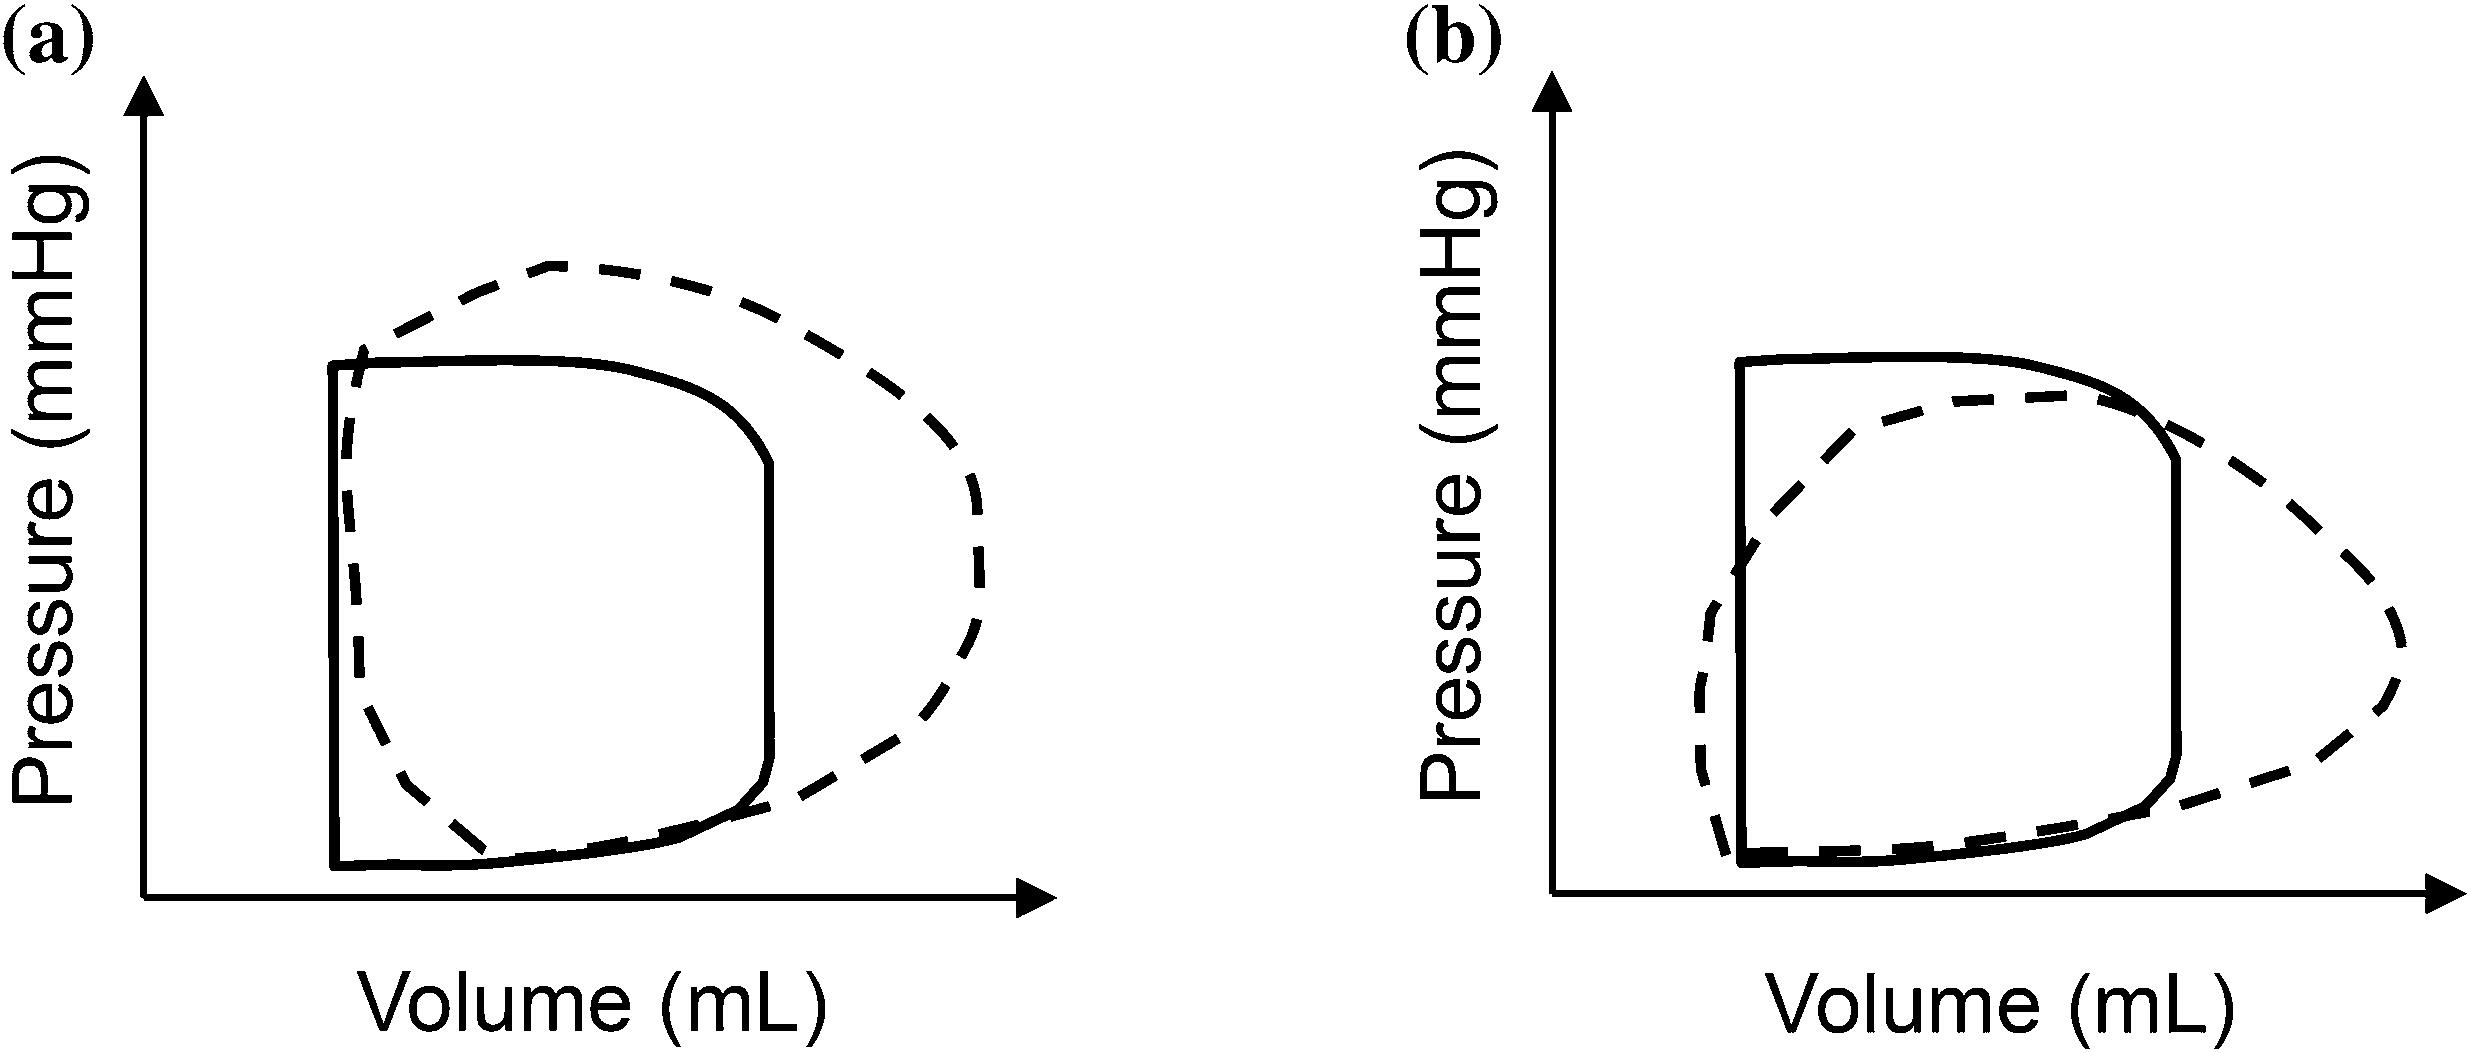
\includegraphics[width=0.8\textwidth]{860.png}
  \caption{Curvas de presión-volumen para el ventrículo izquierdo para un rendimiento normal (bucle sólido) y para las enfermedades valvulares a) estenosis aórtica y b) estenosis mitral (bucle discontinuo) (Basado en [35]).}
  \label{fig:860}
\end{figure}



Se presentan varias series de problemas cuando existen fugas entre las cavidades cardíacas. En la insuficiencia valvular (o regurgitación) hay un flujo retrógrado a través de una de las válvulas cardíacas, tales como la insuficiencia aórtica y la insuficiencia mitral en las válvulas del corazón izquierdo (Fig.~8.61). La fracción de regurgitación para la insuficiencia mitral es el volumen de sangre que fluye hacia atrás a través de la válvula mitral dividido por el volumen sistólico del ventrículo izquierdo. También puede haber aberturas en el tabique (septo) entre las aurículas o los ventrículos, lo que se denomina comunicación interauricular o interventricular (defecto septal) \cite{12}. Por ejemplo, una comunicación interventricular (defecto septal ventricular) es una condición congénita en la cual existe una abertura entre los ventrículos izquierdo y derecho (Fig.~8.62). Durante la sístole, la sangre fluye desde el ventrículo izquierdo hacia el derecho debido a la mayor presión en el primero. Esto conduce a un aumento del retorno sanguíneo al lado izquierdo del corazón, lo que provoca el agrandamiento de la aurícula y del ventrículo izquierdos. La fracción de eyección (EF) es el volumen sistólico dividido por el volumen ventricular al final de la diástole (cuando el ventrículo está lleno). Normalmente es del $55\text{--}75\%$, pero puede ser menor con un defecto septal.

\begin{figure}[htbp]
  \centering
  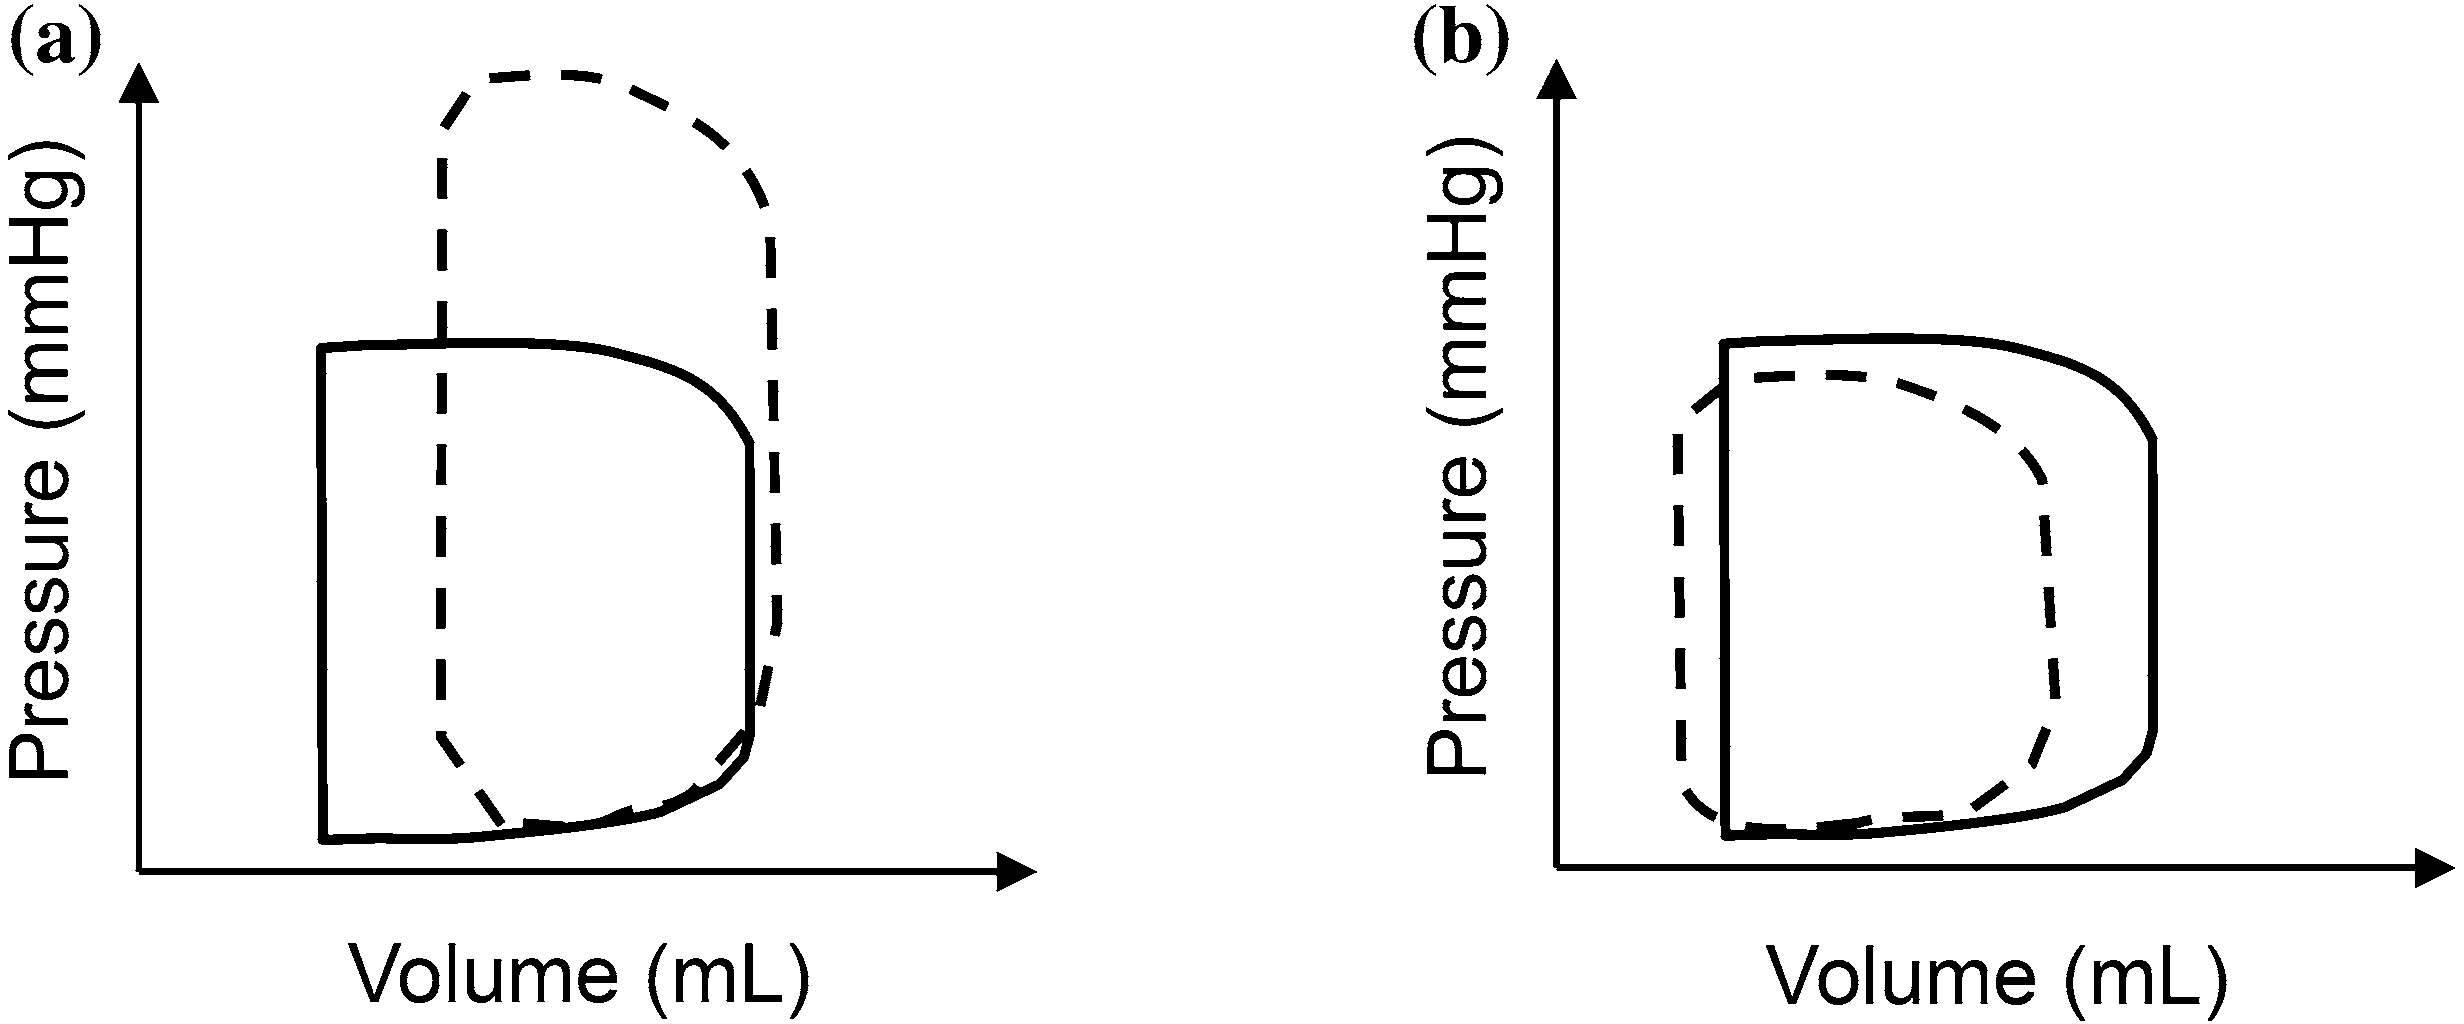
\includegraphics[width=0.8\textwidth]{861.png}
  \caption{Curvas de presión-volumen para el ventrículo izquierdo para un rendimiento normal (bucle sólido) y para a) insuficiencia aórtica y b) insuficiencia mitral (bucle discontinuo) (Basado en [35]).}
  \label{fig:861}
\end{figure}



\section{Resumen}

El flujo de sangre en los vasos del sistema circulatorio se puede modelar utilizando la naturaleza resistiva y compliante del flujo. Esto se puede combinar con un modelo del corazón para comprender el flujo en todo el sistema circulatorio. Estos modelos también se pueden utilizar para comprender las consecuencias físicas de un mal funcionamiento del corazón y de los problemas en el sistema circulatorio, tales como arterias obstruidas y debilitadas, que pueden provocar accidentes cerebrovasculares y aneurismas. La energía necesaria para hacer funcionar el corazón también se puede modelar.

\section*{Problemas}

\subsection*{Presión sanguínea}

\textbf{8.1} (a) El cerebro de un ser humano está $55\text{ cm}$ por encima del corazón. Si la presión arterial promedio en las arterias principales cerca del corazón es de $100\text{ mmHg}$, ¿cuál es la presión arterial en las arterias principales del cerebro (tanto en $\text{mmHg}$ como en $\text{cmH}_2\text{O}$) cuando una persona está acostada o de pie?

(b) Repita la parte (a) para un ser humano erguido en la Luna ($g = g_{\text{Tierra}}/6$) y en Júpiter ($g = 2{,}34 g_{\text{Tierra}}$).

(c) Un piloto al salir de una picada experimenta una aceleración centrípeta hacia arriba $a$ de magnitud $v^2/r$, donde $v$ es la velocidad del avión y $r$ es el radio de curvatura de la trayectoria, la cual se suma a la gravedad (aumentando efectivamente $g$ a $g + a$). ¿Cuál es la presión arterial en el cerebro del piloto para $v = 200\text{ m/s}$ y $r = 2\text{ km}$? ¿Qué le podría suceder al piloto durante esta recuperación de la picada? ¿Esperaría mareos debido a la falta de sangre en la cabeza? (Véase la Fig.~8.63).

\begin{figure}[htbp]
  \centering
  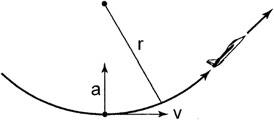
\includegraphics[width=0.8\textwidth]{863.png}
  \caption{Trayectoria de un piloto saliendo de una picada, con los vectores de aceleración y velocidad mostrados para el punto más bajo de la picada. Para el Problema 8.1 (De [4]).}
  \label{fig:863}
\end{figure}



\textbf{8.2} En el Problema~8.1d vimos que la presión de la sangre que sale del corazón de una jirafa e ingresa a su sistema sistémico debe ser mucho mayor que la de los humanos debido a su largo cuello.

(a) ¿Una presión arterial de $280\text{ mmHg}/180\text{ mmHg}$ explicaría el bombeo de la sangre hacia arriba de este largo cuello en las arterias grandes y luego la caída de presión que ocurre en las arterias muy pequeñas en el cerebro?

(b) La jirafa tiene esta presión arterial relativamente alta debido a este cuello largo, el cual usualmente es casi vertical. Sin embargo, podríamos esperar que hubiera una afluencia de sangre al cerebro debido a esta alta presión cuando la jirafa baja la cabeza casi $7\text{ m}$ al agacharse para beber agua, y que esto podría conducir a la ruptura de las arterias en el cerebro. ¿Por qué?

(c) Tal ruptura de arterias no ocurre debido a efectos compensatorios. Explique esto considerando lo siguiente: (i) Las paredes elásticas de la larga arteria carótida de la jirafa ayudan a impulsar la sangre hacia arriba (lo cual es una acción peristáltica), y esto también significa que esta arteria puede hincharse para absorber el exceso de sangre cuando baja la cabeza debido a que es muy compliante. (ii) La vena yugular de la jirafa contiene una serie de válvulas unidireccionales que evitan el flujo retrógrado de la sangre cuando la cabeza de la jirafa está abajo.

\textbf{8.3} Cuando usted se para de cabeza, ¿por qué se le pone la cabeza roja y por qué las piernas se le ponen pálidas?

\textbf{8.4} ¿Por qué se mide la presión arterial utilizando las arterias principales del brazo y no las del antebrazo o de la pierna?

\textbf{8.5} Le dicen que su presión arterial es de $880\text{ mmHg}/840\text{ mmHg}$. Usted está comprensiblemente preocupado porque estos valores son astronomicamente altos, pero le dicen que no se preocupe porque su presión arterial es normal. ¿Debería estar preocupado?

\textbf{8.6} (a) Se realiza una infusión intravenosa por gravedad. Si el fluido a suministrar tiene una densidad de $1{,}0\text{ g/cm}^3$, ¿a qué altura por encima de la vena, $h$, debe colocarse la superficie superior del fluido en la botella para que el fluido apenas entre en la vena? La presión manométrica en la vena es de $18\text{ mmHg}$. (Asuma que la aguja que entra en la vena tiene un diámetro interno «grande»). (Véase la Fig.~8.64).

\begin{figure}[htbp]
  \centering
  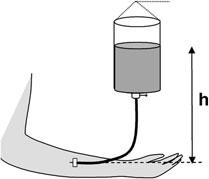
\includegraphics[width=0.7\textwidth]{864.png}
  \caption{Infusión intravenosa por gravedad. (Basado en [26]). Para el Problema 8.6.}
  \label{fig:864}
\end{figure}



(b) Si esta aguja tiene un diámetro interno «muy pequeño», ¿debería colocarse la botella más arriba, más abajo o a la misma altura? ¿Por qué?

(c) ¿Por qué tales inyecciones se realizan por vía intravenosa y no intraarterial?

\textbf{8.7} Usted está acostado y se lesiona de tal manera que la sangre de una arteria principal sale disparada hacia arriba. ¿Qué tan alto puede salir disparada?

\textbf{8.8} Gire un brazo tan rápido como pueda muchas veces hasta que vea que los dedos de ese brazo se ponen rojos. (Continúe incluso si no los ve ponerse más rojos). [2]

(a) Estime la aceleración centrífuga en el extremo de las puntas de sus dedos, $v_{\text{radial}}^2/r = v_{\text{radial}}^2/l_{\text{arm}}$, donde $l_{\text{arm}}$ es la longitud de su brazo (hasta las puntas de sus dedos) y $v_{\text{radial}}$ es la velocidad radial de las puntas de sus dedos. (¿Por qué $v_{\text{radial}} = 2\pi l_{\text{arm}}/T$, donde $T$ es el período para un ciclo completo de este movimiento?)

(b) Exprese esta aceleración en unidades de $g$.

(c) Calcule la presión efectiva que empuja la sangre hacia sus dedos mediante este movimiento. Esta es la fuerza aparente hacia afuera dividida por el área de sección transversal de sus dedos, $A_{\text{dedos}}$:
\begin{equation*}
P = \frac{m_{\text{dedos}} v_{\text{radial}}^2 / l_{\text{brazo}}}{A_{\text{dedos}}}.
\end{equation*}
Debido a que $m_{\text{dedos}} = \rho_{\text{dedos}} l_{\text{dedos}} A_{\text{dedos}}$, esta presión es:
\begin{equation*}
P = \rho_{\text{dedos}} v_{\text{radial}}^2 \left(\frac{l_{\text{dedos}}}{l_{\text{brazo}}}\right).
\end{equation*}

(d) Compare esto con la presión sistólica de $120\text{ mmHg}$ y explique por qué sus dedos se pusieron (podrían haber o deberían haber) rojos.

\subsection*{Caída de presión sanguínea durante el flujo}

\textbf{8.9} Para las arterias más pequeñas, ¿qué tanto mayor es el área de sección transversal total de los dos vasos hijos que la del vaso madre?

\textbf{8.10} Calcule la caída de presión (en $\text{mmHg}$) a través de los siguientes sistemas arteriales utilizando la ley de Poiseuille con $\eta_{\text{blood}} = 4 \times 10^{-3}\text{ Pa}\cdot\text{s}$, para un flujo total de $80\text{ cm}^3\text{/s}$ a través de cada sistema:

(a) aorta (radio interno $r = 1{,}25\text{ cm}$, longitud $L = 10\text{ cm}$, todo el flujo en esta única aorta)

(b) arterias grandes ($r = 0{,}2\text{ cm}$, $L = 75\text{ cm}$, $n = 200$ de ellas, cada una con el mismo flujo y las mismas dimensiones)

(c) arterioles ($r = 30\text{ }\mu\text{m}$, $L = 0{,}6\text{ cm}$, $n = 5 \times 10^5$)

(d) capilares ($r = 3{,}5\text{ }\mu\text{m}$, $L = 2\text{ mm}$, $n = 10^{10}$).

\textbf{8.11} Al estimar las caídas de presión a través de las diferentes ramificaciones arteriales, asumimos números específicos de arterias de diámetros y longitudes dados. En realidad, existe un amplio rango de diámetros y longitudes arteriales. ¿Cómo afecta esto a las caídas de presión en el sistema arterial sistémico?

\textbf{8.12} Al estimar las caídas de presión a través de las arteriolas, asumimos un número específico de arteriolas con el mismo diámetro y longitud.

(a) Supongamos que todas las arteriolas tienen el mismo radio, pero sus longitudes (en lugar de ser todas $L$) varían entre $0{,}8L$ y $1{,}2L$ (con igual probabilidad en todo el rango). ¿Cómo cambia esto la resistencia total del sistema de arteriolas?

(b) Supongamos que todas las arteriolas tienen la misma longitud, pero sus radios (en lugar de ser todos $r$) varían entre $0{,}8r$ y $1{,}2r$ (con igual probabilidad en todo el rango). ¿Cómo cambia esto la resistencia total del sistema de arteriolas?

(c) La caída de presión a través de cada arteriola en el sistema debe ser la misma porque cada una es alimentada por las arterias grandes, cuya presión es establecida por el ventrículo izquierdo, y por el lado arterial de los capilares, cuya presión también está establecida. Si la caída de presión total a través de las arteriolas no cambia (debido a los cambios en (a) o (b)), ¿cómo cambia el caudal total en el sistema de arteriolas y cuál es el flujo en cada arteriola, para las situaciones descritas alternativamente en (a) y (b)?

(d) Si se deseara que el caudal se mantuviera igual en cada arteriola en (a) y (b) para las distribuciones dadas de longitudes y radios, ¿cómo se tendrían que cambiar las distribuciones de radios y longitudes en cada una, respectivamente?

\textbf{8.13} Encuentre la caída de presión a través de las arteriolas en el Problema~8.10c si, con el mismo flujo total en ambos casos, ocurre que:

(a) todas las arteriolas se obstruyen de tal manera que sus radios disminuyen a $28\text{ }\mu\text{m}$, o

(b) el número de arteriolas disminuye a $4 \times 10^5$.

(c) ¿Cuánto tendría que cambiar la presión en las arterias principales si el cuerpo respondiera a cualquiera de los dos cambios manteniendo el mismo caudal?

\textbf{8.14} Asuma que el diámetro de cada vaso sanguíneo en una persona se duplica y que el caudal volumétrico total no cambia.

(a) ¿Cuál es el nuevo volumen total de sangre? (Asuma los parámetros de referencia de este capítulo).

(b) ¿Cuál es el nuevo tiempo de circulación de la sangre (que es el volumen total de sangre dividido por el caudal volumétrico total)?

(c) ¿Cómo cambian las resistencias de las arteriolas y los capilares?

(d) ¿Cómo cambian las caídas de presión a través de las arteriolas y los capilares?

(e) ¿Cómo cambia el trabajo realizado por el corazón?

\textbf{8.15} Repita el Problema~8.14 si, en su lugar, se duplica la longitud de cada vaso sanguíneo.

\textbf{8.16} La longitud de un vaso sanguíneo se duplica y su diámetro se duplica.

(a) ¿Cómo cambia la resistencia al flujo?

(b) Si el flujo a través de él no cambia, ¿cómo cambia la caída de presión?

(c) ¿Cómo cambia el flujo a través de él si, en su lugar, la caída de presión no cambia?

\textbf{8.17} Su temperatura corporal interna aumenta de $37$ a $40\text{ }^\circ\text{C}$. Suponiendo que lo único que cambia es la viscosidad de la sangre, ¿cómo debe cambiar la presión arterial para garantizar que el caudal permanezca sin cambios?

\subsection*{Caída de presión sanguínea durante el flujo}

\textbf{8.18} Utilice (\ref{eq:820}) para relacionar $P(L)$ con $P(0)$ y otros términos de flujo.

\textbf{8.19} (a) Estime cuánto cambia el flujo en las arterias pequeñas al incluir la influencia de la compliancia utilizando (\ref{eq:820}) y asumiendo la misma caída de presión.

(b) Repita esta estimación para determinar cuánto cambia la caída de presión con este análisis asumiendo el mismo caudal.

\textbf{8.20} Exprese las unidades de resistencia al flujo de $\text{N}\cdot\text{s/m}^5$ en términos de $(\text{N/m}^2)/(\text{cm}^3\text{/s})$, $\text{dina}\cdot\text{s/cm}^5$ y $\text{PRU}$ (con $1\text{ PRU} = 1\text{ mmHg}\cdot\text{s/mL}$).

\textbf{8.21} (a) Calcule la resistencia vascular periférica total en los sistemas sistémico y pulmonar para una persona con un caudal sanguíneo en estado estacionario de $5\text{ L/min}$, y con una presión arterial de $120/80\text{ mmHg}$ en el sistema sistémico y una presión de $25/8\text{ mmHg}$ en el sistema pulmonar. Exprese su respuesta en unidades de $\text{dina}\cdot\text{s/cm}^5$, que son unidades CGS y las que a menudo utilizan los cardiólogos.

(b) La expresión dada en el texto para esta resistencia al flujo vascular debe corregirse porque utiliza la presión promedio al principio del sistema en lugar de la caída de presión a través del sistema. Para el sistema sistémico, la presión final es la de la aurícula derecha ($2\text{ mmHg}$) y para el sistema pulmonar es la de la aurícula izquierda ($5\text{ mmHg}$). ¿Cómo afecta el uso de la caída de presión real a sus cálculos en la parte (a) (tanto cualitativa como cuantitativamente)?

\textbf{8.22} (a) La resistencia vascular pulmonar cambia con el volumen pulmonar. La Figura~8.65 muestra que esta aumenta considerablemente con volúmenes pulmonares más grandes, en parte porque los alvéolos más grandes estiran los capilares pulmonares. También aumenta con volúmenes pulmonares muy pequeños debido a que estos capilares que rodean los alvéolos se vuelven estrechos. Calcule el rango de caudales sanguíneos pulmonares (en $\text{L/min}$), asumiendo este rango de resistencias y asumiendo que las presiones pulmonares son las mismas que en el Problema~8.21.

\begin{figure}[htbp]
  \centering
  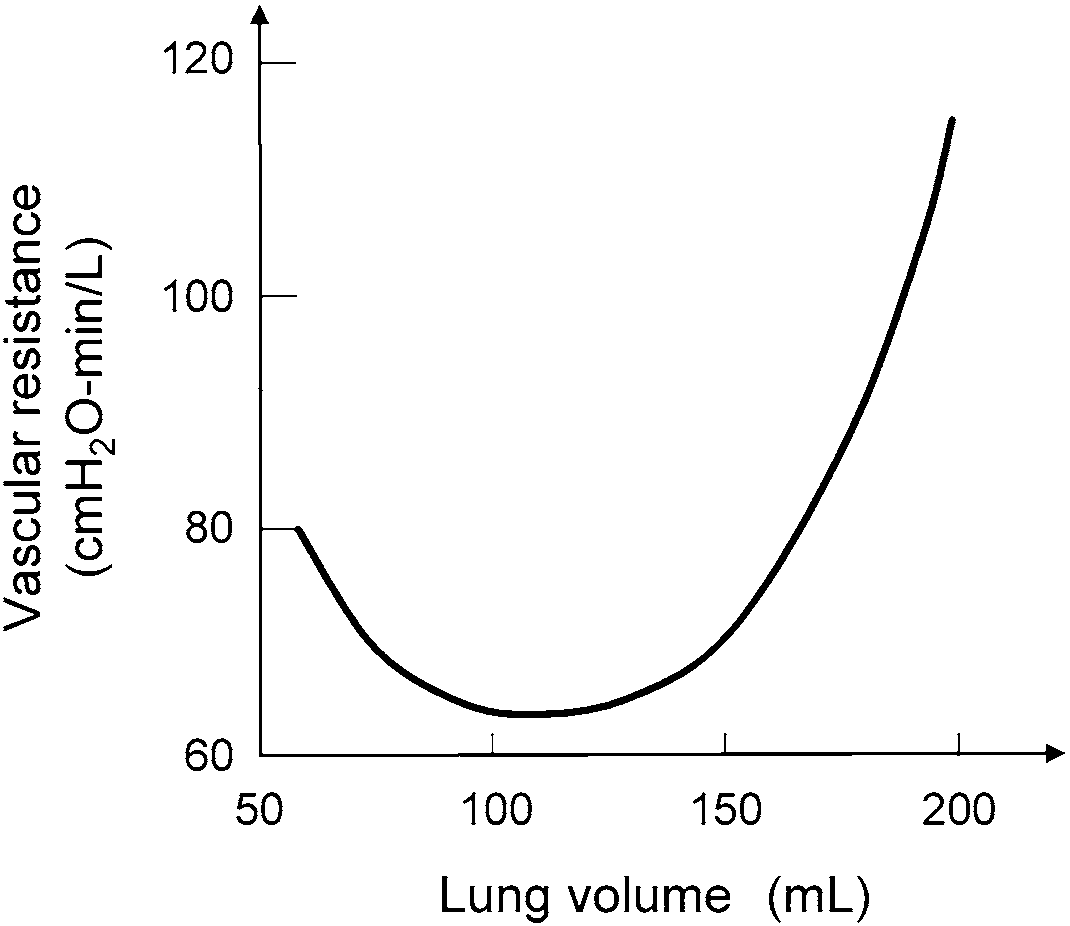
\includegraphics[width=0.7\textwidth]{865.png}
  \caption{Efecto del volumen pulmonar sobre la resistencia vascular pulmonar (flujo sanguíneo) (A partir de una preparación de lóbulo animal). (Basado en [69]). Para el Problema 8.22.}
  \label{fig:865}
\end{figure}



(b) Las presiones pulmonares en realidad cambian con el volumen pulmonar. Si cambiaran de manera que el flujo promedio se mantuviera igual al de un volumen pulmonar de $110\text{ mL}$, determine este cambio. (Para fines de este cálculo, asuma que la relación entre las presiones sistólica y diastólica permanece constante y que la presión de la aurícula izquierda se mantiene igual).

\textbf{8.23} (a) Determine las compliancias generales de los sistemas arterial y venoso sistémicos utilizando la Fig.~8.25.

(b) ¿Es razonable la relación entre estas dos compliancias, dado nuestro modelo de compliancia y los datos de los vasos en ambos grupos? (Considere únicamente los vasos grandes en ambos grupos).

\textbf{8.24} ¿Sugiere la Fig.~8.25 que la estimulación e inhibición simpáticas cambian las compliancias de los vasos, sus volúmenes muertos o ambos?

\textbf{8.25} Relacione la distensibilidad (introducida en el Cap.~7) con $C_{\text{flow}}$, $c_{\text{flow}}$ y $C'_{\text{flow}}$.

\textbf{8.26} Muestre que el término de corrección para (\ref{eq:819}) es $(c_{\text{flow}}^2/3A_{\text{d}}^2)((P(0))^2 + P(0)P(L) + (P(L))^2)$.

\textbf{8.27} (a) Muestre que (\ref{eq:820}) se puede obtener a partir de (\ref{eq:819}).

(b) Muestre que también se puede derivar mediante la integración de (\ref{eq:814}), expresada en $r$, utilizando (\ref{eq:87}).

\textbf{8.28} (a) Muestre que el término de corrección para (\ref{eq:820}), obtenido al integrar (\ref{eq:814}) expresada en $r$ y utilizando (\ref{eq:87}), es $(1/2)({C'_{\text{flow}}}^2/r_{\text{d}}^2)((P(0))^2 + P(0)P(L) + (P(L))^2)$.

(b) Muestre que cuando la corrección determinada a partir del enfoque de área (Problema~8.26) se expresa en términos de $r$, se convierte en $(1/3)({C'_{\text{flow}}}^2/r_{\text{d}}^2)((P(0))^2 + P(0)P(L) + (P(L))^2)$.

(c) ¿Por qué difiere esto del resultado en (a)?

\subsection*{Flujo y presión}

\textbf{8.29} ¿Cuál es el tiempo promedio que pasa la sangre en un capilar?

\textbf{8.30} El índice cardíaco es el gasto cardíaco dividido por el área de superficie de la persona. Normalmente varía entre $2{,}6$ y $4{,}2\text{ (L/min)/m}^2$. Utilice esto para determinar el gasto cardíaco de un ser humano promedio. ¿Cómo se compara este valor con el gasto cardíaco normal que hemos asumido?

\textbf{8.31} Una arteria de radio $r_1$ y velocidad de la sangre $u_1$ se divide en $n$ arterias de igual radio. Encuentre el radio $r_2$ y la velocidad de la sangre $u_2$ en estas arterias hijas, asumiendo que la caída de presión por unidad de distancia $\mathrm{d}P/\mathrm{d}x$ es la misma en la arteria inicial y en cada arteria hija.

\textbf{8.32} Cuatro venas de radio $r_1$ y velocidad de flujo $u_1$ se combinan para formar una vena con un radio $r_2 = 4r_1$. Encuentre la velocidad de flujo en la vena más grande.

\textbf{8.33} El radio de cada sección de la aorta y de las arterias ilíaca externa, femoral, subclavia y braquial disminuye como $\exp(-kx)$, donde $k$ es el factor de conicidad y $x$ es la distancia a lo largo del vaso. Utilice la Tabla~8.4 para encontrar el factor de conicidad $k$ para cada vaso \cite{57}.

\textbf{8.34} El diseño de los vasos sanguíneos a veces se optimiza minimizando una «función de costo», $F$, la cual es la suma de la tasa a la que se realiza trabajo sobre la sangre en el vaso y la tasa a la que se utiliza energía por el metabolismo a través de la sangre en el vaso \cite{24}. El primer término es $Q(\Delta P)$, para un caudal $Q$ y una caída de presión $\Delta P$, y se asume que el segundo término es proporcional al volumen del vaso de radio $r$ y longitud $L$, $K\pi r^2 L$, donde $K$ es una constante. En consecuencia, la función de costo se puede escribir como
\begin{equation}
F = Q(\Delta P) + K\pi r^2 L.
\label{eq:8114}
\end{equation}

(a) Para un vaso resistivo, muestre que esto se convierte en
\begin{equation}
F = \frac{8\eta L}{\pi r^4} Q^2 + K\pi r^2 L.
\label{eq:8115}
\end{equation}

(b) Para una longitud de vaso y un caudal fijos, muestre que el radio óptimo es
\begin{equation}
r_{\text{opt}} = \left( \frac{16\eta}{\pi^2 K} \right)^{1/6} Q^{1/3}
\label{eq:8116}
\end{equation}
y la función de costo mínima es
\begin{equation}
F_{\text{min}} = \frac{3\pi}{2} K L r_{\text{opt}}^2.
\label{eq:8117}
\end{equation}

\textbf{8.35} (problema avanzado) Utilizaremos la función de costo definida en el Problema~8.34 para optimizar el flujo en un vaso de radio $r_0$ y longitud $L_0$ con un caudal $Q_0$, que se bifurca en un vaso de radio $r_1$ y longitud $L_1$ con un caudal $Q_1$ a un ángulo $\theta$ con respecto al primer vaso y en otro de radio $r_2$ y longitud $L_2$ con un caudal $Q_2$ a un ángulo $\phi$ con respecto al primer vaso, como se observa en la Fig.~8.66a \cite{24}. Tener vasos rectos y coplanares minimiza las longitudes de los vasos.

\begin{figure}[htbp]
  \centering
  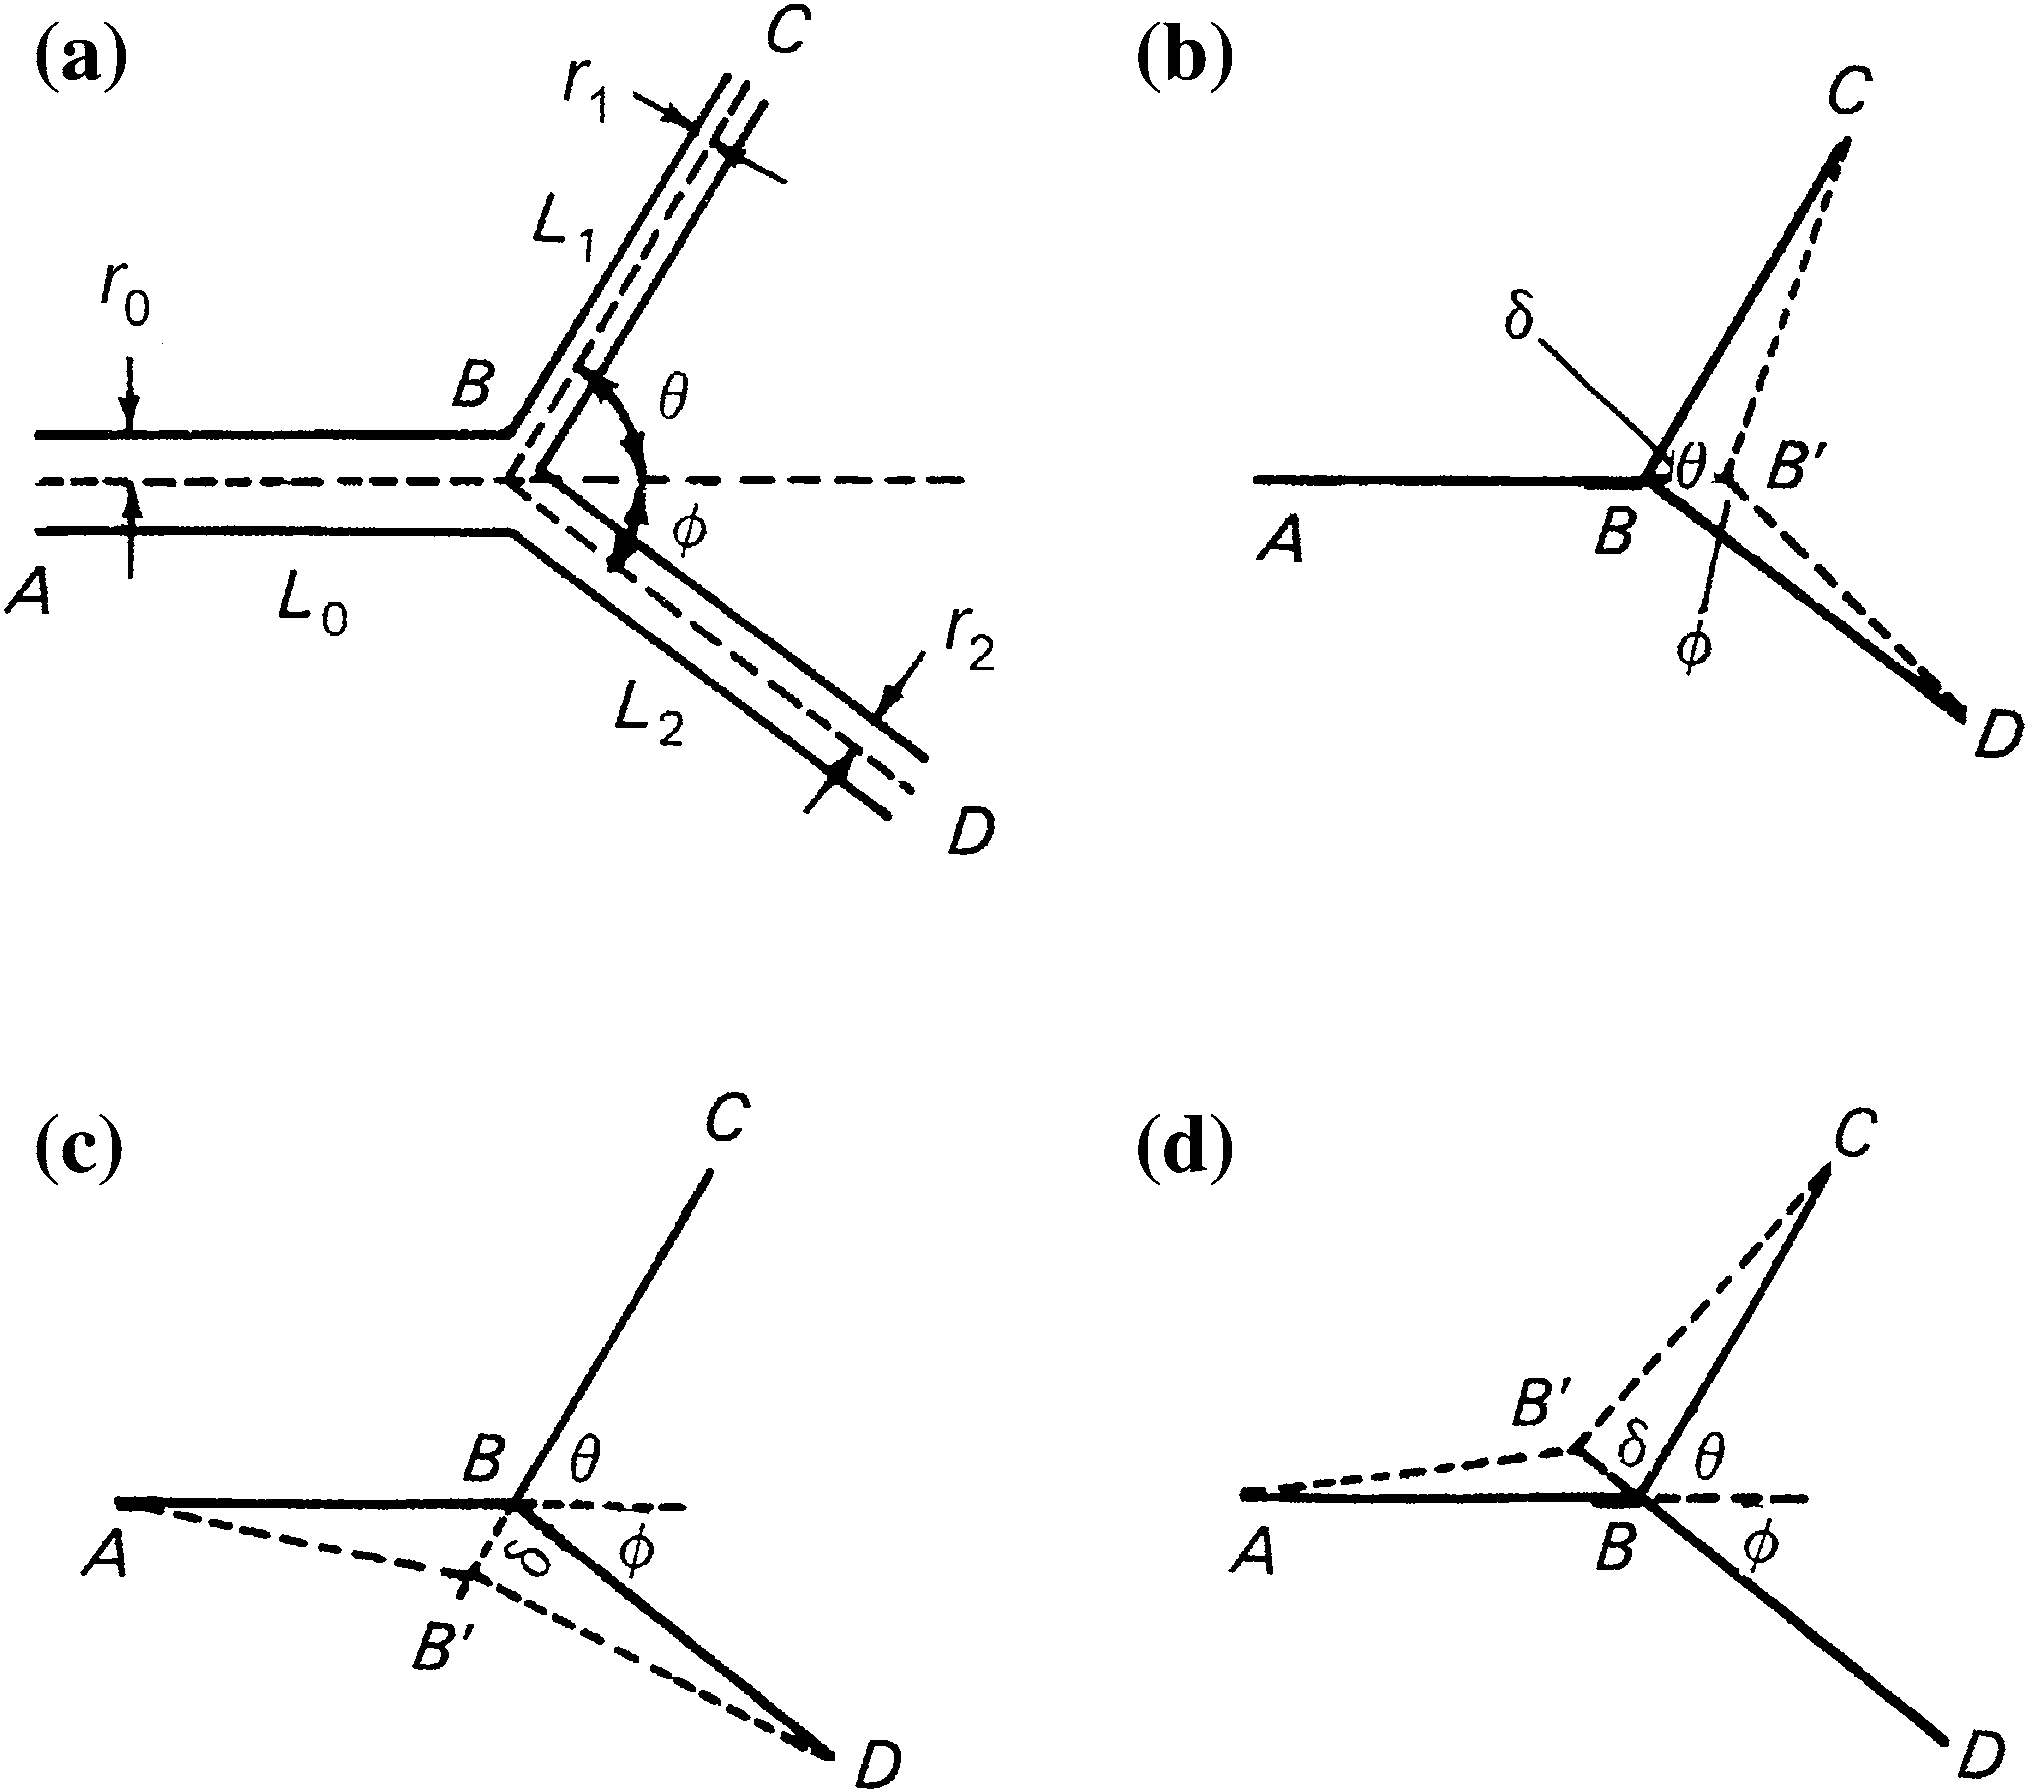
\includegraphics[width=0.7\textwidth]{866.png}
  \caption{a) Un vaso planar que se bifurca. Determinación de las variaciones en la longitud de cada vaso para pequeños desplazamientos planares de $B$ a $B'$ en las direcciones b) $AB$, c) $AC$ y d) $DB$ (Basado en \cite{24}). Para el Problema 8.35.}
  \label{fig:866}
\end{figure}



(a) Muestre que la función de costo total es
\begin{equation}
F_{\text{min}} = \frac{3\pi K}{2} (r_0^2 L_0 + r_1^2 L_1 + r_2^2 L_2).
\label{eq:8118}
\end{equation}

(b) Podemos optimizar las longitudes y los ángulos de los vasos considerando cómo los desplazamientos del punto $B$ en la Fig.~8.66b--d cambian la función de costo. Muestre que cualquier movimiento de este tipo del punto $B$ causa cambios de longitud $\delta L_0$, $\delta L_1$ y $\delta L_2$ que conducen a un cambio en la función de costo de
\begin{equation}
\delta F_{\text{min}} = \frac{3\pi K}{2} (r_0^2 (\delta L_0) + r_1^2 (\delta L_1) + r_2^2 (\delta L_2)).
\label{eq:8119}
\end{equation}
Esto se optimiza al establecer $\delta F_{\text{min,opt}} = 0$.

(c) Muestre que mover el punto $B$ a lo largo de $AB$ hacia $B'$ una distancia $\delta$, como se muestra en la Fig.~8.66b, da $\delta L_0 = \delta$, $\delta L_1 = -\delta \cos \theta$ y $\delta L_2 = -\delta \cos \phi$, y $\delta F_{\text{min,opt}} = (3\pi K\delta/2)(r_0^2 - r_1^2 \cos \theta - r_2^2 \cos \phi) = 0$, por lo que se optimiza mediante
\begin{equation}
r_0^2 = r_1^2 \cos \theta + r_2^2 \cos \phi.
\label{eq:8120}
\end{equation}

(d) Muestre que mover el punto $B$ a lo largo de $CB$ hacia $B'$ una distancia $\delta$, como se muestra en la Fig.~8.66c, da $\delta L_0 = -\delta \cos \theta$, $\delta L_1 = \delta$ y $\delta L_2 = \delta \cos(\theta + \phi)$, y $\delta F_{\text{min,opt}} = (3\pi K\delta/2)(-r_0^2 \cos \theta + r_1^2 + r_2^2 \cos(\theta + \phi)) = 0$, por lo que se optimiza mediante
\begin{equation}
-r_0^2 \cos \theta + r_1^2 + r_2^2 \cos(\theta + \phi) = 0.
\label{eq:8121}
\end{equation}

(e) Muestre que mover el punto $B$ a lo largo de $DB$ hacia $B'$ una distancia $\delta$, como se muestra en la Fig.~8.66d, da la condición de optimización
\begin{equation}
-r_0^2 \cos \phi + r_1^2 \cos(\theta + \phi) + r_2^2 = 0.
\label{eq:8122}
\end{equation}
(Note la simetría en las últimas dos ecuaciones).

(f) Muestre que las ecuaciones (\ref{eq:8120})--(\ref{eq:8122}) se pueden resolver para dar
\begin{equation}
\cos\theta = \frac{r_0^4 + r_1^4 - r_2^4}{2 r_0^2 r_1^2},
\label{eq:8123}
\end{equation}
\begin{equation}
\cos\phi = \frac{r_0^4 - r_1^4 + r_2^4}{2 r_0^2 r_2^2}
\label{eq:8124}
\end{equation}
y
\begin{equation}
\cos(\theta + \phi) = \frac{r_0^4 - r_1^4 - r_2^4}{2 r_1^2 r_2^2}.
\label{eq:8125}
\end{equation}

(g) Utilice la continuidad del flujo y (\ref{eq:8116}) para mostrar que
\begin{equation}
r_0^3 = r_1^3 + r_2^3.
\label{eq:8126}
\end{equation}

(h) Muestre que (\ref{eq:8123}) se convierte entonces en
\begin{equation}
\cos\theta = \frac{r_0^4 + r_1^4 - (r_0^3 - r_1^3)^{4/3}}{2 r_0^2 r_1^2}
\label{eq:8127}
\end{equation}
y encuentre las relaciones análogas para (\ref{eq:8124}) y (\ref{eq:8125}).

\textbf{8.36} Utilice el Problema~8.35 para mostrar que para vasos ramificados optimizados, si \cite{24}:
(a) $r_1 = r_2$, entonces $\theta = \phi$,
(b) $r_2 > r_1$, entonces $\theta > \phi$,
(c) $r_2$ es mucho mayor que $r_1$, entonces $r_2$ se aproxima a $r_0$ y $\phi$ se aproxima a $\pi/2$,
(d) $r_1 = r_2$, entonces $r_1/r_0 = 2^{-1/3} = 0{,}794 = \cos\theta$ y, por lo tanto, $\theta = 37{,}5^\circ$.
Estos resultados concuerdan en general con las observaciones.

\textbf{8.37} Utilice el Problema~8.36d para mostrar que se necesitarían ${\sim}30$ generaciones de bifurcaciones simétricas comenzando con un vaso con el radio de la aorta de $1{,}5\text{ cm}$ para llegar a un vaso con el radio de un capilar de $5 \times 10^{-4}\text{ cm}$ \cite{24}. (Tenga en cuenta, sin embargo, que tales divisiones arteriales usualmente no son bifurcaciones simétricas simples).

\textbf{8.38} Hay un aneurisma fusiforme en una aorta donde el radio interno aumenta de $r_1$ ($= 1{,}25\text{ cm}$) en la sección normal a $r_2 = 1{,}3 r_1$ en la sección enferma, mientras se mantiene a la misma altura vertical. La velocidad del flujo sanguíneo es $v_1 = 0{,}4\text{ m/s}$ en la sección normal y la presión (manométrica) $P_1$ es de $100\text{ mmHg}$. La densidad de la sangre es de $1\,060\text{ kg/m}^3$.

(a) Encuentre la velocidad del flujo sanguíneo $v_2$ en el aneurisma.

(b) Encuentre la presión $P_2$ en el aneurisma.

(c) Utilice la ley de Laplace para encontrar las tensiones requeridas en la parte normal de la aorta y en el aneurisma para mantener la diferencia de presión (desde el interior hacia el exterior del vaso). Compare estos valores.

(d) Describa cómo este aumento en la tensión necesaria en la pared del aneurisma y la disminución de la resistencia de la pared (debido a la pared de la aorta más delgada en el aneurisma) pueden conducir a una situación inestable.

\textbf{8.39} El radio interno normal de una arteria grande es de $2\text{ mm}$. Tiene $75\text{ cm}$ de largo, y el flujo a través de ella es de $1/200$ del flujo sanguíneo total. ¿Cómo cambiaría la caída de presión a través de ella si el flujo a través de ella no cambiara y hubiera una estenosis severa en la arteria:

(a) a lo largo de toda su longitud, o

(b) a lo largo de $5\text{ cm}$ de ella?

(c) De manera alternativa para (a) y (b), si la presión al comienzo de la arteria fuera de $75\text{ mmHg}$, ¿sería la caída de presión lo suficientemente severa como para afectar el flujo en las arteriolas y capilares?

(d) De manera alternativa para (a) y (b), ¿qué presión adicional se necesitaría al comienzo de la arteria para mantener un flujo sin cambios en estas arteriolas y capilares?

\textbf{8.40} Una placa arteriosclerótica estrecha una sección de una arteria al $20\%$ de su área de sección transversal normal. ¿Cuál es la presión en esa sección si inmediatamente antes de ella la presión es de $100\text{ mmHg}$ y la velocidad del flujo es de $0{,}12\text{ m/s}$?

\textbf{8.41} La presión osmótica de la sangre es $25\text{ mmHg}$ más alta que la del fluido intersticial porque tiene una mayor densidad de proteínas. ¿Cuál es la diferencia en sus densidades de proteínas que explica esto?

\textbf{8.42} (problema avanzado) El hematocrito de la sangre suele ser más alto cerca del centro de un vaso sanguíneo que en la pared del vaso sanguíneo, y tiene una distribución que tomaremos como $h(r) = H[1 - (r/R)^2]$ desde $r = 0$ hasta $R$ \cite{51}. (La razón por la cual las partículas suspendidas en flujo, tales como los glóbulos rojos, tienen concentraciones más altas cerca del centro, lo que se conoce como el efecto Fahraeus--Lindqvist, no es obvia).

(a) El flujo volumétrico de una capa cilíndrica en el vaso es $2\pi r v(r) \mathrm{d}r$, donde $v(r) = 2u(1 - r^2/R^2)$ a partir de (\ref{eq:740}), de modo que este flujo ponderado por el hematocrito es $2\pi r h(r) v(r) \mathrm{d}r$. Por lo tanto, el hematocrito promedio en la sangre transportada es $h_{\text{av}} = \int_{0}^{R} 2\pi r h(r) v(r) \mathrm{d}r / \int_{0}^{R} 2\pi r v(r) \mathrm{d}r$. Muestre que $H = 3h_{\text{av}}/2$.

(b) Ahora encuentre el valor promedio del hematocrito en cualquier momento dado en el vaso sanguíneo calculando $\int_{0}^{R} 2\pi r h(r) \mathrm{d}r / \int_{0}^{R} 2\pi r \mathrm{d}r$. Muestre que para la distribución parabólica del hematocrito, este hematocrito promedio en volumen es $3h_{\text{av}}/4$.

(c) El resultado en (b) establece que el hematocrito promedio de la sangre en el vaso en cualquier momento dado es menor que el de la sangre que está siendo transportada. ¿Es esto una contradicción?

\textbf{8.43} (problema avanzado) Repita las partes (a) y (b) del Problema~8.42 asumiendo $h(r) = H \exp(-r/R)$ y muestre que el hematocrito promedio en volumen es $0{,}88 h_{\text{av}}$ \cite{51}.

\textbf{8.44} (problema avanzado) El análisis en los Problemas~8.42 y 8.43 asumió que la velocidad parabólica $v(r)$ que derivamos anteriormente asumiendo una viscosidad constante sigue siendo válida cuando el hematocrito ---y en consecuencia la viscosidad--- disminuye con el radio. Esto no debería ser cierto. Cualitativamente, ¿cómo esperaría que el hematocrito y la viscosidad espacialmente variables afectaran al caudal parabólico?

\subsection*{El corazón y la circulación}

\textbf{8.45} ¿Esperaría que el músculo cardíaco sea más similar al músculo esquelético de Tipo~I, IIA o IIB? ¿Por qué?

\textbf{8.46} Alguien desea donar dos pintas de sangre en lugar de la habitual (y máxima permitida) de una. ¿Qué consecuencias podría tener esto?

\textbf{8.47} El gasto cardíaco de una mujer permanece en $5\text{ L}$ a medida que envejece de los $25$ a los $65$ años de edad, mientras que su presión arterial aumenta de la manera promedio.

(a) ¿Cómo cambia su resistencia vascular total?

(b) ¿A qué cambios fraccionarios en el radio de los vasos corresponde esto? (Asuma condiciones típicas para las arteriolas).

\textbf{8.48} El caudal volumétrico de salida de un ventrículo se ha descrito en términos de la frecuencia cardíaca $F$ y el volumen sistólico $V_{\text{stroke}}$ como $Q = F V_{\text{stroke}}$, mientras que los caudales también se han expresado en términos de la sección transversal del vaso $A$ y la velocidad de flujo $u$ como $Q = A u$. Explique por qué estas dos caracterizaciones son consistentes o inconsistentes.

\textbf{8.49} Si el gasto cardíaco es de $5\text{ L/min}$ y la frecuencia cardíaca es de $1\text{ Hz}$, determine el volumen del ventrículo izquierdo en su pico si la fracción de eyección es del $65\%$.

\textbf{8.50} (a) Si el volumen interno del ventrículo izquierdo es de $100\text{ cm}^3$ y el volumen de la pared es de $30\text{ cm}^3$, encuentre el radio interno, el radio externo y el espesor de la pared para el ventrículo modelado como una cubierta hemisférica.

(b) Encuentre el esfuerzo en la pared durante la sístole.

\textbf{8.51} Cuando la sangre es bombeada fuera del ventrículo izquierdo, viaja «hacia arriba» una distancia de aproximadamente $10\text{ cm}$ en la aorta durante la duración de ${\sim}0{,}2\text{ s}$ del pico de la sístole, estirando las paredes de este vaso muy compliante. No hay fuerzas externas sobre el cuerpo durante este tiempo, por lo que el centro de masa del cuerpo no se mueve. En consecuencia, cuando el volumen sistólico de sangre (de masa $m_{\text{blood}} \simeq 70\text{ g}$) es expulsado hacia arriba, el resto del cuerpo (de masa $m_{\text{rest}} \simeq 70\text{ kg}$) se mueve «hacia abajo» (ignorando la gravedad y las fuerzas de fricción). Esta es la base del método de diagnóstico llamado balistocardiografía, en el cual una persona descansa horizontalmente sobre una suspensión horizontal ligera y de muy baja fricción \cite{4}. (Tales dispositivos se han utilizado para desarrollar métodos que evalúan la función cardíaca, pero no están en uso clínico). Asuma que la persona está acostada a lo largo de la dirección $x$ en esta «camilla» ---con su cabeza apuntando en la dirección positiva--- y que el centro de masa de la sangre eyectada está en $x_{\text{blood}}$, el del resto del cuerpo está en $x_{\text{rest}}$, y el de todo el cuerpo está en $x_{\text{body}}$.

(a) Muestre que siempre $x_{\text{body}} = (x_{\text{blood}} m_{\text{blood}} + m_{\text{rest}} x_{\text{rest}})/(m_{\text{blood}} + m_{\text{rest}})$.

(b) Ahora llamemos a las posiciones en (a) aquellas antes de la sístole. Al final de la parte principal de la sístole, la sangre y el resto del cuerpo se han movido en $\Delta x_{\text{blood}}$ y $\Delta x_{\text{rest}}$, respectivamente. Muestre que el cuerpo se ha movido en $\Delta x_{\text{rest}} = - (m_{\text{blood}}/m_{\text{rest}}) \Delta x_{\text{blood}}$ y que esto es de $-0{,}1\text{ mm}$.

(c) Debido a que la sangre se mueve con una velocidad constante en este movimiento en la aorta, muestre que la velocidad del cuerpo durante la sístole es de $-0{,}5\text{ mm/s}$ en la dirección $x$.

(d) ¿Cuál es el promedio de $\Delta x_{\text{rest}}$ durante un ciclo cardíaco completo? ¿Por qué?

\textbf{8.52} Compare las potencias mecánicas y metabólicas totales necesarias para que el corazón izquierdo y el corazón derecho bombeen sangre.

\textbf{8.53} Determine todas las presiones, volúmenes y caudales en el modelo general de circulación del cuerpo utilizando los datos proporcionados en la Tabla~8.8. ¿Coinciden sus respuestas con sus expectativas, tales como los valores de la Tabla~8.1?

\textbf{8.54} Dibuje un diagrama para el modelo de circulación fetal, siguiendo las líneas de la Fig.~8.52.

\textbf{8.55} Derive y explique las ecuaciones de caudales de sangre en un feto (\ref{eq:883})--(\ref{eq:886}).

\textbf{8.56} (a) Sume las cuatro ecuaciones de caudales de sangre en un feto (\ref{eq:883})--(\ref{eq:886}) y muestre que son una identidad \cite{34}.

(b) Explique por qué esto significa que solo hay tres ecuaciones de caudales independientes.

\textbf{8.57} (a) Muestre que el modelo de circulación fetal, con los cuatro supuestos establecidos y las ecuaciones (\ref{eq:883})--(\ref{eq:886}), conduce a las siguientes soluciones del flujo sanguíneo (con $K P_{\text{pv}} = Q_{\text{R}} = Q_{\text{L}} = Q$) \cite{34}:
\begin{equation}
Q_{\text{d}}/Q = \frac{R_{\text{p}} - R_{\text{s}}}{R_{\text{p}} + R_{\text{s}}}
\label{eq:8128}
\end{equation}
\begin{equation}
Q_{\text{f}}/Q = \frac{R_{\text{p}} - R_{\text{s}}}{R_{\text{p}} + R_{\text{s}}}
\label{eq:8129}
\end{equation}
\begin{equation}
Q_{\text{s}}/Q = \frac{2 R_{\text{p}}}{R_{\text{p}} + R_{\text{s}}}
\label{eq:8130}
\end{equation}
\begin{equation}
Q_{\text{p}}/Q = \frac{2 R_{\text{s}}}{R_{\text{p}} + R_{\text{s}}};
\label{eq:8131}
\end{equation}

(b) Muestre que esto significa que el foramen oval está abierto, como se asumió, para $R_{\text{p}} > R_{\text{s}}$.

\textbf{8.58} Muestre que cerrar los pulmones por completo en los modelos de circulación sanguínea fetal, utilizando $R_{\text{p}} = \infty$, proporciona la solución límite con $Q_{\text{f}} = Q_{\text{d}} = Q$, $Q_{\text{s}} = 2Q$ y $Q_{\text{p}} = 0$ \cite{34}, con $Q$ definido como en el Problema~8.57.

\textbf{8.59} Inmediatamente después del nacimiento, los corazones izquierdo y derecho siguen siendo del mismo tamaño (por lo que $K_{\text{R}} = K_{\text{L}} = K$, el supuesto (2) del modelo de circulación fetal) y el conducto arterioso sigue abierto ($R_{\text{d}} = 0$, supuesto (3)), pero ahora los pulmones están inflados, por lo que $R_{\text{p}} < R_{\text{s}}$, y ahora se asume que el foramen oval está cerrado. Muestre que existe una solución autoconsistente con un foramen oval cerrado, encuentre $Q_{\text{d}}$ y muestre que ahora es negativo \cite{34}.

\textbf{8.60} Hay un orificio en el tabique (septo) que separa el ventrículo izquierdo y el ventrículo derecho (Fig.~8.62).

(a) Explique por qué esperaría que la presión en el ventrículo izquierdo disminuya y la del ventrículo derecho aumente.

(b) Explique por qué esperaría que el volumen sistólico del ventrículo izquierdo disminuya debido a esto.

(c) Explique por qué la oxigenación de la sangre en el ventrículo izquierdo disminuiría y la del ventrículo derecho aumentaría.

(d) Si durante la sístole la presión (manométrica), el volumen sistólico y los niveles de oxigenación (relativos a los de las venas cavas) en el ventrículo izquierdo disminuyen cada uno en un $10\%$ como resultado de esto, explique cuantitativamente ¿cómo podría el cuerpo intentar compensar esto?

\textbf{8.61} Esboce la relación presión-volumen, como en la Fig.~8.58, para un trastorno del ventrículo izquierdo que eleva la curva presión-volumen general al final de la sístole y disminuye la compliancia sistólica. Describa cómo afecta esto al volumen sistólico, al gasto cardíaco y a la presión arterial.

\textbf{8.62} (problema avanzado)
(a) Resuelva (\ref{eq:898}) asumiendo que el caudal $Q_{\text{L}}(t)$ es una constante $a$ desde $t = 0$ hasta $\alpha T$, y $0$ desde $t = \alpha T$ hasta $T$, donde $0 \le \alpha \le 1$. (Esto se repite para cada latido del corazón). Tenga en cuenta que la presión al comienzo y al final de cada ciclo cardíaco es $P_{\text{diastole}}$ y se convierte en $P_{\text{systole}}$ en $t = \alpha T$. (Sugerencia: El análisis es similar al de la excitación de un músculo isométrico en el Cap.~5 (véase (\ref{eq:58})--(\ref{eq:510})) y la regulación de temperatura en el Cap.~13 (véase (\ref{eq:1318})); también consulte el Apéndice~C).

(b) Muestre que $a = V_{\text{stroke}}/\alpha T C_{\text{sa}}$.

(c) Muestre que las soluciones de (a) conducen a las relaciones
\begin{equation}
P_{\text{diastole}} = P_{\text{systole}} \exp(-(1 - \alpha)T/\tau) \quad \text{y}
\label{eq:8132}
\end{equation}
\begin{equation}
P_{\text{systole}} = \frac{V_{\text{stroke}} \tau}{\alpha T C_{\text{sa}}} + \left( P_{\text{diastole}} - \frac{V_{\text{stroke}} \tau}{\alpha T C_{\text{sa}}} \right) \exp(-\alpha T/\tau).
\label{eq:8133}
\end{equation}

(d) Esboce $P_{\text{sa}}(t)$ para varios latidos cardíacos con $\alpha = 1/3$. Compare este esbozo con los del modelo simple en la Fig.~8.55 y el pulso real en la Fig.~8.53. ¿Es mejor este modelo? ¿Por qué?

(e) Muestre que cuando $\alpha = 0$ las soluciones en (a) y (c) dan los resultados presentados en el texto para el modelo más simple.

\textbf{8.63} La solución al modelo Windkessel clásico para un flujo en estado estacionario que se interrumpe repentinamente es un decaimiento exponencial del flujo, como vimos en el modelo simple del pulso arterial. En el análogo eléctrico de la Fig.~8.56, esto corresponde al seguimiento de la corriente cuando inicialmente se aplica un voltaje constante y se interrumpe repentinamente. Analice este problema del análogo eléctrico y muestre que tiene la misma solución que el problema del flujo.

\textbf{8.64} (problema avanzado) Resuelva el análogo eléctrico del Problema~8.63 para el modelo Windkessel de tres elementos.

\textbf{8.65} (problema avanzado) Resuelva el análogo eléctrico del Problema~8.63 para el modelo Windkessel viscoelástico.

% Control de Calidad: 61 párrafos origen -> 61 párrafos salida (párrafos 285 a 345). Mapeo 1:1 verificado. Sin omisiones.

\subsection*{Escalamiento}

\textbf{8.66} Calcule la masa cardíaca y la frecuencia de latidos cardíacos (en latidos por minuto) para un hombre ($70\text{ kg}$), una mujer ($50\text{ kg}$) y un lactante ($5\text{ kg}$) utilizando los parámetros de la relación alométrica de la Tabla~1.13.

\textbf{8.67} Se sabe que la frecuencia cardíaca de los mamíferos, $F$, disminuye con la masa corporal como $m_{\text{b}}^{-1/3}$. Esto parece ser cierto tanto de manera interespecífica como dentro de una misma especie. Se sabe que la frecuencia cardíaca humana disminuye desde la lactancia, pasando por la infancia, hasta la madurez de una manera que se describe mejor por la masa corporal que por la edad. Derive esta relación utilizando los métodos de análisis dimensional presentados en el Cap.~1. Asuma que el volumen sistólico escala de forma proporcional a la masa corporal. Asuma que una función principal de la circulación es llevar sangre caliente desde el núcleo hasta la superficie del cuerpo para mantenerlo caliente. Esto significa que el caudal sanguíneo total escala proporcionalmente a la tasa de pérdida de calor del cuerpo.

\section*{Referencias}

\begin{thebibliography}{69}
\bibitem{1} I.B. Abrass, The biology and physiology of aging. \textit{W. J. Med.} \textbf{153}, 641--645 (1990)
\bibitem{2} B.K. Ahlborn, \textit{Zoological Physics: Quantitative Models, Body Design, Actions and Physical Limitations in Animals} (Springer, Berlín, 2004)
\bibitem{3} H. Barcroft, A.C. Dornhorst, The blood flow through the human calf during rhythmic exercise. \textit{J. Physiol.} \textbf{109}, 402--411 (1949)
\bibitem{4} G.B. Benedek, F.M.H. Villars, \textit{Physics with Illustrative Examples from Medicine and Biology}, Tres volúmenes, 2.\textsuperscript{a}~ed. (AIP/Springer, Nueva York/Berlín, 2000)
\bibitem{5} R.M. Berne, M.N. Levy, \textit{Cardiovascular Physiology}, 8.\textsuperscript{a}~ed. (Mosby, St. Louis, 2001)
\bibitem{6} S.N. Blair, H.W. Kohl, C.E. Barlow, R.S. Paffenbarger, L.W. Gibbons, C.E. Macera, Changes in physical fitness and all-cause mortality: a prospective study of healthy and unhealthy men. \textit{J. Am. Med. Assoc. (JAMA)} \textbf{273}, 1093--1098 (1995)
\bibitem{7} B.H. Brown, R.H. Smallwood, D.C. Barber, P.V. Lawford, D.R. Hose, \textit{Medical Physics and Biomedical Engineering} (Institute of Physics, Filadelfia, 1999)
\bibitem{8} R. Burattini, Identification and physiological interpretation of aortic impedance modeling, en \textit{Modelling Methodology for Physiology and Medicine}, editado por E. Carson, C. Cobelli (Academic, San Diego, 2001), Cap.~8, pp.~213--252
\bibitem{9} J.R. Cameron, J.G. Skofronick, R. Grant, \textit{Physics of the Body}, 2.\textsuperscript{a}~ed. (Medical Physics, Madison, 1999)
\bibitem{10} C.G. Caro, T.J. Pedley, R.C. Schroter, W.A. Seed, \textit{The Mechanics of the Circulation} (Oxford University Press, Oxford, 1978)
\bibitem{11} E. Carson, C. Cobelli, \textit{Modelling Methodology for Physiology and Medicine} (Academic, San Diego, 2001)
\bibitem{12} Y.-B. Chen, R.R. Liberthson, M.D. Freed, Congenital heart disease, en \textit{Pathophysiology of Heart Disease: A Collaborative Project of Medical Students and Faculty}, 3.\textsuperscript{a}~ed., editado por L.S. Lilly (Lippincott Williams \& Wilkins, Filadelfia, 2003), Cap.~16, pp.~347--370
\bibitem{13} S. Chien, Shear dependence of effective cell volume as a determinant of blood viscosity. \textit{Science} \textbf{168}, 977--979 (1970)
\bibitem{14} U. Dinnar, \textit{Cardiovascular Fluid Dynamics} (CRC, Boca Raton, 1981)
\bibitem{15} G.M. Drzewiecki, Modeling of noninvasive arterial blood pressure methods, en \textit{Analysis and Assessment of Cardiovascular Function}, editado por G. Drzewiecki, J.J.-K. Li (Springer, Berlín, 1998), Cap.~13, pp.~203--221
\bibitem{16} G. Drzewiecki, J.J.-K. Li (eds.), \textit{Analysis and Assessment of Cardiovascular Function} (Springer, Berlín, 1998)
\bibitem{17} D. Dubin, \textit{Rapid Interpretation of EKG's}, 6.\textsuperscript{a}~ed. (COVER, Tampa, 2000)
\bibitem{18} G.S.M. Dyer, M.A. Fifer, Heart failure, en \textit{Pathophysiology of Heart Disease: A Collaborative Project of Medical Students and Faculty}, 3.\textsuperscript{a}~ed., editado por L.S. Lilly (Lippincott Williams \& Wilkins, Filadelfia, 2003), Cap.~9, pp.~211--236
\bibitem{19} A.U. Ferrari, A. Radaelli, M. Centola, Invited review: aging and the cardiovascular system. \textit{J. Appl. Physiol.} \textbf{95}, 2591--2597 (2003)
\bibitem{20} M.L. Foss, S.J. Keteyian, \textit{Fox's Physiological Basis for Exercise and Sport}, 6.\textsuperscript{a}~ed. (McGraw-Hill, Boston, 1998)
\bibitem{21} R.A. Freitas Jr., \textit{Nanomedicine, Volume I: Basic Capabilities} (Landes Bioscience, Austin, 1999)
\bibitem{22} Y.C. Fung, \textit{Biodynamics: Circulation} (Springer, Berlín, 1984)
\bibitem{23} Y.C. Fung, \textit{Biomechanics: Motion, Flow, Stress, and Growth} (Springer, Berlín, 1990)
\bibitem{24} Y.C. Fung, \textit{Biomechanics: Circulation}, 2.\textsuperscript{a}~ed. (Springer, Berlín, 1997)
\bibitem{25} M. Gertsch, \textit{The ECG: A Two-Step Approach to Diagnosis} (Springer, Berlín, 2004)
\bibitem{26} D.C. Giancoli, \textit{Physics: Principles with Applications}, 4.\textsuperscript{a}~ed. (Prentice-Hall, Englewood Cliffs, 1995)
\bibitem{27} J.F. Green, \textit{Fundamental Cardiovascular and Pulmonary Physiology}, 2.\textsuperscript{a}~ed. (Lea \& Febiger, Filadelfia, 1987)
\bibitem{28} A.C. Guyton, C.E. Jones, T.G. Coleman, \textit{Circulatory Physiology: Cardiac Output and its Regulation} (Saunders, Filadelfia, 1973)
\bibitem{29} A.C. Guyton, J.E. Hall, \textit{Human Physiology and Mechanisms of Disease}, 6.\textsuperscript{a}~ed. (Saunders, Filadelfia, 1997)
\bibitem{30} G.J. Hademenos, The physics of cerebral aneurysms. \textit{Phys. Today} \textbf{48}, 24--30 (1995)
\bibitem{31} G.J. Hademenos, T.F. Massoud, \textit{The Physics of Cerebrovascular Diseases} (Springer/AIP, Berlín/Nueva York, 1998)
\bibitem{32} G.J. Hademenos, T.F. Massoud, D.J. Valentino, G.R. Duckwiler, F. Viñuela, A mathematical model for the development and rupture of intracranial saccular aneurysms based on a biomathematical model. \textit{Neurol. Res.} \textbf{16}, 376--384 (1994)
\bibitem{33} D.S. Herman, L. Lam, M.R.G. Taylor, L. Wang, P. Teekakirikul, D. Christodoulou, L. Conner, S.R. DePalma, B. McDonough, E. Sparks, D. Lin Teodorescu, A.L. Cirino, N.R. Banner, D.J. Pennell, S. Graw, M. Merlo, A. Di Lenarda, G. Sinagra, J.M. Bos, M.J. Ackerman, R.N. Mitchell, C.E. Murry, N.K. Lakdawala, C.Y. Ho, P.J.R. Barton, S.A. Cook, L. Mestroni, J.G. Seidman, C.E. Seidman, Truncations of titin causing dilated cardiomyopathy. \textit{N. Engl. J. Med.} \textbf{366}, 619--628 (2012)
\bibitem{34} F.C. Hoppensteadt, C.S. Peskin, \textit{Modeling and Simulation in Medicine and the Life Sciences}, 2.\textsuperscript{a}~ed. (Springer, Berlín, 2002)
\bibitem{35} \url{http://en.wikipedia.org/wiki/Pressure-volume_loop_analysis_in_cardiology}
\bibitem{36} J.D. Humphrey, \textit{Cardiovascular Solid Mechanics: Cells, Tissues, and Organs} (Springer, Berlín, 2002)
\bibitem{37} J.D. Humphrey, S.L. Delange, \textit{An Introduction to Biomechanics: Solids and Fluids, Analysis and Design} (Springer, Berlín, 2004)
\bibitem{38} T. Karino, M. Motomiya, H.L. Goldsmith, Flow patterns in model and natural vessels, en \textit{Biological and Synthetic Vascular Prostheses}, editado por J.C. Stanley, Annals of the New York Academy of Science (Grune \& Stratton, Nueva York, 1982)
\bibitem{39} T. Karino, H.L. Goldsmith, M. Motomiya, S. Mabuchi, Y. Sohara, Flow patterns in vessels of simple and complex geometries, en \textit{Blood in Contact with Natural and Artificial Surfaces}, editado por E.F. Leonard, V.T. Turrito, L. Vroman. Annals of the New York Academy of Science, vol. 516, pp. 422--441 (1987)
\bibitem{40} J. Keener, J. Sneyd (eds.), \textit{Mathematical Physiology II: Systems Physiology}, 2.\textsuperscript{a}~ed. (Springer, Berlín, 2009)
\bibitem{41} T. Kiserud, G. Acharya, The fetal circulation. \textit{Prenat. Diagn.} \textbf{24}, 1049--1059 (2004)
\bibitem{42} H.L. Klawans, \textit{Toscanini’s Fumble and Other Tales of Clinical Neurology} (Contemporary Books, Chicago, 1988)
\bibitem{43} J.M. Kotchen, H.E. McKean, T.A. Kotchen, Blood pressure trends with aging. \textit{Hypertension} \textbf{4}(Suppl. 3), 111--129 (1982)
\bibitem{44} D.E. Lieberman, \textit{The Story of the Human Body: Evolution, Health, and Disease} (Pantheon, Nueva York, 2013)
\bibitem{45} L.S. Lilly, The electrocardiogram, en \textit{Pathophysiology of Heart Disease: A Collaborative Project of Medical Students and Faculty}, 3.\textsuperscript{a}~ed., editado por L.S. Lilly (Lippincott Williams \& Wilkins, Filadelfia, 2003), Cap.~4, pp.~75--110
\bibitem{46} L.S. Lilly (ed.), \textit{Pathophysiology of Heart Disease: A Collaborative Project of Medical Students and Faculty}, 3.\textsuperscript{a}~ed. (Lippincott Williams \& Wilkins, Filadelfia, 2003)
\bibitem{47} M. Lof, H. Olausson, K. Bostrom, B. Janerot-Sjberg, A. Sohlstrom, E. Forsum, Changes in basal metabolic rate during pregnancy in relation to changes in body weight and composition, cardiac output, insulin-like growth factor I, and thyroid hormones and in relation to fetal growth. \textit{Am. J. Clin. Nutr.} \textbf{81}, 678--685 (2005)
\bibitem{48} R. Malholtra, G.H. Williams, L.S. Lilly, Hypertension, en \textit{Pathophysiology of Heart Disease: A Collaborative Project of Medical Students and Faculty}, 3.\textsuperscript{a}~ed., editado por L.S. Lilly (Lippincott Williams \& Wilkins, Filadelfia, 2003), Cap.~13, pp.~289--310
\bibitem{49} J. Malmivuo, R. Plonsey, \textit{Bioelectromagnetism} (Oxford University Press, Nueva York, 1995)
\bibitem{50} P. Maróti, L. Berkes, F. Tölgyesi, \textit{Biophysics Problems: A Textbook with Answers} (Akadémiai Kiadó, Budapest, 1998)
\bibitem{51} H.J. Metcalf, \textit{Topics in Classical Biophysics} (Prentice-Hall, Englewood Cliffs, 1980)
\bibitem{52} C.J. Mills, I.T. Gabe, J.H. Gault, D.T. Mason, J. Ross Jr., E. Braunwald, J.P. Shillingford, Pressure-flow relationships and vascular impedance in man. \textit{Cardiovasc. Res.} \textbf{4}, 405--417 (1970)
\bibitem{53} K.L. Moore, A.M.R. Agur, \textit{Essential Clinical Anatomy}, 2.\textsuperscript{a}~ed. (Lippincott Williams \& Wilkins, Filadelfia, 2002)
\bibitem{54} M. Motomiya, T. Karino, Flow patterns in the human carotid artery bifurcation. \textit{Stroke} \textbf{15}, 50--56 (1984)
\bibitem{55} J. Moya, L. Phillips, J. Sanford, M. Wooton, A. Gregg, L. Schuda, A review of physiological and behavioral changes during pregnancy and lactation: potential exposure factors and data gaps. \textit{J. Exposure Sci. Environ. Epidemiol.} \textbf{24}, 449--458 (2014)
\bibitem{56} B.M. Nes, I. Janszky, U. Wisløff, A. Støylen, T. Karlsen, Age-predicted maximal heart rate in healthy subjects: the HUNT Fitness Study. \textit{Scand. J. Med. Sci. Sports} \textbf{23}, 697--704 (2013)
\bibitem{57} J.T. Ottesen, M.S. Olufsen, J.K. Larsen (eds.), \textit{Applied Mathematical Models in Human Physiology} (SIAM, Filadelfia, 2004)
\bibitem{58} H.D. Patton, A.F. Fuchs, B. Hille, A.M. Scher, R. Steiner (eds.), \textit{Textbook of Physiology}, 21.\textsuperscript{a}~ed. (Saunders, Filadelfia, 1989)
\bibitem{59} V.C. Rideout, \textit{Mathematical and Computer Modeling of Physiological Systems} (Prentice-Hall, Englewood Cliffs, 1991)
\bibitem{60} R.M. Ross, A.S. Jackson, \textit{Exercise Concepts, Calculations, and Computer Applications} (Benchmark, Carmel, 1990)
\bibitem{61} R. Rushmer, \textit{Cardiovascular Dynamics} (Saunders, Filadelfia, 1970), p.~196
\bibitem{62} K. Sagawa, Analysis of the CNS ischemic feed back regulation of the circulation, en \textit{Physical Bases of Circulatory Transport: Regulation and Exchange}, editado por E.B. Reeve, A.C. Guyton (Saunders, Filadelfia, 1967)
\bibitem{63} A.M. Scher, Cardiovascular control, en \textit{Textbook of Physiology}, 21.\textsuperscript{a}~ed., editado por H.D. Patton, A.F. Fuchs, B. Hille, A.M. Scher, R. Steiner (Saunders, Filadelfia, 1989), Cap.~40, pp.~834--847
\bibitem{64} A.M. Scher, Cardiovascular control, en \textit{Textbook of Physiology}, 21.\textsuperscript{a}~ed., editado por H.D. Patton, A.F. Fuchs, B. Hille, A.M. Scher, R. Steiner (Saunders, Filadelfia, 1989), Cap.~51, pp.~972--990
\bibitem{65} T.H. Schiebler, \textit{Anatomie}, 9.\textsuperscript{a}~ed. (Springer, Berlín, 2005)
\bibitem{66} A. Stalheim-Smith, G.K. Fitch, \textit{Understanding Human Anatomy and Physiology} (West, St. Paul, 1993)
\bibitem{67} H. Tanaka, D.R. Seals, Topical review: endurance exercise performance in Masters athletes: age-associated changes and underlying physiological mechanisms. \textit{J. Physiol.} \textbf{586}, 55--63 (2008)
\bibitem{68} B.N. Tillmann, \textit{Atlas der Anatomie des Menschen} (Springer, Berlín, 2005)
\bibitem{69} J.B. West, \textit{Respiratory Physiology: The Essentials}, 7.\textsuperscript{a}~ed. (Lippincott Williams \& Wilkins, Filadelfia, 2005)
\end{thebibliography}

% Control de Calidad: 2 párrafos de problemas + 69 referencias origen -> 2 párrafos de problemas + 69 referencias salida. Mapeo 1:1 verificado. Sin omisiones.

\end{document}

